\documentclass[12pt,a4paper]{article}

\usepackage[a4paper,text={16.5cm,25.2cm},centering]{geometry}
\usepackage{lmodern}
\usepackage{amssymb,amsmath}
\usepackage{bm}
\usepackage{graphicx}
\usepackage{microtype}
\usepackage{hyperref}
\setlength{\parindent}{0pt}
\setlength{\parskip}{1.2ex}

\hypersetup
       {   pdfauthor = {  },
           pdftitle={  },
           colorlinks=TRUE,
           linkcolor=black,
           citecolor=blue,
           urlcolor=blue
       }




\usepackage{upquote}
\usepackage{listings}
\usepackage{xcolor}
\lstset{
    basicstyle=\ttfamily\footnotesize,
    upquote=true,
    breaklines=true,
    breakindent=0pt,
    keepspaces=true,
    showspaces=false,
    columns=fullflexible,
    showtabs=false,
    showstringspaces=false,
    escapeinside={(*@}{@*)},
    extendedchars=true,
}
\newcommand{\HLJLt}[1]{#1}
\newcommand{\HLJLw}[1]{#1}
\newcommand{\HLJLe}[1]{#1}
\newcommand{\HLJLeB}[1]{#1}
\newcommand{\HLJLo}[1]{#1}
\newcommand{\HLJLk}[1]{\textcolor[RGB]{148,91,176}{\textbf{#1}}}
\newcommand{\HLJLkc}[1]{\textcolor[RGB]{59,151,46}{\textit{#1}}}
\newcommand{\HLJLkd}[1]{\textcolor[RGB]{214,102,97}{\textit{#1}}}
\newcommand{\HLJLkn}[1]{\textcolor[RGB]{148,91,176}{\textbf{#1}}}
\newcommand{\HLJLkp}[1]{\textcolor[RGB]{148,91,176}{\textbf{#1}}}
\newcommand{\HLJLkr}[1]{\textcolor[RGB]{148,91,176}{\textbf{#1}}}
\newcommand{\HLJLkt}[1]{\textcolor[RGB]{148,91,176}{\textbf{#1}}}
\newcommand{\HLJLn}[1]{#1}
\newcommand{\HLJLna}[1]{#1}
\newcommand{\HLJLnb}[1]{#1}
\newcommand{\HLJLnbp}[1]{#1}
\newcommand{\HLJLnc}[1]{#1}
\newcommand{\HLJLncB}[1]{#1}
\newcommand{\HLJLnd}[1]{\textcolor[RGB]{214,102,97}{#1}}
\newcommand{\HLJLne}[1]{#1}
\newcommand{\HLJLneB}[1]{#1}
\newcommand{\HLJLnf}[1]{\textcolor[RGB]{66,102,213}{#1}}
\newcommand{\HLJLnfm}[1]{\textcolor[RGB]{66,102,213}{#1}}
\newcommand{\HLJLnp}[1]{#1}
\newcommand{\HLJLnl}[1]{#1}
\newcommand{\HLJLnn}[1]{#1}
\newcommand{\HLJLno}[1]{#1}
\newcommand{\HLJLnt}[1]{#1}
\newcommand{\HLJLnv}[1]{#1}
\newcommand{\HLJLnvc}[1]{#1}
\newcommand{\HLJLnvg}[1]{#1}
\newcommand{\HLJLnvi}[1]{#1}
\newcommand{\HLJLnvm}[1]{#1}
\newcommand{\HLJLl}[1]{#1}
\newcommand{\HLJLld}[1]{\textcolor[RGB]{148,91,176}{\textit{#1}}}
\newcommand{\HLJLs}[1]{\textcolor[RGB]{201,61,57}{#1}}
\newcommand{\HLJLsa}[1]{\textcolor[RGB]{201,61,57}{#1}}
\newcommand{\HLJLsb}[1]{\textcolor[RGB]{201,61,57}{#1}}
\newcommand{\HLJLsc}[1]{\textcolor[RGB]{201,61,57}{#1}}
\newcommand{\HLJLsd}[1]{\textcolor[RGB]{201,61,57}{#1}}
\newcommand{\HLJLsdB}[1]{\textcolor[RGB]{201,61,57}{#1}}
\newcommand{\HLJLsdC}[1]{\textcolor[RGB]{201,61,57}{#1}}
\newcommand{\HLJLse}[1]{\textcolor[RGB]{59,151,46}{#1}}
\newcommand{\HLJLsh}[1]{\textcolor[RGB]{201,61,57}{#1}}
\newcommand{\HLJLsi}[1]{#1}
\newcommand{\HLJLso}[1]{\textcolor[RGB]{201,61,57}{#1}}
\newcommand{\HLJLsr}[1]{\textcolor[RGB]{201,61,57}{#1}}
\newcommand{\HLJLss}[1]{\textcolor[RGB]{201,61,57}{#1}}
\newcommand{\HLJLssB}[1]{\textcolor[RGB]{201,61,57}{#1}}
\newcommand{\HLJLnB}[1]{\textcolor[RGB]{59,151,46}{#1}}
\newcommand{\HLJLnbB}[1]{\textcolor[RGB]{59,151,46}{#1}}
\newcommand{\HLJLnfB}[1]{\textcolor[RGB]{59,151,46}{#1}}
\newcommand{\HLJLnh}[1]{\textcolor[RGB]{59,151,46}{#1}}
\newcommand{\HLJLni}[1]{\textcolor[RGB]{59,151,46}{#1}}
\newcommand{\HLJLnil}[1]{\textcolor[RGB]{59,151,46}{#1}}
\newcommand{\HLJLnoB}[1]{\textcolor[RGB]{59,151,46}{#1}}
\newcommand{\HLJLoB}[1]{\textcolor[RGB]{102,102,102}{\textbf{#1}}}
\newcommand{\HLJLow}[1]{\textcolor[RGB]{102,102,102}{\textbf{#1}}}
\newcommand{\HLJLp}[1]{#1}
\newcommand{\HLJLc}[1]{\textcolor[RGB]{153,153,119}{\textit{#1}}}
\newcommand{\HLJLch}[1]{\textcolor[RGB]{153,153,119}{\textit{#1}}}
\newcommand{\HLJLcm}[1]{\textcolor[RGB]{153,153,119}{\textit{#1}}}
\newcommand{\HLJLcp}[1]{\textcolor[RGB]{153,153,119}{\textit{#1}}}
\newcommand{\HLJLcpB}[1]{\textcolor[RGB]{153,153,119}{\textit{#1}}}
\newcommand{\HLJLcs}[1]{\textcolor[RGB]{153,153,119}{\textit{#1}}}
\newcommand{\HLJLcsB}[1]{\textcolor[RGB]{153,153,119}{\textit{#1}}}
\newcommand{\HLJLg}[1]{#1}
\newcommand{\HLJLgd}[1]{#1}
\newcommand{\HLJLge}[1]{#1}
\newcommand{\HLJLgeB}[1]{#1}
\newcommand{\HLJLgh}[1]{#1}
\newcommand{\HLJLgi}[1]{#1}
\newcommand{\HLJLgo}[1]{#1}
\newcommand{\HLJLgp}[1]{#1}
\newcommand{\HLJLgs}[1]{#1}
\newcommand{\HLJLgsB}[1]{#1}
\newcommand{\HLJLgt}[1]{#1}


\begin{document}



Some Preliminaries:


\begin{lstlisting}
(*@\HLJLk{using}@*) (*@\HLJLn{GRUtils}@*) (*@\HLJLcs{{\#}}@*) (*@\HLJLcs{for}@*) (*@\HLJLcs{visualization}@*)
(*@\HLJLk{using}@*) (*@\HLJLn{Statistics}@*) (*@\HLJLcs{{\#}}@*) (*@\HLJLcs{for}@*) (*@\HLJLcs{general}@*) (*@\HLJLcs{purpose}@*) (*@\HLJLcs{stats}@*) (*@\HLJLcs{things}@*)
(*@\HLJLk{using}@*) (*@\HLJLn{StatsBase}@*)

(*@\HLJLcs{{\#}}@*) (*@\HLJLcs{Currently}@*) (*@\HLJLcs{whats}@*) (*@\HLJLcs{being}@*) (*@\HLJLcs{used?}@*)
(*@\HLJLnf{include}@*)(*@\HLJLp{(}@*)(*@\HLJLs{"{}SimplifyComp.jl"{}}@*)(*@\HLJLp{)}@*)
(*@\HLJLnf{include}@*)(*@\HLJLp{(}@*)(*@\HLJLs{"{}toolkit/SymGrpAndReps.jl"{}}@*)(*@\HLJLp{)}@*)
\end{lstlisting}

\begin{lstlisting}
AltOp (generic function with 2 methods)
\end{lstlisting}


Here we read in the raw data. I have elected to restrict our attention to 2018 and 2019 because those are the most complete years. See Table: |Year | Waves | Waves w/ 0 Judge Origins Listed | Waves w/ 5 Judge Origins Listed | Total Number of Judge Origins | Waves w/ 3 Sub Scores Listed | Waves w/ 5 Sub Scores Listed | Total number of Judge Scores | | \ensuremath{\endash}\ensuremath{\endash}-|\ensuremath{\endash}\ensuremath{\endash}-|\ensuremath{\endash}\ensuremath{\endash}-|\ensuremath{\endash}\ensuremath{\endash}-|\ensuremath{\endash}\ensuremath{\endash}-|\ensuremath{\endash}\ensuremath{\endash}-|\ensuremath{\endash}\ensuremath{\endash}-|\ensuremath{\endash}\ensuremath{\endash}- | | 2017 | 7328 | 5210 | 2118 | 10590 | 299 | 7029 | 36042 | | 2018 | 6639 | 336 | 6303 | 31515 | 0 | 6639 | 33195 | | 2019 | 7648 | 79 | 7569 | 37845 | 0 | 7648 | 38240 | | \ensuremath{\endash}\ensuremath{\endash}-|\ensuremath{\endash}\ensuremath{\endash}-|\ensuremath{\endash}\ensuremath{\endash}-|\ensuremath{\endash}\ensuremath{\endash}-|\ensuremath{\endash}\ensuremath{\endash}-|\ensuremath{\endash}\ensuremath{\endash}-|\ensuremath{\endash}\ensuremath{\endash}-|\ensuremath{\endash}\ensuremath{\endash}- | | All | 21615 | 5625 | 15990 | 79950 | 299 | 21316 | 107477 |


\section{Table of Contents}
\subsection{Abstract}
\subsection{Introduction}
\subsection{Data}
\subsection{The Simple Approach}
\subsubsection{Formulation}
\subsubsection{Results}
\subsubsection{Lingering Questions}

\subsection{Motivation for A Different Approach}

\subsection{Concrete}
Does nationality influence the World Surf League Championship Tour? If so, how?, to what degree?, and does this vary depending on nationality?


\section{Introduction}
The World Surf League (WSL) is the most prominent organizer of international surf compeitions. Each year the WSL organizes a variety of "tours" which include Mens and Womens versions of Big Wave events, the "Longboard Tour", the "Qualifying Series", and the "Championship Tour" (CT). 


\subsection{Format}
Each year, the 32 highest ranked (shortboard) surfers are invited to participate in the "Championship Tour" (CT), which constists of 11 surf compeitions in 7 different countries. Each competition has 7 rounds, each consisting of 1 to 16 heats, and each heat has 2 to 3 surfers. Within a heat, a surfer may attempt to ride any number of waves, but their final heat score is the sum of their two highest scoring waves. The surfer with the highest heat score places 1st in the heat, the surfer with the next highest heat score places 2nd in the heat. In some rounds, heats consist of 3 surfers, in which case the surfer with the third highest heat score will place 3rd in the heat. Each round has a rule that determines which surfers advance, and what (round,heat) they advance to. Surfers that do not advance "exit" the event, and are given some number of points (the closer the exit is to the compeitions final round, the higher the amount of points).


\subsection{How are waves scored?}
In any given heat, there is judging panel comprised of 5 judges. Anytime a surfer attempts to ride a wave, each judge analyzes the surfer's ride with respect to the following criteria and write down a score:

\begin{itemize}
\item Commitment and degree of difficulty


\item Innovative and progressive maneuvers


\item Combination of major maneuvers


\item Variety of maneuvers


\item Speed, power, and flow

\end{itemize}
Note: that Different elements of this list may be emphasized more or less depending on the location, conditions, and changes of conditions. (Chapter 13 Article 182) Additionally, the General Judging Rules (Chapter 13; Article 183; Section 1,2) state that judges should be visually separated, should not discuss scores, and may not change their scores.


Though there are 5 judges and 5 scores, the score a surfer receives, called the "wave score", is the trimmed mean of the scores given by the 5 judges. This is very important information and particularly interesting because it distinguishes the \emph{existence} of biased judges from the effect of biased judging (if it exists).


\subsection{The Judging Process}
The role of judges is not limited to the five judges on a panel. For each Men's CT event, there is 1 international Head Judge, 7 international judges, and 1 international priority Judge (Chapter 13, Article 179.01). And Chapter 13, article 179.17 states that "At CT Events, the number of judges from any one regional area is limited to 3". For each heat, the WSL Head Judge must assure there are at least 5 judges on the panel for each heat and that they are a subset of the 7 International Judges and 1 International Head Judge (Chapter 13, Article 179.13).


5 judges are selected from a pool of 8 judges to form a panel for a heat. During that heat, when a surfer rides a wave, each judge independently observes the ride and writes down a score (based on some broadly defined criteria), which is some number in \{0.0, 0.1, 0.2, ..., 9.8, 9.9, 10.0\}.


\subsection{Data}
We collected some incredibly rich data on surf compeitions from the 2017, 2018, and 2019 seasons of the Mens World Championship Tour (WCT). Each year the World Surf League (WCT) holds 10 to 11 surf competitions, which are called "events". While the format of events have changed slightly between the 2017 and 2019 seasons, they are all very similar. Each event consists of 7 rounds, and within each round there are some number of heats. A heat is the level at which intra-athlete competition takes place and may consist of 2 or 3 surfers. Throughout a timed heat (usually between 22 and 35 minutes), each athlete may surf any number of waves and their "heat score" is the sum of the scores of their two highest scoring waves. 


\section{The Simple Approach}
Our goal is to determine if judges have a tendency to give higher scores to surfers that share their same nationality.


The straight forward approach is to test the differences in means between judges with the same nationality as the surfer and those with a different nationality. I.e. Test H\ensuremath{\_0}: Mean(Match Scores) - Mean(No Match Scores) = 0 H\ensuremath{\_1}: Mean(Match Scores) - Mean(No Match Scores) != 0


\begin{lstlisting}
(*@\HLJLn{HasMatch}@*) (*@\HLJLoB{=}@*) (*@\HLJLnf{filter}@*)(*@\HLJLp{(}@*)(*@\HLJLn{x}@*)(*@\HLJLoB{->}@*)(*@\HLJLn{x}@*)(*@\HLJLoB{.}@*)(*@\HLJLn{I{\_}match}@*)(*@\HLJLoB{==}@*)(*@\HLJLkc{true}@*)(*@\HLJLp{,}@*) (*@\HLJLn{last}@*)(*@\HLJLoB{.}@*)(*@\HLJLp{(}@*)(*@\HLJLn{WAVES}@*)(*@\HLJLp{)}@*) (*@\HLJLp{)}@*)
(*@\HLJLn{DiffInMeans}@*) (*@\HLJLoB{=}@*) (*@\HLJLnf{map}@*)(*@\HLJLp{(}@*)(*@\HLJLn{x}@*)(*@\HLJLoB{->}@*)(*@\HLJLnf{mean}@*)(*@\HLJLp{(}@*)(*@\HLJLn{x}@*)(*@\HLJLoB{.}@*)(*@\HLJLn{labeledPanelBinary}@*)(*@\HLJLp{[}@*)(*@\HLJLsc{:Match}@*)(*@\HLJLp{])}@*) (*@\HLJLoB{-}@*) (*@\HLJLnf{mean}@*)(*@\HLJLp{(}@*)(*@\HLJLn{x}@*)(*@\HLJLoB{.}@*)(*@\HLJLn{labeledPanelBinary}@*)(*@\HLJLp{[}@*)(*@\HLJLsc{:NoMatch}@*)(*@\HLJLp{]),}@*) (*@\HLJLn{HasMatch}@*)(*@\HLJLp{)}@*)
(*@\HLJLnf{ttest}@*)(*@\HLJLp{(}@*)(*@\HLJLn{X}@*)(*@\HLJLp{)}@*) (*@\HLJLoB{=}@*) (*@\HLJLnf{mean}@*)(*@\HLJLp{(}@*)(*@\HLJLn{X}@*)(*@\HLJLp{)}@*) (*@\HLJLoB{/}@*) (*@\HLJLp{(}@*)(*@\HLJLnf{std}@*)(*@\HLJLp{(}@*)(*@\HLJLn{X}@*)(*@\HLJLp{)}@*)(*@\HLJLoB{/}@*)(*@\HLJLnf{sqrt}@*)(*@\HLJLp{(}@*)(*@\HLJLnf{length}@*)(*@\HLJLp{(}@*)(*@\HLJLn{X}@*)(*@\HLJLp{)))}@*)
(*@\HLJLnf{println}@*)(*@\HLJLp{(}@*) (*@\HLJLnf{ttest}@*)(*@\HLJLp{(}@*)(*@\HLJLn{DiffInMeans}@*)(*@\HLJLp{)}@*) (*@\HLJLp{)}@*)
\end{lstlisting}

\begin{lstlisting}
6.71160420326186
\end{lstlisting}


The difference of mean(DiffInMeans) is significant. However, the distribution of the differences in means is less compelling. 


\begin{lstlisting}
(*@\HLJLnf{savefig}@*)(*@\HLJLp{(}@*)(*@\HLJLs{"{}visuals/DistOfDiffInMeans.jl"{}}@*)(*@\HLJLp{,}@*) (*@\HLJLnf{histogram}@*)(*@\HLJLp{(}@*)(*@\HLJLn{DiffInMeans}@*)(*@\HLJLp{,}@*)(*@\HLJLn{title}@*)(*@\HLJLoB{=}@*)(*@\HLJLs{"{}Distribution}@*) (*@\HLJLs{of}@*) (*@\HLJLs{Differences}@*) (*@\HLJLs{in}@*) (*@\HLJLs{Means"{}}@*)(*@\HLJLp{)}@*) (*@\HLJLp{)}@*)
\end{lstlisting}


!(visuals/DistOfDiffInMeans.png)


We may carry out this process for each country: Note C = :AUS, :BRA, :FRA, :PRT, :USA, :ZAF


\begin{lstlisting}
(*@\HLJLn{B}@*) (*@\HLJLoB{=}@*) (*@\HLJLp{[}@*)(*@\HLJLsc{:Match}@*)(*@\HLJLp{,}@*) (*@\HLJLsc{:NoMatch}@*)(*@\HLJLp{]}@*)
(*@\HLJLn{C}@*) (*@\HLJLoB{=}@*) (*@\HLJLnf{sort}@*)(*@\HLJLp{(}@*)(*@\HLJLnf{unique}@*)(*@\HLJLp{(}@*)(*@\HLJLnf{map}@*)(*@\HLJLp{(}@*)(*@\HLJLn{x}@*)(*@\HLJLoB{->}@*)(*@\HLJLn{x}@*)(*@\HLJLoB{.}@*)(*@\HLJLn{athOrig}@*)(*@\HLJLp{,}@*) (*@\HLJLn{HasMatch}@*)(*@\HLJLp{)))}@*)
(*@\HLJLk{function}@*) (*@\HLJLnf{diffInMeansDist}@*)(*@\HLJLp{(}@*)(*@\HLJLn{c}@*)(*@\HLJLoB{::}@*)(*@\HLJLn{ORIG}@*)(*@\HLJLp{)}@*)
	(*@\HLJLn{I}@*) (*@\HLJLoB{=}@*) (*@\HLJLnf{findall}@*)(*@\HLJLp{(}@*)(*@\HLJLn{x}@*)(*@\HLJLoB{->}@*)(*@\HLJLn{x}@*)(*@\HLJLoB{.}@*)(*@\HLJLn{athOrig}@*)(*@\HLJLoB{==}@*)(*@\HLJLn{c}@*)(*@\HLJLp{,}@*) (*@\HLJLn{HasMatch}@*)(*@\HLJLp{)}@*)
	(*@\HLJLn{t}@*) (*@\HLJLoB{=}@*) (*@\HLJLnf{ttest}@*)(*@\HLJLp{(}@*) (*@\HLJLn{DiffInMeans}@*)(*@\HLJLp{[}@*)(*@\HLJLn{I}@*)(*@\HLJLp{]}@*) (*@\HLJLp{)}@*)
	(*@\HLJLnf{savefig}@*)(*@\HLJLp{(}@*)
		(*@\HLJLs{"{}visuals/DistOfDiffInMeansFor}@*)(*@\HLJLsi{{\$}}@*)(*@\HLJLp{(}@*)(*@\HLJLn{c}@*)(*@\HLJLp{)}@*)(*@\HLJLs{.jl"{}}@*)(*@\HLJLp{,}@*)
		(*@\HLJLnf{histogram}@*)(*@\HLJLp{(}@*)(*@\HLJLn{DiffInMeans}@*)(*@\HLJLp{[}@*)(*@\HLJLn{I}@*)(*@\HLJLp{],}@*)(*@\HLJLn{title}@*)(*@\HLJLoB{=}@*)(*@\HLJLs{"{}Difference}@*) (*@\HLJLs{in}@*) (*@\HLJLs{Means}@*) (*@\HLJLs{where}@*) (*@\HLJLs{C=}@*)(*@\HLJLsi{{\$}c}@*) (*@\HLJLs{(n=}@*)(*@\HLJLsi{{\$}}@*)(*@\HLJLp{(}@*)(*@\HLJLnf{length}@*)(*@\HLJLp{(}@*)(*@\HLJLn{I}@*)(*@\HLJLp{))}@*) (*@\HLJLs{and}@*) (*@\HLJLs{t=}@*)(*@\HLJLsi{{\$}t}@*)(*@\HLJLs{)"{}}@*)(*@\HLJLp{)}@*)
	(*@\HLJLp{)}@*)
	(*@\HLJLk{return}@*) (*@\HLJLn{t}@*)
(*@\HLJLk{end}@*)
(*@\HLJLk{for}@*) (*@\HLJLn{c}@*) (*@\HLJLkp{in}@*) (*@\HLJLn{C}@*) (*@\HLJLnf{diffInMeansDist}@*)(*@\HLJLp{(}@*)(*@\HLJLn{c}@*)(*@\HLJLp{)}@*) (*@\HLJLk{end}@*)
\end{lstlisting}


And we find that differences in means between Matching and Non-matching judges, conditional on a Nationality is signifigant for AUS, BRA, FRA, USA, ZAF. Though we will use the term "matching judge(s)" throughout the paper, it is important to keep in mind that it is the Athlete's origin which determines whether a judge is a "matching judge" or a "non-matching judge".


\subsection{Judging Panel Data}
Question: What is the definition of a panel? What type of data is it? For any given heat, there are 5 judges on the judging panel. Anytime a surfer rides a wave, each of them observes the way  What does a panel look like? A lot of very different things that may seem very similar BUT ARE NOT. For example:


\begin{lstlisting}
(*@\HLJLn{Panels}@*) (*@\HLJLoB{=}@*) (*@\HLJLnf{map}@*)(*@\HLJLp{(}@*)(*@\HLJLn{x}@*)(*@\HLJLoB{->}@*)(*@\HLJLn{x}@*)(*@\HLJLoB{.}@*)(*@\HLJLn{panel}@*)(*@\HLJLp{,}@*)(*@\HLJLn{last}@*)(*@\HLJLoB{.}@*)(*@\HLJLp{(}@*)(*@\HLJLn{WAVES}@*)(*@\HLJLp{))}@*)

(*@\HLJLnf{display}@*)(*@\HLJLp{(}@*)(*@\HLJLn{Panels}@*)(*@\HLJLp{[}@*)(*@\HLJLni{1}@*)(*@\HLJLp{])}@*)
(*@\HLJLnf{display}@*)(*@\HLJLp{(}@*)(*@\HLJLn{Panels}@*)(*@\HLJLp{[}@*)(*@\HLJLni{3}@*)(*@\HLJLp{])}@*)
(*@\HLJLnf{display}@*)(*@\HLJLp{(}@*)(*@\HLJLn{Panels}@*)(*@\HLJLp{[}@*)(*@\HLJLni{5}@*)(*@\HLJLp{])}@*)
\end{lstlisting}

\begin{lstlisting}
5-element Array(*@{{\{}}@*)Pair(*@{{\{}}@*)Float16,Main.(*@{{\#}}@*)(*@{{\#}}@*)WeaveSandBox(*@{{\#}}@*)259.ORIG(*@{{\}}}@*),1(*@{{\}}}@*):
 0.3 => Main.(*@{{\#}}@*)(*@{{\#}}@*)WeaveSandBox(*@{{\#}}@*)259.BRA
 0.3 => Main.(*@{{\#}}@*)(*@{{\#}}@*)WeaveSandBox(*@{{\#}}@*)259.ZAF
 0.5 => Main.(*@{{\#}}@*)(*@{{\#}}@*)WeaveSandBox(*@{{\#}}@*)259.AUS
 0.5 => Main.(*@{{\#}}@*)(*@{{\#}}@*)WeaveSandBox(*@{{\#}}@*)259.ESP
 0.5 => Main.(*@{{\#}}@*)(*@{{\#}}@*)WeaveSandBox(*@{{\#}}@*)259.USA
5-element Array(*@{{\{}}@*)Pair(*@{{\{}}@*)Float16,Main.(*@{{\#}}@*)(*@{{\#}}@*)WeaveSandBox(*@{{\#}}@*)259.ORIG(*@{{\}}}@*),1(*@{{\}}}@*):
 1.0 => Main.(*@{{\#}}@*)(*@{{\#}}@*)WeaveSandBox(*@{{\#}}@*)259.BRA
 1.0 => Main.(*@{{\#}}@*)(*@{{\#}}@*)WeaveSandBox(*@{{\#}}@*)259.USA
 1.0 => Main.(*@{{\#}}@*)(*@{{\#}}@*)WeaveSandBox(*@{{\#}}@*)259.ZAF
 1.5 => Main.(*@{{\#}}@*)(*@{{\#}}@*)WeaveSandBox(*@{{\#}}@*)259.AUS
 1.5 => Main.(*@{{\#}}@*)(*@{{\#}}@*)WeaveSandBox(*@{{\#}}@*)259.ESP
5-element Array(*@{{\{}}@*)Pair(*@{{\{}}@*)Float16,Main.(*@{{\#}}@*)(*@{{\#}}@*)WeaveSandBox(*@{{\#}}@*)259.ORIG(*@{{\}}}@*),1(*@{{\}}}@*):
 5.5 => Main.(*@{{\#}}@*)(*@{{\#}}@*)WeaveSandBox(*@{{\#}}@*)259.AUS
 5.5 => Main.(*@{{\#}}@*)(*@{{\#}}@*)WeaveSandBox(*@{{\#}}@*)259.BRA
 6.0 => Main.(*@{{\#}}@*)(*@{{\#}}@*)WeaveSandBox(*@{{\#}}@*)259.ESP
 6.0 => Main.(*@{{\#}}@*)(*@{{\#}}@*)WeaveSandBox(*@{{\#}}@*)259.USA
 6.0 => Main.(*@{{\#}}@*)(*@{{\#}}@*)WeaveSandBox(*@{{\#}}@*)259.ZAF
\end{lstlisting}


\section{Methods}
\subsection{Lets explore the Data!}
We have lots of missing Judge Origins from panels in the 2017 World Surf League season so we will omit the 2017 season ... for now (This begs an intersting question which we should return to later).


We have constructed a multidimensional array, aka an m-way, cross classified, contingency table. We have m classification factors:

\begin{itemize}
\item WSL Season


\item Event


\item Round


\item Heat


\item Ahtlete Origin


\item Judge Origin


\item Size of Partition of Panel (Max Rank)


\item Rank of Judge

\end{itemize}

\begin{lstlisting}
(*@\HLJLnf{println}@*)(*@\HLJLp{(}@*)(*@\HLJLs{"{}m}@*) (*@\HLJLs{=}@*) (*@\HLJLsi{{\$}}@*)(*@\HLJLp{(}@*)(*@\HLJLnf{ndims}@*)(*@\HLJLp{(}@*)(*@\HLJLn{rnkData}@*)(*@\HLJLp{))}@*)(*@\HLJLs{"{}}@*)(*@\HLJLp{)}@*)
(*@\HLJLnf{println}@*)(*@\HLJLp{(}@*)(*@\HLJLnf{size}@*)(*@\HLJLp{(}@*)(*@\HLJLn{rnkData}@*)(*@\HLJLp{))}@*)

(*@\HLJLk{function}@*) (*@\HLJLnf{marginalBarPlot}@*)(*@\HLJLp{(}@*)(*@\HLJLn{M}@*)(*@\HLJLoB{::}@*)(*@\HLJLnf{Array}@*)(*@\HLJLp{{\{}}@*)(*@\HLJLn{T}@*)(*@\HLJLp{,}@*)(*@\HLJLn{N}@*)(*@\HLJLp{{\}},}@*) (*@\HLJLn{d}@*)(*@\HLJLoB{::}@*)(*@\HLJLn{Integer}@*)(*@\HLJLp{)}@*) (*@\HLJLn{where}@*) (*@\HLJLp{{\{}}@*)(*@\HLJLn{T}@*)(*@\HLJLp{,}@*)(*@\HLJLn{N}@*)(*@\HLJLp{{\}}}@*)
	(*@\HLJLnf{dIndex{\_}}@*)(*@\HLJLp{(}@*)(*@\HLJLn{h}@*)(*@\HLJLoB{::}@*)(*@\HLJLn{Integer}@*)(*@\HLJLp{)}@*) (*@\HLJLoB{=}@*) (*@\HLJLp{[}@*) (*@\HLJLn{i}@*)(*@\HLJLoB{==}@*)(*@\HLJLn{d}@*) (*@\HLJLoB{?}@*) (*@\HLJLn{h}@*) (*@\HLJLoB{:}@*) (*@\HLJLnf{Colon}@*)(*@\HLJLp{()}@*) (*@\HLJLk{for}@*) (*@\HLJLn{i}@*) (*@\HLJLkp{in}@*) (*@\HLJLni{1}@*)(*@\HLJLoB{:}@*)(*@\HLJLn{N}@*)(*@\HLJLp{]}@*)
	(*@\HLJLn{marginal{\_}d}@*) (*@\HLJLoB{=}@*) (*@\HLJLp{[}@*) (*@\HLJLnf{sum}@*)(*@\HLJLp{(}@*) (*@\HLJLn{M}@*)(*@\HLJLp{[}@*) (*@\HLJLnf{dIndex{\_}}@*)(*@\HLJLp{(}@*)(*@\HLJLn{h}@*)(*@\HLJLp{)}@*)(*@\HLJLoB{...}@*) (*@\HLJLp{]}@*) (*@\HLJLp{)}@*) (*@\HLJLk{for}@*) (*@\HLJLn{h}@*) (*@\HLJLkp{in}@*) (*@\HLJLni{1}@*)(*@\HLJLoB{:}@*)(*@\HLJLnf{size}@*)(*@\HLJLp{(}@*)(*@\HLJLn{M}@*)(*@\HLJLp{)[}@*)(*@\HLJLn{d}@*)(*@\HLJLp{]}@*) (*@\HLJLp{]}@*)
	(*@\HLJLnf{savefig}@*)(*@\HLJLp{(}@*)
		(*@\HLJLs{"{}visuals/marginal{\_}}@*)(*@\HLJLsi{{\$}}@*)(*@\HLJLp{(}@*)(*@\HLJLn{rnkDataVarNames}@*)(*@\HLJLp{[}@*)(*@\HLJLn{d}@*)(*@\HLJLp{])}@*)(*@\HLJLs{.png"{}}@*)(*@\HLJLp{,}@*)
		(*@\HLJLnf{barplot}@*)(*@\HLJLp{(}@*)(*@\HLJLn{String}@*)(*@\HLJLoB{.}@*)(*@\HLJLp{(}@*)(*@\HLJLn{Symbol}@*)(*@\HLJLoB{.}@*)(*@\HLJLp{(}@*)(*@\HLJLn{rnkDataVarRngs}@*)(*@\HLJLp{[}@*)(*@\HLJLn{d}@*)(*@\HLJLp{])),}@*) (*@\HLJLn{marginal{\_}d}@*) (*@\HLJLp{)}@*)
	(*@\HLJLp{)}@*)
	(*@\HLJLk{return}@*) (*@\HLJLn{marginal{\_}d}@*)
(*@\HLJLk{end}@*)

(*@\HLJLk{for}@*) (*@\HLJLn{d}@*) (*@\HLJLkp{in}@*) (*@\HLJLnf{length}@*)(*@\HLJLp{(}@*)(*@\HLJLn{rnkDataVarNames}@*)(*@\HLJLp{)}@*) (*@\HLJLnf{marginalBarPlot}@*)(*@\HLJLp{(}@*)(*@\HLJLn{rnkData}@*)(*@\HLJLp{,}@*) (*@\HLJLn{d}@*)(*@\HLJLp{)}@*) (*@\HLJLk{end}@*)
\end{lstlisting}

\begin{lstlisting}
m = 8
(2, 10, 7, 16, 11, 7, 5, 5)
\end{lstlisting}


\begin{figure}
\centering
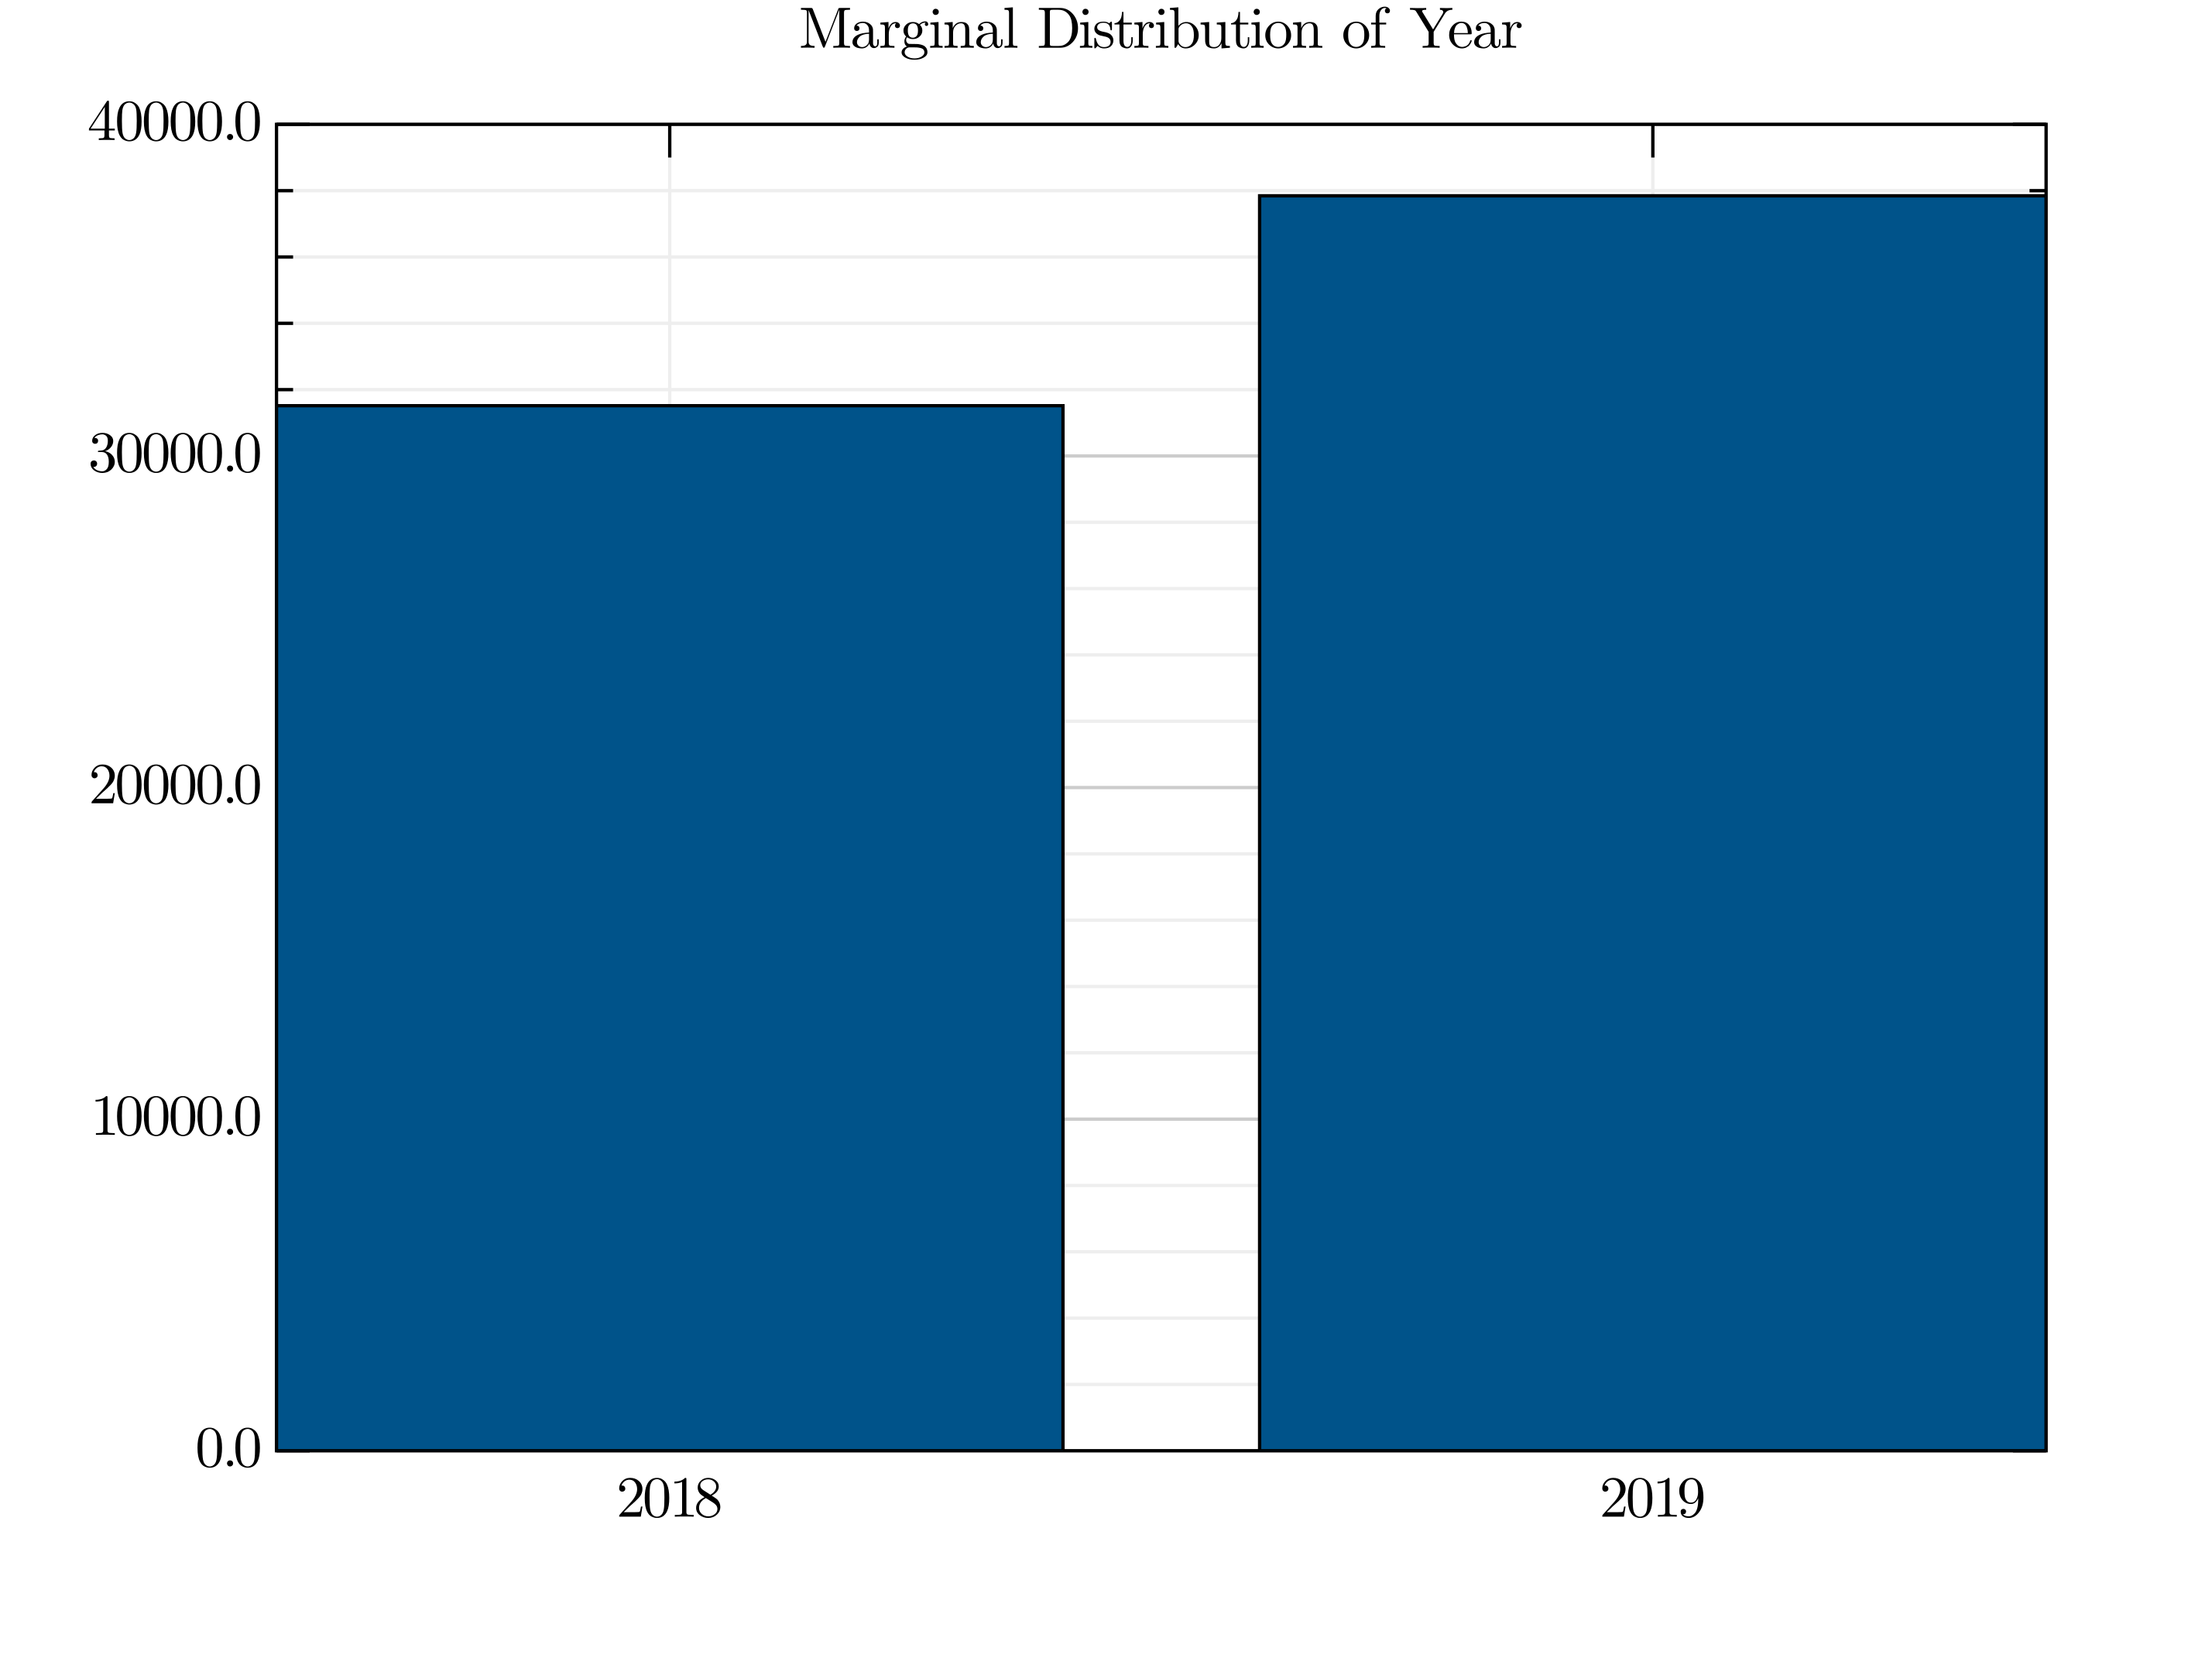
\includegraphics{visuals/marginals_YR.png}
\caption{Judge Origin Marginal}
\end{figure}
 \begin{figure}
\centering
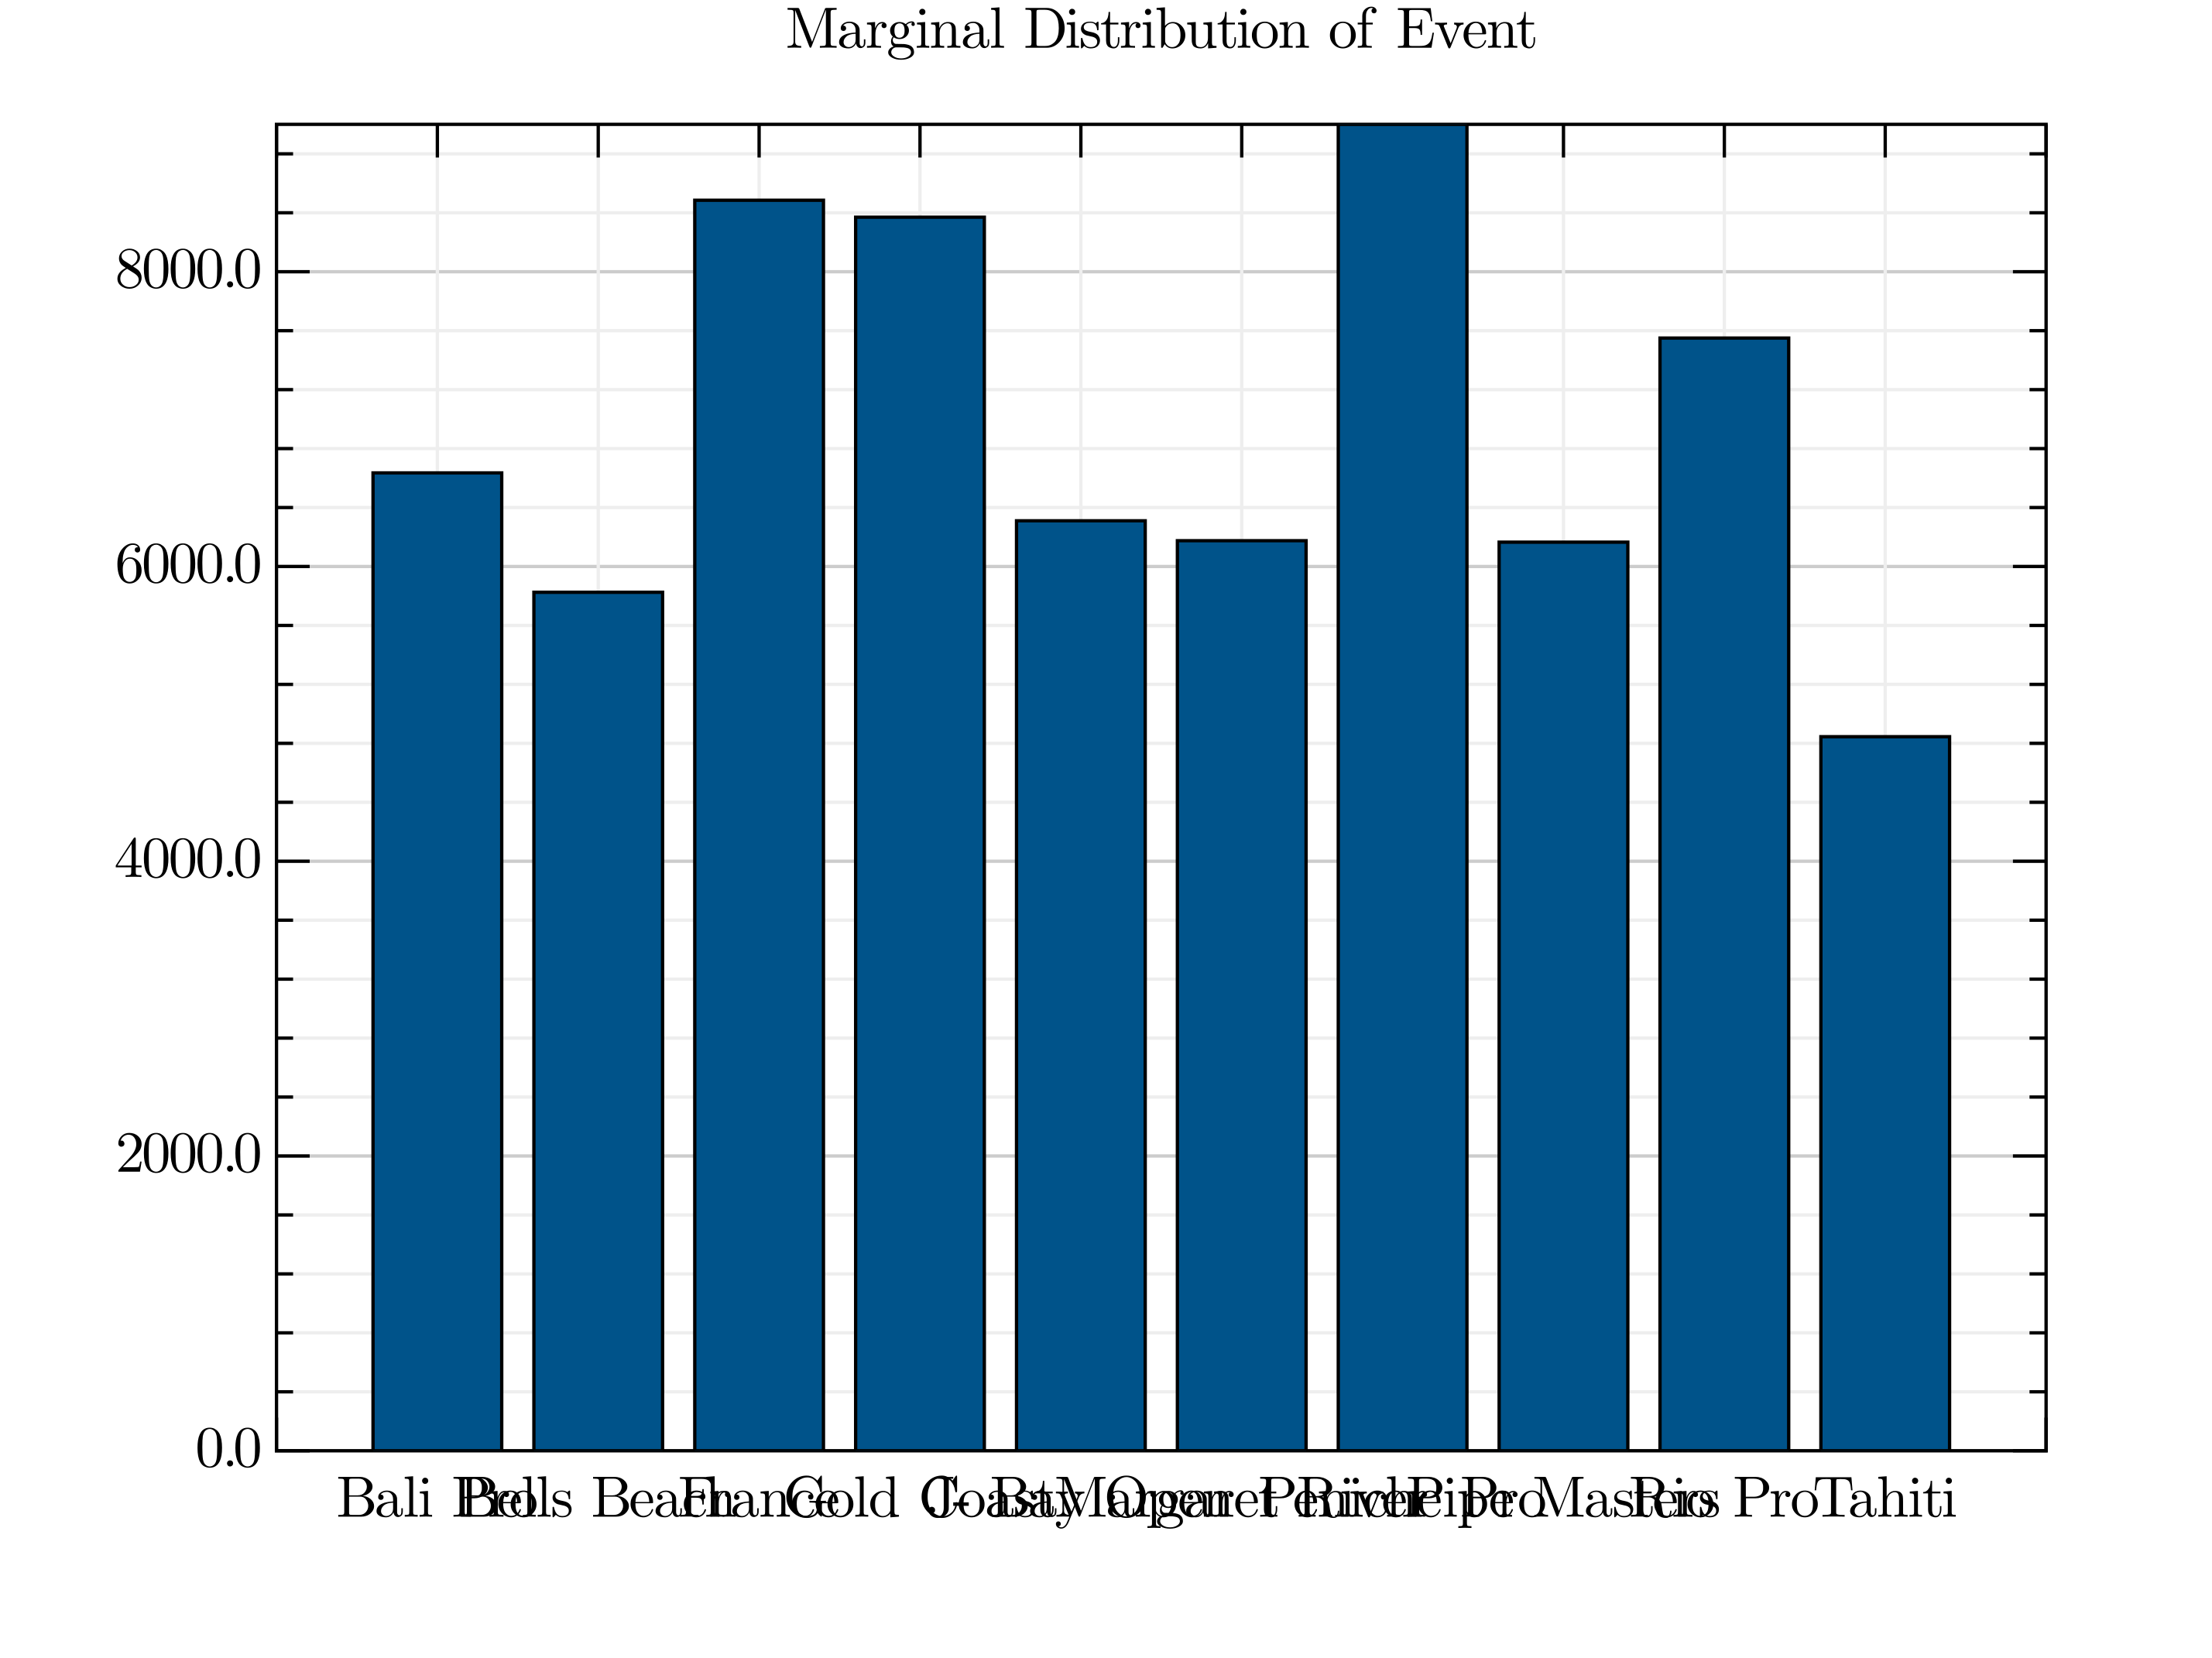
\includegraphics{visuals/marginals_EVT.png}
\caption{Judge Origin Marginal}
\end{figure}
 \begin{figure}
\centering
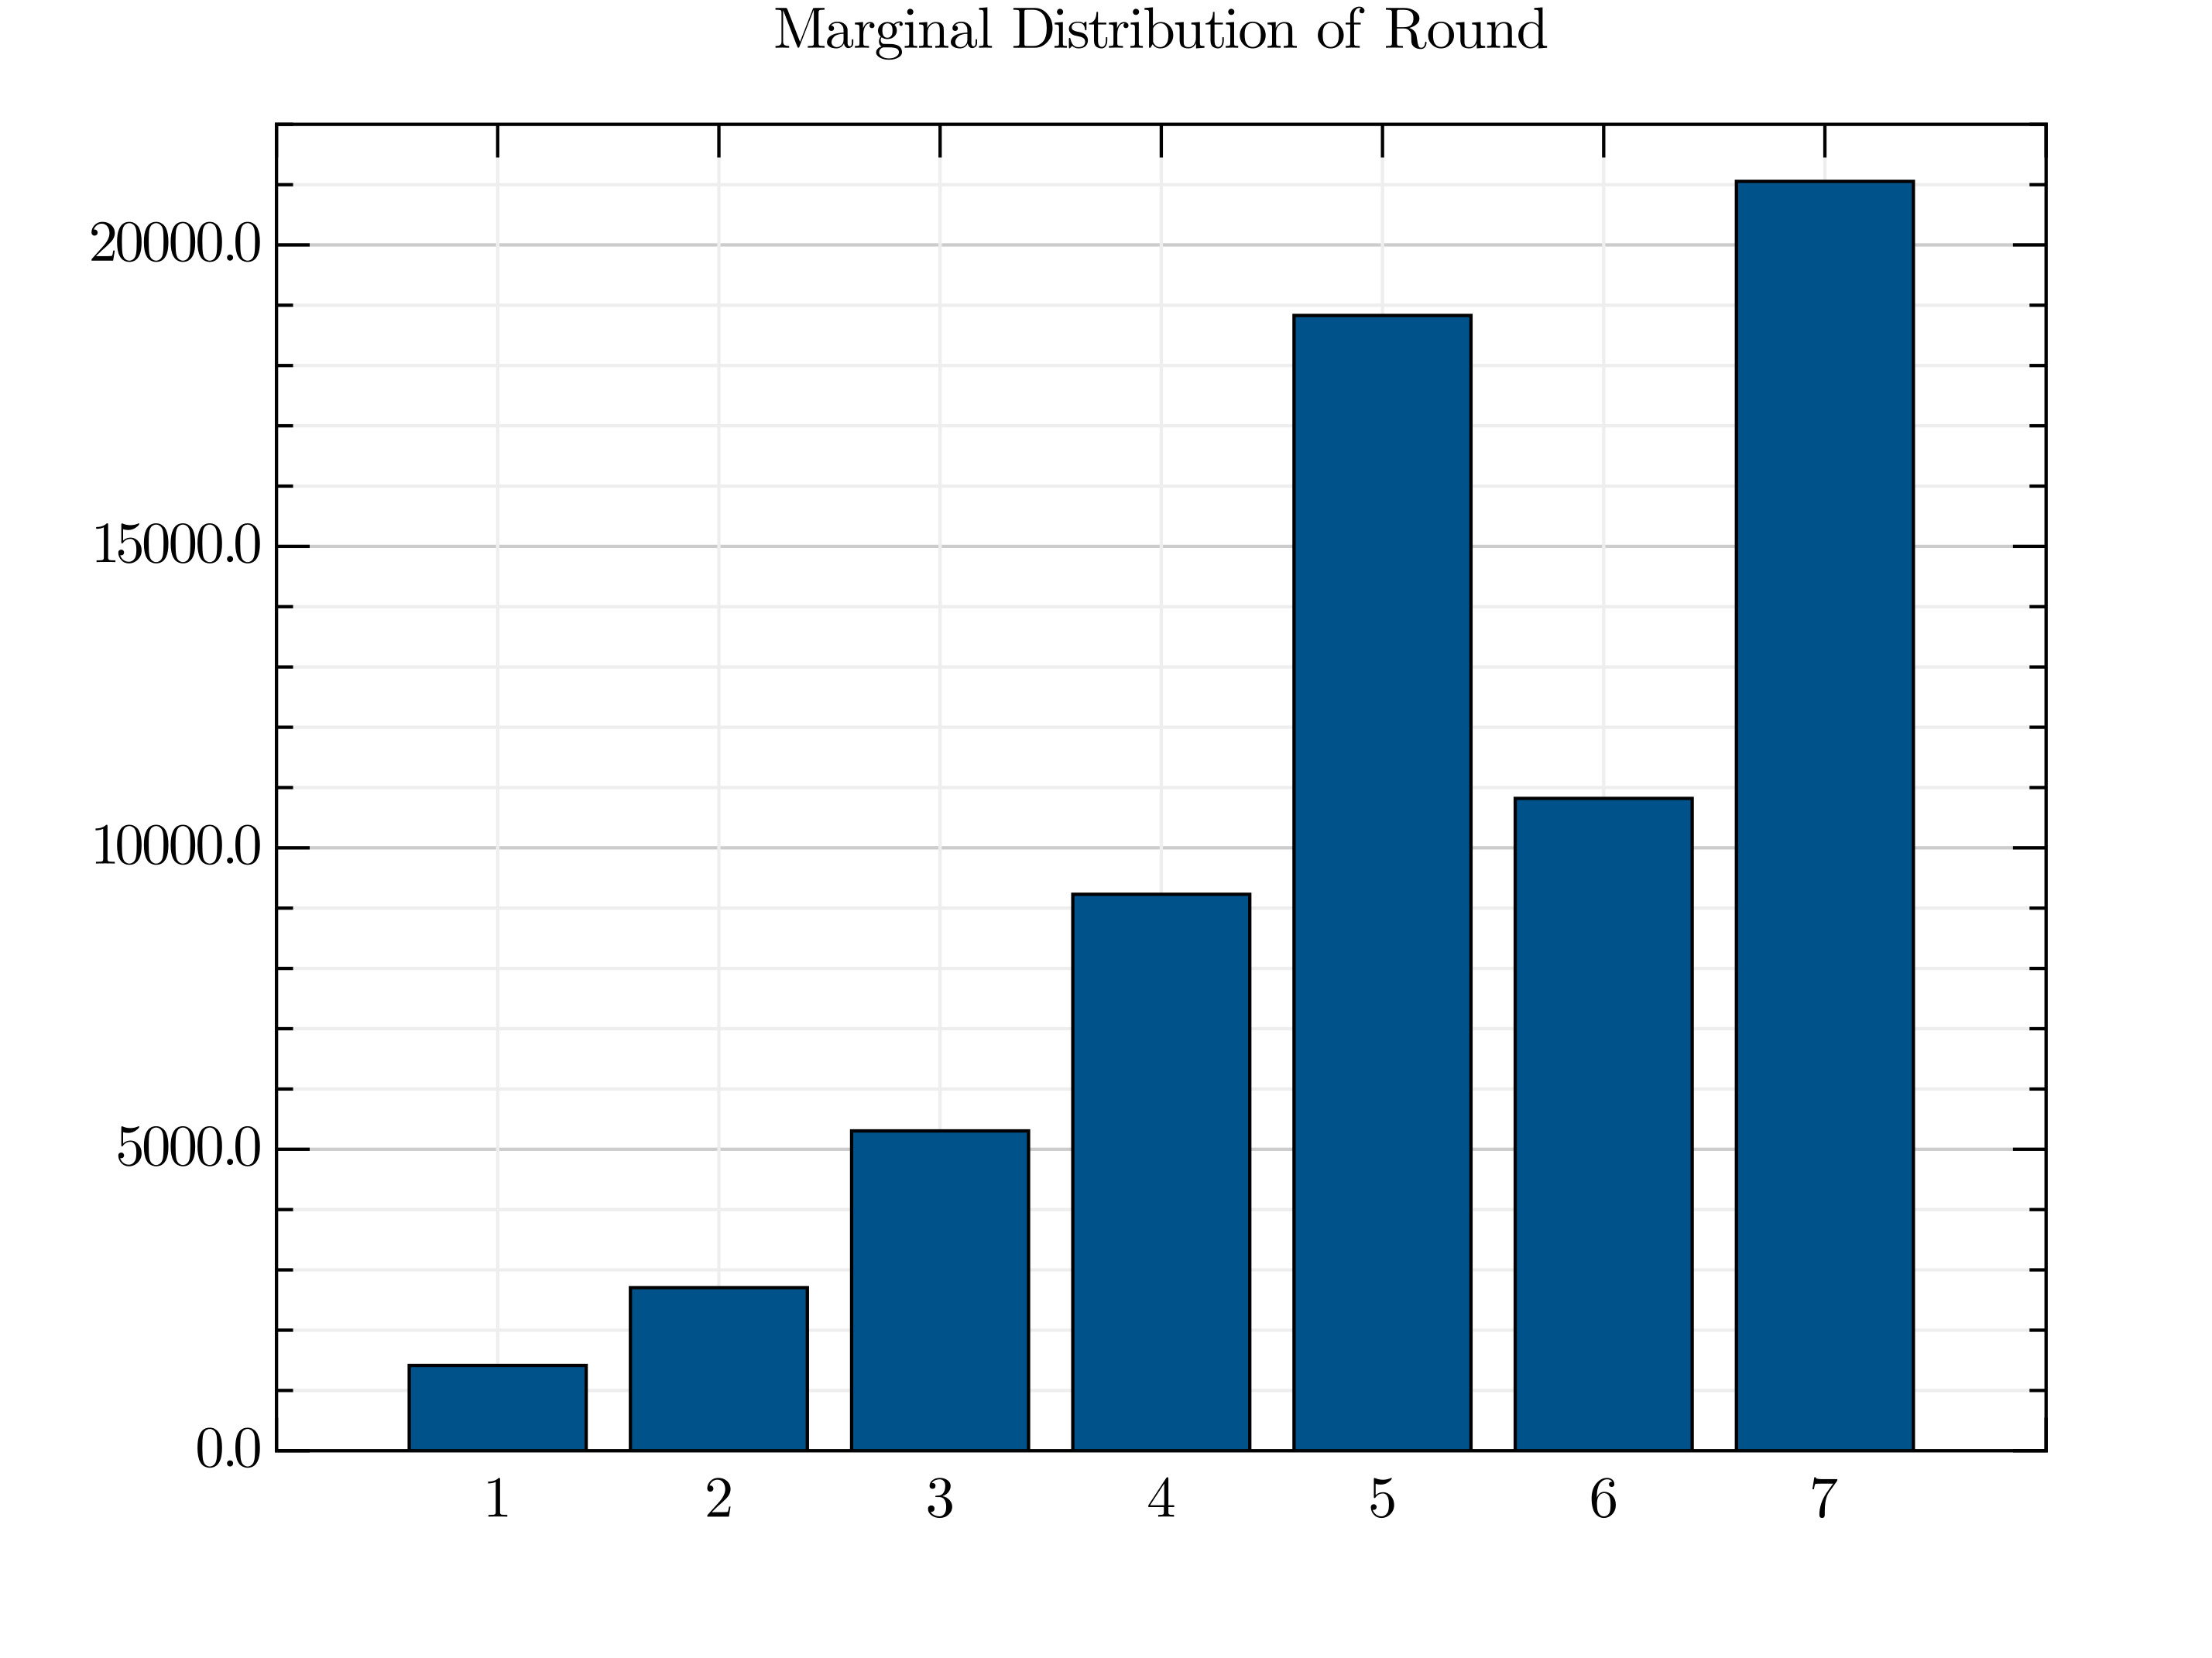
\includegraphics{visuals/marginals_RND.png}
\caption{Judge Origin Marginal}
\end{figure}
 \begin{figure}
\centering
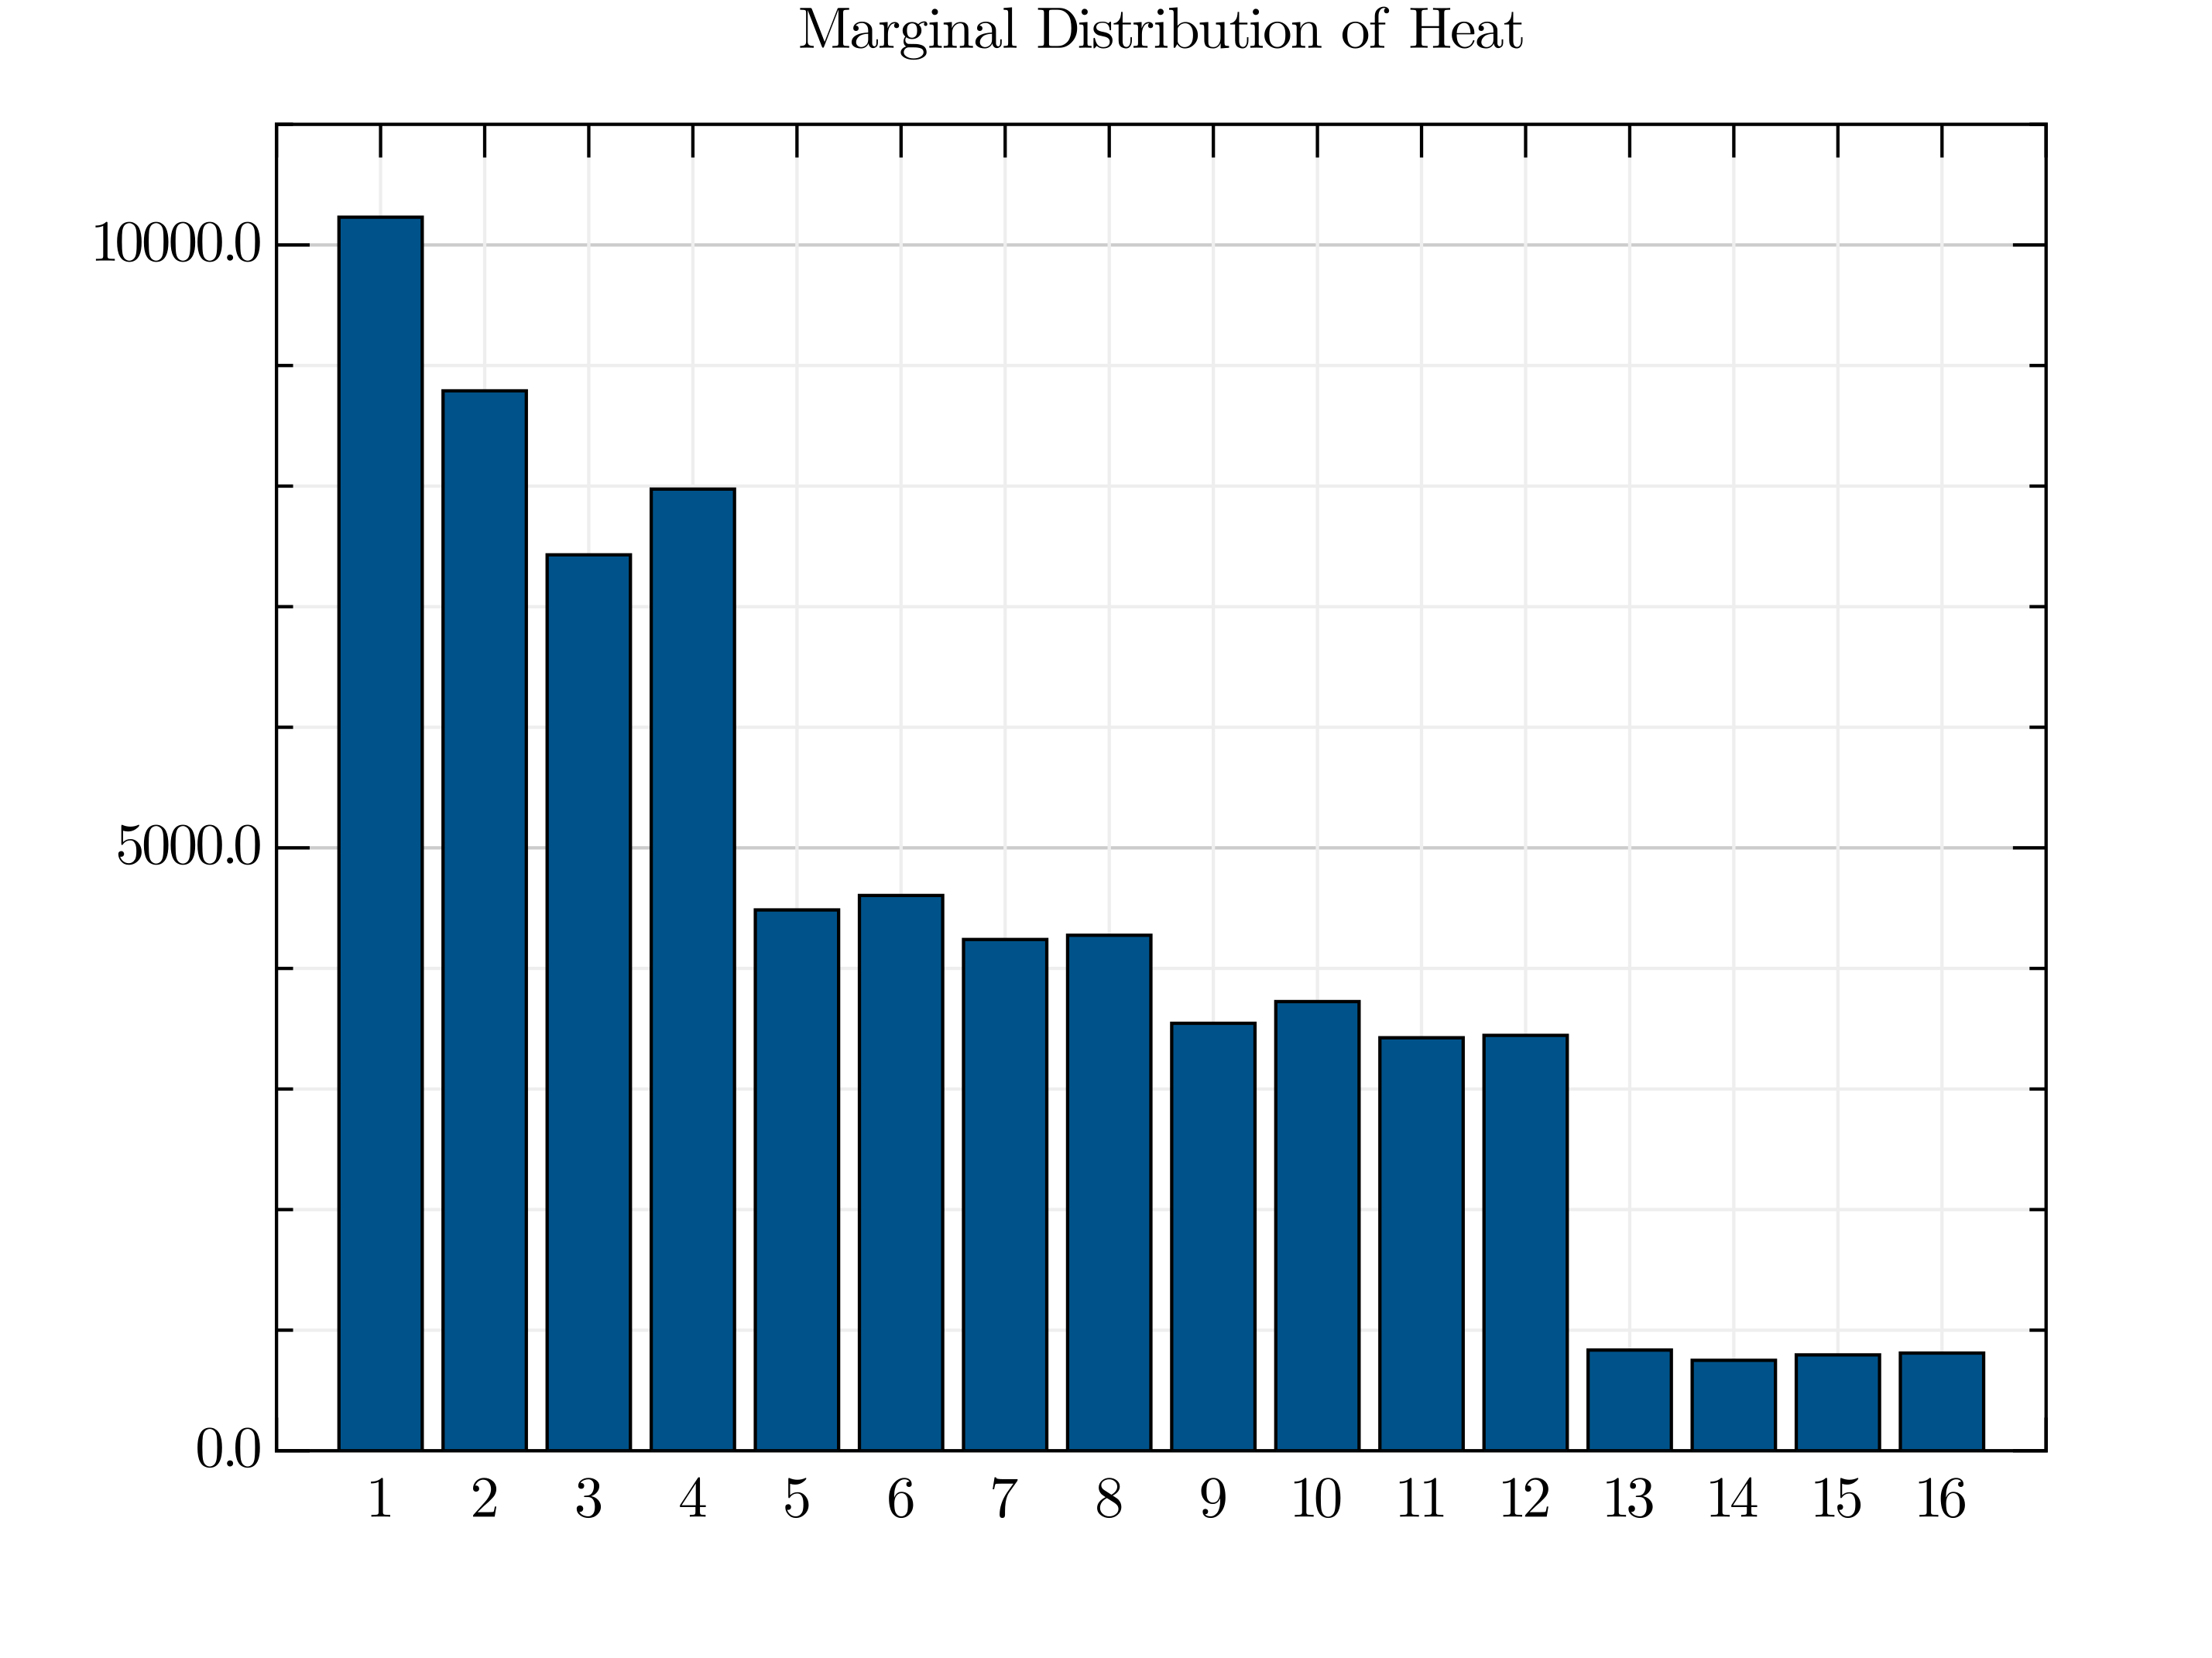
\includegraphics{visuals/marginals_HEAT.png}
\caption{Judge Origin Marginal}
\end{figure}
 \begin{figure}
\centering
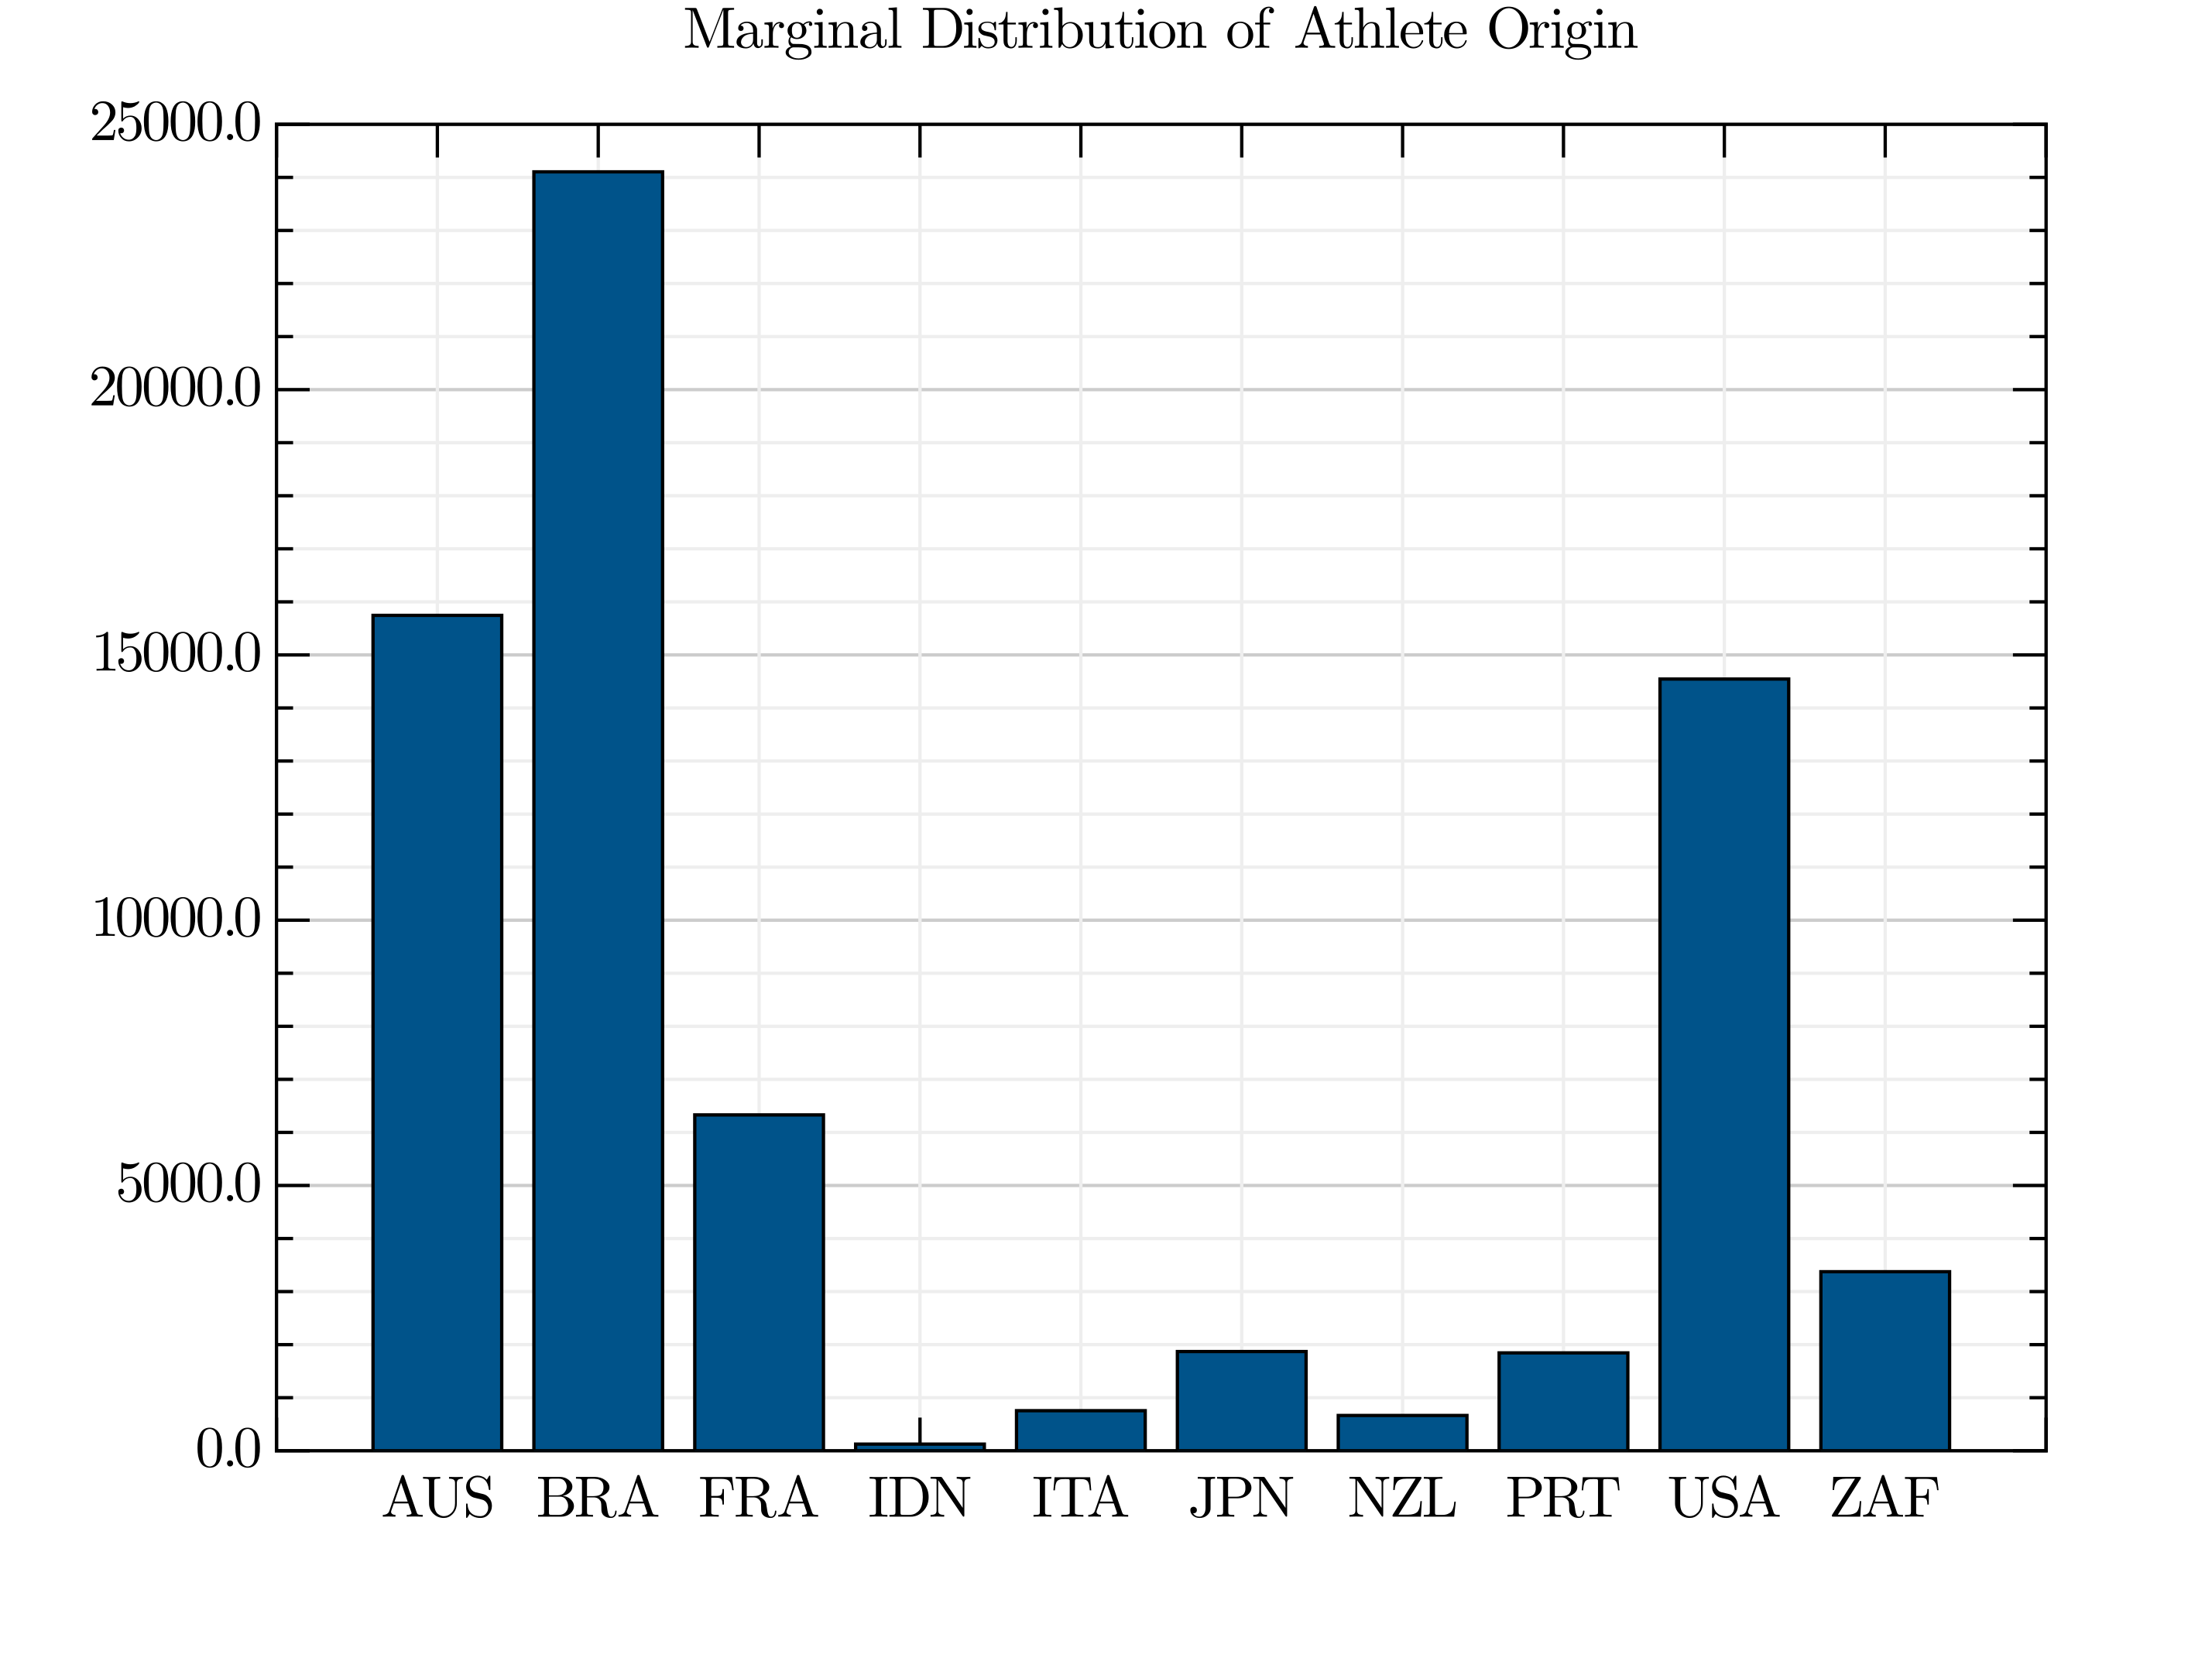
\includegraphics{visuals/marginals_ATH_orig.png}
\caption{Judge Origin Marginal}
\end{figure}
 \begin{figure}
\centering
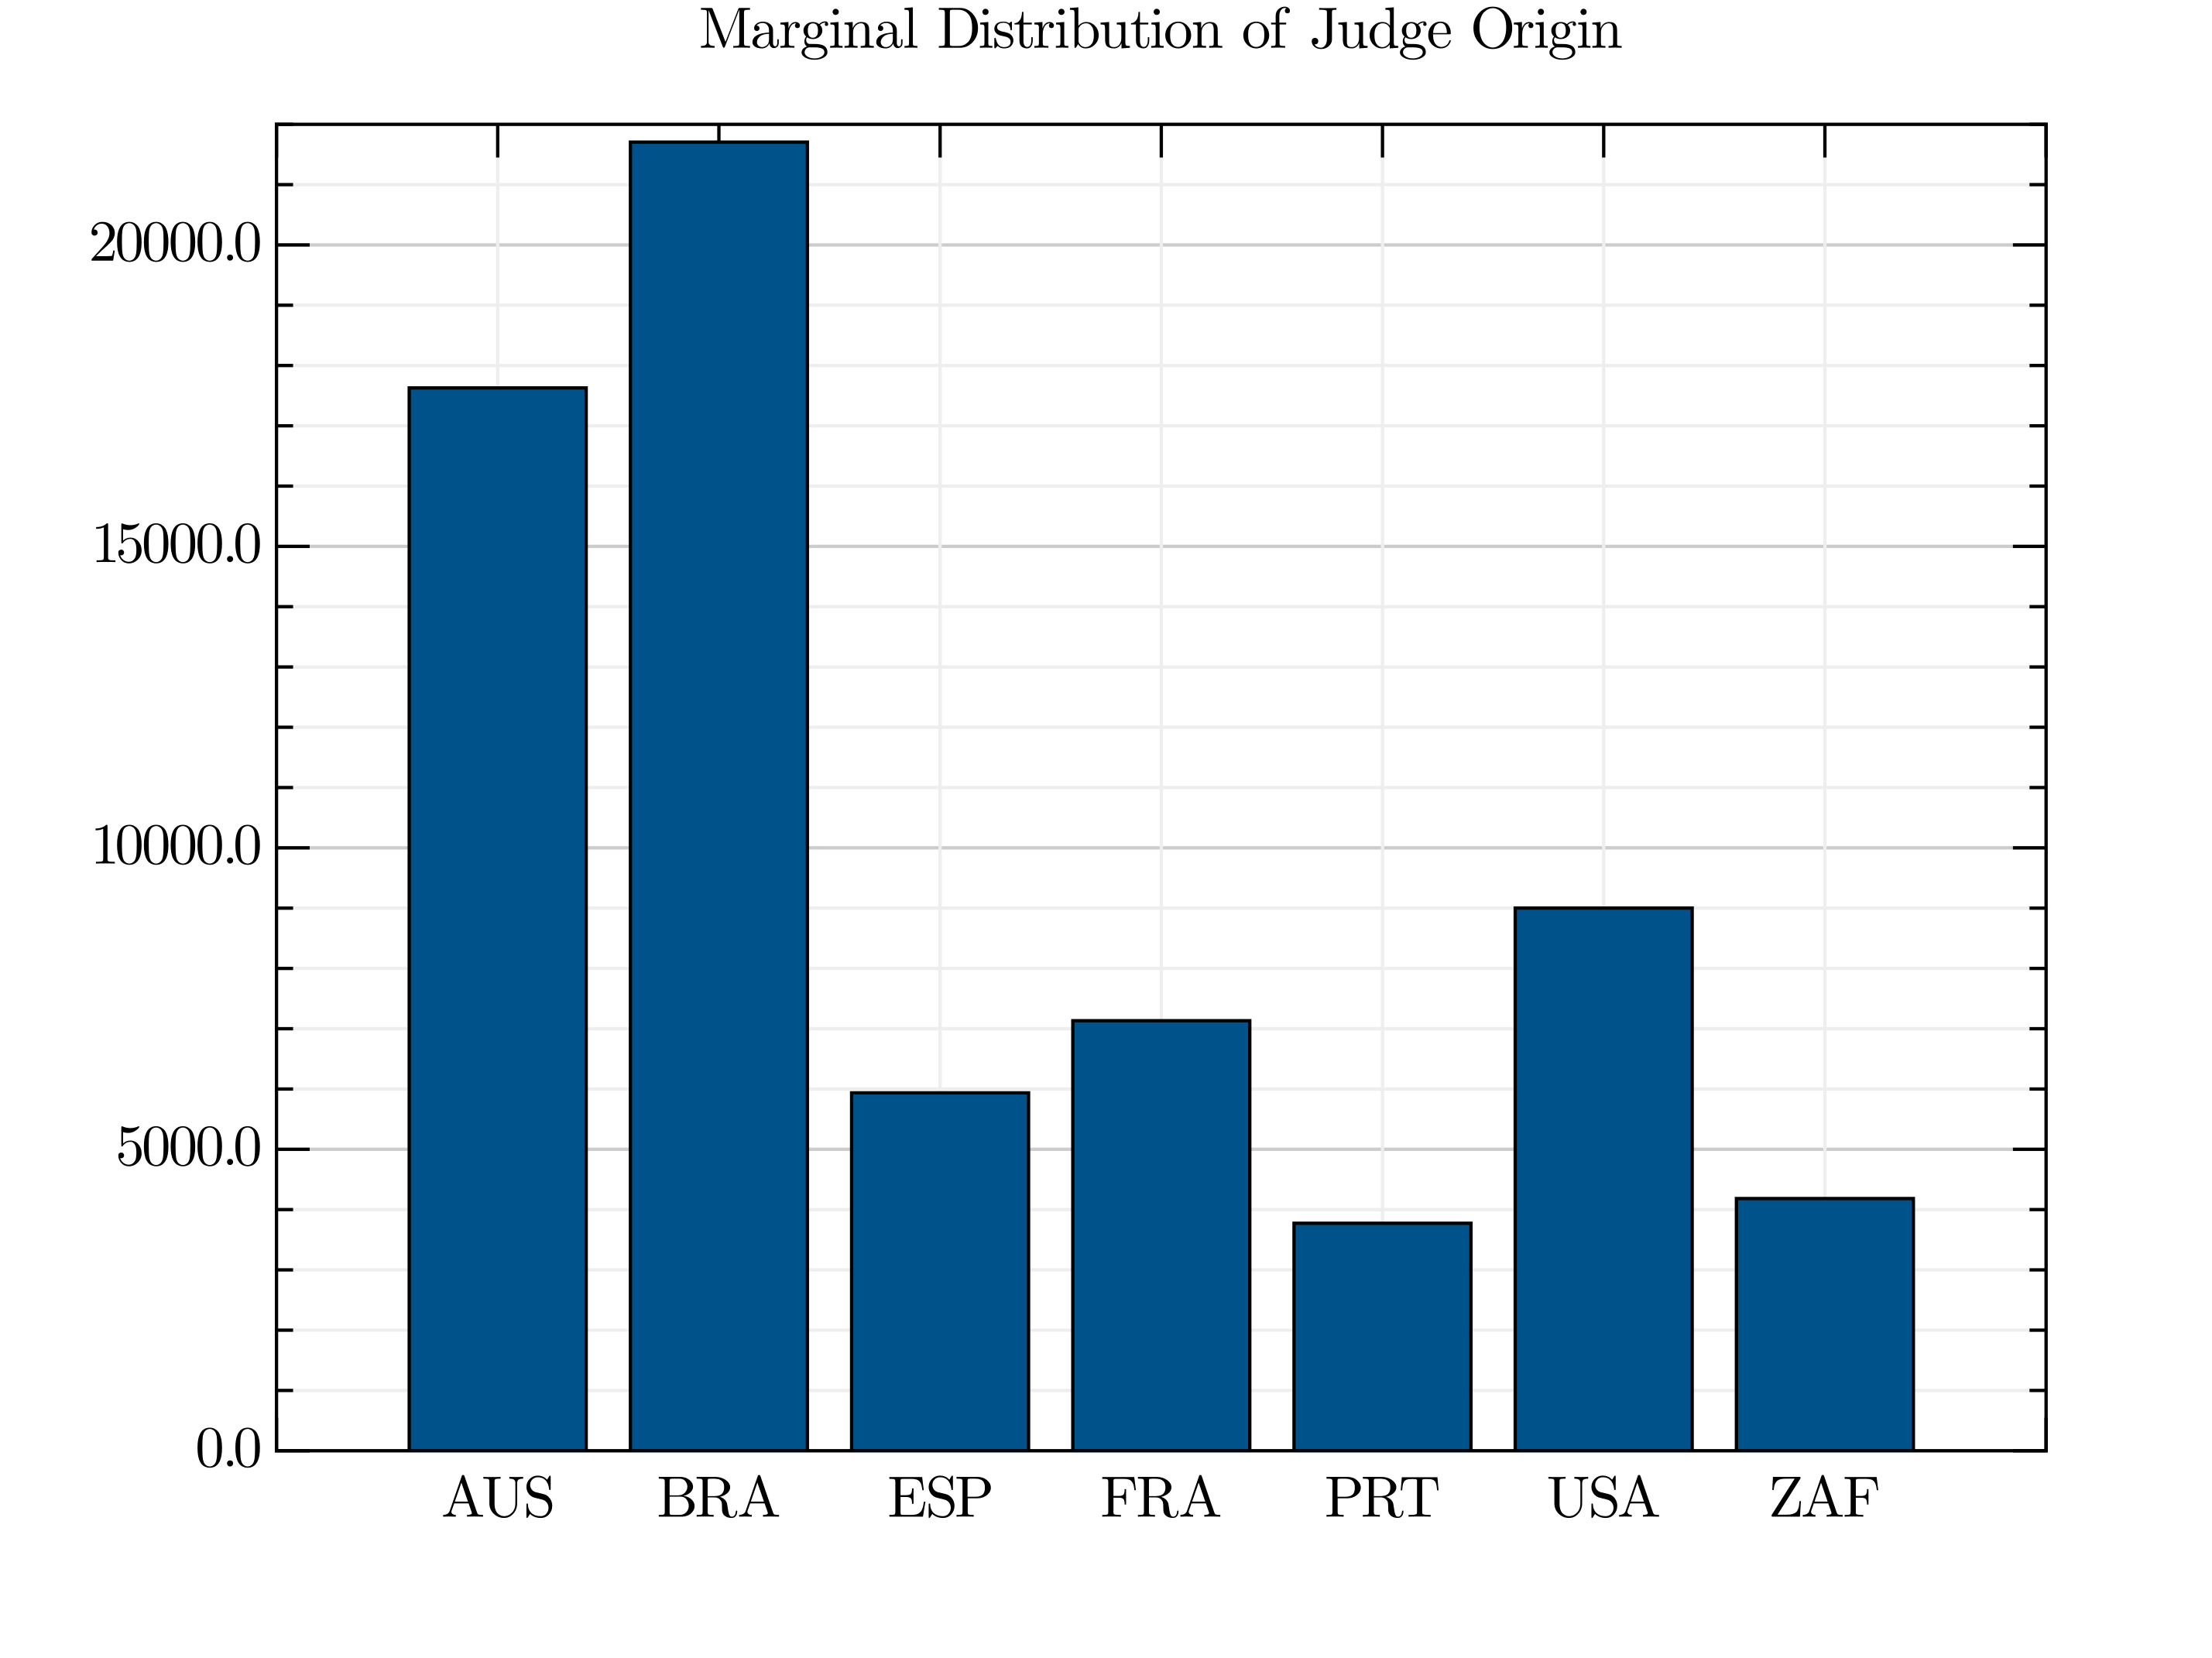
\includegraphics{visuals/marginals_JUD_orig.png}
\caption{Judge Origin Marginal}
\end{figure}
 \begin{figure}
\centering
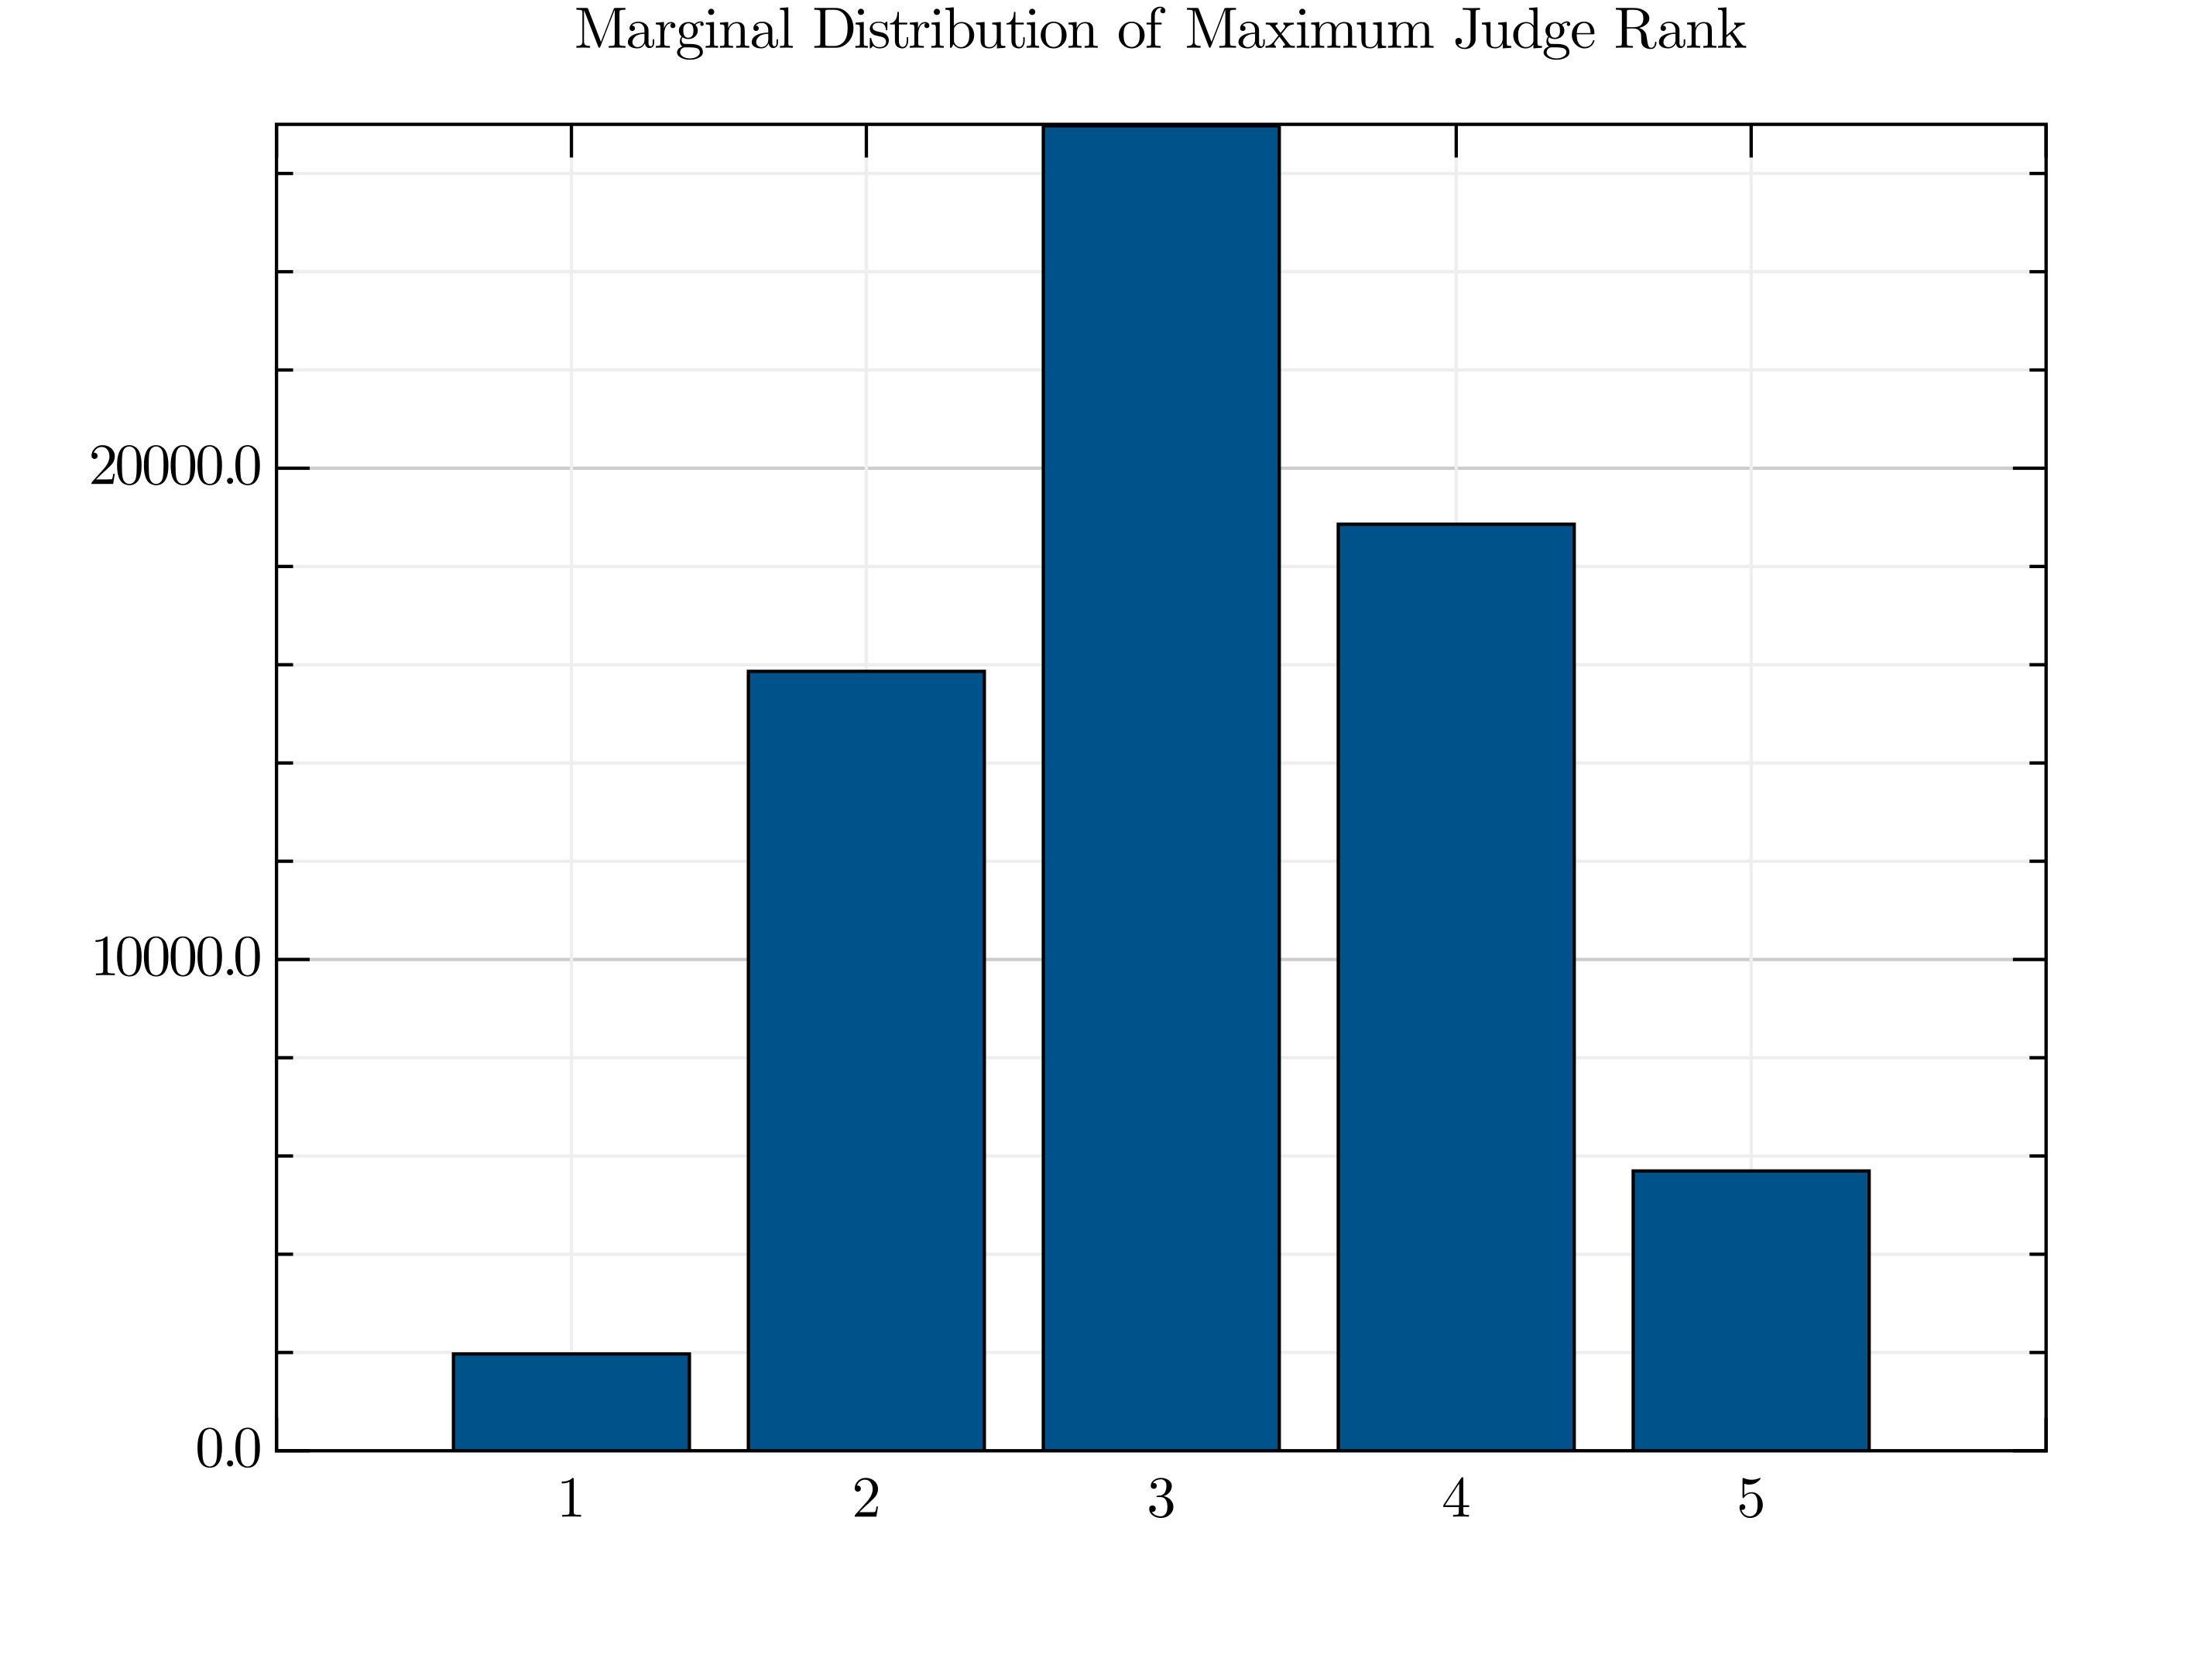
\includegraphics{visuals/marginals_MAX_RANK.png}
\caption{Judge Origin Marginal}
\end{figure}
 \begin{figure}
\centering
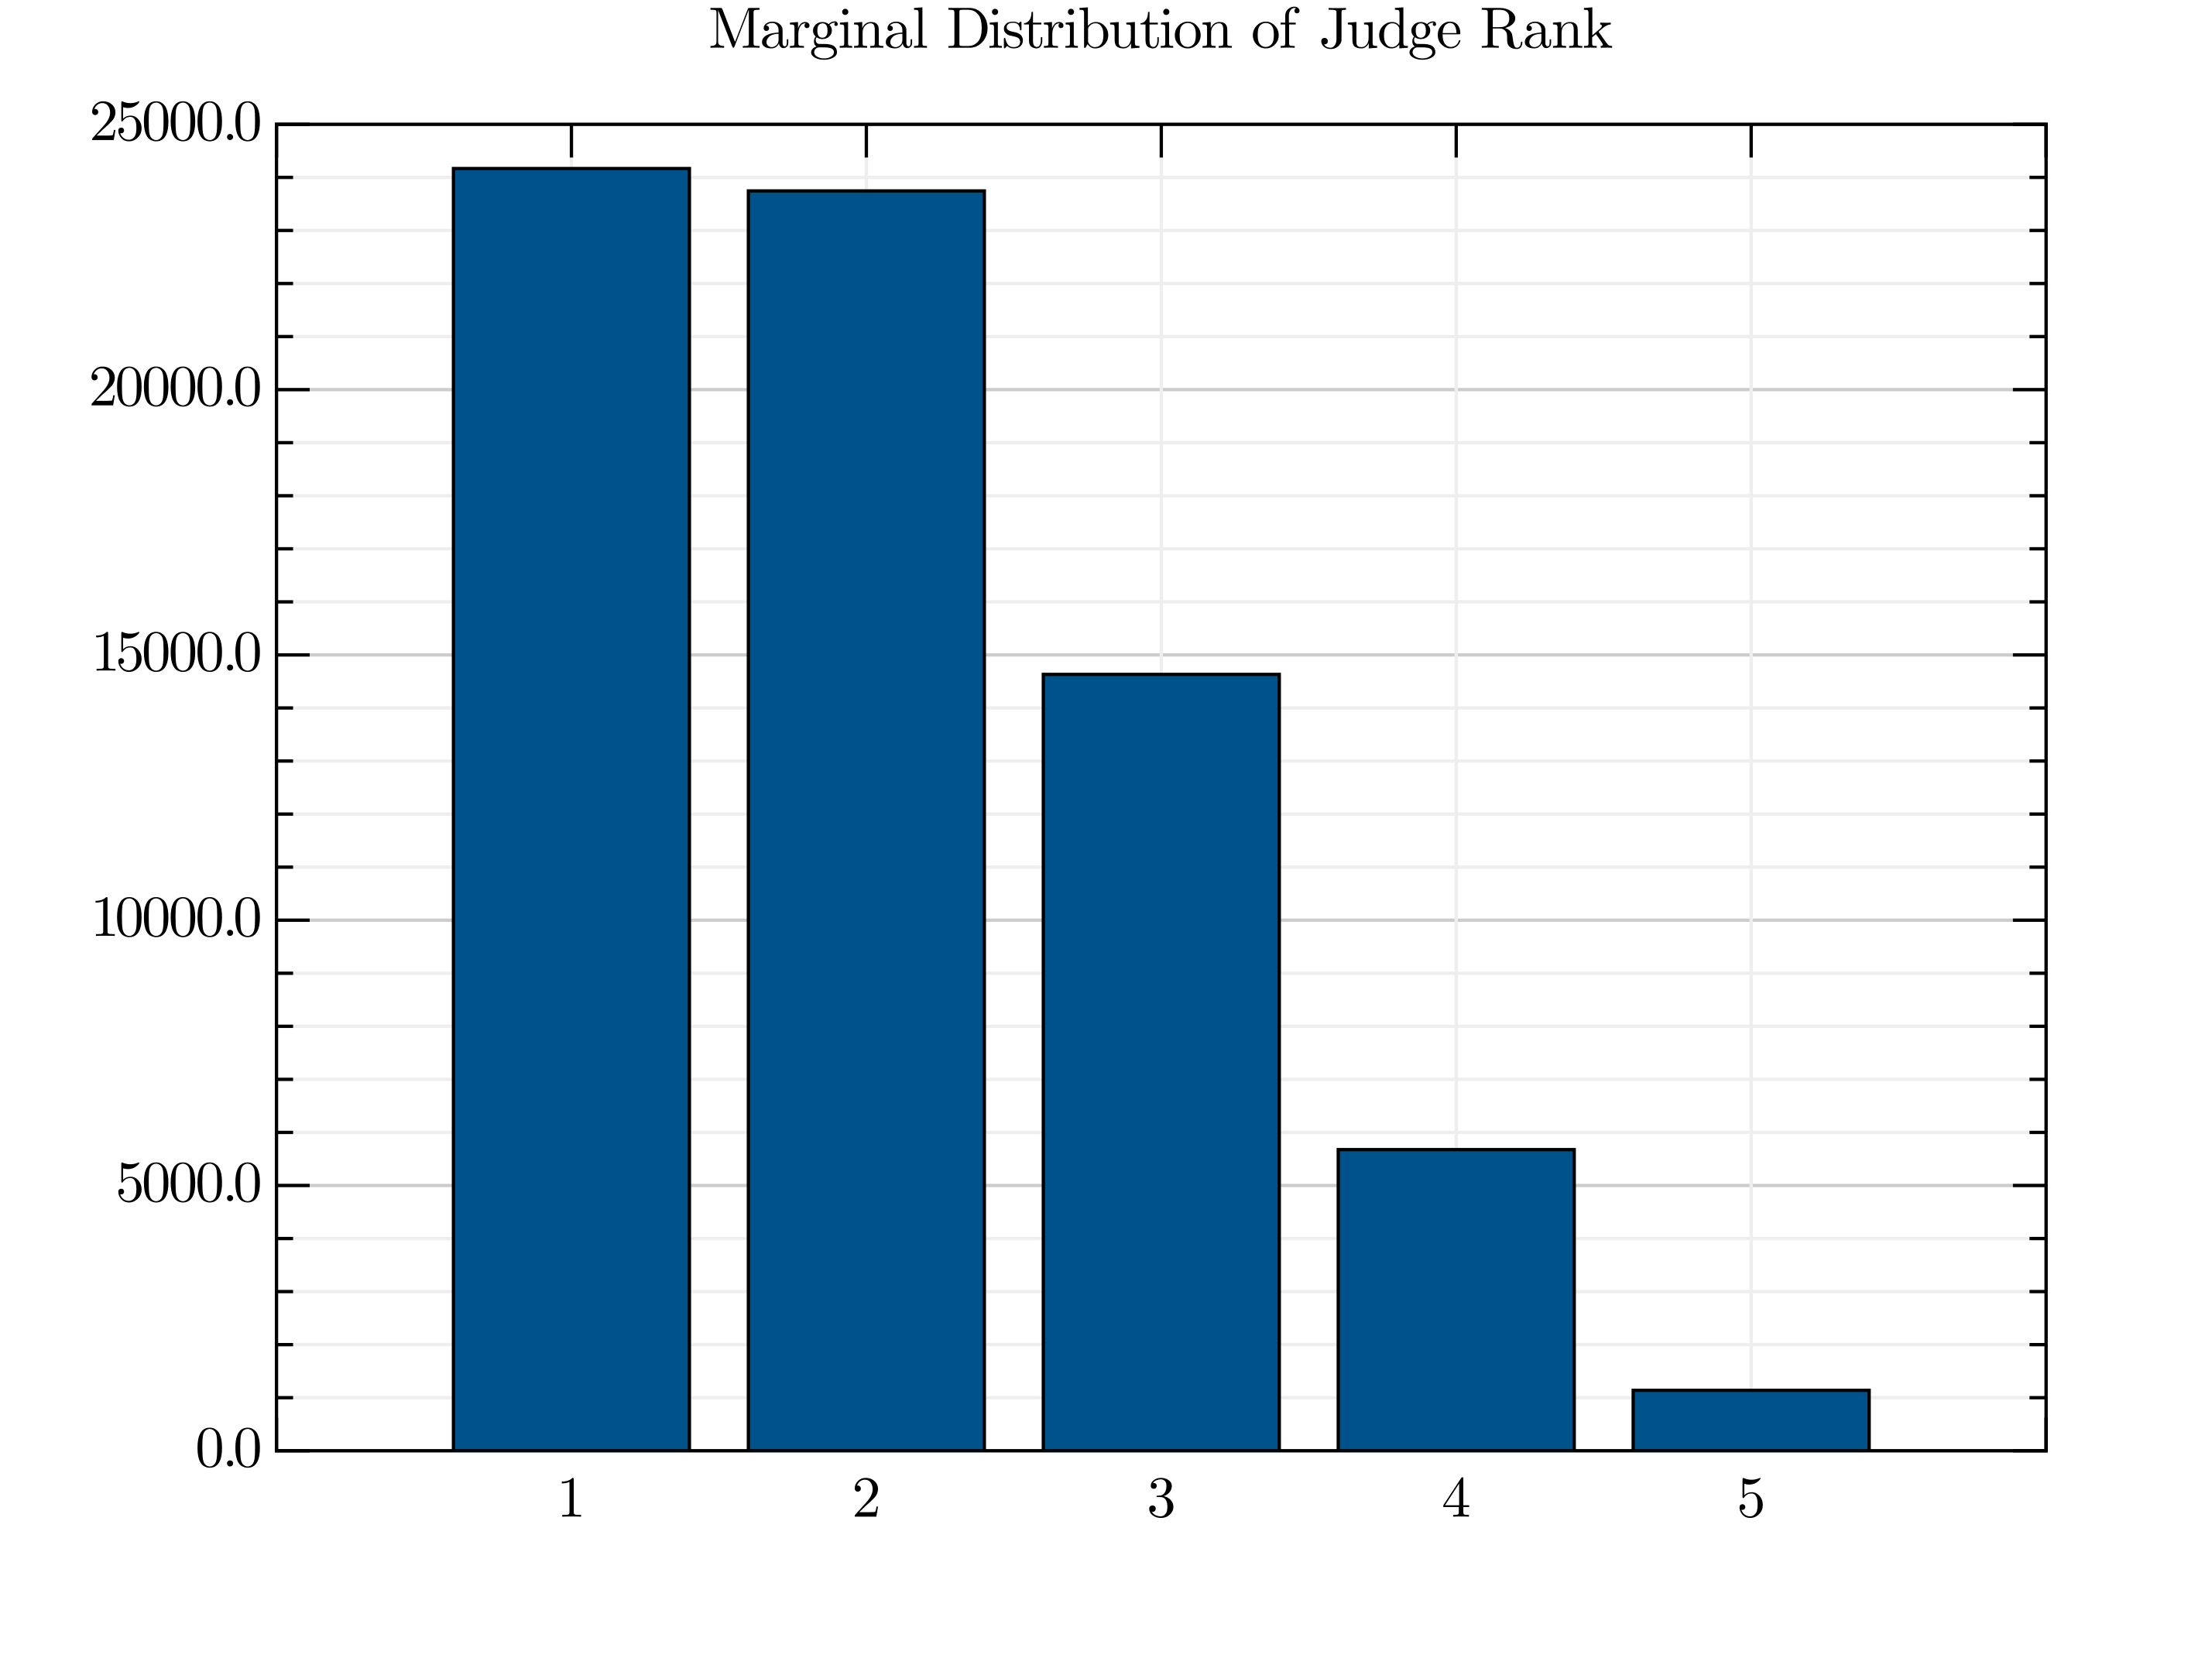
\includegraphics{visuals/marginals_RANK.png}
\caption{Judge Rank Marginal}
\end{figure}



\section{Definitions}
\begin{itemize}
\item \textbf{The Symmetric Group on a set, $X$} is $S_X := Isomorphisms(X,X)$. When |X|<\ensuremath{\infty},$S_X = \{ \ensuremath{\tau}:X\ensuremath{\rightarrow}X | Image(\ensuremath{\tau}) = X \}  = \{\ensuremath{\tau}:X\ensuremath{\rightarrow}X \ensuremath{\mid} \{\ensuremath{\tau}(x) \ensuremath{\mid} x\ensuremath{\in}X \} = X \}$


\item $S\ensuremath{\_k} := S_{\{ 1,\ensuremath{\ldots},k\} }.$


\item When G is a Group, and \ensuremath{\bbF} is a Field, the **Group Algebra of G over \ensuremath{\bbF} **, denoted \ensuremath{\bbF}[G], is the space of formal linear combinations of elements of G. Elements of \ensuremath{\bbF}[G] are of the form: $c\ensuremath{\_1}g\ensuremath{\_1} + \ensuremath{\ldots} + c\ensuremath{\_n}g\ensuremath{\_n} = \ensuremath{\sum}^n_{i=1} c\ensuremath{\_i}g\ensuremath{\_i}$, where $c\ensuremath{\_i}\ensuremath{\in}\ensuremath{\bbF}, g\ensuremath{\_i}\ensuremath{\in}G$. Note that i=\ensuremath{\not}j \ensuremath{\Longrightarrow} g\ensuremath{\_i} =\ensuremath{\not} g\ensuremath{\_j} because G is a set of elements, so no element occurs with multiplicity. For example, c\ensuremath{\_1}g + c\ensuremath{\_2}g \ensuremath{\in}\ensuremath{\not} \ensuremath{\bbF}[G] whereas (c\ensuremath{\_1}+c\ensuremath{\_2})g \ensuremath{\in} \ensuremath{\bbF}[G].


\item \ensuremath{\bbF}[S\ensuremath{\_k}] is comprised on formal linear combinations of elements of S\ensuremath{\_k}. This may be understood as two different ways:

\begin{itemize}
\item There exists a function a:S\ensuremath{\_k}\ensuremath{\rightarrow}\ensuremath{\bbF} and $A:=\ensuremath{\sum}_{\ensuremath{\tau}\ensuremath{\in}S\ensuremath{\_k}} a(\ensuremath{\tau})\ensuremath{\tau}$ \ensuremath{\in} \ensuremath{\bbF}[S\ensuremath{\_k}].


\item Or: $A = [ \ensuremath{\pi}\ensuremath{\_1} \ensuremath{\ldots}  \ensuremath{\pi}_{k!} ] \begin{bmatrix}a_{\pi_1} \\ \vdots  \\ a_{\ensuremath{\pi}_{k!}} \end{bmatrix} = \sum_{\tau \in S\ensuremath{\_k} } a_\ensuremath{\tau} \ensuremath{\tau} \ensuremath{\in} \ensuremath{\bbF}[S\ensuremath{\_k}]$,where \ensuremath{\tau} \ensuremath{\in} S\ensuremath{\_k} and a\_\ensuremath{\tau} \ensuremath{\in}\ensuremath{\bbF}.

\end{itemize}

\item **Addition in \ensuremath{\bbF}[S\ensuremath{\_k}] ** is defined by $A+B = (\ensuremath{\sum}_{\ensuremath{\tau}} a_\ensuremath{\tau} \ensuremath{\tau}) + (\ensuremath{\sum}_\ensuremath{\tau} b_\ensuremath{\tau} \ensuremath{\tau}) := \ensuremath{\sum}_\ensuremath{\tau} (a_\ensuremath{\tau} + b_\ensuremath{\tau}) \ensuremath{\tau}$


\item \textbf{Scalar Multiplication in $\ensuremath{\bbF}[S\ensuremath{\_k}]$} is $c(A) = c(\ensuremath{\sum}_{\ensuremath{\tau}} a_\ensuremath{\tau} \ensuremath{\tau})  = \ensuremath{\sum}_{\ensuremath{\tau}} ca_\ensuremath{\tau} \ensuremath{\tau}$.


\item Multiplication in \ensuremath{\bbF}[S\ensuremath{\_k}] is \emph{defined} by: $A*B =(\ensuremath{\sum}_{\ensuremath{\tau}} a_\ensuremath{\tau} \ensuremath{\tau})* (\ensuremath{\sum}_\ensuremath{\pi} b_\ensuremath{\pi} \ensuremath{\pi}) :=\ensuremath{\sum}_{\ensuremath{\gamma} \ensuremath{\in} S\ensuremath{\_k}}(\ensuremath{\sum}_{\ensuremath{\tau},\ensuremath{\pi} | \ensuremath{\tau}\ensuremath{\pi}=\ensuremath{\gamma}} a_\ensuremath{\tau} b_\ensuremath{\pi}) \ensuremath{\gamma} = \ensuremath{\sum}_{\ensuremath{\gamma} \ensuremath{\in} S\ensuremath{\_k}}(\ensuremath{\sum}_{\ensuremath{\tau} \ensuremath{\in} S\ensuremath{\_k}} a_\ensuremath{\tau} b_{\ensuremath{\tau}^{-1}\ensuremath{\gamma}})\ensuremath{\gamma}$.

\end{itemize}

We should not over complicate $*$. The \emph{definition} of $*$ may look odd, but it exactly the same as our basic understanding of multiplication: $(\sum_{  \tau} a_\tau\tau) *(\sum_{\pi }   b_\pi \pi) = \sum_{  \tau} (a_\tau\tau) *(\sum_{\pi }   b_\pi \pi) = \sum_{  \tau} \sum_{\pi }  (a_\tau\tau) * (b_\pi \pi) = \sum_{  \tau}\sum_{\pi } a_\tau b_\pi \tau \pi =\sum_{\gamma \in S_d}(\sum_{  \tau,\pi | \tau\pi = \gamma  } a_\tau b_\pi) \gamma =(\sum_{\tau} a_\tau \tau)* (\sum_\pi b_\pi \pi)$ Even though $(\ensuremath{\sum}_{\ensuremath{\tau}} a_\ensuremath{\tau} \ensuremath{\tau}) *(\ensuremath{\sum}_{\ensuremath{\pi}} b_\ensuremath{\pi} \ensuremath{\pi})$ is equal to the intuitive form, $\ensuremath{\sum}_{\ensuremath{\tau}}\sum_{\ensuremath{\pi}} a_\ensuremath{\tau} b_\ensuremath{\pi} \ensuremath{\tau}\ensuremath{\pi}$, the latter is not an element of the the group algebra because elements are repeated in the sum, hence our chosen definition. Also, $*$ merely extends multiplication in the Field,$\cdot: \mathbb{F} \times \mathbb{F} \rightarrow \mathbb{F}$, and the operation in the group, $\ensuremath{\circ}$, by $a_\ensuremath{\tau} \ensuremath{\tau} * b_\ensuremath{\pi} \ensuremath{\pi} = a_\ensuremath{\tau}\ensuremath{\cdot}b_\ensuremath{\pi} \ensuremath{\tau}\ensuremath{\circ}\ensuremath{\pi} = a_\ensuremath{\tau} b_\ensuremath{\pi} \ensuremath{\tau}\ensuremath{\pi}$, where the last equality is simply notation-reduction.

A measure on S\ensuremath{\_k}, is an element of the group algebra $\ensuremath{\bbC}[S\ensuremath{\_k}]$. A measure on S\ensuremath{\_k}, $F = \ensuremath{\sum}_{\ensuremath{\tau} \ensuremath{\in} S\ensuremath{\_k}} f_\ensuremath{\tau} \ensuremath{\tau}$, is a probability measure on S\ensuremath{\_k} if and only if $\ensuremath{\forall} \ensuremath{\tau} \ensuremath{\in} S\ensuremath{\_k} f_\ensuremath{\tau} \ensuremath{\geq} 0$ and $\ensuremath{\sum}_{\ensuremath{\tau} \ensuremath{\in} S\ensuremath{\_k}} f_\ensuremath{\tau} = 1$.

A linear representation of a group G, is a group homomorphism, $\ensuremath{\rho} : (G,\ensuremath{\circ}) \ensuremath{\rightarrow} (GL(V),\ensuremath{\cdot})$. A group homomorphism satisfies:

\begin{itemize}
\item \ensuremath{\forall} x,y \ensuremath{\in} G \ensuremath{\rho}(x\ensuremath{\circ}y) = \ensuremath{\rho}(x)\ensuremath{\cdot}\ensuremath{\rho}(y) where \ensuremath{\cdot} is multiplication in GL(V).


\item \ensuremath{\rho}(e) = I, where e is the identity element in G and I is the identity element in GL(V).


\item $\ensuremath{\forall} x \ensuremath{\in} G, \ensuremath{\rho}(x^{-1}) = \ensuremath{\rho}(x)^*$, where $^*$ denotes involution in GL(V).

\end{itemize}

The representation of a measure F, is:$F\ensuremath{\hat} := \ensuremath{\sum}_{\ensuremath{\tau} \ensuremath{\in} S\ensuremath{\_k}} F(\ensuremath{\tau})\ensuremath{\rho}(\ensuremath{\tau})$. Note: This is sometimes called the Fourier transform at a representation, I avoid that lingo. 

**Convolution of two functions on S\ensuremath{\_k} ** is a binary operation $A * B := \ensuremath{\sum}_{\ensuremath{\tau} \ensuremath{\in} S\ensuremath{\_k}} a(\ensuremath{\tau}) b(\ensuremath{\tau}^{-1}g)$.

Note: $\widehat{A*B} = \ensuremath{\sum}_{\ensuremath{\gamma}} (A*B)(\ensuremath{\gamma})\ensuremath{\rho}(\ensuremath{\gamma})  = \ensuremath{\sum}_{\ensuremath{\gamma}} \ensuremath{\sum}_{\ensuremath{\tau}} a(\ensuremath{\gamma} \ensuremath{\tau}^{-1})b(\ensuremath{\tau})\ensuremath{\rho}(\ensuremath{\gamma} ) = \ensuremath{\sum}_{\ensuremath{\tau}} \ensuremath{\sum}_{\ensuremath{\gamma}\ensuremath{\tau}} a(\ensuremath{\gamma} \ensuremath{\tau} \ensuremath{\tau}^{-1})b(\ensuremath{\tau})\ensuremath{\rho}(\ensuremath{\gamma}\ensuremath{\tau}) = \ensuremath{\sum}_{\ensuremath{\tau}} \ensuremath{\sum}_{\ensuremath{\gamma}\ensuremath{\tau}} a(\ensuremath{\gamma})b(\ensuremath{\tau})\ensuremath{\rho}(\ensuremath{\gamma})\ensuremath{\rho}(\ensuremath{\tau}) = \ensuremath{\sum}_{\ensuremath{\tau}} b(\ensuremath{\tau})\ensuremath{\rho}(\ensuremath{\tau}) \ensuremath{\sum}_{\ensuremath{\gamma}\ensuremath{\tau}} a(\ensuremath{\gamma})\ensuremath{\rho}(\ensuremath{\gamma})  = \ensuremath{\sum}_{\ensuremath{\tau}} b(\ensuremath{\tau})\ensuremath{\rho}(\ensuremath{\tau}) A\ensuremath{\hat} = A\ensuremath{\hat} \ensuremath{\sum}_{\ensuremath{\tau}} b(\ensuremath{\tau})\ensuremath{\rho}(\ensuremath{\tau}) = A\ensuremath{\hat} \ensuremath{\cdot} B\ensuremath{\hat}$

We take \ensuremath{\rho}\ensuremath{\_k} the permutation representation acting on the vector space V := \ensuremath{\bbR}\ensuremath{\^k} with basis indexed by \{1,\ensuremath{\ldots},k\}. So a typical element of V is of the form: 

$\begin{pmatrix} a^1 \\ a^2 \\ \ensuremath{\vdots} \\ a^k \end{pmatrix} = \begin{pmatrix} a^1 \\ 0 \\ \ensuremath{\vdots} \\ 0 \end{pmatrix} + \begin{pmatrix} 0 \\ a^2 \\ \ensuremath{\vdots} \\ 0 \end{pmatrix} + \ensuremath{\ldots} + \begin{pmatrix} 0 \\  \ensuremath{\vdots} \\ 0\\ a^k \end{pmatrix}  = a^1\begin{pmatrix} 1 \\ 0 \\ \ensuremath{\vdots} \\ 0 \end{pmatrix} + a^2\begin{pmatrix} 0 \\ 1 \\ \ensuremath{\vdots} \\ 0 \end{pmatrix} + \ensuremath{\ldots} + a^k\begin{pmatrix} 0 \\  \ensuremath{\vdots} \\ 0\\ 1\end{pmatrix}  = a^1 e\ensuremath{\_1} + a^2 e\ensuremath{\_2} + \ensuremath{\ldots} a^k e\ensuremath{\_k}$

This could be rewritten as $\ensuremath{\sum}_{i \ensuremath{\in} \{1,\ensuremath{\ldots},n\} } a^i e\ensuremath{\_i}$. But remember, we are interested in functions that act on the basis.

Many authors call $*$ "convolution", however this terminology is superfluous.

\section{Analysis}
One thing I could change:

\begin{itemize}
\item instead giving every element of rth partition rank  give them each:

\end{itemize}
\{ N\ensuremath{\_r} + i for i in 1:n\_i\}  where N\ensuremath{\_r} is \ensuremath{\Sigma}\ensuremath{\^r}n\ensuremath{\_i} ... but then any answer we give loses meaning

I wonder: M\ensuremath{\_r} := max order for that wave B = 1\emph{\{order(J\ensuremath{\_i}) = 1 \} T = 1}\{order(J\ensuremath{\_i}) = M\ensuremath{\_r} \} B \ensuremath{\cup} T only really meaninful for M\ensuremath{\_r}>2

Wondering\ensuremath{\_1}: if P(T | JUD\emph{orig==ATH}orig ) =  P( T | JUD\emph{orig != ATH}orig ) Wondering\ensuremath{\_2}: if Wondering\ensuremath{\_1} depends on [   ]\emph{orig Wondering\ensuremath{\_3}: if P( B \ensuremath{\cup} T | M\ensuremath{\_r} ) = 2/M\ensuremath{\_r} Wondering\ensuremath{\_4}: if P(T | (JUD}orig==ATH\_orig,M\ensuremath{\_r}) ) = 1/M\ensuremath{\_r}


\subsection{Method 1}

\begin{lstlisting}
(*@\HLJLn{MATCH{\_}ORIGS}@*) (*@\HLJLoB{=}@*) (*@\HLJLnf{sort}@*)(*@\HLJLp{(}@*)(*@\HLJLnf{unique}@*)(*@\HLJLp{(}@*)(*@\HLJLnf{map}@*)(*@\HLJLp{(}@*)(*@\HLJLn{x}@*)(*@\HLJLoB{->}@*)(*@\HLJLn{x}@*)(*@\HLJLoB{.}@*)(*@\HLJLn{athOrig}@*)(*@\HLJLp{,}@*)(*@\HLJLn{HasMatch}@*)(*@\HLJLp{)))}@*)
(*@\HLJLn{GivenMatchByM\ensuremath{\_r}}@*) (*@\HLJLoB{=}@*) (*@\HLJLp{[}@*)
(*@\HLJLnf{sum}@*)(*@\HLJLp{(}@*) (*@\HLJLp{[}@*)(*@\HLJLnf{sum}@*)(*@\HLJLp{(}@*)(*@\HLJLn{rnkData}@*)(*@\HLJLp{[}@*)(*@\HLJLoB{:}@*)(*@\HLJLp{,}@*)(*@\HLJLoB{:}@*)(*@\HLJLp{,}@*)(*@\HLJLoB{:}@*)(*@\HLJLp{,}@*)(*@\HLJLoB{:}@*)(*@\HLJLp{,}@*)(*@\HLJLn{c}@*)(*@\HLJLp{,}@*)(*@\HLJLn{c}@*)(*@\HLJLp{,}@*)(*@\HLJLn{r}@*)(*@\HLJLp{,}@*)(*@\HLJLoB{:}@*)(*@\HLJLp{])}@*) (*@\HLJLk{for}@*) (*@\HLJLn{c}@*) (*@\HLJLkp{in}@*) (*@\HLJLn{Int}@*)(*@\HLJLoB{.}@*)(*@\HLJLp{(}@*)(*@\HLJLn{MATCH{\_}ORIGS}@*)(*@\HLJLp{)}@*) (*@\HLJLp{]}@*) (*@\HLJLp{)}@*)
(*@\HLJLk{for}@*) (*@\HLJLn{r}@*) (*@\HLJLkp{in}@*) (*@\HLJLni{1}@*)(*@\HLJLoB{:}@*)(*@\HLJLni{5}@*)
(*@\HLJLp{]}@*)
(*@\HLJLnf{println}@*)(*@\HLJLp{(}@*)(*@\HLJLs{"{}Match}@*) (*@\HLJLs{conditional}@*) (*@\HLJLs{on}@*) (*@\HLJLs{Max}@*) (*@\HLJLs{Rank}@*) (*@\HLJLs{is:"{}}@*)(*@\HLJLp{)}@*)
(*@\HLJLn{GivenMatchByM\ensuremath{\_r}}@*)

(*@\HLJLn{TopGivenMatchByM\ensuremath{\_r}}@*) (*@\HLJLoB{=}@*) (*@\HLJLp{[}@*)
(*@\HLJLnf{sum}@*)(*@\HLJLp{(}@*) (*@\HLJLp{[}@*) (*@\HLJLnf{sum}@*)(*@\HLJLp{(}@*)(*@\HLJLn{rnkData}@*)(*@\HLJLp{[}@*)(*@\HLJLoB{:}@*)(*@\HLJLp{,}@*)(*@\HLJLoB{:}@*)(*@\HLJLp{,}@*)(*@\HLJLoB{:}@*)(*@\HLJLp{,}@*)(*@\HLJLoB{:}@*)(*@\HLJLp{,}@*)(*@\HLJLn{c}@*)(*@\HLJLp{,}@*)(*@\HLJLn{c}@*)(*@\HLJLp{,}@*)(*@\HLJLn{r}@*)(*@\HLJLp{,}@*)(*@\HLJLni{1}@*)(*@\HLJLp{])}@*) (*@\HLJLk{for}@*) (*@\HLJLn{c}@*) (*@\HLJLkp{in}@*) (*@\HLJLn{Int}@*)(*@\HLJLoB{.}@*)(*@\HLJLp{(}@*)(*@\HLJLn{MATCH{\_}ORIGS}@*)(*@\HLJLp{)])}@*)
(*@\HLJLk{for}@*) (*@\HLJLn{r}@*) (*@\HLJLkp{in}@*) (*@\HLJLni{1}@*)(*@\HLJLoB{:}@*)(*@\HLJLni{5}@*)
(*@\HLJLp{]}@*)
(*@\HLJLnf{println}@*)(*@\HLJLp{(}@*)(*@\HLJLs{"{}Judge}@*) (*@\HLJLs{has}@*) (*@\HLJLs{Max}@*) (*@\HLJLs{Rank}@*) (*@\HLJLs{given}@*) (*@\HLJLs{Match}@*) (*@\HLJLs{(by}@*) (*@\HLJLs{Max}@*) (*@\HLJLs{Rank)"{}}@*)(*@\HLJLp{)}@*)
(*@\HLJLn{TopGivenMatchByM\ensuremath{\_r}}@*)

(*@\HLJLn{D\ensuremath{\_1}}@*) (*@\HLJLoB{=}@*) (*@\HLJLn{TopGivenMatchByM\ensuremath{\_r}}@*) (*@\HLJLoB{./}@*) (*@\HLJLn{GivenMatchByM\ensuremath{\_r}}@*)
\end{lstlisting}

\begin{lstlisting}
Match conditional on Max Rank is:
Judge has Max Rank given Match (by Max Rank)
5-element Array(*@{{\{}}@*)Rational(*@{{\{}}@*)Int64(*@{{\}}}@*),1(*@{{\}}}@*):
    1//1
 1699//3419
 1819//5942
  288//1357
  223//1209
\end{lstlisting}


We would expect:


\begin{lstlisting}
(*@\HLJLn{E\ensuremath{\_1}}@*) (*@\HLJLoB{=}@*) (*@\HLJLp{[}@*)(*@\HLJLni{1}@*)(*@\HLJLoB{/}@*)(*@\HLJLn{r}@*) (*@\HLJLk{for}@*) (*@\HLJLn{r}@*) (*@\HLJLkp{in}@*) (*@\HLJLni{1}@*)(*@\HLJLoB{:}@*)(*@\HLJLni{5}@*)(*@\HLJLp{]}@*)
\end{lstlisting}

\begin{lstlisting}
5-element Array(*@{{\{}}@*)Float64,1(*@{{\}}}@*):
 1.0
 0.5
 0.3333333333333333
 0.25
 0.2
\end{lstlisting}


So we have:


\begin{lstlisting}
(*@\HLJLn{\ensuremath{\chi}sq\ensuremath{\_1}}@*) (*@\HLJLoB{=}@*) (*@\HLJLnf{sum}@*)(*@\HLJLp{(}@*)(*@\HLJLn{GivenMatchByM\ensuremath{\_r}}@*)(*@\HLJLp{)}@*)(*@\HLJLoB{*}@*)(*@\HLJLnf{sum}@*)(*@\HLJLp{(}@*) (*@\HLJLp{(}@*)(*@\HLJLn{D\ensuremath{\_1}}@*) (*@\HLJLoB{.-}@*) (*@\HLJLn{E\ensuremath{\_1}}@*)(*@\HLJLp{)}@*)(*@\HLJLoB{.{\textasciicircum}}@*)(*@\HLJLni{2}@*) (*@\HLJLoB{./}@*) (*@\HLJLn{E\ensuremath{\_1}}@*) (*@\HLJLp{)}@*)
\end{lstlisting}

\begin{lstlisting}
137.795814443704
\end{lstlisting}


Now...


\begin{lstlisting}
(*@\HLJLn{GivenMatchByM\ensuremath{\_r}andOrig}@*) (*@\HLJLoB{=}@*) (*@\HLJLp{[}@*) 
(*@\HLJLnf{sum}@*)(*@\HLJLp{(}@*) (*@\HLJLn{rnkData}@*)(*@\HLJLp{[}@*)(*@\HLJLoB{:}@*)(*@\HLJLp{,}@*)(*@\HLJLoB{:}@*)(*@\HLJLp{,}@*)(*@\HLJLoB{:}@*)(*@\HLJLp{,}@*)(*@\HLJLoB{:}@*)(*@\HLJLp{,}@*)(*@\HLJLn{c}@*)(*@\HLJLp{,}@*)(*@\HLJLn{c}@*)(*@\HLJLp{,}@*)(*@\HLJLn{r}@*)(*@\HLJLp{,}@*)(*@\HLJLoB{:}@*)(*@\HLJLp{]}@*) (*@\HLJLp{)}@*)
(*@\HLJLk{for}@*) (*@\HLJLn{r}@*) (*@\HLJLkp{in}@*) (*@\HLJLni{1}@*)(*@\HLJLoB{:}@*)(*@\HLJLni{5}@*)(*@\HLJLp{,}@*) (*@\HLJLn{c}@*) (*@\HLJLkp{in}@*) (*@\HLJLn{Int}@*)(*@\HLJLoB{.}@*)(*@\HLJLp{(}@*)(*@\HLJLn{MATCH{\_}ORIGS}@*)(*@\HLJLp{)}@*)
(*@\HLJLp{]}@*)
(*@\HLJLnf{println}@*)(*@\HLJLp{(}@*)(*@\HLJLs{"{}Match}@*) (*@\HLJLs{conditional}@*) (*@\HLJLs{on}@*) (*@\HLJLs{Max}@*) (*@\HLJLs{Rank}@*) (*@\HLJLs{(rows)}@*) (*@\HLJLs{and}@*) (*@\HLJLs{Nationality}@*) (*@\HLJLs{(cols)"{}}@*)(*@\HLJLp{)}@*)
(*@\HLJLnf{display}@*)(*@\HLJLp{(}@*)(*@\HLJLn{GivenMatchByM\ensuremath{\_r}andOrig}@*)(*@\HLJLp{)}@*)

(*@\HLJLn{TopGivenMatchByM\ensuremath{\_r}andOrig}@*) (*@\HLJLoB{=}@*) (*@\HLJLp{[}@*)
(*@\HLJLnf{sum}@*)(*@\HLJLp{(}@*) (*@\HLJLn{rnkData}@*)(*@\HLJLp{[}@*)(*@\HLJLoB{:}@*)(*@\HLJLp{,}@*)(*@\HLJLoB{:}@*)(*@\HLJLp{,}@*)(*@\HLJLoB{:}@*)(*@\HLJLp{,}@*)(*@\HLJLoB{:}@*)(*@\HLJLp{,}@*)(*@\HLJLn{c}@*)(*@\HLJLp{,}@*)(*@\HLJLn{c}@*)(*@\HLJLp{,}@*)(*@\HLJLn{r}@*)(*@\HLJLp{,}@*)(*@\HLJLni{1}@*)(*@\HLJLp{]}@*) (*@\HLJLp{)}@*)
(*@\HLJLk{for}@*) (*@\HLJLn{r}@*) (*@\HLJLkp{in}@*) (*@\HLJLni{1}@*)(*@\HLJLoB{:}@*)(*@\HLJLni{5}@*)(*@\HLJLp{,}@*) (*@\HLJLn{c}@*) (*@\HLJLkp{in}@*) (*@\HLJLn{Int}@*)(*@\HLJLoB{.}@*)(*@\HLJLp{(}@*)(*@\HLJLn{MATCH{\_}ORIGS}@*)(*@\HLJLp{)}@*)
(*@\HLJLp{]}@*)
(*@\HLJLnf{println}@*)(*@\HLJLp{(}@*)(*@\HLJLs{"{}Judge}@*) (*@\HLJLs{has}@*) (*@\HLJLs{Max}@*) (*@\HLJLs{Rank}@*) (*@\HLJLs{given}@*) (*@\HLJLs{Match}@*) (*@\HLJLs{(by}@*) (*@\HLJLs{Max}@*) (*@\HLJLs{Rank}@*) (*@\HLJLs{(rows)}@*) (*@\HLJLs{by}@*) (*@\HLJLs{Nationality}@*) (*@\HLJLs{(cols))"{}}@*)(*@\HLJLp{)}@*)
(*@\HLJLnf{println}@*)(*@\HLJLp{(}@*)(*@\HLJLn{TopGivenMatchByM\ensuremath{\_r}andOrig}@*)(*@\HLJLp{)}@*)

(*@\HLJLnf{println}@*)(*@\HLJLp{(}@*)(*@\HLJLn{MATCH{\_}ORIGS}@*)(*@\HLJLp{)}@*)
(*@\HLJLn{D\ensuremath{\_2}}@*) (*@\HLJLoB{=}@*) (*@\HLJLn{TopGivenMatchByM\ensuremath{\_r}andOrig}@*) (*@\HLJLoB{./}@*) (*@\HLJLn{GivenMatchByM\ensuremath{\_r}andOrig}@*)
\end{lstlisting}

\begin{lstlisting}
Match conditional on Max Rank (rows) and Nationality (cols)
5(*@\ensuremath{\times}@*(6 Array(*@{{\{}}@*)Rational(*@{{\{}}@*)Int64(*@{{\}}}@*),2(*@{{\}}}@*):
   89//1   253//1   14//1   5//1   43//1    8//1
  917//1  1811//1  160//1  30//1  428//1   73//1
 1666//1  3061//1  282//1  72//1  751//1  110//1
 1133//1  2066//1  187//1  40//1  595//1   50//1
  360//1   581//1   57//1  16//1  179//1   16//1
Judge has Max Rank given Match (by Max Rank (rows) by Nationality (cols))
Rational(*@{{\{}}@*)Int64(*@{{\}}}@*)[89//1 253//1 14//1 5//1 43//1 8//1; 418//1 943//1 80//1 10/
/1 208//1 40//1; 474//1 984//1 88//1 25//1 220//1 28//1; 237//1 442//1 39//
1 5//1 125//1 16//1; 76//1 109//1 4//1 6//1 26//1 2//1]
Main.(*@{{\#}}@*)(*@{{\#}}@*)WeaveSandBox(*@{{\#}}@*)259.ORIG[Main.(*@{{\#}}@*)(*@{{\#}}@*)WeaveSandBox(*@{{\#}}@*)259.AUS, Main.(*@{{\#}}@*)(*@{{\#}}@*)WeaveSandB
ox(*@{{\#}}@*)259.BRA, Main.(*@{{\#}}@*)(*@{{\#}}@*)WeaveSandBox(*@{{\#}}@*)259.FRA, Main.(*@{{\#}}@*)(*@{{\#}}@*)WeaveSandBox(*@{{\#}}@*)259.PRT, Main.
(*@{{\#}}@*)(*@{{\#}}@*)WeaveSandBox(*@{{\#}}@*)259.USA, Main.(*@{{\#}}@*)(*@{{\#}}@*)WeaveSandBox(*@{{\#}}@*)259.ZAF]
5(*@\ensuremath{\times}@*(6 Array(*@{{\{}}@*)Rational(*@{{\{}}@*)Int64(*@{{\}}}@*),2(*@{{\}}}@*):
   1//1       1//1      1//1     1//1     1//1     1//1
 418//917   943//1811   1//2     1//3    52//107  40//73
 237//833   984//3061  44//141  25//72  220//751  14//55
 237//1133  221//1033  39//187   1//8    25//119   8//25
  19//90    109//581    4//57    3//8    26//179   1//8
\end{lstlisting}


We would expect:


\begin{lstlisting}
(*@\HLJLn{E\ensuremath{\_2}}@*) (*@\HLJLoB{=}@*) (*@\HLJLp{[}@*) (*@\HLJLni{1}@*)(*@\HLJLoB{/}@*)(*@\HLJLn{r}@*) (*@\HLJLk{for}@*) (*@\HLJLn{r}@*) (*@\HLJLkp{in}@*) (*@\HLJLni{1}@*)(*@\HLJLoB{:}@*)(*@\HLJLni{5}@*)(*@\HLJLp{,}@*) (*@\HLJLn{c}@*) (*@\HLJLkp{in}@*) (*@\HLJLn{Int}@*)(*@\HLJLoB{.}@*)(*@\HLJLp{(}@*)(*@\HLJLn{MATCH{\_}ORIGS}@*)(*@\HLJLp{)}@*) (*@\HLJLp{]}@*)
\end{lstlisting}

\begin{lstlisting}
5(*@\ensuremath{\times}@*(6 Array(*@{{\{}}@*)Float64,2(*@{{\}}}@*):
 1.0       1.0       1.0       1.0       1.0       1.0
 0.5       0.5       0.5       0.5       0.5       0.5
 0.333333  0.333333  0.333333  0.333333  0.333333  0.333333
 0.25      0.25      0.25      0.25      0.25      0.25
 0.2       0.2       0.2       0.2       0.2       0.2
\end{lstlisting}


So we have a total \ensuremath{\chi}\^{}2 of:


\begin{lstlisting}
(*@\HLJLn{\ensuremath{\chi}sq\ensuremath{\_2}}@*) (*@\HLJLoB{=}@*) (*@\HLJLnf{sum}@*)(*@\HLJLp{(}@*)(*@\HLJLn{GivenMatchByM\ensuremath{\_r}andOrig}@*)(*@\HLJLp{)}@*)(*@\HLJLoB{*}@*)(*@\HLJLnf{sum}@*)(*@\HLJLp{(}@*) (*@\HLJLp{(}@*)(*@\HLJLn{D\ensuremath{\_2}}@*) (*@\HLJLoB{.-}@*) (*@\HLJLn{E\ensuremath{\_2}}@*)(*@\HLJLp{)}@*)(*@\HLJLoB{.{\textasciicircum}}@*)(*@\HLJLni{2}@*) (*@\HLJLoB{./}@*) (*@\HLJLn{E\ensuremath{\_2}}@*)(*@\HLJLp{)}@*)

(*@\HLJLn{W}@*) (*@\HLJLoB{=}@*) (*@\HLJLp{(}@*)(*@\HLJLn{D\ensuremath{\_2}}@*) (*@\HLJLoB{.-}@*) (*@\HLJLn{E\ensuremath{\_2}}@*)(*@\HLJLp{)}@*)(*@\HLJLoB{.{\textasciicircum}}@*)(*@\HLJLni{2}@*) (*@\HLJLoB{./}@*) (*@\HLJLn{E\ensuremath{\_2}}@*)
(*@\HLJLn{\ensuremath{\chi}sqbyctry}@*) (*@\HLJLoB{=}@*) (*@\HLJLp{[}@*) (*@\HLJLnf{sum}@*)(*@\HLJLp{(}@*)(*@\HLJLn{GivenMatchByM\ensuremath{\_r}andOrig}@*)(*@\HLJLp{[}@*)(*@\HLJLoB{:}@*)(*@\HLJLp{,}@*)(*@\HLJLn{c}@*)(*@\HLJLp{])}@*)(*@\HLJLoB{*}@*)(*@\HLJLnf{sum}@*)(*@\HLJLp{(}@*)(*@\HLJLn{W}@*)(*@\HLJLp{[}@*)(*@\HLJLoB{:}@*)(*@\HLJLp{,}@*)(*@\HLJLn{c}@*)(*@\HLJLp{])}@*) (*@\HLJLk{for}@*) (*@\HLJLn{c}@*) (*@\HLJLkp{in}@*) (*@\HLJLni{1}@*)(*@\HLJLoB{:}@*)(*@\HLJLni{6}@*)(*@\HLJLp{]}@*)

(*@\HLJLn{M\ensuremath{\_r}GivenMatch}@*) (*@\HLJLoB{=}@*)(*@\HLJLp{[}@*) (*@\HLJLnf{sum}@*)(*@\HLJLp{(}@*)(*@\HLJLn{rnkData}@*)(*@\HLJLp{[}@*)(*@\HLJLoB{:}@*)(*@\HLJLp{,}@*)(*@\HLJLoB{:}@*)(*@\HLJLp{,}@*)(*@\HLJLoB{:}@*)(*@\HLJLp{,}@*)(*@\HLJLoB{:}@*)(*@\HLJLp{,}@*)(*@\HLJLn{c}@*)(*@\HLJLp{,}@*)(*@\HLJLn{c}@*)(*@\HLJLp{,}@*)(*@\HLJLni{3}@*)(*@\HLJLoB{:}@*)(*@\HLJLni{5}@*)(*@\HLJLp{,}@*)(*@\HLJLoB{:}@*)(*@\HLJLp{]}@*) (*@\HLJLp{)}@*) (*@\HLJLk{for}@*) (*@\HLJLn{c}@*) (*@\HLJLkp{in}@*) (*@\HLJLn{Int}@*)(*@\HLJLoB{.}@*)(*@\HLJLp{(}@*)(*@\HLJLn{MATCH{\_}ORIGS}@*)(*@\HLJLp{)}@*) (*@\HLJLp{]}@*)
(*@\HLJLn{OrderIsM\ensuremath{\_r}}@*) (*@\HLJLoB{=}@*) (*@\HLJLp{[}@*) (*@\HLJLnf{sum}@*)(*@\HLJLp{(}@*)(*@\HLJLn{rnkData}@*)(*@\HLJLp{[}@*)(*@\HLJLoB{:}@*)(*@\HLJLp{,}@*)(*@\HLJLoB{:}@*)(*@\HLJLp{,}@*)(*@\HLJLoB{:}@*)(*@\HLJLp{,}@*)(*@\HLJLoB{:}@*)(*@\HLJLp{,}@*)(*@\HLJLn{c}@*)(*@\HLJLp{,}@*)(*@\HLJLn{c}@*)(*@\HLJLp{,}@*)(*@\HLJLni{3}@*)(*@\HLJLoB{:}@*)(*@\HLJLni{5}@*)(*@\HLJLp{,}@*)(*@\HLJLni{1}@*)(*@\HLJLp{])}@*) (*@\HLJLk{for}@*) (*@\HLJLn{c}@*) (*@\HLJLkp{in}@*) (*@\HLJLn{Int}@*)(*@\HLJLoB{.}@*)(*@\HLJLp{(}@*)(*@\HLJLn{MATCH{\_}ORIGS}@*)(*@\HLJLp{)}@*) (*@\HLJLp{]}@*)
(*@\HLJLnf{println}@*)(*@\HLJLp{(}@*)(*@\HLJLn{OrderIsM\ensuremath{\_r}}@*) (*@\HLJLoB{./}@*) (*@\HLJLn{M\ensuremath{\_r}GivenMatch}@*)(*@\HLJLp{)}@*)
\end{lstlisting}

\begin{lstlisting}
Rational(*@{{\{}}@*)Int64(*@{{\}}}@*)[787//3159, 1535//5708, 131//526, 9//32, 371//1525, 23//88]
\end{lstlisting}


But!!!


$|\{ g \ensuremath{\in} S_d | cycles(g) = 1^{k\ensuremath{\_1}},2^{k\ensuremath{\_2}},\ensuremath{\ldots},d^{k_d} \}| = \frac{d!}{\ensuremath{\prod}_{j=1}^{d} k_j!j^k_j } \ensuremath{\Longrightarrow} P(1^k_1, \ensuremath{\ldots} , d^k_d) = \frac{\frac{d!}{\ensuremath{\prod}_{j=1}^{d} k_j!j^k_j }}{d!} = \frac{1}{\ensuremath{\prod}_{j=1}^{d} k_j!j^k_j }$ Panels is the Array of the observed Panels, each of which is ordered by score. We do not have a total order for every panel So a observed panel is an ordered partition. Y is an array of cycle counts. Below, \ensuremath{\lambda}, is the cycle counts.


\begin{lstlisting}
(*@\HLJLn{Panel{\_}\ensuremath{\lambda}s}@*) (*@\HLJLoB{=}@*) (*@\HLJLnf{map}@*)(*@\HLJLp{(}@*)(*@\HLJLn{x}@*)(*@\HLJLoB{->}@*)(*@\HLJLn{x}@*)(*@\HLJLoB{.}@*)(*@\HLJLn{\ensuremath{\lambda}{\_}origs}@*)(*@\HLJLp{,}@*)(*@\HLJLn{last}@*)(*@\HLJLoB{.}@*)(*@\HLJLp{(}@*)(*@\HLJLn{WAVES}@*)(*@\HLJLp{))}@*)
(*@\HLJLn{N}@*) (*@\HLJLoB{=}@*) (*@\HLJLnf{length}@*)(*@\HLJLp{(}@*)(*@\HLJLn{WAVES}@*)(*@\HLJLp{)}@*)
(*@\HLJLn{Y}@*) (*@\HLJLoB{=}@*) (*@\HLJLnf{map}@*)(*@\HLJLp{(}@*)(*@\HLJLn{panel}@*) (*@\HLJLoB{->}@*) (*@\HLJLp{[}@*)(*@\HLJLnf{count}@*)(*@\HLJLp{(}@*)(*@\HLJLoB{==}@*)(*@\HLJLp{(}@*)(*@\HLJLn{i}@*)(*@\HLJLp{),}@*)(*@\HLJLn{length}@*)(*@\HLJLoB{.}@*)(*@\HLJLp{(}@*)(*@\HLJLn{panel}@*)(*@\HLJLp{))}@*) (*@\HLJLk{for}@*) (*@\HLJLn{i}@*) (*@\HLJLkp{in}@*) (*@\HLJLni{1}@*)(*@\HLJLoB{:}@*)(*@\HLJLni{5}@*)(*@\HLJLp{],}@*) (*@\HLJLn{Panel{\_}\ensuremath{\lambda}s}@*)(*@\HLJLp{)}@*)
(*@\HLJLn{\ensuremath{\lambda}{\_}Counts}@*) (*@\HLJLoB{=}@*) (*@\HLJLnf{countmap}@*)(*@\HLJLp{(}@*)(*@\HLJLn{Y}@*)(*@\HLJLp{)}@*)
(*@\HLJLn{\ensuremath{\lambda}{\_}Obs}@*) (*@\HLJLoB{=}@*) (*@\HLJLnf{Dict}@*)(*@\HLJLp{([}@*)(*@\HLJLn{x}@*)(*@\HLJLoB{=>}@*)(*@\HLJLn{\ensuremath{\lambda}{\_}Counts}@*)(*@\HLJLp{[}@*)(*@\HLJLn{x}@*)(*@\HLJLp{]}@*)(*@\HLJLoB{/}@*)(*@\HLJLn{N}@*) (*@\HLJLk{for}@*) (*@\HLJLn{x}@*) (*@\HLJLkp{in}@*) (*@\HLJLnf{keys}@*)(*@\HLJLp{(}@*)(*@\HLJLn{\ensuremath{\lambda}{\_}Counts}@*)(*@\HLJLp{)])}@*)
(*@\HLJLn{\ensuremath{\lambda}{\_}Thry}@*) (*@\HLJLoB{=}@*) (*@\HLJLnf{Dict}@*)(*@\HLJLp{(}@*)
	(*@\HLJLp{[}@*)(*@\HLJLn{K}@*)(*@\HLJLoB{=>}@*) (*@\HLJLnf{prod}@*)(*@\HLJLp{(}@*) (*@\HLJLp{[}@*) (*@\HLJLni{1}@*)(*@\HLJLoB{//}@*)(*@\HLJLp{(}@*) (*@\HLJLnf{factorial}@*)(*@\HLJLp{(}@*)(*@\HLJLn{K}@*)(*@\HLJLp{[}@*)(*@\HLJLn{j}@*)(*@\HLJLp{])}@*) (*@\HLJLoB{*}@*) (*@\HLJLn{j}@*)(*@\HLJLoB{{\textasciicircum}}@*)(*@\HLJLn{K}@*)(*@\HLJLp{[}@*)(*@\HLJLn{j}@*)(*@\HLJLp{]}@*) (*@\HLJLp{)}@*) (*@\HLJLk{for}@*) (*@\HLJLn{j}@*) (*@\HLJLkp{in}@*) (*@\HLJLni{1}@*)(*@\HLJLoB{:}@*)(*@\HLJLni{5}@*)(*@\HLJLp{])}@*) 
	(*@\HLJLk{for}@*) (*@\HLJLn{K}@*) (*@\HLJLkp{in}@*) (*@\HLJLnf{keys}@*)(*@\HLJLp{(}@*)(*@\HLJLn{\ensuremath{\lambda}{\_}Counts}@*)(*@\HLJLp{)}@*) (*@\HLJLp{]}@*)
(*@\HLJLp{)}@*)
(*@\HLJLn{\ensuremath{\chi}{\_}sq}@*) (*@\HLJLoB{=}@*) (*@\HLJLnf{length}@*)(*@\HLJLp{(}@*)(*@\HLJLnf{keys}@*)(*@\HLJLp{(}@*)(*@\HLJLn{\ensuremath{\lambda}{\_}Thry}@*)(*@\HLJLp{))}@*)(*@\HLJLoB{*}@*)(*@\HLJLnf{sum}@*)(*@\HLJLp{(}@*)
	(*@\HLJLp{[}@*) (*@\HLJLp{(}@*)(*@\HLJLn{\ensuremath{\lambda}{\_}Obs}@*)(*@\HLJLp{[}@*)(*@\HLJLn{x}@*)(*@\HLJLp{]}@*)(*@\HLJLoB{-}@*)(*@\HLJLn{\ensuremath{\lambda}{\_}Thry}@*)(*@\HLJLp{[}@*)(*@\HLJLn{x}@*)(*@\HLJLp{])}@*)(*@\HLJLoB{{\textasciicircum}}@*)(*@\HLJLni{2}@*) (*@\HLJLoB{/}@*) (*@\HLJLn{\ensuremath{\lambda}{\_}Thry}@*)(*@\HLJLp{[}@*)(*@\HLJLn{x}@*)(*@\HLJLp{]}@*)
	(*@\HLJLk{for}@*) (*@\HLJLn{x}@*) (*@\HLJLkp{in}@*) (*@\HLJLnf{keys}@*)(*@\HLJLp{(}@*)(*@\HLJLn{\ensuremath{\lambda}{\_}Thry}@*)(*@\HLJLp{)]}@*)
(*@\HLJLp{)}@*)
(*@\HLJLnf{println}@*)(*@\HLJLp{(}@*)(*@\HLJLn{\ensuremath{\chi}{\_}sq}@*)(*@\HLJLp{)}@*)
\end{lstlisting}

\begin{lstlisting}
9.558900782521095
\end{lstlisting}


... \ensuremath{\chi}\ensuremath{\^2} is very large....


\begin{lstlisting}
(*@\HLJLn{eqPanels}@*) (*@\HLJLoB{=}@*) (*@\HLJLnf{map}@*)(*@\HLJLp{(}@*)(*@\HLJLn{x}@*)(*@\HLJLoB{->}@*)(*@\HLJLn{x}@*)(*@\HLJLoB{.}@*)(*@\HLJLn{eqPanel}@*)(*@\HLJLp{,}@*) (*@\HLJLn{last}@*)(*@\HLJLoB{.}@*)(*@\HLJLp{(}@*)(*@\HLJLn{WAVES}@*)(*@\HLJLp{))}@*)
(*@\HLJLn{eqParts}@*) (*@\HLJLoB{=}@*) (*@\HLJLnf{map}@*)(*@\HLJLp{(}@*)(*@\HLJLn{eqPanel}@*) (*@\HLJLoB{->}@*) (*@\HLJLp{[}@*)(*@\HLJLnf{count}@*)(*@\HLJLp{(}@*)(*@\HLJLoB{==}@*)(*@\HLJLp{(}@*)(*@\HLJLn{i}@*)(*@\HLJLp{),}@*)(*@\HLJLn{length}@*)(*@\HLJLoB{.}@*)(*@\HLJLp{(}@*)(*@\HLJLn{last}@*)(*@\HLJLoB{.}@*)(*@\HLJLp{(}@*)(*@\HLJLn{eqPanel}@*)(*@\HLJLp{)))}@*) (*@\HLJLk{for}@*) (*@\HLJLn{i}@*) (*@\HLJLkp{in}@*) (*@\HLJLni{1}@*)(*@\HLJLoB{:}@*)(*@\HLJLni{5}@*)(*@\HLJLp{],}@*) (*@\HLJLn{eqPanels}@*) (*@\HLJLp{)}@*)
(*@\HLJLn{eqParts{\_}Counts}@*) (*@\HLJLoB{=}@*) (*@\HLJLnf{countmap}@*)(*@\HLJLp{(}@*)(*@\HLJLn{eqParts}@*)(*@\HLJLp{)}@*)
(*@\HLJLn{eqParts{\_}Props}@*) (*@\HLJLoB{=}@*) (*@\HLJLnf{Dict}@*)(*@\HLJLp{([}@*)(*@\HLJLn{x}@*)(*@\HLJLoB{=>}@*)(*@\HLJLn{eqParts{\_}Counts}@*)(*@\HLJLp{[}@*)(*@\HLJLn{x}@*)(*@\HLJLp{]}@*)(*@\HLJLoB{/}@*)(*@\HLJLn{N}@*) (*@\HLJLk{for}@*) (*@\HLJLn{x}@*) (*@\HLJLkp{in}@*) (*@\HLJLnf{keys}@*)(*@\HLJLp{(}@*)(*@\HLJLn{eqParts{\_}Counts}@*)(*@\HLJLp{)])}@*)
(*@\HLJLn{Theory{\_}Parts{\_}Props}@*) (*@\HLJLoB{=}@*) (*@\HLJLnf{Dict}@*)(*@\HLJLp{(}@*)
	(*@\HLJLp{[}@*)(*@\HLJLn{K}@*)(*@\HLJLoB{=>}@*) (*@\HLJLnf{prod}@*)(*@\HLJLp{(}@*) (*@\HLJLp{[}@*) (*@\HLJLni{1}@*)(*@\HLJLoB{//}@*)(*@\HLJLp{(}@*) (*@\HLJLnf{factorial}@*)(*@\HLJLp{(}@*)(*@\HLJLn{K}@*)(*@\HLJLp{[}@*)(*@\HLJLn{j}@*)(*@\HLJLp{])}@*) (*@\HLJLoB{*}@*)  (*@\HLJLn{j}@*)(*@\HLJLoB{{\textasciicircum}}@*)(*@\HLJLn{K}@*)(*@\HLJLp{[}@*)(*@\HLJLn{j}@*)(*@\HLJLp{]}@*) (*@\HLJLp{)}@*) (*@\HLJLk{for}@*) (*@\HLJLn{j}@*) (*@\HLJLkp{in}@*) (*@\HLJLni{1}@*)(*@\HLJLoB{:}@*)(*@\HLJLni{5}@*)(*@\HLJLp{])}@*) 
	(*@\HLJLk{for}@*) (*@\HLJLn{K}@*) (*@\HLJLkp{in}@*) (*@\HLJLnf{keys}@*)(*@\HLJLp{(}@*)(*@\HLJLn{eqParts{\_}Counts}@*)(*@\HLJLp{)}@*) (*@\HLJLp{]}@*)
(*@\HLJLp{)}@*)
(*@\HLJLn{eq\ensuremath{\chi}{\_}sq}@*) (*@\HLJLoB{=}@*) (*@\HLJLnf{length}@*)(*@\HLJLp{(}@*)(*@\HLJLnf{keys}@*)(*@\HLJLp{(}@*)(*@\HLJLn{eqParts{\_}Props}@*)(*@\HLJLp{))}@*)(*@\HLJLoB{*}@*)(*@\HLJLnf{sum}@*)(*@\HLJLp{(}@*)
	(*@\HLJLp{[}@*) (*@\HLJLp{(}@*)(*@\HLJLn{eqParts{\_}Props}@*)(*@\HLJLp{[}@*)(*@\HLJLn{x}@*)(*@\HLJLp{]}@*)(*@\HLJLoB{-}@*)(*@\HLJLn{Theory{\_}Parts{\_}Props}@*)(*@\HLJLp{[}@*)(*@\HLJLn{x}@*)(*@\HLJLp{])}@*)(*@\HLJLoB{{\textasciicircum}}@*)(*@\HLJLni{2}@*) (*@\HLJLoB{/}@*) (*@\HLJLn{Theory{\_}Parts{\_}Props}@*)(*@\HLJLp{[}@*)(*@\HLJLn{x}@*)(*@\HLJLp{]}@*)
	(*@\HLJLk{for}@*) (*@\HLJLn{x}@*) (*@\HLJLkp{in}@*) (*@\HLJLnf{keys}@*)(*@\HLJLp{(}@*)(*@\HLJLn{eqParts{\_}Props}@*)(*@\HLJLp{)]}@*)
(*@\HLJLp{)}@*)
\end{lstlisting}

\begin{lstlisting}
0.567850258509503
\end{lstlisting}


Now eqPanels with No mulitplicity


\begin{lstlisting}
(*@\HLJLn{Y}@*) (*@\HLJLoB{=}@*) (*@\HLJLnf{map}@*)(*@\HLJLp{(}@*)(*@\HLJLn{eqPanels}@*)(*@\HLJLp{)}@*) (*@\HLJLk{do}@*) (*@\HLJLn{panel}@*)
	(*@\HLJLn{x}@*) (*@\HLJLoB{=}@*) (*@\HLJLn{unique}@*)(*@\HLJLoB{.}@*)(*@\HLJLp{(}@*)(*@\HLJLn{last}@*)(*@\HLJLoB{.}@*)(*@\HLJLp{(}@*)(*@\HLJLn{panel}@*)(*@\HLJLp{))}@*)
	(*@\HLJLk{return}@*) (*@\HLJLp{[}@*) (*@\HLJLnf{count}@*)(*@\HLJLp{(}@*) (*@\HLJLoB{==}@*)(*@\HLJLp{(}@*)(*@\HLJLn{i}@*)(*@\HLJLp{),}@*) (*@\HLJLn{length}@*)(*@\HLJLoB{.}@*)(*@\HLJLp{(}@*)(*@\HLJLn{x}@*)(*@\HLJLp{)}@*) (*@\HLJLp{)}@*) (*@\HLJLk{for}@*) (*@\HLJLn{i}@*) (*@\HLJLkp{in}@*) (*@\HLJLni{1}@*)(*@\HLJLoB{:}@*)(*@\HLJLni{5}@*)(*@\HLJLp{]}@*)
(*@\HLJLk{end}@*)
(*@\HLJLn{nOrigs{\_}Counts}@*) (*@\HLJLoB{=}@*) (*@\HLJLnf{countmap}@*)(*@\HLJLp{(}@*) (*@\HLJLnf{map}@*)(*@\HLJLp{(}@*)(*@\HLJLn{x}@*)(*@\HLJLoB{->}@*)(*@\HLJLnf{sum}@*)(*@\HLJLp{([}@*)(*@\HLJLn{i}@*)(*@\HLJLoB{*}@*)(*@\HLJLn{x}@*)(*@\HLJLp{[}@*)(*@\HLJLn{i}@*)(*@\HLJLp{]}@*) (*@\HLJLk{for}@*) (*@\HLJLn{i}@*) (*@\HLJLkp{in}@*) (*@\HLJLni{1}@*)(*@\HLJLoB{:}@*)(*@\HLJLni{5}@*)(*@\HLJLp{]),}@*) (*@\HLJLn{Y}@*)(*@\HLJLp{))}@*)
(*@\HLJLn{nOrigs{\_}Props}@*) (*@\HLJLoB{=}@*) (*@\HLJLnf{Dict}@*)(*@\HLJLp{([}@*)(*@\HLJLn{x}@*)(*@\HLJLoB{=>}@*)(*@\HLJLn{nOrigs{\_}Counts}@*)(*@\HLJLp{[}@*)(*@\HLJLn{x}@*)(*@\HLJLp{]}@*)(*@\HLJLoB{/}@*)(*@\HLJLn{N}@*) (*@\HLJLk{for}@*) (*@\HLJLn{x}@*) (*@\HLJLkp{in}@*) (*@\HLJLnf{keys}@*)(*@\HLJLp{(}@*)(*@\HLJLn{nOrigs{\_}Counts}@*)(*@\HLJLp{)])}@*)
(*@\HLJLn{\ensuremath{\lambda}{\_}Counts}@*) (*@\HLJLoB{=}@*) (*@\HLJLnf{countmap}@*)(*@\HLJLp{(}@*)(*@\HLJLn{Y}@*)(*@\HLJLp{)}@*)
(*@\HLJLn{\ensuremath{\lambda}{\_}Props}@*) (*@\HLJLoB{=}@*) (*@\HLJLnf{Dict}@*)(*@\HLJLp{([}@*)(*@\HLJLn{x}@*)(*@\HLJLoB{=>}@*)(*@\HLJLn{\ensuremath{\lambda}{\_}Counts}@*)(*@\HLJLp{[}@*)(*@\HLJLn{x}@*)(*@\HLJLp{]}@*)(*@\HLJLoB{/}@*)(*@\HLJLn{N}@*) (*@\HLJLk{for}@*) (*@\HLJLn{x}@*) (*@\HLJLkp{in}@*) (*@\HLJLnf{keys}@*)(*@\HLJLp{(}@*)(*@\HLJLn{\ensuremath{\lambda}{\_}Counts}@*)(*@\HLJLp{)])}@*)
(*@\HLJLn{\ensuremath{\lambda}{\_}Thry{\_}Cond{\_}Origs}@*) (*@\HLJLoB{=}@*) (*@\HLJLnf{Dict}@*)(*@\HLJLp{(}@*)
	(*@\HLJLp{[}@*) (*@\HLJLn{K}@*) (*@\HLJLoB{=>}@*) (*@\HLJLn{nOrigs{\_}Props}@*)(*@\HLJLp{[}@*)(*@\HLJLnf{sum}@*)(*@\HLJLp{([}@*)(*@\HLJLn{i}@*)(*@\HLJLoB{*}@*)(*@\HLJLn{K}@*)(*@\HLJLp{[}@*)(*@\HLJLn{i}@*)(*@\HLJLp{]}@*) (*@\HLJLk{for}@*) (*@\HLJLn{i}@*) (*@\HLJLkp{in}@*) (*@\HLJLni{1}@*)(*@\HLJLoB{:}@*)(*@\HLJLni{5}@*)(*@\HLJLp{])]}@*)(*@\HLJLoB{/}@*)(*@\HLJLn{N}@*) (*@\HLJLoB{*}@*) (*@\HLJLnf{prod}@*)(*@\HLJLp{(}@*) (*@\HLJLp{[}@*) (*@\HLJLni{1}@*)(*@\HLJLoB{//}@*)(*@\HLJLp{(}@*) (*@\HLJLnf{factorial}@*)(*@\HLJLp{(}@*)(*@\HLJLn{K}@*)(*@\HLJLp{[}@*)(*@\HLJLn{j}@*)(*@\HLJLp{])}@*) (*@\HLJLoB{*}@*)  (*@\HLJLn{j}@*)(*@\HLJLoB{{\textasciicircum}}@*)(*@\HLJLn{K}@*)(*@\HLJLp{[}@*)(*@\HLJLn{j}@*)(*@\HLJLp{]}@*) (*@\HLJLp{)}@*) (*@\HLJLk{for}@*) (*@\HLJLn{j}@*) (*@\HLJLkp{in}@*) (*@\HLJLni{1}@*)(*@\HLJLoB{:}@*)(*@\HLJLni{5}@*)(*@\HLJLp{])}@*) 
	(*@\HLJLk{for}@*) (*@\HLJLn{K}@*) (*@\HLJLkp{in}@*) (*@\HLJLnf{keys}@*)(*@\HLJLp{(}@*)(*@\HLJLn{\ensuremath{\lambda}{\_}Props}@*)(*@\HLJLp{)}@*) (*@\HLJLp{]}@*)
(*@\HLJLp{)}@*)
(*@\HLJLn{eqNoM{\_}cond{\_}\ensuremath{\chi}{\_}sq}@*) (*@\HLJLoB{=}@*) (*@\HLJLnf{length}@*)(*@\HLJLp{(}@*)(*@\HLJLnf{keys}@*)(*@\HLJLp{(}@*)(*@\HLJLn{\ensuremath{\lambda}{\_}Thry{\_}Cond{\_}Origs}@*)(*@\HLJLp{))}@*)(*@\HLJLoB{*}@*)(*@\HLJLnf{sum}@*)(*@\HLJLp{(}@*)
	(*@\HLJLp{[}@*) (*@\HLJLp{(}@*)(*@\HLJLn{\ensuremath{\lambda}{\_}Props}@*)(*@\HLJLp{[}@*)(*@\HLJLn{x}@*)(*@\HLJLp{]}@*)(*@\HLJLoB{-}@*)(*@\HLJLn{\ensuremath{\lambda}{\_}Thry{\_}Cond{\_}Origs}@*)(*@\HLJLp{[}@*)(*@\HLJLn{x}@*)(*@\HLJLp{])}@*)(*@\HLJLoB{{\textasciicircum}}@*)(*@\HLJLni{2}@*) (*@\HLJLoB{/}@*) (*@\HLJLn{\ensuremath{\lambda}{\_}Thry{\_}Cond{\_}Origs}@*)(*@\HLJLp{[}@*)(*@\HLJLn{x}@*)(*@\HLJLp{]}@*)
	(*@\HLJLk{for}@*) (*@\HLJLn{x}@*) (*@\HLJLkp{in}@*) (*@\HLJLnf{keys}@*)(*@\HLJLp{(}@*)(*@\HLJLn{\ensuremath{\lambda}{\_}Thry{\_}Cond{\_}Origs}@*)(*@\HLJLp{)]}@*)
(*@\HLJLp{)}@*)
\end{lstlisting}

\begin{lstlisting}
324381.85070143273
\end{lstlisting}


what marty thought of


\begin{lstlisting}
(*@\HLJLn{D}@*) (*@\HLJLoB{=}@*) (*@\HLJLnf{Dict}@*)(*@\HLJLp{([}@*)(*@\HLJLn{wave}@*)(*@\HLJLp{[}@*)(*@\HLJLni{1}@*)(*@\HLJLp{]}@*) (*@\HLJLoB{=>}@*) (*@\HLJLn{wave}@*)(*@\HLJLp{[}@*)(*@\HLJLni{2}@*)(*@\HLJLp{]}@*)(*@\HLJLoB{.}@*)(*@\HLJLn{eqPanel}@*) (*@\HLJLk{for}@*) (*@\HLJLn{wave}@*) (*@\HLJLkp{in}@*) (*@\HLJLn{WAVES}@*)(*@\HLJLp{])}@*)
(*@\HLJLn{\ensuremath{\chi}{\_}sq{\_}byHT}@*) (*@\HLJLoB{=}@*) (*@\HLJLp{[]}@*)
(*@\HLJLn{\ensuremath{\chi}{\_}sq{\_}byHT{\_}nom}@*) (*@\HLJLoB{=}@*) (*@\HLJLp{[]}@*)
(*@\HLJLk{for}@*) (*@\HLJLn{heat}@*) (*@\HLJLkp{in}@*) (*@\HLJLnf{partitionBy}@*)(*@\HLJLp{(}@*)(*@\HLJLsc{:heatId}@*)(*@\HLJLp{)}@*)
	(*@\HLJLn{Panels}@*) (*@\HLJLoB{=}@*) (*@\HLJLp{[}@*) (*@\HLJLn{x}@*)(*@\HLJLoB{.}@*)(*@\HLJLn{\ensuremath{\lambda}{\_}origs}@*) (*@\HLJLk{for}@*) (*@\HLJLn{x}@*) (*@\HLJLkp{in}@*) (*@\HLJLn{heat}@*)(*@\HLJLp{[}@*)(*@\HLJLni{2}@*)(*@\HLJLp{]}@*) (*@\HLJLp{]}@*)
	(*@\HLJLn{Panels{\_}nom}@*) (*@\HLJLoB{=}@*) (*@\HLJLp{[}@*) (*@\HLJLn{unique}@*)(*@\HLJLoB{.}@*)(*@\HLJLp{(}@*)(*@\HLJLn{\ensuremath{\lambda}}@*)(*@\HLJLp{)}@*) (*@\HLJLk{for}@*) (*@\HLJLn{\ensuremath{\lambda}}@*) (*@\HLJLkp{in}@*) (*@\HLJLn{Panels}@*) (*@\HLJLp{]}@*)
	(*@\HLJLn{n}@*) (*@\HLJLoB{=}@*) (*@\HLJLnf{length}@*)(*@\HLJLp{(}@*)(*@\HLJLn{Panels}@*)(*@\HLJLp{)}@*)
	(*@\HLJLn{\ensuremath{\lambda}{\_}HT{\_}Origs{\_}Counts}@*) (*@\HLJLoB{=}@*) (*@\HLJLnf{countmap}@*)(*@\HLJLp{(}@*) (*@\HLJLnf{map}@*)(*@\HLJLp{(}@*)(*@\HLJLn{x}@*)(*@\HLJLoB{->}@*)(*@\HLJLnf{sum}@*)(*@\HLJLp{(}@*)(*@\HLJLn{length}@*)(*@\HLJLoB{.}@*)(*@\HLJLp{(}@*)(*@\HLJLn{x}@*)(*@\HLJLp{)),}@*) (*@\HLJLn{Panels{\_}nom}@*)(*@\HLJLp{))}@*)
	(*@\HLJLn{\ensuremath{\lambda}{\_}HT{\_}nOrigs{\_}Props}@*) (*@\HLJLoB{=}@*) (*@\HLJLnf{Dict}@*)(*@\HLJLp{([}@*)(*@\HLJLn{x}@*)(*@\HLJLoB{=>}@*)(*@\HLJLn{\ensuremath{\lambda}{\_}HT{\_}Origs{\_}Counts}@*)(*@\HLJLp{[}@*)(*@\HLJLn{x}@*)(*@\HLJLp{]}@*)(*@\HLJLoB{/}@*)(*@\HLJLn{n}@*) (*@\HLJLk{for}@*) (*@\HLJLn{x}@*) (*@\HLJLkp{in}@*) (*@\HLJLnf{keys}@*)(*@\HLJLp{(}@*)(*@\HLJLn{\ensuremath{\lambda}{\_}HT{\_}Origs{\_}Counts}@*)(*@\HLJLp{)])}@*)
	(*@\HLJLn{\ensuremath{\lambda}{\_}HT}@*) (*@\HLJLoB{=}@*) (*@\HLJLnf{map}@*)(*@\HLJLp{(}@*)(*@\HLJLn{x}@*) (*@\HLJLoB{->}@*) (*@\HLJLp{[}@*)(*@\HLJLnf{count}@*)(*@\HLJLp{(}@*)(*@\HLJLoB{==}@*)(*@\HLJLp{(}@*)(*@\HLJLn{i}@*)(*@\HLJLp{),}@*)(*@\HLJLn{length}@*)(*@\HLJLoB{.}@*)(*@\HLJLp{(}@*)(*@\HLJLn{x}@*)(*@\HLJLp{))}@*) (*@\HLJLk{for}@*) (*@\HLJLn{i}@*) (*@\HLJLkp{in}@*) (*@\HLJLni{1}@*)(*@\HLJLoB{:}@*)(*@\HLJLni{5}@*)(*@\HLJLp{],}@*) (*@\HLJLn{Panels}@*) (*@\HLJLp{)}@*)
	(*@\HLJLn{\ensuremath{\lambda}{\_}HT{\_}nom}@*) (*@\HLJLoB{=}@*) (*@\HLJLnf{map}@*)(*@\HLJLp{(}@*)(*@\HLJLn{x}@*) (*@\HLJLoB{->}@*) (*@\HLJLp{[}@*)(*@\HLJLnf{count}@*)(*@\HLJLp{(}@*)(*@\HLJLoB{==}@*)(*@\HLJLp{(}@*)(*@\HLJLn{i}@*)(*@\HLJLp{),}@*)(*@\HLJLn{length}@*)(*@\HLJLoB{.}@*)(*@\HLJLp{(}@*)(*@\HLJLn{x}@*)(*@\HLJLp{))}@*) (*@\HLJLk{for}@*) (*@\HLJLn{i}@*) (*@\HLJLkp{in}@*) (*@\HLJLni{1}@*)(*@\HLJLoB{:}@*)(*@\HLJLni{5}@*)(*@\HLJLp{],}@*) (*@\HLJLn{Panels{\_}nom}@*) (*@\HLJLp{)}@*)
	(*@\HLJLn{\ensuremath{\lambda}{\_}HT{\_}Counts}@*) (*@\HLJLoB{=}@*) (*@\HLJLnf{countmap}@*)(*@\HLJLp{(}@*)(*@\HLJLn{\ensuremath{\lambda}{\_}HT}@*)(*@\HLJLp{)}@*)
	(*@\HLJLn{\ensuremath{\lambda}{\_}HT{\_}Counts{\_}nom}@*) (*@\HLJLoB{=}@*) (*@\HLJLnf{countmap}@*)(*@\HLJLp{(}@*)(*@\HLJLn{\ensuremath{\lambda}{\_}HT{\_}nom}@*)(*@\HLJLp{)}@*)
	(*@\HLJLn{\ensuremath{\lambda}{\_}HT{\_}Props}@*) (*@\HLJLoB{=}@*) (*@\HLJLnf{Dict}@*)(*@\HLJLp{([}@*)(*@\HLJLn{x}@*)(*@\HLJLoB{=>}@*)(*@\HLJLn{\ensuremath{\lambda}{\_}HT{\_}Counts}@*)(*@\HLJLp{[}@*)(*@\HLJLn{x}@*)(*@\HLJLp{]}@*)(*@\HLJLoB{/}@*)(*@\HLJLn{n}@*) (*@\HLJLk{for}@*) (*@\HLJLn{x}@*) (*@\HLJLkp{in}@*) (*@\HLJLnf{keys}@*)(*@\HLJLp{(}@*)(*@\HLJLn{\ensuremath{\lambda}{\_}HT{\_}Counts}@*)(*@\HLJLp{)])}@*)
	(*@\HLJLn{\ensuremath{\lambda}{\_}HT{\_}Props{\_}nom}@*) (*@\HLJLoB{=}@*) (*@\HLJLnf{Dict}@*)(*@\HLJLp{([}@*)(*@\HLJLn{x}@*)(*@\HLJLoB{=>}@*)(*@\HLJLn{\ensuremath{\lambda}{\_}HT{\_}Counts{\_}nom}@*)(*@\HLJLp{[}@*)(*@\HLJLn{x}@*)(*@\HLJLp{]}@*)(*@\HLJLoB{/}@*)(*@\HLJLn{n}@*) (*@\HLJLk{for}@*) (*@\HLJLn{x}@*) (*@\HLJLkp{in}@*) (*@\HLJLnf{keys}@*)(*@\HLJLp{(}@*)(*@\HLJLn{\ensuremath{\lambda}{\_}HT{\_}Counts{\_}nom}@*)(*@\HLJLp{)])}@*)
	(*@\HLJLn{\ensuremath{\lambda}{\_}HT{\_}Thry}@*) (*@\HLJLoB{=}@*) (*@\HLJLnf{Dict}@*)(*@\HLJLp{(}@*)
		(*@\HLJLp{[}@*)(*@\HLJLn{K}@*)(*@\HLJLoB{=>}@*) (*@\HLJLnf{prod}@*)(*@\HLJLp{(}@*) (*@\HLJLp{[}@*) (*@\HLJLni{1}@*)(*@\HLJLoB{//}@*)(*@\HLJLp{(}@*) (*@\HLJLnf{factorial}@*)(*@\HLJLp{(}@*)(*@\HLJLn{K}@*)(*@\HLJLp{[}@*)(*@\HLJLn{j}@*)(*@\HLJLp{])}@*) (*@\HLJLoB{*}@*)  (*@\HLJLn{j}@*)(*@\HLJLoB{{\textasciicircum}}@*)(*@\HLJLn{K}@*)(*@\HLJLp{[}@*)(*@\HLJLn{j}@*)(*@\HLJLp{]}@*) (*@\HLJLp{)}@*) (*@\HLJLk{for}@*) (*@\HLJLn{j}@*) (*@\HLJLkp{in}@*) (*@\HLJLni{1}@*)(*@\HLJLoB{:}@*)(*@\HLJLni{5}@*)(*@\HLJLp{])}@*) 
		(*@\HLJLk{for}@*) (*@\HLJLn{K}@*) (*@\HLJLkp{in}@*) (*@\HLJLnf{keys}@*)(*@\HLJLp{(}@*)(*@\HLJLn{\ensuremath{\lambda}{\_}HT{\_}Counts}@*)(*@\HLJLp{)}@*) (*@\HLJLp{]}@*)
	(*@\HLJLp{)}@*)
	(*@\HLJLn{\ensuremath{\lambda}{\_}HT{\_}Thry{\_}Cond{\_}Origs}@*) (*@\HLJLoB{=}@*) (*@\HLJLnf{Dict}@*)(*@\HLJLp{(}@*)
		(*@\HLJLp{[}@*) (*@\HLJLn{K}@*) (*@\HLJLoB{=>}@*) (*@\HLJLn{\ensuremath{\lambda}{\_}HT{\_}nOrigs{\_}Props}@*)(*@\HLJLp{[}@*)(*@\HLJLnf{sum}@*)(*@\HLJLp{([}@*)(*@\HLJLn{i}@*)(*@\HLJLoB{*}@*)(*@\HLJLn{K}@*)(*@\HLJLp{[}@*)(*@\HLJLn{i}@*)(*@\HLJLp{]}@*) (*@\HLJLk{for}@*) (*@\HLJLn{i}@*) (*@\HLJLkp{in}@*) (*@\HLJLni{1}@*)(*@\HLJLoB{:}@*)(*@\HLJLni{5}@*)(*@\HLJLp{])]}@*)(*@\HLJLoB{/}@*)(*@\HLJLn{n}@*) (*@\HLJLoB{*}@*) (*@\HLJLnf{prod}@*)(*@\HLJLp{(}@*) (*@\HLJLp{[}@*) (*@\HLJLni{1}@*)(*@\HLJLoB{//}@*)(*@\HLJLp{(}@*) (*@\HLJLnf{factorial}@*)(*@\HLJLp{(}@*)(*@\HLJLn{K}@*)(*@\HLJLp{[}@*)(*@\HLJLn{j}@*)(*@\HLJLp{])}@*) (*@\HLJLoB{*}@*)  (*@\HLJLn{j}@*)(*@\HLJLoB{{\textasciicircum}}@*)(*@\HLJLn{K}@*)(*@\HLJLp{[}@*)(*@\HLJLn{j}@*)(*@\HLJLp{]}@*) (*@\HLJLp{)}@*) (*@\HLJLk{for}@*) (*@\HLJLn{j}@*) (*@\HLJLkp{in}@*) (*@\HLJLni{1}@*)(*@\HLJLoB{:}@*)(*@\HLJLni{5}@*)(*@\HLJLp{])}@*) 
		(*@\HLJLk{for}@*) (*@\HLJLn{K}@*) (*@\HLJLkp{in}@*) (*@\HLJLnf{keys}@*)(*@\HLJLp{(}@*)(*@\HLJLn{\ensuremath{\lambda}{\_}HT{\_}Props{\_}nom}@*)(*@\HLJLp{)}@*) (*@\HLJLp{]}@*)
	(*@\HLJLp{)}@*)
	(*@\HLJLn{eq\ensuremath{\chi}{\_}sq}@*) (*@\HLJLoB{=}@*) (*@\HLJLnf{length}@*)(*@\HLJLp{(}@*)(*@\HLJLnf{keys}@*)(*@\HLJLp{(}@*)(*@\HLJLn{\ensuremath{\lambda}{\_}HT{\_}Thry}@*)(*@\HLJLp{))}@*)(*@\HLJLoB{*}@*)(*@\HLJLnf{sum}@*)(*@\HLJLp{(}@*)
		(*@\HLJLp{[}@*) (*@\HLJLp{(}@*)(*@\HLJLn{\ensuremath{\lambda}{\_}HT{\_}Props}@*)(*@\HLJLp{[}@*)(*@\HLJLn{x}@*)(*@\HLJLp{]}@*)(*@\HLJLoB{-}@*)(*@\HLJLn{\ensuremath{\lambda}{\_}HT{\_}Thry}@*)(*@\HLJLp{[}@*)(*@\HLJLn{x}@*)(*@\HLJLp{])}@*)(*@\HLJLoB{{\textasciicircum}}@*)(*@\HLJLni{2}@*) (*@\HLJLoB{/}@*) (*@\HLJLn{\ensuremath{\lambda}{\_}HT{\_}Thry}@*)(*@\HLJLp{[}@*)(*@\HLJLn{x}@*)(*@\HLJLp{]}@*)
		(*@\HLJLk{for}@*) (*@\HLJLn{x}@*) (*@\HLJLkp{in}@*) (*@\HLJLnf{keys}@*)(*@\HLJLp{(}@*)(*@\HLJLn{\ensuremath{\lambda}{\_}HT{\_}Thry}@*)(*@\HLJLp{)]}@*)
	(*@\HLJLp{)}@*)
	(*@\HLJLn{eq\ensuremath{\chi}{\_}sq{\_}cond{\_}nom}@*) (*@\HLJLoB{=}@*) (*@\HLJLnf{length}@*)(*@\HLJLp{(}@*)(*@\HLJLnf{keys}@*)(*@\HLJLp{(}@*)(*@\HLJLn{\ensuremath{\lambda}{\_}HT{\_}Thry{\_}Cond{\_}Origs}@*)(*@\HLJLp{))}@*)(*@\HLJLoB{*}@*)(*@\HLJLnf{sum}@*)(*@\HLJLp{(}@*)
	(*@\HLJLp{[}@*) (*@\HLJLp{(}@*)(*@\HLJLn{\ensuremath{\lambda}{\_}HT{\_}Props{\_}nom}@*)(*@\HLJLp{[}@*)(*@\HLJLn{x}@*)(*@\HLJLp{]}@*)(*@\HLJLoB{-}@*)(*@\HLJLn{\ensuremath{\lambda}{\_}HT{\_}Thry{\_}Cond{\_}Origs}@*)(*@\HLJLp{[}@*)(*@\HLJLn{x}@*)(*@\HLJLp{])}@*)(*@\HLJLoB{{\textasciicircum}}@*)(*@\HLJLni{2}@*) (*@\HLJLoB{/}@*) (*@\HLJLn{\ensuremath{\lambda}{\_}HT{\_}Thry{\_}Cond{\_}Origs}@*)(*@\HLJLp{[}@*)(*@\HLJLn{x}@*)(*@\HLJLp{]}@*)
	(*@\HLJLk{for}@*) (*@\HLJLn{x}@*) (*@\HLJLkp{in}@*) (*@\HLJLnf{keys}@*)(*@\HLJLp{(}@*)(*@\HLJLn{\ensuremath{\lambda}{\_}HT{\_}Thry{\_}Cond{\_}Origs}@*)(*@\HLJLp{)]}@*)
	(*@\HLJLp{)}@*)
	(*@\HLJLnf{push!}@*)(*@\HLJLp{(}@*)(*@\HLJLn{\ensuremath{\chi}{\_}sq{\_}byHT}@*)(*@\HLJLp{,}@*) (*@\HLJLn{eq\ensuremath{\chi}{\_}sq}@*)(*@\HLJLp{)}@*)
	(*@\HLJLnf{push!}@*)(*@\HLJLp{(}@*)(*@\HLJLn{\ensuremath{\chi}{\_}sq{\_}byHT{\_}nom}@*)(*@\HLJLp{,}@*) (*@\HLJLn{eq\ensuremath{\chi}{\_}sq{\_}cond{\_}nom}@*)(*@\HLJLp{)}@*)
(*@\HLJLk{end}@*)

(*@\HLJLnf{savefig}@*)(*@\HLJLp{(}@*)(*@\HLJLs{"{}visuals/Partition{\_}\ensuremath{\chi}{\_}sq{\_}byHT{\_}Hist.png"{}}@*)(*@\HLJLp{,}@*) (*@\HLJLnf{histogram}@*)(*@\HLJLp{(}@*)(*@\HLJLn{\ensuremath{\chi}{\_}sq{\_}byHT}@*)(*@\HLJLp{))}@*)
(*@\HLJLnf{savefig}@*)(*@\HLJLp{(}@*)(*@\HLJLs{"{}visuals/Partition{\_}nom{\_}\ensuremath{\chi}{\_}sq{\_}byHT{\_}Hist.png"{}}@*)(*@\HLJLp{,}@*) (*@\HLJLnf{histogram}@*)(*@\HLJLp{(}@*)(*@\HLJLn{\ensuremath{\chi}{\_}sq{\_}byHT{\_}nom}@*)(*@\HLJLp{))}@*)
\end{lstlisting}


\begin{figure}
\centering
\includegraphics{visuals/Partition_\ensuremath{\chi}_sq_byHT_Hist.png}
\caption{Judge Origin Marginal}
\end{figure}
 \begin{figure}
\centering
\includegraphics{visuals/Partition_nom_\ensuremath{\chi}_sq_byHT_Hist.png}
\caption{Judge Origin Marginal}
\end{figure}



The most granular object of study is the panel. It would not be justified to analyze our data a sequence of 13,872 panels because during each heat the set of judges is fixed (or at least it appears to be this way).


\begin{lstlisting}
(*@\HLJLnf{all}@*)(*@\HLJLp{(}@*) (*@\HLJLnf{all}@*)(*@\HLJLp{(}@*)(*@\HLJLn{ht}@*)(*@\HLJLp{[}@*)(*@\HLJLni{2}@*)(*@\HLJLp{][}@*)(*@\HLJLn{i}@*)(*@\HLJLoB{-}@*)(*@\HLJLni{1}@*)(*@\HLJLp{]}@*)(*@\HLJLoB{.}@*)(*@\HLJLn{panel{\_}origs}@*) (*@\HLJLoB{==}@*) (*@\HLJLn{ht}@*)(*@\HLJLp{[}@*)(*@\HLJLni{2}@*)(*@\HLJLp{][}@*)(*@\HLJLn{i}@*)(*@\HLJLp{]}@*)(*@\HLJLoB{.}@*)(*@\HLJLn{panel{\_}origs}@*) (*@\HLJLk{for}@*) (*@\HLJLn{i}@*) (*@\HLJLkp{in}@*) (*@\HLJLni{2}@*)(*@\HLJLoB{:}@*)(*@\HLJLnf{length}@*)(*@\HLJLp{(}@*)(*@\HLJLn{ht}@*)(*@\HLJLp{[}@*)(*@\HLJLni{2}@*)(*@\HLJLp{]))}@*) (*@\HLJLk{for}@*) (*@\HLJLn{ht}@*) (*@\HLJLkp{in}@*) (*@\HLJLnf{partitionBy}@*)(*@\HLJLp{(}@*)(*@\HLJLsc{:heatId}@*)(*@\HLJLp{)}@*) (*@\HLJLp{)}@*)
\end{lstlisting}

\begin{lstlisting}
true
\end{lstlisting}


For this reason we will be mostly interested in heat-level dynamics of the panel. This is similar to the game-level approach Price takes in analyzing NBA refereeing (as opposed to simply many foul calls). A panel is comprised of a set of distinct humans (Judges), J = \{j\ensuremath{\_1}, j\ensuremath{\_2}, ..., j\ensuremath{\_5}\}, and their origns by the multiset $J_c:C\ensuremath{\rightarrow}\ensuremath{\bbN}$. Multisets are interesting. Roman defines a multiset on a set A, as an element of A\ensuremath{\times}N. Blizzard gives in broad overview of different approaches to multisets in [The Development of Multiset Theory], and takes a more normative approach in [Dedekind Multisets and Function Shells]. We will not delve into this, but they are important to understand in the construction below: A Defn: A multiset on a set A, is a function f:A\ensuremath{\rightarrow}\ensuremath{\bbN}. Rmk: Some authors use the pair (A,f) to define a multiset. While it may bring us comfort to know the underlying set which the function is defined on, this is merely a luxury of defining a multiset. In an observational setting one does not nessisary know the underlying set, only the support of f, ie. the set of all elements mapped to a non-zero number. For example, the judges in a heat are selected from a pool of judges provided by the WSL for that event. Specifically, suppose it is march \_\_\_ 2018, Caio Ibelli rides the first wave of the WSL 2018 Mens Championship Tour, when all 5 judges provide their scores, Caio Ibelli is awarded a score of:


\begin{lstlisting}
(*@\HLJLnf{round}@*)(*@\HLJLp{(}@*)(*@\HLJLnf{mean}@*)(*@\HLJLp{(}@*)(*@\HLJLnf{sort}@*)(*@\HLJLp{(}@*)(*@\HLJLn{WAVES}@*)(*@\HLJLp{[}@*)(*@\HLJLni{1}@*)(*@\HLJLp{][}@*)(*@\HLJLni{2}@*)(*@\HLJLp{]}@*)(*@\HLJLoB{.}@*)(*@\HLJLn{judge{\_}scores}@*)(*@\HLJLp{)[}@*)(*@\HLJLni{2}@*)(*@\HLJLoB{:}@*)(*@\HLJLni{4}@*)(*@\HLJLp{]),}@*)(*@\HLJLn{digits}@*)(*@\HLJLoB{=}@*)(*@\HLJLni{2}@*)(*@\HLJLp{)}@*)
\end{lstlisting}

\begin{lstlisting}
Float16(0.43)
\end{lstlisting}


Not a dramatic first wave eh? But maybe you want to know a bit more about the sub scores that resulted in a wave score of 0.43 . The panel is as follows:


\begin{lstlisting}
(*@\HLJLn{WAVES}@*)(*@\HLJLp{[}@*)(*@\HLJLni{1}@*)(*@\HLJLp{][}@*)(*@\HLJLni{2}@*)(*@\HLJLp{]}@*)(*@\HLJLoB{.}@*)(*@\HLJLn{panel}@*)
\end{lstlisting}

\begin{lstlisting}
5-element Array(*@{{\{}}@*)Pair(*@{{\{}}@*)Float16,Main.(*@{{\#}}@*)(*@{{\#}}@*)WeaveSandBox(*@{{\#}}@*)259.ORIG(*@{{\}}}@*),1(*@{{\}}}@*):
 0.3 => Main.(*@{{\#}}@*)(*@{{\#}}@*)WeaveSandBox(*@{{\#}}@*)259.BRA
 0.3 => Main.(*@{{\#}}@*)(*@{{\#}}@*)WeaveSandBox(*@{{\#}}@*)259.ZAF
 0.5 => Main.(*@{{\#}}@*)(*@{{\#}}@*)WeaveSandBox(*@{{\#}}@*)259.AUS
 0.5 => Main.(*@{{\#}}@*)(*@{{\#}}@*)WeaveSandBox(*@{{\#}}@*)259.ESP
 0.5 => Main.(*@{{\#}}@*)(*@{{\#}}@*)WeaveSandBox(*@{{\#}}@*)259.USA
\end{lstlisting}


We can certainly deduce the nationalities of 5 of the 8 Judges in the event pool.


\begin{lstlisting}
(*@\HLJLn{WAVES}@*)(*@\HLJLp{[}@*)(*@\HLJLni{1}@*)(*@\HLJLp{][}@*)(*@\HLJLni{2}@*)(*@\HLJLp{]}@*)(*@\HLJLoB{.}@*)(*@\HLJLn{panel{\_}origs}@*)
\end{lstlisting}

\begin{lstlisting}
Main.(*@{{\#}}@*)(*@{{\#}}@*)WeaveSandBox(*@{{\#}}@*)259.Multiset(*@{{\{}}@*)Main.(*@{{\#}}@*)(*@{{\#}}@*)WeaveSandBox(*@{{\#}}@*)259.ORIG(*@{{\}}}@*)(Dict(*@{{\{}}@*)Main.(*@{{\#}}@*)(*@{{\#}}@*)
WeaveSandBox(*@{{\#}}@*)259.ORIG,Integer(*@{{\}}}@*)(Main.(*@{{\#}}@*)(*@{{\#}}@*)WeaveSandBox(*@{{\#}}@*)259.ESP => 1,Main.(*@{{\#}}@*)(*@{{\#}}@*)Weav
eSandBox(*@{{\#}}@*)259.USA => 1,Main.(*@{{\#}}@*)(*@{{\#}}@*)WeaveSandBox(*@{{\#}}@*)259.AUS => 1,Main.(*@{{\#}}@*)(*@{{\#}}@*)WeaveSandBox(*@{{\#}}@*)
259.BRA => 1,Main.(*@{{\#}}@*)(*@{{\#}}@*)WeaveSandBox(*@{{\#}}@*)259.ZAF => 1))
\end{lstlisting}


Where are the remaining 3 judges from? Well, we have to wait for the next heat because these judges are the panel for this heat. In the next heat, Michael Rodrigues is the first to ride a wave, receiving a 0.3.


\begin{lstlisting}
(*@\HLJLnf{round}@*)(*@\HLJLp{(}@*)(*@\HLJLnf{mean}@*)(*@\HLJLp{(}@*)(*@\HLJLnf{sort}@*)(*@\HLJLp{(}@*)(*@\HLJLnf{partitionBy}@*)(*@\HLJLp{(}@*)(*@\HLJLsc{:heatId}@*)(*@\HLJLp{)[}@*)(*@\HLJLni{2}@*)(*@\HLJLp{][}@*)(*@\HLJLni{2}@*)(*@\HLJLp{][}@*)(*@\HLJLni{1}@*)(*@\HLJLp{]}@*)(*@\HLJLoB{.}@*)(*@\HLJLn{judge{\_}scores}@*)(*@\HLJLp{)[}@*)(*@\HLJLni{2}@*)(*@\HLJLoB{:}@*)(*@\HLJLni{4}@*)(*@\HLJLp{]),}@*)(*@\HLJLn{digits}@*)(*@\HLJLoB{=}@*)(*@\HLJLni{2}@*)(*@\HLJLp{)}@*)
\end{lstlisting}

\begin{lstlisting}
Float16(0.3)
\end{lstlisting}


This feels similar to the first wave of last heat, are the judges the same?


\begin{lstlisting}
(*@\HLJLnf{partitionBy}@*)(*@\HLJLp{(}@*)(*@\HLJLsc{:heatId}@*)(*@\HLJLp{)[}@*)(*@\HLJLni{2}@*)(*@\HLJLp{][}@*)(*@\HLJLni{2}@*)(*@\HLJLp{][}@*)(*@\HLJLni{1}@*)(*@\HLJLp{]}@*)(*@\HLJLoB{.}@*)(*@\HLJLn{panel}@*)
\end{lstlisting}

\begin{lstlisting}
5-element Array(*@{{\{}}@*)Pair(*@{{\{}}@*)Float16,Main.(*@{{\#}}@*)(*@{{\#}}@*)WeaveSandBox(*@{{\#}}@*)259.ORIG(*@{{\}}}@*),1(*@{{\}}}@*):
 0.2 => Main.(*@{{\#}}@*)(*@{{\#}}@*)WeaveSandBox(*@{{\#}}@*)259.BRA
 0.3 => Main.(*@{{\#}}@*)(*@{{\#}}@*)WeaveSandBox(*@{{\#}}@*)259.AUS
 0.3 => Main.(*@{{\#}}@*)(*@{{\#}}@*)WeaveSandBox(*@{{\#}}@*)259.AUS
 0.3 => Main.(*@{{\#}}@*)(*@{{\#}}@*)WeaveSandBox(*@{{\#}}@*)259.USA
 0.5 => Main.(*@{{\#}}@*)(*@{{\#}}@*)WeaveSandBox(*@{{\#}}@*)259.BRA
\end{lstlisting}


Looks like No. Okay, well are some of them the judges the same? Certainly. We could have answered that even before the Caio Ibelli took the first wave of 2018 because if there were two panels, each with five judges, and no judges were the same, then there would be at least 10 total judges for the event, a breach of WSL rulebook. So, which of the judges from heat 1 are on the panel from round 2? we know there are at least:


\begin{lstlisting}
(*@\HLJLnf{println}@*)(*@\HLJLp{([}@*)(*@\HLJLn{AUS}@*) (*@\HLJLoB{=>}@*) (*@\HLJLni{2}@*)(*@\HLJLp{,}@*) (*@\HLJLn{BRA}@*) (*@\HLJLoB{=>}@*) (*@\HLJLni{2}@*)(*@\HLJLp{,}@*) (*@\HLJLn{ESP}@*) (*@\HLJLoB{=>}@*) (*@\HLJLni{1}@*)(*@\HLJLp{,}@*) (*@\HLJLn{USA}@*) (*@\HLJLoB{=>}@*) (*@\HLJLni{1}@*)(*@\HLJLp{,}@*) (*@\HLJLn{ZAF}@*) (*@\HLJLoB{=>}@*) (*@\HLJLni{1}@*)(*@\HLJLp{])}@*)
\end{lstlisting}

\begin{lstlisting}
Pair(*@{{\{}}@*)Main.(*@{{\#}}@*)(*@{{\#}}@*)WeaveSandBox(*@{{\#}}@*)259.ORIG,Int64(*@{{\}}}@*)[Main.(*@{{\#}}@*)(*@{{\#}}@*)WeaveSandBox(*@{{\#}}@*)259.AUS => 2, 
Main.(*@{{\#}}@*)(*@{{\#}}@*)WeaveSandBox(*@{{\#}}@*)259.BRA => 2, Main.(*@{{\#}}@*)(*@{{\#}}@*)WeaveSandBox(*@{{\#}}@*)259.ESP => 1, Main.(*@{{\#}}@*)(*@{{\#}}@*)
WeaveSandBox(*@{{\#}}@*)259.USA => 1, Main.(*@{{\#}}@*)(*@{{\#}}@*)WeaveSandBox(*@{{\#}}@*)259.ZAF => 1]
\end{lstlisting}


If we assumed the panels were disjoint, we could deduce that the pool of judges for the event, at least, consisted of:


\begin{lstlisting}
(*@\HLJLnf{println}@*)(*@\HLJLp{([}@*)(*@\HLJLn{AUS}@*) (*@\HLJLoB{=>}@*) (*@\HLJLni{3}@*)(*@\HLJLp{,}@*) (*@\HLJLn{BRA}@*) (*@\HLJLoB{=>}@*) (*@\HLJLni{3}@*)(*@\HLJLp{,}@*) (*@\HLJLn{ESP}@*) (*@\HLJLoB{=>}@*) (*@\HLJLni{1}@*)(*@\HLJLp{,}@*) (*@\HLJLn{USA}@*) (*@\HLJLoB{=>}@*) (*@\HLJLni{2}@*)(*@\HLJLp{,}@*) (*@\HLJLn{ZAF}@*) (*@\HLJLoB{=>}@*) (*@\HLJLni{1}@*)(*@\HLJLp{])}@*)
(*@\HLJLcs{{\#}{\textasciigrave}}@*) (*@\HLJLcs{However,}@*) (*@\HLJLcs{our}@*) (*@\HLJLcs{information}@*) (*@\HLJLcs{from}@*) (*@\HLJLcs{the}@*) (*@\HLJLcs{rulebook}@*) (*@\HLJLcs{tells}@*) (*@\HLJLcs{us}@*) (*@\HLJLcs{that}@*) (*@\HLJLcs{this}@*) (*@\HLJLcs{certainly}@*) (*@\HLJLcs{cannot}@*) (*@\HLJLcs{be}@*) (*@\HLJLcs{the}@*) (*@\HLJLcs{case.}@*)
\end{lstlisting}

\begin{lstlisting}
Pair(*@{{\{}}@*)Main.(*@{{\#}}@*)(*@{{\#}}@*)WeaveSandBox(*@{{\#}}@*)259.ORIG,Int64(*@{{\}}}@*)[Main.(*@{{\#}}@*)(*@{{\#}}@*)WeaveSandBox(*@{{\#}}@*)259.AUS => 3, 
Main.(*@{{\#}}@*)(*@{{\#}}@*)WeaveSandBox(*@{{\#}}@*)259.BRA => 3, Main.(*@{{\#}}@*)(*@{{\#}}@*)WeaveSandBox(*@{{\#}}@*)259.ESP => 1, Main.(*@{{\#}}@*)(*@{{\#}}@*)
WeaveSandBox(*@{{\#}}@*)259.USA => 2, Main.(*@{{\#}}@*)(*@{{\#}}@*)WeaveSandBox(*@{{\#}}@*)259.ZAF => 1]
\end{lstlisting}


Though the definition of a multiset on A as a function f:A\ensuremath{\rightarrow}\ensuremath{\bbN} is plesant to work with, it omits some of the structure intrinsic to a multiset. Namely, consider how a multiset arrises in an applied setting. We have some knowledge or infomation about the judges, ie. some function $k: J_{pool} \ensuremath{\rightarrow} C$, which maps a judge in the judging pool to their nationality c \ensuremath{\in} C. How do we arrive at \emph{the} f:C\ensuremath{\rightarrow}\ensuremath{\bbN} ? By: $f(c) = \ensuremath{\sum}_{j \ensuremath{\in} J} 1_{k(j)=c }$. Evidently f is the sum of simple functions of our information. So f really isn't representative of much and truly depends on some reference set or information. Additionally, if we had additional structure on J, for example a total order where j\ensuremath{\_1}<j\ensuremath{\_2}<\ensuremath{\ldots}<j\ensuremath{\_5}, its not entriely clear how we can extend the structure to the multiset.


Hence, we define: a multiset on a set A is \textbf{an} equivalence class of \ensuremath{\scrl}(A) where:

\begin{itemize}
\item \[
\ensuremath{\scrl}(A):= \ensuremath{\bigcup}_{n\ensuremath{\in}\ensuremath{\biN}\ensuremath{\^x}}A^{\ensuremath{\times}n}
\]
where \ensuremath{\times}n denotes the nth cartesian power. Note that this is certainly a disjoint union.


\item \[
M(A) := \ensuremath{\scrl}(A)/~
\]
where x{\textasciitilde}y iff. \ensuremath{\smashtimes}x=\ensuremath{\smashtimes}y and $\ensuremath{\exists} \ensuremath{\tau} \ensuremath{\in} S_{\ensuremath{\smashtimes}x}$ s.t. \ensuremath{\tau}x=y, where \ensuremath{\smashtimes}x:=n s.t. $x\ensuremath{\in}A^{\ensuremath{\times}n}$. (NOTE: S\ensuremath{\_n} acts on an n-tuple by permuting the \textbf{positions} of entries, not on the entries themsleves).

\end{itemize}
To show that M(A) is well defined, we must show that {\textasciitilde} is an equivalence relation:

\begin{itemize}
\item WTS: x{\textasciitilde}x. PF: $e \ensuremath{\in} S_{\ensuremath{\smashtimes}x}$ so ex = x and \ensuremath{\smashtimes}x=\ensuremath{\smashtimes}x, thus x{\textasciitilde}x.


\item WTS: x{\textasciitilde}y \ensuremath{\Longrightarrow} y{\textasciitilde}x. PF: Assume x{\textasciitilde}y, ie. \ensuremath{\smashtimes}x=\ensuremath{\smashtimes}y and $\ensuremath{\exists} \ensuremath{\tau} \ensuremath{\in} S_{\ensuremath{\smashtimes}x}$ s.t. $\ensuremath{\tau}x = y. \ensuremath{\tau}\ensuremath{\in}S_{\ensuremath{\smashtimes}x} \ensuremath{\Longrightarrow}\ensuremath{\tau}^{-1} \ensuremath{\in} S_{\ensuremath{\smashtimes}x} = S_{\ensuremath{\smashtimes}y}$ so $\ensuremath{\tau}^{-1}y = \ensuremath{\tau}^{-1}\ensuremath{\tau}x = ex = x$. And we have \ensuremath{\smashtimes}y=\ensuremath{\smashtimes}x, thus y{\textasciitilde}x.


\item WTS [x{\textasciitilde}y \ensuremath{\wedge} y{\textasciitilde}z] \ensuremath{\Longrightarrow} [x{\textasciitilde}z]. Assume x{\textasciitilde}y and y{\textasciitilde}z. \ensuremath{\smashtimes}x=\ensuremath{\smashtimes}y and \ensuremath{\smashtimes}y=\ensuremath{\smashtimes}z implies that \ensuremath{\smashtimes}x=\ensuremath{\smashtimes}z and $S_{\ensuremath{\smashtimes}x}=S_{\ensuremath{\smashtimes}y}=S_{\ensuremath{\smashtimes}z}$. By assumtion $\ensuremath{\exists} \ensuremath{\tau},\ensuremath{\gamma}\ensuremath{\in}S_{\ensuremath{\smashtimes}x}$ s.t. \ensuremath{\tau}x=y and \ensuremath{\gamma}y=z. So \ensuremath{\gamma}\ensuremath{\tau}x = \ensuremath{\gamma}y = z and $\ensuremath{\gamma}\ensuremath{\tau} \ensuremath{\in} S_{\ensuremath{\smashtimes}x}$. Thus, x{\textasciitilde}z.

\end{itemize}

Further, let us define:

\begin{itemize}
\item \ensuremath{\otimes}:\ensuremath{\scrl}(A)\ensuremath{\times}\ensuremath{\scrl}(B)\ensuremath{\rightarrow}\ensuremath{\scrl}(A\ensuremath{\cup}B) by \ensuremath{\otimes}(x,y) = x\ensuremath{\otimes}y = (x\ensuremath{\_1},\ensuremath{\ldots},x\ensuremath{\_m},y\ensuremath{\_1},\ensuremath{\ldots}y\ensuremath{\_n}). This is well defined because $x\ensuremath{\otimes}y\ensuremath{\in}(A\ensuremath{\cup}B)^{\ensuremath{\times}(m+n)} \ensuremath{\subset} \ensuremath{\scrl}(A\ensuremath{\cup}B)$.


\item And define \ensuremath{\otimes}:M(A)\ensuremath{\times}M(B)\ensuremath{\rightarrow}M(A\ensuremath{\cup}B) by \ensuremath{\otimes}(mA,mB):=\{\ensuremath{\otimes}(x,y)|(x,y)\ensuremath{\in} mA\ensuremath{\times}mB\} = \{x\ensuremath{\otimes}y|(x,y)\ensuremath{\in} mA\ensuremath{\times}mB\}.

\end{itemize}

To be clear:

\begin{itemize}
\item M(A) is a \emph{set of equivalence classes of \ensuremath{\scrl}(A)} under {\textasciitilde}, and a multiset on A, denoted mA, is an element of M(A), ie. mA is an equivalence class.


\item Though (mA\ensuremath{\_1},\ensuremath{\ldots},mA\ensuremath{\_k}) and \ensuremath{\otimes}(mA\ensuremath{\_1},\ensuremath{\ldots},mA\ensuremath{\_k})=mA\ensuremath{\_1}\ensuremath{\otimes}\ensuremath{\ldots}\ensuremath{\otimes}mA\ensuremath{\_k} look very similar, they are not the same.

\begin{itemize}
\item (mA\ensuremath{\_1},\ensuremath{\ldots},mA\ensuremath{\_k}) is a k-tuple of multisets on A which means it is an element of $M(A)^{\ensuremath{\times}k}$ and thus an element of \ensuremath{\scrl}(M(A)) because $M(A)^{\ensuremath{\times}k} \ensuremath{\subset} \ensuremath{\scrl}(M(A))$.


\item \ensuremath{\otimes}(mA\ensuremath{\_1},\ensuremath{\ldots},mA\ensuremath{\_k})=mA\ensuremath{\_1}\ensuremath{\otimes}\ensuremath{\ldots}\ensuremath{\otimes}mA\ensuremath{\_k} is not in M(A), rather it is a subset of an element of M(A), specifically, $mA\ensuremath{\_1}\ensuremath{\otimes}\ensuremath{\ldots}\ensuremath{\otimes}mA\ensuremath{\_k} \ensuremath{\subset} \{ \ensuremath{\tau}x \ensuremath{\mid} x\ensuremath{\in}mA\ensuremath{\_1}\ensuremath{\otimes}\ensuremath{\ldots}\ensuremath{\otimes}mA\ensuremath{\_k} \ensuremath{\wedge} \ensuremath{\tau}\ensuremath{\in}S_{\ensuremath{\smashtimes}x} \} = mA \ensuremath{\in} M(A)$.

\end{itemize}
\end{itemize}

This construction has some nice properties:

\begin{itemize}
\item Let $V_A$:= span\{e\ensuremath{\_a}|a\ensuremath{\in}A\} over \ensuremath{\bbR} (any field with char 0 should do i think). Given any function \ensuremath{\alpha}:M(A)\ensuremath{\rightarrow}\ensuremath{\bbR}, we may define $v \ensuremath{\in} T(V_A)$ by $v = \ensuremath{\sum}_{W \ensuremath{\in} M(A)} \ensuremath{\alpha}(W)\ensuremath{\sum}_{x\ensuremath{\in}W}v\ensuremath{\_x}$, which is completely symmetric by definition of W ($v_x = e_{x^{(1)}}\ensuremath{\otimes}\ensuremath{\ldots}\ensuremath{\otimes}e_{x^{(\ensuremath{\smashtimes}x)}}$)


\item Any \ensuremath{\beta}:mA\ensuremath{\rightarrow}\ensuremath{\bbR} satisfying $\ensuremath{\sum}_{t\ensuremath{\in}mA} \ensuremath{\beta}(t) = 1$, defines a probability distribution. Moreover, we may represent this as $P \ensuremath{\in} T(V_A)$ by $\ensuremath{\sum}_{t\ensuremath{\in}mA} \ensuremath{\beta}(t)v\ensuremath{\_t}$.


\item And more to come.

\end{itemize}

Defn: An \emph{ordered partition} of a mutliset mA is a k-tuple of multisets on A,$\ensuremath{\lambda}=(mA^{(1)},\ensuremath{\ldots},mA^{(k)})$, satisfying $\ensuremath{\otimes}\ensuremath{\lambda}=\ensuremath{\otimes}(mA^{(1)},\ensuremath{\ldots},mA^{(k)})=mA^{(1)}\ensuremath{\otimes}\ensuremath{\ldots}\ensuremath{\otimes}mA^{(k)}\ensuremath{\subseteq} mA$. By definition of \ensuremath{\smashtimes}, \ensuremath{\smashtimes}\ensuremath{\lambda}=k. 


Defn: The set of ordered partitions of mA\ensuremath{\in}M(A) is $\ensuremath{\bbPi}_{mA}:=\{\ensuremath{\lambda} \ensuremath{\in} \ensuremath{\scrl}(M(A)) \ensuremath{\mid} \ensuremath{\otimes}\ensuremath{\lambda} \ensuremath{\subseteq} mA\}$


Defn: An \emph{unordered partition} of a multiset mA, is a multiset of multisets on A, where an arbitrary element satisfies \ensuremath{\otimes}v \ensuremath{\subset} mA. By definition of multiset,V=\{\ensuremath{\tau}v\ensuremath{\mid}$\ensuremath{\tau}\ensuremath{\in}S_{\ensuremath{\smashtimes}v}$\}.


JOJO can you show that the function defintion by blizzard is a faithful represetnation of this ?? that would be useful. Think slowley here Representaiton in a discrete set function space should be the same thone that you understand concretely in GL(V).


This notion of a partion is different than the typical ones. P Martin and others use a Partition Algebra first introduced by Brauer in 1913?, we are no experts in this realm but the notion seems most useful when analyzing the automorphisms of partitions of a set. Multisets cannot be accomodated (JOJO you must be more informed than this come on man).


A more statistical interpretation of partitions appears in a seminal paper on population genetics by Kingman in 1978 (Random Partitions in Population Genetics). More abstract interpretations come in a later paper (The Representation of Partition Structures). The partitions defined are integer partitions (which is the typical interpretation, see also Vershik's paper Statistical Mechanics of Combinitorial Partitions and Their Limit Shapes). Integer partiions are no different than \textbf{set} partitions, one can pass freeely between the two by taking the cardinality of sets, with one assumption: that the elements of the set are exchangeable. This is defined in Pitman's 1995 paper, (Exchangeable and Partially Exchangeable Random Paritions). "Partial" exchangeability is a very intuitive notion. Consider a random variable, \ensuremath{\lambda}, which takes values in the set of ordered set partitions of \{1,\ensuremath{\ldots},n\}, denoted \ensuremath{\bbPi}\ensuremath{\_n}. And consider its probabailtiy distribution, p:\ensuremath{\bbPi}\ensuremath{\_n}\ensuremath{\rightarrow}\ensuremath{\bbR}. \ensuremath{\lambda} is partially exchangeable iff. $\ensuremath{\forall} \ensuremath{\lambda} \ensuremath{\in} \ensuremath{\bbPi}\ensuremath{\_n} \ensuremath{\forall} \ensuremath{\tau} \ensuremath{\in} S_{\ensuremath{\smashtimes}\ensuremath{\lambda}} p(|\ensuremath{\lambda}^{1}|, \ensuremath{\ldots}, |\ensuremath{\lambda}^{\ensuremath{\smashtimes}\ensuremath{\lambda}}|) = p(|\ensuremath{\lambda}^{\ensuremath{\tau}^{-1}(1)}|, \ensuremath{\ldots}, |\ensuremath{\lambda}^{\ensuremath{\tau}^{-1}(\ensuremath{\smashtimes}\ensuremath{\lambda})}|) = \ensuremath{\tau}p$. In english, this means that the probabiltiy of observing some ordered parition with \ensuremath{\lambda}\ensuremath{\_1} blocks of size 1, \ensuremath{\lambda}\ensuremath{\_2} blocks of size 2, \ensuremath{\ldots}, \ensuremath{\lambda}\ensuremath{\_n} blocks of size n is the same regarless of the order of the blocks (to be clear $\ensuremath{\lambda}\ensuremath{\_k} := |\{j| |\ensuremath{\lambda}^{(j)}| = k \}|$). This defines \emph{partial} exchangeablility (read part-ial exchangeability).


The defintion of plain old exchangeablility is distinct. A random partition $A\ensuremath{\in}\ensuremath{\bbPi}\ensuremath{\_n}$ is exchangeable iff. p(A) = p(\ensuremath{\tau}\ensuremath{\hat}A) \ensuremath{\forall}\ensuremath{\tau} \ensuremath{\in} S\ensuremath{\_n}. You might be wondering what \ensuremath{\tau}\ensuremath{\hat} is, and why there is a chapeau \ensuremath{\hat} involed:


Let \ensuremath{\tau}\ensuremath{\in}S\ensuremath{\_k}. How does \ensuremath{\tau} act on $(A^{1},\ensuremath{\ldots},A^{k})$ ? By $\ensuremath{\tau}(A^{1},\ensuremath{\ldots},A^{k}) = (A_{\ensuremath{\tau}^{-1}(1)},\ensuremath{\ldots},A^{\ensuremath{\tau}^{-1}(1)})$, ie. moving ith argument to the \ensuremath{\tau}(i)th position. So it makes sense to define $\ensuremath{\tau}\ensuremath{\otimes}(A^{1},\ensuremath{\ldots},A^{k}) = \ensuremath{\otimes}(A^{\ensuremath{\tau}^{-1}(1)},\ensuremath{\ldots},A^{\ensuremath{\tau}^{-1}(k)})$ because we have defined it that way for functions, and \ensuremath{\otimes} is a function. In the case of the first wave of 2018, ridden by Caio Ibelli: A=(\{BRA, ZAF\},\{ESP, AUS, USA\}) and A \ensuremath{\in} \ensuremath{\bbPi}\_\{\{AUS,BRA,ESP,USA,ZAF\}\}\}. So \ensuremath{\tau}:=(1 2)\ensuremath{\in}S\ensuremath{\_2}, acts on A by \ensuremath{\tau}(\{BRA, ZAF\},\{ESP, AUS, USA\}) = (\{ESP, AUS, USA\},\{BRA, ZAF\}).


Let \ensuremath{\gamma} \ensuremath{\in} S\ensuremath{\_n}. How does \ensuremath{\gamma} act on $(A^{(1)},\ensuremath{\ldots},A^{(k)})$ ? It doesn't. However, we can \emph{define a function} $f_\ensuremath{\tau}$, to act on $(A_{(1)},\ensuremath{\ldots},A_{(k)})$ by $f_\ensuremath{\tau}(A^{(1)},\ensuremath{\ldots},A^{(k)}) = (\ensuremath{\tau}(A^{(1)}),\ensuremath{\ldots},\ensuremath{\tau}(A^{(k)})) = (\{\ensuremath{\tau}(a) \ensuremath{\mid}a\ensuremath{\in}A^{(1)} \},\ensuremath{\ldots},\{\ensuremath{\tau}(a)\ensuremath{\mid}a\ensuremath{\in}A^{(k)} \})$, and let \ensuremath{\tau}\ensuremath{\hat}:=$f_\ensuremath{\tau}$.


Pitman calls this the "natural action of permutations of \{1,\ensuremath{\ldots},n\}  on \ensuremath{\lambda}" and refers to earlier references by Kingman and a delightful survey of exchangability by Aldous (Exchangeability and related topics)(we have altered the quote to use \{1,\ensuremath{\ldots},n\} instead of Pitman's $N_n$). The "natural action" of permutations of a set X on a partition of X is a subjective notion. We agree Pitman's thinking here and are fans of the chapeau.  In practice this looks like taking some $\ensuremath{\gamma}\ensuremath{\in}S_{\{AUS,BRA,ESP,USA,ZAF\}}$, perhaps \ensuremath{\gamma}=$\begin{pmatrix} AUS & BRA & ESP & USA & ZAF \\ BRA & USA & ZAF & AUS & ESP \end{pmatrix}$ (this is arbitrary choice). \ensuremath{\gamma}\ensuremath{\hat}(\{BRA, ZAF\},\{ESP, AUS, USA\}) = (\ensuremath{\gamma}(\{BRA, ZAF\}),\ensuremath{\gamma}(\{ESP, AUS, USA\})) = (\{\ensuremath{\gamma}(BRA),\ensuremath{\gamma}(ZAF)\},\{\ensuremath{\gamma}(ESP),\ensuremath{\gamma}(AUS),\ensuremath{\gamma}(USA)\}) = (\{USA,ESP\},\{ZAF,BRA,AUS\}). In this concrete setting, the definition of exchnagability requires that ProbabilityOf(\{BRA, ZAF\},\{ESP, AUS, USA\}) = ProbabilityOf(\{\ensuremath{\gamma}(BRA),\ensuremath{\gamma}(ZAF)\},\{\ensuremath{\gamma}(ESP), \ensuremath{\gamma}(AUS),\ensuremath{\gamma}(USA)\}) for every permutation, \ensuremath{\gamma}, of \{AUS,BRA,ESP,USA,ZAF\}. If the distribtuion over ordered panels is exchangeable, then we can assert: the probability of any arrangement of judges is equal to the the probability of that arrangement under any permutation of judge labels. Further analysis would be required to see if this holds conditional on a surfer's country. But is this the right notion of exchangability that we are after?


Remeber the first wave of the second heat of 2018? Michael Rodrigues started the heat of with a whopping 0.3, but taking the panel the under an equivalence relation that judge a {\textasciitilde} judge b iff. judge's a score = judge b's score, we ended up with an ordered partition of the panel: ([BRA],[AUS,AUS,USA],[BRA]). Our desired exchangeability is: P([BRA],[AUS,AUS,USA],[BRA]) = P(\ensuremath{\gamma}\ensuremath{\hat}([BRA],[AUS,AUS,USA],[BRA])).


Taking a similar \ensuremath{\gamma}:=$\begin{pmatrix} AUS & BRA & USA \\ BRA & USA & AUS \end{pmatrix}$ as before, P(\ensuremath{\gamma}[BRA],\ensuremath{\gamma}[AUS,AUS,USA],\ensuremath{\gamma}[BRA])= P([\ensuremath{\gamma}(BRA)],[\ensuremath{\gamma}(AUS),\ensuremath{\gamma}(AUS),\ensuremath{\gamma}(USA)],[\ensuremath{\gamma}(BRA)]) = P([USA],[BRA,BRA,AUS],[USA]). This seems a little hard to expect, at least within our heat, because the panel for this heat constists of 2 Australian judges, 2 Brazilian judges, and 1 American judge. Or maybe we would like to be strict and require that arrangements, with their multiplicies, are equally probable under any permutation of judge origins?


(JOJO i need you to be able to pin down when this is a "fair" or somewhat "fair" expectation and when it is not. Does this nessesitate that countries are equally represented? Yes i think, if we are seeing ordered arrangements of our full multiset, but no if we are seeing ordered arrangements of a subset of the multiset, for example, we could have exactly 5 judges of each contry. But it is also viable if we have \ensuremath{\geq} 5 judges from each ctry. How does the definition change when we use \ensuremath{\gamma}\ensuremath{\in}S\_\{ctry set\} vs. \ensuremath{\gamma}\ensuremath{\in}S\ensuremath{\_5}? Generalizing this seems incredibly fun. )


Regardless of whether this is a fair notion, you may notice that we passed the action of \ensuremath{\gamma} to the elements of our multiset, without justifciation. This is not justified. Nor have we defined anything that would work this way (yet).These are the difficulties with multisets that motivate our definitions and a lot of the interest in these panels.


Retain part-ial exchangeability as [ P(mA\ensuremath{\_1},\ensuremath{\ldots},mA\ensuremath{\_k})= \ensuremath{\tau}P(mA\ensuremath{\_1},\ensuremath{\ldots},mA\ensuremath{\_k}) \ensuremath{\forall}\ensuremath{\tau}\ensuremath{\in}S\ensuremath{\_k} ].


Define exchangeability as [ P(\ensuremath{\otimes}\ensuremath{\lambda})=P(\ensuremath{\gamma}\ensuremath{\otimes}\ensuremath{\lambda}) \ensuremath{\forall}\ensuremath{\gamma}\ensuremath{\in}S\ensuremath{\_n} ] where n:=\ensuremath{\sum}\ensuremath{\lambda}\ensuremath{\_k} (note that \ensuremath{\gamma} is applies to elements of \ensuremath{\lambda} which are all n-tuples so action of S\ensuremath{\_n} makes sense, and note: P(\ensuremath{\gamma}(\ensuremath{\lambda})) = \ensuremath{\gamma}\ensuremath{\hat}P(\ensuremath{\lambda})


Define label exchangeability as [ P(\ensuremath{\lambda}) = P(\ensuremath{\beta}\ensuremath{\hat}(\ensuremath{\lambda})) \ensuremath{\forall}\ensuremath{\lambda}\ensuremath{\in}\ensuremath{\bbPi}\emph{C \ensuremath{\forall}\ensuremath{\beta}\ensuremath{\in}S}C ] where C = \{AUS,BRA,ESP,FRA,PRT,USA,ZAF\}, and for \ensuremath{\omega}\ensuremath{\in}\ensuremath{\lambda} \ensuremath{\beta}\ensuremath{\hat}\ensuremath{\omega} = \ensuremath{\beta}\ensuremath{\hat}(\ensuremath{\omega}\ensuremath{\_1},\ensuremath{\ldots},\ensuremath{\omega}\ensuremath{\_n}) = (\ensuremath{\beta}(\ensuremath{\omega}\ensuremath{\_1}),\ensuremath{\ldots}	,\ensuremath{\beta}(\ensuremath{\omega}\ensuremath{\_n})), and note: $P(\ensuremath{\beta}\ensuremath{\hat}(\ensuremath{\lambda}))=f_{\ensuremath{\beta}\ensuremath{\hat}}P(\ensuremath{\lambda})$


I have a bag of judges from in 2018 or 2019 (Y\emph{2018 bag for 2018, Y}2019 bag for 2019) ((evt1 bag, \ensuremath{\ldots},evt11 bag), (evt1 bag,\ensuremath{\ldots},evt11bag)) ....


given pool = (n\emph{AUS,n}BRA,n\emph{ESP,n}FRA,n\emph{PRT,n}USA,n\emph{ZAF) given panel = (k}AUS,k\emph{BRA,k}ESP,k\emph{FRA,k}PRT,k\emph{USA,k}ZAF)


\begin{lstlisting}
(*@\HLJLcm{{\#}=}@*)
(*@\HLJLcm{P(Heat}@*) (*@\HLJLcm{|}@*) (*@\HLJLcm{Panel}@*) (*@\HLJLcm{)}@*) (*@\HLJLcm{=}@*) (*@\HLJLcm{(1/{\#}waves\ensuremath{\sum}(k{\_}AUS!k{\_}BRA!k{\_}ESP!k{\_}FRA!k{\_}PRT!k{\_}USA!k{\_}ZAF}@*) (*@\HLJLcm{/}@*) (*@\HLJLcm{5!)\ensuremath{\prod}1/\ensuremath{\lambda}{\_}i!)}@*) 
(*@\HLJLcm{P(Heat}@*) (*@\HLJLcm{|}@*) (*@\HLJLcm{Panel}@*) (*@\HLJLcm{)}@*) (*@\HLJLcm{=}@*) (*@\HLJLcm{(1/(n{\_}AUS)(n{\_}AUS-1)\ensuremath{\ldots}(n{\_}AUS-k{\_}AUS))\ensuremath{\cdot}\ensuremath{\ldots}\ensuremath{\cdot}(1/(n{\_}ZAF)(n{\_}ZAF-1)\ensuremath{\ldots}(n{\_}ZAF-k{\_}ZAF))(1/{\#}waves\ensuremath{\sum}(k{\_}AUS!k{\_}BRA!k{\_}ESP!k{\_}FRA!k{\_}PRT!k{\_}USA!k{\_}ZAF}@*) (*@\HLJLcm{/}@*) (*@\HLJLcm{5!)\ensuremath{\prod}1/\ensuremath{\lambda}{\_}i!)}@*) 
(*@\HLJLcm{={\#}}@*)
\end{lstlisting}


JOJO how bout we implement a multivariate-hypergeometric model for panel composition, you can use multinomial prior, and i think you can probably get marginals that look like multinomials, but you will have some vector p corresponding to ORIG concentration to estimate, but i think we know what p is empirically for almost every event. So we should be able to assess deviations from our expectations, or just do this fully bayesian (but then we'd end up with a result for an estimate of a quantity we already know...)


JOJO How bout you actually just make a quick through all of the rank tests you know / can find. they really aren't too hard to code, just do it. Then we can see how well they do, and maybe improve upon them? Figure out WHY they work or don't work.


\begin{lstlisting}
(*@\HLJLnf{partitionBy}@*)(*@\HLJLp{(}@*)(*@\HLJLsc{:heatId}@*)(*@\HLJLp{)[}@*)(*@\HLJLni{2}@*)(*@\HLJLp{][}@*)(*@\HLJLni{2}@*)(*@\HLJLp{][}@*)(*@\HLJLni{1}@*)(*@\HLJLp{]}@*)(*@\HLJLoB{.}@*)(*@\HLJLn{panel{\_}origs}@*)
(*@\HLJLnf{partitionBy}@*)(*@\HLJLp{(}@*)(*@\HLJLsc{:heatId}@*)(*@\HLJLp{)[}@*)(*@\HLJLni{1}@*)(*@\HLJLp{][}@*)(*@\HLJLni{2}@*)(*@\HLJLp{][}@*)(*@\HLJLni{1}@*)(*@\HLJLp{]}@*)(*@\HLJLoB{.}@*)(*@\HLJLn{panel{\_}origs}@*)

(*@\HLJLcs{{\#}}@*) (*@\HLJLcs{are}@*) (*@\HLJLcs{in}@*) (*@\HLJLcs{you}@*) (*@\HLJLcs{observe}@*)
(*@\HLJLnf{partitionBy}@*)(*@\HLJLp{(}@*)(*@\HLJLsc{:heatId}@*)(*@\HLJLp{)[}@*)(*@\HLJLni{1}@*)(*@\HLJLp{][}@*)(*@\HLJLni{2}@*)(*@\HLJLp{][}@*)(*@\HLJLni{1}@*)(*@\HLJLp{]}@*)(*@\HLJLoB{.}@*)(*@\HLJLn{panel}@*)
(*@\HLJLnf{partitionBy}@*)(*@\HLJLp{(}@*)(*@\HLJLsc{:heatId}@*)(*@\HLJLp{)[}@*)(*@\HLJLni{2}@*)(*@\HLJLp{][}@*)(*@\HLJLni{2}@*)(*@\HLJLp{][}@*)(*@\HLJLni{1}@*)(*@\HLJLp{]}@*)(*@\HLJLoB{.}@*)(*@\HLJLn{panel{\_}origs}@*)
\end{lstlisting}

\begin{lstlisting}
Main.(*@{{\#}}@*)(*@{{\#}}@*)WeaveSandBox(*@{{\#}}@*)259.Multiset(*@{{\{}}@*)Main.(*@{{\#}}@*)(*@{{\#}}@*)WeaveSandBox(*@{{\#}}@*)259.ORIG(*@{{\}}}@*)(Dict(*@{{\{}}@*)Main.(*@{{\#}}@*)(*@{{\#}}@*)
WeaveSandBox(*@{{\#}}@*)259.ORIG,Integer(*@{{\}}}@*)(Main.(*@{{\#}}@*)(*@{{\#}}@*)WeaveSandBox(*@{{\#}}@*)259.USA => 1,Main.(*@{{\#}}@*)(*@{{\#}}@*)Weav
eSandBox(*@{{\#}}@*)259.AUS => 2,Main.(*@{{\#}}@*)(*@{{\#}}@*)WeaveSandBox(*@{{\#}}@*)259.BRA => 2))
\end{lstlisting}


some utilities that will be of use


\begin{lstlisting}
(*@\HLJLoB{\ensuremath{\otimes}}@*)(*@\HLJLp{(}@*)(*@\HLJLn{A}@*)(*@\HLJLoB{::}@*)(*@\HLJLnf{Array}@*)(*@\HLJLp{{\{}}@*)(*@\HLJLn{T}@*)(*@\HLJLp{{\}},}@*)(*@\HLJLn{B}@*)(*@\HLJLoB{::}@*)(*@\HLJLnf{Array}@*)(*@\HLJLp{{\{}}@*)(*@\HLJLn{T}@*)(*@\HLJLp{{\}})}@*) (*@\HLJLn{where}@*) (*@\HLJLn{T}@*)(*@\HLJLoB{<:}@*) (*@\HLJLn{Number}@*) (*@\HLJLoB{=}@*) (*@\HLJLn{prod}@*)(*@\HLJLoB{.}@*)(*@\HLJLp{(}@*)(*@\HLJLn{Base}@*)(*@\HLJLoB{.}@*)(*@\HLJLnf{product}@*)(*@\HLJLp{(}@*)(*@\HLJLn{A}@*)(*@\HLJLp{,}@*)(*@\HLJLn{B}@*)(*@\HLJLp{))}@*)
(*@\HLJLoB{\ensuremath{\otimes}}@*)(*@\HLJLp{(}@*)(*@\HLJLn{a}@*)(*@\HLJLoB{::}@*)(*@\HLJLnf{NTuple}@*)(*@\HLJLp{{\{}}@*)(*@\HLJLn{T}@*)(*@\HLJLp{{\}},}@*)(*@\HLJLn{b}@*)(*@\HLJLoB{::}@*)(*@\HLJLnf{NTuple}@*)(*@\HLJLp{{\{}}@*)(*@\HLJLn{T}@*)(*@\HLJLp{{\}})}@*) (*@\HLJLn{where}@*) (*@\HLJLn{T}@*)  (*@\HLJLoB{=}@*) (*@\HLJLp{(}@*)(*@\HLJLn{a}@*)(*@\HLJLoB{...}@*)(*@\HLJLp{,}@*)(*@\HLJLn{b}@*)(*@\HLJLoB{...}@*)(*@\HLJLp{)}@*)

(*@\HLJLoB{\ensuremath{\times}}@*)(*@\HLJLp{(}@*)(*@\HLJLn{A}@*)(*@\HLJLoB{::}@*)(*@\HLJLn{Set}@*)(*@\HLJLp{,}@*)(*@\HLJLn{B}@*)(*@\HLJLoB{::}@*)(*@\HLJLn{Set}@*)(*@\HLJLp{)}@*) (*@\HLJLoB{=}@*) (*@\HLJLnf{Set}@*)(*@\HLJLp{(}@*)(*@\HLJLn{Base}@*)(*@\HLJLoB{.}@*)(*@\HLJLnf{product}@*)(*@\HLJLp{(}@*)(*@\HLJLn{A}@*)(*@\HLJLp{,}@*)(*@\HLJLn{B}@*)(*@\HLJLp{))}@*)
(*@\HLJLoB{\ensuremath{\times}}@*)(*@\HLJLp{(}@*)(*@\HLJLn{A}@*)(*@\HLJLoB{::}@*)(*@\HLJLn{Array}@*)(*@\HLJLp{,}@*)(*@\HLJLn{B}@*)(*@\HLJLoB{::}@*)(*@\HLJLn{Array}@*)(*@\HLJLp{)}@*) (*@\HLJLoB{=}@*) (*@\HLJLnf{collect}@*)(*@\HLJLp{(}@*)(*@\HLJLn{Base}@*)(*@\HLJLoB{.}@*)(*@\HLJLnf{product}@*)(*@\HLJLp{(}@*)(*@\HLJLn{A}@*)(*@\HLJLp{,}@*)(*@\HLJLn{B}@*)(*@\HLJLp{))}@*)


(*@\HLJLcs{{\#}}@*) (*@\HLJLcs{this}@*) (*@\HLJLcs{is}@*) (*@\HLJLcs{succinct}@*) (*@\HLJLcs{Julia}@*) (*@\HLJLcs{for}@*) (*@\HLJLcs{create}@*) (*@\HLJLcs{a}@*) (*@\HLJLcs{multidimensional}@*) (*@\HLJLcs{array}@*) (*@\HLJLcs{with}@*) 
(*@\HLJLcs{{\#}}@*) 		(*@\HLJLcs{Prob(arrangement}@*) (*@\HLJLcs{of}@*) (*@\HLJLcs{judges)}@*) (*@\HLJLcs{=}@*) (*@\HLJLcs{D[arrangement}@*) (*@\HLJLcs{of}@*) (*@\HLJLcs{judges]/sum(D)}@*)
(*@\HLJLn{D}@*) (*@\HLJLoB{=}@*) (*@\HLJLnf{zeros}@*)(*@\HLJLp{(}@*)(*@\HLJLn{Float64}@*)(*@\HLJLp{,}@*) (*@\HLJLp{(}@*)(*@\HLJLni{7}@*)(*@\HLJLp{,}@*)(*@\HLJLni{7}@*)(*@\HLJLp{,}@*)(*@\HLJLni{7}@*)(*@\HLJLp{,}@*)(*@\HLJLni{7}@*)(*@\HLJLp{,}@*)(*@\HLJLni{7}@*)(*@\HLJLp{)}@*) (*@\HLJLp{);}@*)

(*@\HLJLk{for}@*) (*@\HLJLn{P}@*) (*@\HLJLkp{in}@*) (*@\HLJLn{Panel{\_}\ensuremath{\lambda}s}@*)
	(*@\HLJLn{c}@*) (*@\HLJLoB{=}@*) (*@\HLJLnf{prod}@*)(*@\HLJLp{(}@*) (*@\HLJLn{factorial}@*)(*@\HLJLoB{.}@*)(*@\HLJLp{(}@*)(*@\HLJLn{length}@*)(*@\HLJLoB{.}@*)(*@\HLJLp{(}@*)(*@\HLJLn{P}@*)(*@\HLJLp{))}@*) (*@\HLJLp{)}@*)
	(*@\HLJLk{for}@*) (*@\HLJLn{a}@*) (*@\HLJLkp{in}@*) (*@\HLJLn{Base}@*)(*@\HLJLoB{.}@*)(*@\HLJLnf{product}@*)(*@\HLJLp{(}@*) (*@\HLJLn{Sym}@*)(*@\HLJLoB{.}@*)(*@\HLJLp{(}@*)(*@\HLJLn{P}@*)(*@\HLJLp{)}@*)(*@\HLJLoB{...}@*)(*@\HLJLp{)}@*)
		(*@\HLJLn{D}@*)(*@\HLJLp{[}@*) (*@\HLJLn{Int}@*)(*@\HLJLoB{.}@*)(*@\HLJLp{(}@*)(*@\HLJLnf{vcat}@*)(*@\HLJLp{(}@*)(*@\HLJLn{a}@*)(*@\HLJLoB{...}@*)(*@\HLJLp{))}@*)(*@\HLJLoB{...}@*) (*@\HLJLp{]}@*) (*@\HLJLoB{+=}@*) (*@\HLJLni{1}@*)(*@\HLJLoB{/}@*)(*@\HLJLn{c}@*)
	(*@\HLJLk{end}@*)
(*@\HLJLk{end}@*)

(*@\HLJLcs{{\#}CHK}@*)
(*@\HLJLnf{sum}@*)(*@\HLJLp{(}@*)(*@\HLJLn{D}@*)(*@\HLJLp{)}@*)
(*@\HLJLnf{length}@*)(*@\HLJLp{(}@*)(*@\HLJLn{Panels}@*)(*@\HLJLp{)}@*)
\end{lstlisting}

\begin{lstlisting}
13872
\end{lstlisting}


D is currently the entire data set, This isn't partitularly accurate of a view of the data. Instead lets chop it up.


\begin{lstlisting}
(*@\HLJLn{Y}@*) (*@\HLJLoB{=}@*) (*@\HLJLnf{Array}@*)(*@\HLJLp{{\{}}@*)(*@\HLJLoB{<:}@*)(*@\HLJLn{Number}@*)(*@\HLJLp{,}@*)(*@\HLJLni{5}@*)(*@\HLJLp{{\}}[]}@*)
(*@\HLJLn{H}@*) (*@\HLJLoB{=}@*) (*@\HLJLnf{map}@*)(*@\HLJLp{(}@*)(*@\HLJLn{x}@*)(*@\HLJLoB{->}@*)(*@\HLJLnf{map}@*)(*@\HLJLp{(}@*)(*@\HLJLn{y}@*)(*@\HLJLoB{->}@*)(*@\HLJLn{y}@*)(*@\HLJLoB{.}@*)(*@\HLJLn{\ensuremath{\lambda}{\_}origs}@*)(*@\HLJLp{,}@*)(*@\HLJLn{x}@*)(*@\HLJLp{),}@*)(*@\HLJLn{last}@*)(*@\HLJLoB{.}@*)(*@\HLJLp{(}@*)(*@\HLJLnf{partitionBy}@*)(*@\HLJLp{(}@*)(*@\HLJLsc{:heatId}@*)(*@\HLJLp{))}@*) (*@\HLJLp{);}@*)
(*@\HLJLk{for}@*) (*@\HLJLn{ht{\_}\ensuremath{\lambda}s}@*) (*@\HLJLkp{in}@*) (*@\HLJLn{H}@*)
	(*@\HLJLn{Y\ensuremath{\_i}}@*) (*@\HLJLoB{=}@*) (*@\HLJLnf{zeros}@*)(*@\HLJLp{(}@*)(*@\HLJLn{Float32}@*)(*@\HLJLp{,}@*) (*@\HLJLp{(}@*)(*@\HLJLni{7}@*)(*@\HLJLp{,}@*)(*@\HLJLni{7}@*)(*@\HLJLp{,}@*)(*@\HLJLni{7}@*)(*@\HLJLp{,}@*)(*@\HLJLni{7}@*)(*@\HLJLp{,}@*)(*@\HLJLni{7}@*)(*@\HLJLp{))}@*)
	(*@\HLJLk{for}@*) (*@\HLJLn{\ensuremath{\lambda}}@*) (*@\HLJLkp{in}@*) (*@\HLJLn{ht{\_}\ensuremath{\lambda}s}@*)
		(*@\HLJLn{c}@*) (*@\HLJLoB{=}@*) (*@\HLJLnf{prod}@*)(*@\HLJLp{(}@*) (*@\HLJLn{factorial}@*)(*@\HLJLoB{.}@*)(*@\HLJLp{(}@*)(*@\HLJLn{length}@*)(*@\HLJLoB{.}@*)(*@\HLJLp{(}@*)(*@\HLJLn{\ensuremath{\lambda}}@*)(*@\HLJLp{))}@*) (*@\HLJLp{)}@*)
		(*@\HLJLk{for}@*) (*@\HLJLn{a}@*) (*@\HLJLkp{in}@*) (*@\HLJLn{Base}@*)(*@\HLJLoB{.}@*)(*@\HLJLnf{product}@*)(*@\HLJLp{(}@*) (*@\HLJLn{Sym}@*)(*@\HLJLoB{.}@*)(*@\HLJLp{(}@*)(*@\HLJLn{\ensuremath{\lambda}}@*)(*@\HLJLp{)}@*)(*@\HLJLoB{...}@*)(*@\HLJLp{)}@*)
			(*@\HLJLn{Y\ensuremath{\_i}}@*)(*@\HLJLp{[}@*) (*@\HLJLn{Int}@*)(*@\HLJLoB{.}@*)(*@\HLJLp{(}@*)(*@\HLJLnf{vcat}@*)(*@\HLJLp{(}@*)(*@\HLJLn{a}@*)(*@\HLJLoB{...}@*)(*@\HLJLp{))}@*)(*@\HLJLoB{...}@*) (*@\HLJLp{]}@*) (*@\HLJLoB{+=}@*) (*@\HLJLni{1}@*)(*@\HLJLoB{/}@*)(*@\HLJLn{c}@*)
		(*@\HLJLk{end}@*)
	(*@\HLJLk{end}@*)
	(*@\HLJLnf{push!}@*)(*@\HLJLp{(}@*)(*@\HLJLn{Y}@*)(*@\HLJLp{,}@*)(*@\HLJLn{Y\ensuremath{\_i}}@*)(*@\HLJLp{)}@*)
(*@\HLJLk{end}@*)
\end{lstlisting}


First note that since there are varying numbers of waves in a heat so, the sums of Y\ensuremath{\_i} are distributed as \#waves in heat.


\begin{lstlisting}
(*@\HLJLnf{histogram}@*)(*@\HLJLp{(}@*)(*@\HLJLn{sum}@*)(*@\HLJLoB{.}@*)(*@\HLJLp{(}@*)(*@\HLJLn{Y}@*)(*@\HLJLp{))}@*)
\end{lstlisting}



\begin{lstlisting}
(*@\HLJLn{\ensuremath{\mu}}@*) (*@\HLJLoB{=}@*) (*@\HLJLnf{sum}@*)(*@\HLJLp{(}@*)(*@\HLJLn{Y}@*)(*@\HLJLp{)}@*)(*@\HLJLoB{/}@*) (*@\HLJLnf{length}@*)(*@\HLJLp{(}@*)(*@\HLJLn{Y}@*)(*@\HLJLp{)}@*) (*@\HLJLp{;}@*)
(*@\HLJLn{AbsErr}@*) (*@\HLJLoB{=}@*) (*@\HLJLnf{map}@*)(*@\HLJLp{(}@*)(*@\HLJLn{y}@*)(*@\HLJLoB{->}@*) (*@\HLJLn{abs}@*)(*@\HLJLoB{.}@*)(*@\HLJLp{(}@*)(*@\HLJLn{y}@*) (*@\HLJLoB{-}@*) (*@\HLJLn{\ensuremath{\mu}}@*)(*@\HLJLp{),}@*) (*@\HLJLn{Y}@*)(*@\HLJLp{);}@*)
(*@\HLJLn{SqErr}@*) (*@\HLJLoB{=}@*) (*@\HLJLnf{map}@*)(*@\HLJLp{(}@*)(*@\HLJLn{y}@*)(*@\HLJLoB{->}@*) (*@\HLJLn{y}@*)(*@\HLJLoB{.{\textasciicircum}}@*)(*@\HLJLni{2}@*)(*@\HLJLp{,}@*)(*@\HLJLn{AbsErr}@*)(*@\HLJLp{);}@*)
(*@\HLJLn{SqrtErr}@*) (*@\HLJLoB{=}@*) (*@\HLJLnf{map}@*)(*@\HLJLp{(}@*)(*@\HLJLn{y}@*)(*@\HLJLoB{->}@*) (*@\HLJLn{sqrt}@*)(*@\HLJLoB{.}@*)(*@\HLJLp{(}@*)(*@\HLJLn{y}@*)(*@\HLJLp{),}@*)(*@\HLJLn{AbsErr}@*)(*@\HLJLp{);}@*)
(*@\HLJLnf{histogram}@*)(*@\HLJLp{(}@*) (*@\HLJLn{sum}@*)(*@\HLJLoB{.}@*)(*@\HLJLp{(}@*)(*@\HLJLn{AbsErr}@*)(*@\HLJLp{)}@*) (*@\HLJLp{)}@*)
\end{lstlisting}


Now just some decompositions


\begin{lstlisting}
(*@\HLJLn{PartSizeDecomp}@*) (*@\HLJLoB{=}@*) (*@\HLJLp{[}@*)(*@\HLJLnf{zeros}@*)(*@\HLJLp{(}@*)(*@\HLJLn{Float64}@*)(*@\HLJLp{,}@*) (*@\HLJLnf{ntuple}@*)(*@\HLJLp{(}@*)(*@\HLJLn{i}@*)(*@\HLJLoB{->}@*)(*@\HLJLni{7}@*)(*@\HLJLp{,}@*)(*@\HLJLn{k}@*)(*@\HLJLp{)}@*) (*@\HLJLp{)}@*) (*@\HLJLk{for}@*) (*@\HLJLn{k}@*) (*@\HLJLkp{in}@*) (*@\HLJLni{1}@*)(*@\HLJLoB{:}@*)(*@\HLJLni{5}@*)(*@\HLJLp{]}@*)
(*@\HLJLk{for}@*) (*@\HLJLn{\ensuremath{\lambda}}@*) (*@\HLJLkp{in}@*) (*@\HLJLn{Panel{\_}\ensuremath{\lambda}s}@*)
	(*@\HLJLn{c}@*) (*@\HLJLoB{=}@*) (*@\HLJLnf{prod}@*)(*@\HLJLp{(}@*) (*@\HLJLn{factorial}@*)(*@\HLJLoB{.}@*)(*@\HLJLp{(}@*)(*@\HLJLn{length}@*)(*@\HLJLoB{.}@*)(*@\HLJLp{(}@*)(*@\HLJLn{\ensuremath{\lambda}}@*)(*@\HLJLp{))}@*) (*@\HLJLp{)}@*)
	(*@\HLJLk{for}@*) (*@\HLJLn{p}@*) (*@\HLJLkp{in}@*) (*@\HLJLn{\ensuremath{\lambda}}@*)
		(*@\HLJLn{k}@*)(*@\HLJLoB{=}@*)(*@\HLJLnf{length}@*)(*@\HLJLp{(}@*)(*@\HLJLn{p}@*)(*@\HLJLp{)}@*)
		(*@\HLJLk{for}@*) (*@\HLJLn{a}@*) (*@\HLJLkp{in}@*) (*@\HLJLnf{Sym}@*)(*@\HLJLp{(}@*)(*@\HLJLn{p}@*)(*@\HLJLp{)}@*)
			(*@\HLJLn{PartSizeDecomp}@*)(*@\HLJLp{[}@*)(*@\HLJLn{k}@*)(*@\HLJLp{][}@*)(*@\HLJLn{Int}@*)(*@\HLJLoB{.}@*)(*@\HLJLp{(}@*)(*@\HLJLn{a}@*)(*@\HLJLp{)}@*)(*@\HLJLoB{...}@*)(*@\HLJLp{]}@*) (*@\HLJLoB{+=}@*) (*@\HLJLni{1}@*)(*@\HLJLoB{/}@*)(*@\HLJLn{c}@*)
		(*@\HLJLk{end}@*)
	(*@\HLJLk{end}@*)
(*@\HLJLk{end}@*)
(*@\HLJLn{PSD}@*) (*@\HLJLoB{=}@*) (*@\HLJLn{PartSizeDecomp}@*)
(*@\HLJLnf{sum}@*)(*@\HLJLp{(}@*)(*@\HLJLn{sum}@*)(*@\HLJLoB{.}@*)(*@\HLJLp{(}@*)(*@\HLJLn{PSD}@*)(*@\HLJLp{))}@*)
(*@\HLJLn{sum}@*)(*@\HLJLoB{.}@*)(*@\HLJLp{(}@*)(*@\HLJLn{PSD}@*)(*@\HLJLp{)}@*)
(*@\HLJLn{sum}@*)(*@\HLJLoB{.}@*)(*@\HLJLp{(}@*)(*@\HLJLn{PSD}@*)(*@\HLJLp{)}@*) (*@\HLJLoB{./}@*) (*@\HLJLnf{sum}@*)(*@\HLJLp{(}@*)(*@\HLJLn{sum}@*)(*@\HLJLoB{.}@*)(*@\HLJLp{(}@*)(*@\HLJLn{PSD}@*)(*@\HLJLp{))}@*)
(*@\HLJLn{AltPart}@*) (*@\HLJLoB{=}@*) (*@\HLJLn{AltOp}@*)(*@\HLJLoB{.}@*)(*@\HLJLp{(}@*)(*@\HLJLn{PSD}@*)(*@\HLJLp{)}@*)
(*@\HLJLn{SymPart}@*) (*@\HLJLoB{=}@*) (*@\HLJLn{SymOp}@*)(*@\HLJLoB{.}@*)(*@\HLJLp{(}@*)(*@\HLJLn{PSD}@*)(*@\HLJLp{)}@*)

(*@\HLJLcs{{\#}}@*) (*@\HLJLcs{...}@*) (*@\HLJLcs{if}@*) (*@\HLJLcs{we}@*) (*@\HLJLcs{are}@*) (*@\HLJLcs{doing}@*) (*@\HLJLcs{variance}@*) (*@\HLJLcs{decompostion}@*) (*@\HLJLcs{then}@*) (*@\HLJLcs{mayeb:}@*)
(*@\HLJLcs{{\#}}@*)			(*@\HLJLcs{...}@*) (*@\HLJLcs{so}@*) (*@\HLJLcs{my}@*) (*@\HLJLcs{brain}@*) (*@\HLJLcs{ended}@*) (*@\HLJLcs{up}@*) (*@\HLJLcs{doing}@*) (*@\HLJLcs{whats}@*) (*@\HLJLcs{below}@*)
(*@\HLJLcs{{\#}}@*)	(*@\HLJLcs{it}@*) (*@\HLJLcs{seems}@*) (*@\HLJLcs{like}@*) (*@\HLJLcs{I}@*) (*@\HLJLcs{ought}@*) (*@\HLJLcs{to}@*) (*@\HLJLcs{refactor}@*) (*@\HLJLcs{this,}@*) (*@\HLJLcs{perhaps}@*) (*@\HLJLcs{write}@*) (*@\HLJLcs{some}@*) (*@\HLJLcs{math}@*) (*@\HLJLcs{down}@*) (*@\HLJLcs{and}@*) (*@\HLJLcs{see}@*) (*@\HLJLcs{what}@*) (*@\HLJLcs{comes.}@*)
(*@\HLJLcm{{\#}=}@*)
(*@\HLJLcm{P1{\_}2}@*) (*@\HLJLcm{=}@*) (*@\HLJLcm{PSD[1]\ensuremath{\otimes}PSD[1]}@*) (*@\HLJLcm{/sum(PSD[1]){\textasciicircum}2}@*)
(*@\HLJLcm{P1{\_}2}@*) (*@\HLJLcm{*=}@*) (*@\HLJLcm{mean(PSD[2])}@*) (*@\HLJLcm{/}@*) (*@\HLJLcm{mean(P1{\_}2)}@*)
(*@\HLJLcm{est{\_}c1{\_}2}@*) (*@\HLJLcm{=}@*) (*@\HLJLcm{map(c->sum(abs.(PSD[2]-c*P1{\_}2)),}@*) (*@\HLJLcm{-2:0.1:5)}@*)
(*@\HLJLcm{plot(-2:0.1:5,est{\_}c1{\_}2,}@*) (*@\HLJLcm{hold=true)}@*)
(*@\HLJLcm{c1{\_}2}@*) (*@\HLJLcm{=}@*) (*@\HLJLcm{(-2:0.1:5)[findmin(est{\_}c1{\_}2)[2]]}@*)

(*@\HLJLcm{P1{\_}3}@*) (*@\HLJLcm{=}@*) (*@\HLJLcm{PSD[1]\ensuremath{\otimes}PSD[1]\ensuremath{\otimes}PSD[1]}@*) (*@\HLJLcm{/sum(PSD[1]){\textasciicircum}3}@*)
(*@\HLJLcm{P1{\_}3}@*) (*@\HLJLcm{*=}@*) (*@\HLJLcm{mean(PSD[3])/}@*) (*@\HLJLcm{mean(P1{\_}3)}@*)
(*@\HLJLcm{est{\_}c1{\_}3}@*) (*@\HLJLcm{=}@*) (*@\HLJLcm{map(c->sum(abs.(PSD[3]-c*P1{\_}3)),}@*) (*@\HLJLcm{-2:0.1:5)}@*)
(*@\HLJLcm{plot(-2:0.1:5,est{\_}c1{\_}3)}@*)
(*@\HLJLcm{c1{\_}3}@*) (*@\HLJLcm{=}@*) (*@\HLJLcm{(-2:0.1:5)[findmin(est{\_}c1{\_}3)[2]]}@*)

(*@\HLJLcm{P1{\_}4}@*) (*@\HLJLcm{=}@*) (*@\HLJLcm{PSD[1]\ensuremath{\otimes}PSD[1]\ensuremath{\otimes}PSD[1]\ensuremath{\otimes}PSD[1]}@*) (*@\HLJLcm{/sum(PSD[1]){\textasciicircum}4;}@*)
(*@\HLJLcm{P1{\_}4}@*) (*@\HLJLcm{*=}@*) (*@\HLJLcm{mean(PSD[4])}@*) (*@\HLJLcm{/}@*) (*@\HLJLcm{mean(P1{\_}4);}@*)
(*@\HLJLcm{est{\_}c1{\_}4}@*) (*@\HLJLcm{=}@*) (*@\HLJLcm{map(c->sum(abs.(PSD[4]-c*P1{\_}4)),}@*) (*@\HLJLcm{-2:0.1:5)}@*)
(*@\HLJLcm{plot(-2:0.1:5,est{\_}c1{\_}4)}@*)
(*@\HLJLcm{c1{\_}4}@*) (*@\HLJLcm{=}@*) (*@\HLJLcm{(-2:0.1:5)[findmin(est{\_}c1{\_}4)[2]]}@*)

(*@\HLJLcm{P1{\_}5}@*) (*@\HLJLcm{=}@*) (*@\HLJLcm{PSD[1]\ensuremath{\otimes}PSD[1]\ensuremath{\otimes}PSD[1]\ensuremath{\otimes}PSD[1]\ensuremath{\otimes}PSD[1]}@*) (*@\HLJLcm{/sum(PSD[1]){\textasciicircum}5;}@*)
(*@\HLJLcm{P1{\_}5}@*) (*@\HLJLcm{*=}@*) (*@\HLJLcm{mean(PSD[5])}@*) (*@\HLJLcm{/}@*) (*@\HLJLcm{mean(P1{\_}5);}@*)
(*@\HLJLcm{est{\_}c1{\_}5}@*) (*@\HLJLcm{=}@*) (*@\HLJLcm{map(c->sum(abs.(PSD[5]-c*P1{\_}5)),}@*) (*@\HLJLcm{-2:0.1:5)}@*)
(*@\HLJLcm{plot(-2:0.1:5,est{\_}c1{\_}5)}@*)
(*@\HLJLcm{c1{\_}5}@*) (*@\HLJLcm{=}@*) (*@\HLJLcm{(-2:0.1:5)[findmin(est{\_}c1{\_}5)[2]]}@*)
(*@\HLJLcm{legend("{}c1{\textasciicircum}2"{},"{}c1{\textasciicircum}3"{},"{}c1{\textasciicircum}4"{},"{}c1{\textasciicircum}5"{})}@*)

(*@\HLJLcm{P12{\_}3}@*) (*@\HLJLcm{=}@*) (*@\HLJLcm{(PSD[1]\ensuremath{\otimes}PSD[2]}@*) (*@\HLJLcm{+}@*) (*@\HLJLcm{PSD[2]\ensuremath{\otimes}PSD[1])}@*) (*@\HLJLcm{/2*(sum(PSD[1])*sum(PSD[2]))}@*)
(*@\HLJLcm{P12{\_}3}@*) (*@\HLJLcm{*=}@*) (*@\HLJLcm{mean(PSD[3]-c1{\_}3*P1{\_}3)/}@*) (*@\HLJLcm{mean(P12{\_}3)}@*)
(*@\HLJLcm{est{\_}c12{\_}3}@*) (*@\HLJLcm{=}@*) (*@\HLJLcm{map(c->sum(abs.((PSD[3]-c1{\_}3*P1{\_}3)-c*P12{\_}3)),}@*) (*@\HLJLcm{-2:0.01:5)}@*)
(*@\HLJLcm{plot(-2:0.01:5,est{\_}c12{\_}3)}@*)
(*@\HLJLcm{c12{\_}3}@*) (*@\HLJLcm{=}@*) (*@\HLJLcm{(-2:0.01:5)[findmin(est{\_}c12{\_}3)[2]]}@*)

(*@\HLJLcm{P12{\_}4}@*) (*@\HLJLcm{=}@*) (*@\HLJLcm{(PSD[2]\ensuremath{\otimes}PSD[2])/sum(PSD[2])}@*) (*@\HLJLcm{+(PSD[2]\ensuremath{\otimes}PSD[1]\ensuremath{\otimes}PSD[1]+PSD[1]\ensuremath{\otimes}PSD[2]\ensuremath{\otimes}PSD[1]+PSD[1]\ensuremath{\otimes}PSD[1]\ensuremath{\otimes}PSD[2])/(3*sum(PSD[1]){\textasciicircum}2}@*) (*@\HLJLcm{*sum(PSD[2]))}@*)
(*@\HLJLcm{P12{\_}4}@*) (*@\HLJLcm{*=}@*) (*@\HLJLcm{mean(PSD[4]-c1{\_}4*P1{\_}4)/}@*) (*@\HLJLcm{mean(P12{\_}4)}@*)
(*@\HLJLcm{est{\_}c12{\_}4}@*) (*@\HLJLcm{=}@*) (*@\HLJLcm{map(c->sum(abs.((PSD[4]-c1{\_}4*P1{\_}4)-c*P12{\_}4)),}@*) (*@\HLJLcm{-2:0.1:5)}@*)
(*@\HLJLcm{plot(-2:0.1:5,est{\_}c12{\_}4)}@*)
(*@\HLJLcm{c12{\_}4}@*) (*@\HLJLcm{=}@*) (*@\HLJLcm{(-2:0.1:5)[findmin(est{\_}c12{\_}4)[2]]}@*)
(*@\HLJLcm{Figure()}@*)





(*@\HLJLcm{diffs}@*) (*@\HLJLcm{=}@*) (*@\HLJLcm{map(x->length(x.panel)==1}@*) (*@\HLJLcm{?}@*) (*@\HLJLcm{0}@*) (*@\HLJLcm{:}@*) (*@\HLJLcm{maximum([x.panel[i][1]}@*) (*@\HLJLcm{-}@*) (*@\HLJLcm{x.panel[i-1][1]}@*) (*@\HLJLcm{for}@*) (*@\HLJLcm{i}@*) (*@\HLJLcm{in}@*) (*@\HLJLcm{2:length(x.panel)]),}@*) (*@\HLJLcm{last.(WAVES))}@*)
(*@\HLJLcm{relativediffs}@*) (*@\HLJLcm{=}@*) (*@\HLJLcm{map(x->length(x.panel)==1}@*) (*@\HLJLcm{?}@*) (*@\HLJLcm{0}@*) (*@\HLJLcm{:}@*) (*@\HLJLcm{mean(x.judge{\_}scores)/maximum([x.panel[i][1]}@*) (*@\HLJLcm{-}@*) (*@\HLJLcm{x.panel[i-1][1]}@*) (*@\HLJLcm{for}@*) (*@\HLJLcm{i}@*) (*@\HLJLcm{in}@*) (*@\HLJLcm{2:length(x.panel)]),}@*) (*@\HLJLcm{last.(WAVES))}@*)
(*@\HLJLcm{histogram(relativediffs[findall(!=(Inf),}@*) (*@\HLJLcm{relativediffs)])}@*)
(*@\HLJLcm{relativediffs}@*) (*@\HLJLcm{=}@*) (*@\HLJLcm{map(x->length(x.panel)==1}@*) (*@\HLJLcm{?}@*) (*@\HLJLcm{0}@*) (*@\HLJLcm{:}@*) (*@\HLJLcm{mean(x.judge{\_}scores)/maximum([round(x.panel[i][1]}@*) (*@\HLJLcm{-}@*) (*@\HLJLcm{x.panel[i-1][1],digits=2)}@*) (*@\HLJLcm{for}@*) (*@\HLJLcm{i}@*) (*@\HLJLcm{in}@*) (*@\HLJLcm{2:length(x.panel)]),}@*) (*@\HLJLcm{HasMatch)}@*)

(*@\HLJLcm{relativeSpread}@*) (*@\HLJLcm{=}@*) (*@\HLJLcm{map(x->(maximum(x.judge{\_}scores)-minimum(x.judge{\_}scores))/mean(x.judge{\_}scores),}@*) (*@\HLJLcm{last.(WAVES))}@*)
(*@\HLJLcm{histogram(relativeSpread)}@*)

(*@\HLJLcm{relativeStd}@*) (*@\HLJLcm{=}@*) (*@\HLJLcm{map(x->std(x.judge{\_}scores)/mean(x.judge{\_}scores),}@*) (*@\HLJLcm{last.(WAVES))}@*)

(*@\HLJLcm{farfromedgesStd}@*) (*@\HLJLcm{=}@*) (*@\HLJLcm{map(x->std(x.judge{\_}scores)/maximum([10-mean(x.judge{\_}scores),mean(x.judge{\_}scores)]),}@*) (*@\HLJLcm{last.(WAVES))}@*)
(*@\HLJLcm{histogram(farfromedgesStd){\#}{\#}{\#}}@*) (*@\HLJLcm{SEEEE}@*) (*@\HLJLcm{THIS}@*)

(*@\HLJLcm{spread}@*) (*@\HLJLcm{=}@*) (*@\HLJLcm{map(x->(maximum(x.judge{\_}scores)-minimum(x.judge{\_}scores)),last.(WAVES)}@*) (*@\HLJLcm{)}@*)
(*@\HLJLcm{fromedge}@*) (*@\HLJLcm{=}@*) (*@\HLJLcm{map(x->maximum([10-mean(x.judge{\_}scores),mean(x.judge{\_}scores)]),}@*) (*@\HLJLcm{last.(WAVES))}@*)
(*@\HLJLcm{spread}@*) (*@\HLJLcm{./fromedge}@*)
(*@\HLJLcm{={\#}}@*)
\end{lstlisting}

\begin{lstlisting}
5-element Array(*@{{\{}}@*)Array(*@{{\{}}@*)Float64,N(*@{{\}}}@*) where N,1(*@{{\}}}@*):
 [3336.999999999924, 3928.5416666665506, 1249.041666666672, 1274.8750000000
02, 659.3749999999981, 1818.5833333333662, 718.0416666666648]
 [299.3333333333336 664.9166666666681 (*@\ensuremath{\ldots}@*( 218.08333333333357 98.4166666666666
1; 664.9166666666681 432.83333333333235 (*@\ensuremath{\ldots}@*( 323.08333333333303 175.9166666666
6688; (*@\ensuremath{\ldots}@*( ; 218.08333333333357 323.08333333333303 (*@\ensuremath{\ldots}@*( 23.333333333333332 58.083
33333333338; 98.41666666666661 175.91666666666688 (*@\ensuremath{\ldots}@*( 58.08333333333338 0.166
66666666666666]
 [18.0 76.3333333333332 (*@\ensuremath{\ldots}@*( 22.16666666666669 8.333333333333334; 76.333333333
3332 87.00000000000003 (*@\ensuremath{\ldots}@*( 48.333333333333314 23.500000000000007; (*@\ensuremath{\ldots}@*( ; 22.1666
6666666669 48.333333333333314 (*@\ensuremath{\ldots}@*( 0.8333333333333331 5.750000000000001; 8.333
333333333334 23.500000000000007 (*@\ensuremath{\ldots}@*( 5.750000000000001 0.0]

[76.3333333333332 87.00000000000003 (*@\ensuremath{\ldots}@*( 48.333333333333314 23.500000000000007
; 87.00000000000003 12.499999999999986 (*@\ensuremath{\ldots}@*( 33.666666666666686 28.833333333333
364; (*@\ensuremath{\ldots}@*( ; 48.333333333333314 33.666666666666686 (*@\ensuremath{\ldots}@*( 4.5 10.750000000000002; 23
.500000000000007 28.833333333333364 (*@\ensuremath{\ldots}@*( 10.750000000000002 0.4999999999999999
]

[11.499999999999996 28.08333333333336 (*@\ensuremath{\ldots}@*( 11.416666666666668 1.99999999999999
96; 28.08333333333336 27.500000000000032 (*@\ensuremath{\ldots}@*( 16.499999999999996 9.08333333333
333; (*@\ensuremath{\ldots}@*( ; 11.416666666666668 16.499999999999996 (*@\ensuremath{\ldots}@*( 0.0 2.916666666666667; 1.9
999999999999996 9.08333333333333 (*@\ensuremath{\ldots}@*( 2.916666666666667 0.0]

[16.33333333333333 55.16666666666653 (*@\ensuremath{\ldots}@*( 15.416666666666654 7.000000000000001
; 55.16666666666653 36.66666666666665 (*@\ensuremath{\ldots}@*( 18.999999999999986 11.6666666666666
6; (*@\ensuremath{\ldots}@*( ; 15.416666666666654 18.999999999999986 (*@\ensuremath{\ldots}@*( 1.6666666666666665 3.0833333
333333326; 7.000000000000001 11.66666666666666 (*@\ensuremath{\ldots}@*( 3.0833333333333326 0.0]

[1.8333333333333326 21.500000000000007 (*@\ensuremath{\ldots}@*( 7.750000000000001 3.66666666666666
5; 21.500000000000007 15.166666666666657 (*@\ensuremath{\ldots}@*( 10.999999999999996 5.25; (*@\ensuremath{\ldots}@*( ; 7.7
50000000000001 10.999999999999996 (*@\ensuremath{\ldots}@*( 0.0 1.333333333333333; 3.66666666666666
5 5.25 (*@\ensuremath{\ldots}@*( 1.333333333333333 0.0]

[22.16666666666669 48.333333333333314 (*@\ensuremath{\ldots}@*( 0.8333333333333331 5.75000000000000
1; 48.333333333333314 33.666666666666686 (*@\ensuremath{\ldots}@*( 4.5 10.750000000000002; (*@\ensuremath{\ldots}@*( ; 0.83
33333333333331 4.5 (*@\ensuremath{\ldots}@*( 0.0 0.6666666666666665; 5.750000000000001 10.750000000
000002 (*@\ensuremath{\ldots}@*( 0.6666666666666665 0.0]

[8.333333333333334 23.500000000000007 (*@\ensuremath{\ldots}@*( 5.750000000000001 0.0; 23.500000000
000007 28.833333333333364 (*@\ensuremath{\ldots}@*( 10.750000000000002 0.4999999999999999; (*@\ensuremath{\ldots}@*( ; 5.75
0000000000001 10.750000000000002 (*@\ensuremath{\ldots}@*( 0.6666666666666665 0.0; 0.0 0.4999999999
999999 (*@\ensuremath{\ldots}@*( 0.0 0.0]
 [2.0000000000000004 2.749999999999999 (*@\ensuremath{\ldots}@*( 0.5 0.0; 2.749999999999999 13.1666
66666666622 (*@\ensuremath{\ldots}@*( 6.416666666666676 2.083333333333335; (*@\ensuremath{\ldots}@*( ; 0.5 6.41666666666667
6 (*@\ensuremath{\ldots}@*( 0.0 0.0; 0.0 2.083333333333335 (*@\ensuremath{\ldots}@*( 0.0 0.0]

[2.749999999999999 13.166666666666622 (*@\ensuremath{\ldots}@*( 6.416666666666676 2.083333333333335
; 13.166666666666622 2.0000000000000004 (*@\ensuremath{\ldots}@*( 4.416666666666661 4.7499999999999
99; (*@\ensuremath{\ldots}@*( ; 6.416666666666676 4.416666666666661 (*@\ensuremath{\ldots}@*( 0.9999999999999998 0.79166666
66666663; 2.083333333333335 4.749999999999999 (*@\ensuremath{\ldots}@*( 0.7916666666666663 0.0]

[0.5 2.749999999999999 (*@\ensuremath{\ldots}@*( 1.4166666666666672 0.0; 2.749999999999999 2.833333
3333333304 (*@\ensuremath{\ldots}@*( 2.5416666666666647 0.7916666666666663; (*@\ensuremath{\ldots}@*( ; 1.4166666666666672 
2.5416666666666647 (*@\ensuremath{\ldots}@*( 0.0 0.08333333333333329; 0.0 0.7916666666666663 (*@\ensuremath{\ldots}@*( 0.08
333333333333329 0.0]

[2.0000000000000004 6.666666666666683 (*@\ensuremath{\ldots}@*( 0.7499999999999998 0.99999999999999
98; 6.666666666666683 6.833333333333345 (*@\ensuremath{\ldots}@*( 3.3749999999999982 3.041666666666
6643; (*@\ensuremath{\ldots}@*( ; 0.7499999999999998 3.3749999999999982 (*@\ensuremath{\ldots}@*( 0.24999999999999994 0.166
66666666666657; 0.9999999999999998 3.0416666666666643 (*@\ensuremath{\ldots}@*( 0.16666666666666657
 0.0]

[0.0 0.6666666666666662 (*@\ensuremath{\ldots}@*( 0.0 0.5833333333333335; 0.6666666666666662 3.4166
666666666625 (*@\ensuremath{\ldots}@*( 1.4583333333333333 0.8749999999999998; (*@\ensuremath{\ldots}@*( ; 0.0 1.45833333333
33333 (*@\ensuremath{\ldots}@*( 0.0 0.125; 0.5833333333333335 0.8749999999999998 (*@\ensuremath{\ldots}@*( 0.125 0.0]

[0.5 6.416666666666676 (*@\ensuremath{\ldots}@*( 0.0 0.0; 6.416666666666676 4.416666666666661 (*@\ensuremath{\ldots}@*( 0.9
999999999999998 0.7916666666666663; (*@\ensuremath{\ldots}@*( ; 0.0 0.9999999999999998 (*@\ensuremath{\ldots}@*( 0.0 0.0; 0
.0 0.7916666666666663 (*@\ensuremath{\ldots}@*( 0.0 0.0]

[0.0 2.083333333333335 (*@\ensuremath{\ldots}@*( 0.0 0.0; 2.083333333333335 4.749999999999999 (*@\ensuremath{\ldots}@*( 0.7
916666666666663 0.0; (*@\ensuremath{\ldots}@*( ; 0.0 0.7916666666666663 (*@\ensuremath{\ldots}@*( 0.0 0.0; 0.0 0.0 (*@\ensuremath{\ldots}@*( 0.0 0.
0]

[2.749999999999999 13.166666666666622 (*@\ensuremath{\ldots}@*( 6.416666666666676 2.083333333333335
; 13.166666666666622 2.0000000000000004 (*@\ensuremath{\ldots}@*( 4.416666666666661 4.7499999999999
99; (*@\ensuremath{\ldots}@*( ; 6.416666666666676 4.416666666666661 (*@\ensuremath{\ldots}@*( 0.9999999999999998 0.79166666
66666663; 2.083333333333335 4.749999999999999 (*@\ensuremath{\ldots}@*( 0.7916666666666663 0.0]

[13.166666666666622 2.0000000000000004 (*@\ensuremath{\ldots}@*( 4.416666666666661 4.74999999999999
9; 2.0000000000000004 0.0 (*@\ensuremath{\ldots}@*( 1.25 0.9999999999999998; (*@\ensuremath{\ldots}@*( ; 4.416666666666661 
1.25 (*@\ensuremath{\ldots}@*( 0.33333333333333315 1.916666666666669; 4.749999999999999 0.999999999
9999998 (*@\ensuremath{\ldots}@*( 1.916666666666669 0.0]

[2.749999999999999 2.8333333333333304 (*@\ensuremath{\ldots}@*( 2.5416666666666647 0.79166666666666
63; 2.8333333333333304 0.7499999999999998 (*@\ensuremath{\ldots}@*( 2.6666666666666647 0.9999999999
999998; (*@\ensuremath{\ldots}@*( ; 2.5416666666666647 2.6666666666666647 (*@\ensuremath{\ldots}@*( 0.0 0.6249999999999999;
 0.7916666666666663 0.9999999999999998 (*@\ensuremath{\ldots}@*( 0.6249999999999999 0.0]

[6.666666666666683 6.833333333333345 (*@\ensuremath{\ldots}@*( 3.3749999999999982 3.041666666666664
3; 6.833333333333345 0.0 (*@\ensuremath{\ldots}@*( 1.916666666666669 1.25; (*@\ensuremath{\ldots}@*( ; 3.3749999999999982 1
.916666666666669 (*@\ensuremath{\ldots}@*( 0.41666666666666663 0.7916666666666663; 3.04166666666666
43 1.25 (*@\ensuremath{\ldots}@*( 0.7916666666666663 0.0]

[0.6666666666666662 3.4166666666666625 (*@\ensuremath{\ldots}@*( 1.4583333333333333 0.8749999999999
998; 3.4166666666666625 0.0 (*@\ensuremath{\ldots}@*( 0.7499999999999998 0.9999999999999998; (*@\ensuremath{\ldots}@*( ; 1.
4583333333333333 0.7499999999999998 (*@\ensuremath{\ldots}@*( 0.0 0.20833333333333331; 0.8749999999
999998 0.9999999999999998 (*@\ensuremath{\ldots}@*( 0.20833333333333331 0.0]

[6.416666666666676 4.416666666666661 (*@\ensuremath{\ldots}@*( 0.9999999999999998 0.791666666666666
3; 4.416666666666661 1.25 (*@\ensuremath{\ldots}@*( 0.33333333333333315 1.916666666666669; (*@\ensuremath{\ldots}@*( ; 0.99
99999999999998 0.33333333333333315 (*@\ensuremath{\ldots}@*( 0.0 0.16666666666666657; 0.79166666666
66663 1.916666666666669 (*@\ensuremath{\ldots}@*( 0.16666666666666657 0.0]

[2.083333333333335 4.749999999999999 (*@\ensuremath{\ldots}@*( 0.7916666666666663 0.0; 4.7499999999
99999 0.9999999999999998 (*@\ensuremath{\ldots}@*( 1.916666666666669 0.0; (*@\ensuremath{\ldots}@*( ; 0.7916666666666663 1.
916666666666669 (*@\ensuremath{\ldots}@*( 0.16666666666666657 0.0; 0.0 0.0 (*@\ensuremath{\ldots}@*( 0.0 0.0]

[0.5 2.749999999999999 (*@\ensuremath{\ldots}@*( 1.4166666666666672 0.0; 2.749999999999999 2.833333
3333333304 (*@\ensuremath{\ldots}@*( 2.5416666666666647 0.7916666666666663; (*@\ensuremath{\ldots}@*( ; 1.4166666666666672 
2.5416666666666647 (*@\ensuremath{\ldots}@*( 0.0 0.08333333333333329; 0.0 0.7916666666666663 (*@\ensuremath{\ldots}@*( 0.08
333333333333329 0.0]

[2.749999999999999 2.8333333333333304 (*@\ensuremath{\ldots}@*( 2.5416666666666647 0.79166666666666
63; 2.8333333333333304 0.7499999999999998 (*@\ensuremath{\ldots}@*( 2.6666666666666647 0.9999999999
999998; (*@\ensuremath{\ldots}@*( ; 2.5416666666666647 2.6666666666666647 (*@\ensuremath{\ldots}@*( 0.0 0.6249999999999999;
 0.7916666666666663 0.9999999999999998 (*@\ensuremath{\ldots}@*( 0.6249999999999999 0.0]

[0.16666666666666657 0.0 (*@\ensuremath{\ldots}@*( 0.0 0.0; 0.0 0.0 (*@\ensuremath{\ldots}@*( 0.0 0.0; (*@\ensuremath{\ldots}@*( ; 0.0 0.0 (*@\ensuremath{\ldots}@*( 0.0 0.
0; 0.0 0.0 (*@\ensuremath{\ldots}@*( 0.0 0.0]

[0.08333333333333329 2.458333333333334 (*@\ensuremath{\ldots}@*( 0.33333333333333315 0.041666666666
666644; 2.458333333333334 1.916666666666669 (*@\ensuremath{\ldots}@*( 1.7500000000000002 0.20833333
333333331; (*@\ensuremath{\ldots}@*( ; 0.33333333333333315 1.7500000000000002 (*@\ensuremath{\ldots}@*( 0.0 0.1666666666666
6657; 0.041666666666666644 0.20833333333333331 (*@\ensuremath{\ldots}@*( 0.16666666666666657 0.0]

[0.0 1.166666666666667 (*@\ensuremath{\ldots}@*( 0.5 0.0; 1.166666666666667 0.5833333333333335 (*@\ensuremath{\ldots}@*( 0.
9166666666666666 0.0; (*@\ensuremath{\ldots}@*( ; 0.5 0.9166666666666666 (*@\ensuremath{\ldots}@*( 0.0 0.0; 0.0 0.0 (*@\ensuremath{\ldots}@*( 0.0 0
.0]

[1.4166666666666672 2.5416666666666647 (*@\ensuremath{\ldots}@*( 0.0 0.08333333333333329; 2.5416666
666666647 2.6666666666666647 (*@\ensuremath{\ldots}@*( 0.0 0.6249999999999999; (*@\ensuremath{\ldots}@*( ; 0.0 0.0 (*@\ensuremath{\ldots}@*( 0.0 0.
0; 0.08333333333333329 0.6249999999999999 (*@\ensuremath{\ldots}@*( 0.0 0.0]

[0.0 0.7916666666666663 (*@\ensuremath{\ldots}@*( 0.08333333333333329 0.0; 0.7916666666666663 0.999
9999999999998 (*@\ensuremath{\ldots}@*( 0.6249999999999999 0.0; (*@\ensuremath{\ldots}@*( ; 0.08333333333333329 0.624999999
9999999 (*@\ensuremath{\ldots}@*( 0.0 0.0; 0.0 0.0 (*@\ensuremath{\ldots}@*( 0.0 0.0]

[2.0000000000000004 6.666666666666683 (*@\ensuremath{\ldots}@*( 0.7499999999999998 0.99999999999999
98; 6.666666666666683 6.833333333333345 (*@\ensuremath{\ldots}@*( 3.3749999999999982 3.041666666666
6643; (*@\ensuremath{\ldots}@*( ; 0.7499999999999998 3.3749999999999982 (*@\ensuremath{\ldots}@*( 0.24999999999999994 0.166
66666666666657; 0.9999999999999998 3.0416666666666643 (*@\ensuremath{\ldots}@*( 0.16666666666666657
 0.0]

[6.666666666666683 6.833333333333345 (*@\ensuremath{\ldots}@*( 3.3749999999999982 3.041666666666664
3; 6.833333333333345 0.0 (*@\ensuremath{\ldots}@*( 1.916666666666669 1.25; (*@\ensuremath{\ldots}@*( ; 3.3749999999999982 1
.916666666666669 (*@\ensuremath{\ldots}@*( 0.41666666666666663 0.7916666666666663; 3.04166666666666
43 1.25 (*@\ensuremath{\ldots}@*( 0.7916666666666663 0.0]

[0.08333333333333329 2.458333333333334 (*@\ensuremath{\ldots}@*( 0.33333333333333315 0.041666666666
666644; 2.458333333333334 1.916666666666669 (*@\ensuremath{\ldots}@*( 1.7500000000000002 0.20833333
333333331; (*@\ensuremath{\ldots}@*( ; 0.33333333333333315 1.7500000000000002 (*@\ensuremath{\ldots}@*( 0.0 0.1666666666666
6657; 0.041666666666666644 0.20833333333333331 (*@\ensuremath{\ldots}@*( 0.16666666666666657 0.0]

[0.0 0.0 (*@\ensuremath{\ldots}@*( 0.0 0.0; 0.0 0.0 (*@\ensuremath{\ldots}@*( 0.0 0.0; (*@\ensuremath{\ldots}@*( ; 0.0 0.0 (*@\ensuremath{\ldots}@*( 0.0 0.0; 0.0 0.0 (*@\ensuremath{\ldots}@*( 0.0
 0.0]

[0.16666666666666657 3.2499999999999987 (*@\ensuremath{\ldots}@*( 0.5833333333333335 0.166666666666
66657; 3.2499999999999987 1.7500000000000002 (*@\ensuremath{\ldots}@*( 0.8333333333333326 0.0833333
3333333329; (*@\ensuremath{\ldots}@*( ; 0.5833333333333335 0.8333333333333326 (*@\ensuremath{\ldots}@*( 0.0 0.0; 0.16666666
666666657 0.08333333333333329 (*@\ensuremath{\ldots}@*( 0.0 0.0]

[0.7499999999999998 3.3749999999999982 (*@\ensuremath{\ldots}@*( 0.24999999999999994 0.166666666666
66657; 3.3749999999999982 1.916666666666669 (*@\ensuremath{\ldots}@*( 0.41666666666666663 0.7916666
666666663; (*@\ensuremath{\ldots}@*( ; 0.24999999999999994 0.41666666666666663 (*@\ensuremath{\ldots}@*( 0.0 0.0; 0.1666666
6666666657 0.7916666666666663 (*@\ensuremath{\ldots}@*( 0.0 0.0]

[0.9999999999999998 3.0416666666666643 (*@\ensuremath{\ldots}@*( 0.16666666666666657 0.0; 3.0416666
666666643 1.25 (*@\ensuremath{\ldots}@*( 0.7916666666666663 0.0; (*@\ensuremath{\ldots}@*( ; 0.16666666666666657 0.79166666
66666663 (*@\ensuremath{\ldots}@*( 0.0 0.0; 0.0 0.0 (*@\ensuremath{\ldots}@*( 0.0 0.0]

[0.0 0.6666666666666662 (*@\ensuremath{\ldots}@*( 0.0 0.5833333333333335; 0.6666666666666662 3.4166
666666666625 (*@\ensuremath{\ldots}@*( 1.4583333333333333 0.8749999999999998; (*@\ensuremath{\ldots}@*( ; 0.0 1.45833333333
33333 (*@\ensuremath{\ldots}@*( 0.0 0.125; 0.5833333333333335 0.8749999999999998 (*@\ensuremath{\ldots}@*( 0.125 0.0]

[0.6666666666666662 3.4166666666666625 (*@\ensuremath{\ldots}@*( 1.4583333333333333 0.8749999999999
998; 3.4166666666666625 0.0 (*@\ensuremath{\ldots}@*( 0.7499999999999998 0.9999999999999998; (*@\ensuremath{\ldots}@*( ; 1.
4583333333333333 0.7499999999999998 (*@\ensuremath{\ldots}@*( 0.0 0.20833333333333331; 0.8749999999
999998 0.9999999999999998 (*@\ensuremath{\ldots}@*( 0.20833333333333331 0.0]

[0.0 1.166666666666667 (*@\ensuremath{\ldots}@*( 0.5 0.0; 1.166666666666667 0.5833333333333335 (*@\ensuremath{\ldots}@*( 0.
9166666666666666 0.0; (*@\ensuremath{\ldots}@*( ; 0.5 0.9166666666666666 (*@\ensuremath{\ldots}@*( 0.0 0.0; 0.0 0.0 (*@\ensuremath{\ldots}@*( 0.0 0
.0]

[0.16666666666666657 3.2499999999999987 (*@\ensuremath{\ldots}@*( 0.5833333333333335 0.166666666666
66657; 3.2499999999999987 1.7500000000000002 (*@\ensuremath{\ldots}@*( 0.8333333333333326 0.0833333
3333333329; (*@\ensuremath{\ldots}@*( ; 0.5833333333333335 0.8333333333333326 (*@\ensuremath{\ldots}@*( 0.0 0.0; 0.16666666
666666657 0.08333333333333329 (*@\ensuremath{\ldots}@*( 0.0 0.0]

[0.0 0.0 (*@\ensuremath{\ldots}@*( 0.0 0.0; 0.0 0.0 (*@\ensuremath{\ldots}@*( 0.0 0.0; (*@\ensuremath{\ldots}@*( ; 0.0 0.0 (*@\ensuremath{\ldots}@*( 0.0 0.0; 0.0 0.0 (*@\ensuremath{\ldots}@*( 0.0
 0.0]

[0.0 1.4583333333333333 (*@\ensuremath{\ldots}@*( 0.0 0.125; 1.4583333333333333 0.7499999999999998 
(*@\ensuremath{\ldots}@*( 0.0 0.20833333333333331; (*@\ensuremath{\ldots}@*( ; 0.0 0.0 (*@\ensuremath{\ldots}@*( 0.0 0.0; 0.125 0.20833333333333331
 (*@\ensuremath{\ldots}@*( 0.0 0.0]

[0.5833333333333335 0.8749999999999998 (*@\ensuremath{\ldots}@*( 0.125 0.0; 0.8749999999999998 0.99
99999999999998 (*@\ensuremath{\ldots}@*( 0.20833333333333331 0.0; (*@\ensuremath{\ldots}@*( ; 0.125 0.20833333333333331 (*@\ensuremath{\ldots}@*( 0
.0 0.0; 0.0 0.0 (*@\ensuremath{\ldots}@*( 0.0 0.0]

[0.5 6.416666666666676 (*@\ensuremath{\ldots}@*( 0.0 0.0; 6.416666666666676 4.416666666666661 (*@\ensuremath{\ldots}@*( 0.9
999999999999998 0.7916666666666663; (*@\ensuremath{\ldots}@*( ; 0.0 0.9999999999999998 (*@\ensuremath{\ldots}@*( 0.0 0.0; 0
.0 0.7916666666666663 (*@\ensuremath{\ldots}@*( 0.0 0.0]

[6.416666666666676 4.416666666666661 (*@\ensuremath{\ldots}@*( 0.9999999999999998 0.791666666666666
3; 4.416666666666661 1.25 (*@\ensuremath{\ldots}@*( 0.33333333333333315 1.916666666666669; (*@\ensuremath{\ldots}@*( ; 0.99
99999999999998 0.33333333333333315 (*@\ensuremath{\ldots}@*( 0.0 0.16666666666666657; 0.79166666666
66663 1.916666666666669 (*@\ensuremath{\ldots}@*( 0.16666666666666657 0.0]

[1.4166666666666672 2.5416666666666647 (*@\ensuremath{\ldots}@*( 0.0 0.08333333333333329; 2.5416666
666666647 2.6666666666666647 (*@\ensuremath{\ldots}@*( 0.0 0.6249999999999999; (*@\ensuremath{\ldots}@*( ; 0.0 0.0 (*@\ensuremath{\ldots}@*( 0.0 0.
0; 0.08333333333333329 0.6249999999999999 (*@\ensuremath{\ldots}@*( 0.0 0.0]

[0.7499999999999998 3.3749999999999982 (*@\ensuremath{\ldots}@*( 0.24999999999999994 0.166666666666
66657; 3.3749999999999982 1.916666666666669 (*@\ensuremath{\ldots}@*( 0.41666666666666663 0.7916666
666666663; (*@\ensuremath{\ldots}@*( ; 0.24999999999999994 0.41666666666666663 (*@\ensuremath{\ldots}@*( 0.0 0.0; 0.1666666
6666666657 0.7916666666666663 (*@\ensuremath{\ldots}@*( 0.0 0.0]

[0.0 1.4583333333333333 (*@\ensuremath{\ldots}@*( 0.0 0.125; 1.4583333333333333 0.7499999999999998 
(*@\ensuremath{\ldots}@*( 0.0 0.20833333333333331; (*@\ensuremath{\ldots}@*( ; 0.0 0.0 (*@\ensuremath{\ldots}@*( 0.0 0.0; 0.125 0.20833333333333331
 (*@\ensuremath{\ldots}@*( 0.0 0.0]

[0.0 0.9999999999999998 (*@\ensuremath{\ldots}@*( 0.0 0.0; 0.9999999999999998 0.33333333333333315 (*@\ensuremath{\ldots}@*(
 0.0 0.16666666666666657; (*@\ensuremath{\ldots}@*( ; 0.0 0.0 (*@\ensuremath{\ldots}@*( 0.0 0.0; 0.0 0.16666666666666657 (*@\ensuremath{\ldots}@*( 
0.0 0.0]

[0.0 0.7916666666666663 (*@\ensuremath{\ldots}@*( 0.0 0.0; 0.7916666666666663 1.916666666666669 (*@\ensuremath{\ldots}@*( 0
.16666666666666657 0.0; (*@\ensuremath{\ldots}@*( ; 0.0 0.16666666666666657 (*@\ensuremath{\ldots}@*( 0.0 0.0; 0.0 0.0 (*@\ensuremath{\ldots}@*( 0.
0 0.0]

[0.0 2.083333333333335 (*@\ensuremath{\ldots}@*( 0.0 0.0; 2.083333333333335 4.749999999999999 (*@\ensuremath{\ldots}@*( 0.7
916666666666663 0.0; (*@\ensuremath{\ldots}@*( ; 0.0 0.7916666666666663 (*@\ensuremath{\ldots}@*( 0.0 0.0; 0.0 0.0 (*@\ensuremath{\ldots}@*( 0.0 0.
0]

[2.083333333333335 4.749999999999999 (*@\ensuremath{\ldots}@*( 0.7916666666666663 0.0; 4.7499999999
99999 0.9999999999999998 (*@\ensuremath{\ldots}@*( 1.916666666666669 0.0; (*@\ensuremath{\ldots}@*( ; 0.7916666666666663 1.
916666666666669 (*@\ensuremath{\ldots}@*( 0.16666666666666657 0.0; 0.0 0.0 (*@\ensuremath{\ldots}@*( 0.0 0.0]

[0.0 0.7916666666666663 (*@\ensuremath{\ldots}@*( 0.08333333333333329 0.0; 0.7916666666666663 0.999
9999999999998 (*@\ensuremath{\ldots}@*( 0.6249999999999999 0.0; (*@\ensuremath{\ldots}@*( ; 0.08333333333333329 0.624999999
9999999 (*@\ensuremath{\ldots}@*( 0.0 0.0; 0.0 0.0 (*@\ensuremath{\ldots}@*( 0.0 0.0]

[0.9999999999999998 3.0416666666666643 (*@\ensuremath{\ldots}@*( 0.16666666666666657 0.0; 3.0416666
666666643 1.25 (*@\ensuremath{\ldots}@*( 0.7916666666666663 0.0; (*@\ensuremath{\ldots}@*( ; 0.16666666666666657 0.79166666
66666663 (*@\ensuremath{\ldots}@*( 0.0 0.0; 0.0 0.0 (*@\ensuremath{\ldots}@*( 0.0 0.0]

[0.5833333333333335 0.8749999999999998 (*@\ensuremath{\ldots}@*( 0.125 0.0; 0.8749999999999998 0.99
99999999999998 (*@\ensuremath{\ldots}@*( 0.20833333333333331 0.0; (*@\ensuremath{\ldots}@*( ; 0.125 0.20833333333333331 (*@\ensuremath{\ldots}@*( 0
.0 0.0; 0.0 0.0 (*@\ensuremath{\ldots}@*( 0.0 0.0]

[0.0 0.7916666666666663 (*@\ensuremath{\ldots}@*( 0.0 0.0; 0.7916666666666663 1.916666666666669 (*@\ensuremath{\ldots}@*( 0
.16666666666666657 0.0; (*@\ensuremath{\ldots}@*( ; 0.0 0.16666666666666657 (*@\ensuremath{\ldots}@*( 0.0 0.0; 0.0 0.0 (*@\ensuremath{\ldots}@*( 0.
0 0.0]

[0.0 0.0 (*@\ensuremath{\ldots}@*( 0.0 0.0; 0.0 0.0 (*@\ensuremath{\ldots}@*( 0.0 0.0; (*@\ensuremath{\ldots}@*( ; 0.0 0.0 (*@\ensuremath{\ldots}@*( 0.0 0.0; 0.0 0.0 (*@\ensuremath{\ldots}@*( 0.0
 0.0]
 [0.0 0.0 (*@\ensuremath{\ldots}@*( 0.0 0.0; 0.0 0.09999999999999978 (*@\ensuremath{\ldots}@*( 0.04999999999999989 0.0; (*@\ensuremath{\ldots}@*( ;
 0.0 0.04999999999999989 (*@\ensuremath{\ldots}@*( 0.0 0.0; 0.0 0.0 (*@\ensuremath{\ldots}@*( 0.0 0.0]

[0.0 0.09999999999999978 (*@\ensuremath{\ldots}@*( 0.04999999999999989 0.0; 0.09999999999999978 0.0
 (*@\ensuremath{\ldots}@*( 0.566666666666668 0.2333333333333335; (*@\ensuremath{\ldots}@*( ; 0.04999999999999989 0.56666666
6666668 (*@\ensuremath{\ldots}@*( 0.0 0.0; 0.0 0.2333333333333335 (*@\ensuremath{\ldots}@*( 0.0 0.0]

[0.0 0.09999999999999978 (*@\ensuremath{\ldots}@*( 0.0 0.0; 0.09999999999999978 0.09999999999999978
 (*@\ensuremath{\ldots}@*( 0.21666666666666606 0.0; (*@\ensuremath{\ldots}@*( ; 0.0 0.21666666666666606 (*@\ensuremath{\ldots}@*( 0.0 0.0; 0.0 0.0 
(*@\ensuremath{\ldots}@*( 0.0 0.0]

[0.0 0.24999999999999997 (*@\ensuremath{\ldots}@*( 0.0 0.0; 0.24999999999999997 1.099999999999997 (*@\ensuremath{\ldots}@*(
 0.24999999999999997 0.3666666666666671; (*@\ensuremath{\ldots}@*( ; 0.0 0.24999999999999997 (*@\ensuremath{\ldots}@*( 0.0 
0.0; 0.0 0.3666666666666671 (*@\ensuremath{\ldots}@*( 0.0 0.0]

[0.0 0.0 (*@\ensuremath{\ldots}@*( 0.0 0.0; 0.0 0.0333333333333333 (*@\ensuremath{\ldots}@*( 0.0 0.01666666666666665; (*@\ensuremath{\ldots}@*( ; 0
.0 0.0 (*@\ensuremath{\ldots}@*( 0.0 0.0333333333333333; 0.0 0.01666666666666665 (*@\ensuremath{\ldots}@*( 0.03333333333333
33 0.0]

[0.0 0.04999999999999989 (*@\ensuremath{\ldots}@*( 0.0 0.0; 0.04999999999999989 0.566666666666668 (*@\ensuremath{\ldots}@*(
 0.0 0.0; (*@\ensuremath{\ldots}@*( ; 0.0 0.0 (*@\ensuremath{\ldots}@*( 0.0 0.0; 0.0 0.0 (*@\ensuremath{\ldots}@*( 0.0 0.0]

[0.0 0.0 (*@\ensuremath{\ldots}@*( 0.0 0.0; 0.0 0.2333333333333335 (*@\ensuremath{\ldots}@*( 0.0 0.0; (*@\ensuremath{\ldots}@*( ; 0.0 0.0 (*@\ensuremath{\ldots}@*( 0.0 0.0
; 0.0 0.0 (*@\ensuremath{\ldots}@*( 0.0 0.0]

[0.0 0.09999999999999978 (*@\ensuremath{\ldots}@*( 0.04999999999999989 0.0; 0.09999999999999978 0.0
 (*@\ensuremath{\ldots}@*( 0.566666666666668 0.2333333333333335; (*@\ensuremath{\ldots}@*( ; 0.04999999999999989 0.56666666
6666668 (*@\ensuremath{\ldots}@*( 0.0 0.0; 0.0 0.2333333333333335 (*@\ensuremath{\ldots}@*( 0.0 0.0]

[0.09999999999999978 0.0 (*@\ensuremath{\ldots}@*( 0.566666666666668 0.2333333333333335; 0.0 0.0 (*@\ensuremath{\ldots}@*( 
0.0 0.4500000000000011; (*@\ensuremath{\ldots}@*( ; 0.566666666666668 0.0 (*@\ensuremath{\ldots}@*( 0.0333333333333333 0.04
999999999999989; 0.2333333333333335 0.4500000000000011 (*@\ensuremath{\ldots}@*( 0.0499999999999998
9 0.0]

[0.09999999999999978 0.09999999999999978 (*@\ensuremath{\ldots}@*( 0.21666666666666606 0.0; 0.09999
999999999978 0.0 (*@\ensuremath{\ldots}@*( 0.16666666666666669 0.08333333333333334; (*@\ensuremath{\ldots}@*( ; 0.216666666
66666606 0.16666666666666669 (*@\ensuremath{\ldots}@*( 0.0 0.09999999999999978; 0.0 0.0833333333333
3334 (*@\ensuremath{\ldots}@*( 0.09999999999999978 0.0]

[0.24999999999999997 1.099999999999997 (*@\ensuremath{\ldots}@*( 0.24999999999999997 0.366666666666
6671; 1.099999999999997 0.0 (*@\ensuremath{\ldots}@*( 0.1333333333333332 0.2333333333333335; (*@\ensuremath{\ldots}@*( ; 0.
24999999999999997 0.1333333333333332 (*@\ensuremath{\ldots}@*( 0.04999999999999989 0.04999999999999
989; 0.3666666666666671 0.2333333333333335 (*@\ensuremath{\ldots}@*( 0.04999999999999989 0.0]

[0.0 0.0333333333333333 (*@\ensuremath{\ldots}@*( 0.0 0.01666666666666665; 0.0333333333333333 0.249
99999999999997 (*@\ensuremath{\ldots}@*( 0.1333333333333332 0.0666666666666666; (*@\ensuremath{\ldots}@*( ; 0.0 0.133333333
3333332 (*@\ensuremath{\ldots}@*( 0.0 0.008333333333333325; 0.01666666666666665 0.0666666666666666 
(*@\ensuremath{\ldots}@*( 0.008333333333333325 0.0]

[0.04999999999999989 0.566666666666668 (*@\ensuremath{\ldots}@*( 0.0 0.0; 0.566666666666668 0.0 (*@\ensuremath{\ldots}@*( 0
.0333333333333333 0.04999999999999989; (*@\ensuremath{\ldots}@*( ; 0.0 0.0333333333333333 (*@\ensuremath{\ldots}@*( 0.0 0.0
; 0.0 0.04999999999999989 (*@\ensuremath{\ldots}@*( 0.0 0.0]

[0.0 0.2333333333333335 (*@\ensuremath{\ldots}@*( 0.0 0.0; 0.2333333333333335 0.4500000000000011 (*@\ensuremath{\ldots}@*( 
0.04999999999999989 0.0; (*@\ensuremath{\ldots}@*( ; 0.0 0.04999999999999989 (*@\ensuremath{\ldots}@*( 0.0 0.0; 0.0 0.0 (*@\ensuremath{\ldots}@*( 0
.0 0.0]

[0.0 0.09999999999999978 (*@\ensuremath{\ldots}@*( 0.0 0.0; 0.09999999999999978 0.09999999999999978
 (*@\ensuremath{\ldots}@*( 0.21666666666666606 0.0; (*@\ensuremath{\ldots}@*( ; 0.0 0.21666666666666606 (*@\ensuremath{\ldots}@*( 0.0 0.0; 0.0 0.0 
(*@\ensuremath{\ldots}@*( 0.0 0.0]

[0.09999999999999978 0.09999999999999978 (*@\ensuremath{\ldots}@*( 0.21666666666666606 0.0; 0.09999
999999999978 0.0 (*@\ensuremath{\ldots}@*( 0.16666666666666669 0.08333333333333334; (*@\ensuremath{\ldots}@*( ; 0.216666666
66666606 0.16666666666666669 (*@\ensuremath{\ldots}@*( 0.0 0.09999999999999978; 0.0 0.0833333333333
3334 (*@\ensuremath{\ldots}@*( 0.09999999999999978 0.0]

[0.0 0.0 (*@\ensuremath{\ldots}@*( 0.0 0.0; 0.0 0.0 (*@\ensuremath{\ldots}@*( 0.0 0.0; (*@\ensuremath{\ldots}@*( ; 0.0 0.0 (*@\ensuremath{\ldots}@*( 0.0 0.0; 0.0 0.0 (*@\ensuremath{\ldots}@*( 0.0
 0.0]

[0.0 0.11666666666666675 (*@\ensuremath{\ldots}@*( 0.0 0.0; 0.11666666666666675 0.16666666666666669
 (*@\ensuremath{\ldots}@*( 0.15833333333333352 0.0666666666666666; (*@\ensuremath{\ldots}@*( ; 0.0 0.15833333333333352 (*@\ensuremath{\ldots}@*( 0.
0 0.04166666666666667; 0.0 0.0666666666666666 (*@\ensuremath{\ldots}@*( 0.04166666666666667 0.0]

[0.0 0.0 (*@\ensuremath{\ldots}@*( 0.0 0.0; 0.0 0.1333333333333332 (*@\ensuremath{\ldots}@*( 0.09166666666666676 0.0; (*@\ensuremath{\ldots}@*( ; 0
.0 0.09166666666666676 (*@\ensuremath{\ldots}@*( 0.0 0.0; 0.0 0.0 (*@\ensuremath{\ldots}@*( 0.0 0.0]

[0.0 0.21666666666666606 (*@\ensuremath{\ldots}@*( 0.0 0.0; 0.21666666666666606 0.16666666666666669
 (*@\ensuremath{\ldots}@*( 0.0 0.09999999999999978; (*@\ensuremath{\ldots}@*( ; 0.0 0.0 (*@\ensuremath{\ldots}@*( 0.0 0.0; 0.0 0.09999999999999978 
(*@\ensuremath{\ldots}@*( 0.0 0.0]

[0.0 0.0 (*@\ensuremath{\ldots}@*( 0.0 0.0; 0.0 0.08333333333333334 (*@\ensuremath{\ldots}@*( 0.09999999999999978 0.0; (*@\ensuremath{\ldots}@*( ; 
0.0 0.09999999999999978 (*@\ensuremath{\ldots}@*( 0.0 0.0; 0.0 0.0 (*@\ensuremath{\ldots}@*( 0.0 0.0]

[0.0 0.24999999999999997 (*@\ensuremath{\ldots}@*( 0.0 0.0; 0.24999999999999997 1.099999999999997 (*@\ensuremath{\ldots}@*(
 0.24999999999999997 0.3666666666666671; (*@\ensuremath{\ldots}@*( ; 0.0 0.24999999999999997 (*@\ensuremath{\ldots}@*( 0.0 
0.0; 0.0 0.3666666666666671 (*@\ensuremath{\ldots}@*( 0.0 0.0]

[0.24999999999999997 1.099999999999997 (*@\ensuremath{\ldots}@*( 0.24999999999999997 0.366666666666
6671; 1.099999999999997 0.0 (*@\ensuremath{\ldots}@*( 0.1333333333333332 0.2333333333333335; (*@\ensuremath{\ldots}@*( ; 0.
24999999999999997 0.1333333333333332 (*@\ensuremath{\ldots}@*( 0.04999999999999989 0.04999999999999
989; 0.3666666666666671 0.2333333333333335 (*@\ensuremath{\ldots}@*( 0.04999999999999989 0.0]

[0.0 0.11666666666666675 (*@\ensuremath{\ldots}@*( 0.0 0.0; 0.11666666666666675 0.16666666666666669
 (*@\ensuremath{\ldots}@*( 0.15833333333333352 0.0666666666666666; (*@\ensuremath{\ldots}@*( ; 0.0 0.15833333333333352 (*@\ensuremath{\ldots}@*( 0.
0 0.04166666666666667; 0.0 0.0666666666666666 (*@\ensuremath{\ldots}@*( 0.04166666666666667 0.0]

[0.0 0.0 (*@\ensuremath{\ldots}@*( 0.0 0.0; 0.0 0.0 (*@\ensuremath{\ldots}@*( 0.0 0.0; (*@\ensuremath{\ldots}@*( ; 0.0 0.0 (*@\ensuremath{\ldots}@*( 0.0 0.0; 0.0 0.0 (*@\ensuremath{\ldots}@*( 0.0
 0.0]

[0.0 0.08333333333333334 (*@\ensuremath{\ldots}@*( 0.0 0.01666666666666665; 0.08333333333333334 0.3
1666666666666704 (*@\ensuremath{\ldots}@*( 0.12499999999999999 0.024999999999999946; (*@\ensuremath{\ldots}@*( ; 0.0 0.1249
9999999999999 (*@\ensuremath{\ldots}@*( 0.0 0.008333333333333325; 0.01666666666666665 0.02499999999
9999946 (*@\ensuremath{\ldots}@*( 0.008333333333333325 0.0]

[0.0 0.24999999999999997 (*@\ensuremath{\ldots}@*( 0.0 0.0; 0.24999999999999997 0.1333333333333332 
(*@\ensuremath{\ldots}@*( 0.04999999999999989 0.04999999999999989; (*@\ensuremath{\ldots}@*( ; 0.0 0.04999999999999989 (*@\ensuremath{\ldots}@*( 0.
0 0.0; 0.0 0.04999999999999989 (*@\ensuremath{\ldots}@*( 0.0 0.0]

[0.0 0.3666666666666671 (*@\ensuremath{\ldots}@*( 0.0 0.0; 0.3666666666666671 0.2333333333333335 (*@\ensuremath{\ldots}@*( 
0.04999999999999989 0.0; (*@\ensuremath{\ldots}@*( ; 0.0 0.04999999999999989 (*@\ensuremath{\ldots}@*( 0.0 0.0; 0.0 0.0 (*@\ensuremath{\ldots}@*( 0
.0 0.0]

[0.0 0.0 (*@\ensuremath{\ldots}@*( 0.0 0.0; 0.0 0.0333333333333333 (*@\ensuremath{\ldots}@*( 0.0 0.01666666666666665; (*@\ensuremath{\ldots}@*( ; 0
.0 0.0 (*@\ensuremath{\ldots}@*( 0.0 0.0333333333333333; 0.0 0.01666666666666665 (*@\ensuremath{\ldots}@*( 0.03333333333333
33 0.0]

[0.0 0.0333333333333333 (*@\ensuremath{\ldots}@*( 0.0 0.01666666666666665; 0.0333333333333333 0.249
99999999999997 (*@\ensuremath{\ldots}@*( 0.1333333333333332 0.0666666666666666; (*@\ensuremath{\ldots}@*( ; 0.0 0.133333333
3333332 (*@\ensuremath{\ldots}@*( 0.0 0.008333333333333325; 0.01666666666666665 0.0666666666666666 
(*@\ensuremath{\ldots}@*( 0.008333333333333325 0.0]

[0.0 0.0 (*@\ensuremath{\ldots}@*( 0.0 0.0; 0.0 0.1333333333333332 (*@\ensuremath{\ldots}@*( 0.09166666666666676 0.0; (*@\ensuremath{\ldots}@*( ; 0
.0 0.09166666666666676 (*@\ensuremath{\ldots}@*( 0.0 0.0; 0.0 0.0 (*@\ensuremath{\ldots}@*( 0.0 0.0]

[0.0 0.08333333333333334 (*@\ensuremath{\ldots}@*( 0.0 0.01666666666666665; 0.08333333333333334 0.3
1666666666666704 (*@\ensuremath{\ldots}@*( 0.12499999999999999 0.024999999999999946; (*@\ensuremath{\ldots}@*( ; 0.0 0.1249
9999999999999 (*@\ensuremath{\ldots}@*( 0.0 0.008333333333333325; 0.01666666666666665 0.02499999999
9999946 (*@\ensuremath{\ldots}@*( 0.008333333333333325 0.0]

[0.0 0.0 (*@\ensuremath{\ldots}@*( 0.0 0.0; 0.0 0.0 (*@\ensuremath{\ldots}@*( 0.0 0.0; (*@\ensuremath{\ldots}@*( ; 0.0 0.0 (*@\ensuremath{\ldots}@*( 0.0 0.0; 0.0 0.0 (*@\ensuremath{\ldots}@*( 0.0
 0.0]

[0.0 0.0 (*@\ensuremath{\ldots}@*( 0.0 0.0333333333333333; 0.0 0.1333333333333332 (*@\ensuremath{\ldots}@*( 0.0 0.008333333
333333325; (*@\ensuremath{\ldots}@*( ; 0.0 0.0 (*@\ensuremath{\ldots}@*( 0.0 0.0; 0.0333333333333333 0.008333333333333325 (*@\ensuremath{\ldots}@*(
 0.0 0.0]

[0.0 0.01666666666666665 (*@\ensuremath{\ldots}@*( 0.0333333333333333 0.0; 0.01666666666666665 0.06
66666666666666 (*@\ensuremath{\ldots}@*( 0.008333333333333325 0.0; (*@\ensuremath{\ldots}@*( ; 0.0333333333333333 0.0083333
33333333325 (*@\ensuremath{\ldots}@*( 0.0 0.0; 0.0 0.0 (*@\ensuremath{\ldots}@*( 0.0 0.0]

[0.0 0.04999999999999989 (*@\ensuremath{\ldots}@*( 0.0 0.0; 0.04999999999999989 0.566666666666668 (*@\ensuremath{\ldots}@*(
 0.0 0.0; (*@\ensuremath{\ldots}@*( ; 0.0 0.0 (*@\ensuremath{\ldots}@*( 0.0 0.0; 0.0 0.0 (*@\ensuremath{\ldots}@*( 0.0 0.0]

[0.04999999999999989 0.566666666666668 (*@\ensuremath{\ldots}@*( 0.0 0.0; 0.566666666666668 0.0 (*@\ensuremath{\ldots}@*( 0
.0333333333333333 0.04999999999999989; (*@\ensuremath{\ldots}@*( ; 0.0 0.0333333333333333 (*@\ensuremath{\ldots}@*( 0.0 0.0
; 0.0 0.04999999999999989 (*@\ensuremath{\ldots}@*( 0.0 0.0]

[0.0 0.21666666666666606 (*@\ensuremath{\ldots}@*( 0.0 0.0; 0.21666666666666606 0.16666666666666669
 (*@\ensuremath{\ldots}@*( 0.0 0.09999999999999978; (*@\ensuremath{\ldots}@*( ; 0.0 0.0 (*@\ensuremath{\ldots}@*( 0.0 0.0; 0.0 0.09999999999999978 
(*@\ensuremath{\ldots}@*( 0.0 0.0]

[0.0 0.24999999999999997 (*@\ensuremath{\ldots}@*( 0.0 0.0; 0.24999999999999997 0.1333333333333332 
(*@\ensuremath{\ldots}@*( 0.04999999999999989 0.04999999999999989; (*@\ensuremath{\ldots}@*( ; 0.0 0.04999999999999989 (*@\ensuremath{\ldots}@*( 0.
0 0.0; 0.0 0.04999999999999989 (*@\ensuremath{\ldots}@*( 0.0 0.0]

[0.0 0.0 (*@\ensuremath{\ldots}@*( 0.0 0.0333333333333333; 0.0 0.1333333333333332 (*@\ensuremath{\ldots}@*( 0.0 0.008333333
333333325; (*@\ensuremath{\ldots}@*( ; 0.0 0.0 (*@\ensuremath{\ldots}@*( 0.0 0.0; 0.0333333333333333 0.008333333333333325 (*@\ensuremath{\ldots}@*(
 0.0 0.0]

[0.0 0.0 (*@\ensuremath{\ldots}@*( 0.0 0.0; 0.0 0.0333333333333333 (*@\ensuremath{\ldots}@*( 0.0 0.0; (*@\ensuremath{\ldots}@*( ; 0.0 0.0 (*@\ensuremath{\ldots}@*( 0.0 0.0
; 0.0 0.0 (*@\ensuremath{\ldots}@*( 0.0 0.0]

[0.0 0.0 (*@\ensuremath{\ldots}@*( 0.0 0.0; 0.0 0.04999999999999989 (*@\ensuremath{\ldots}@*( 0.0 0.0; (*@\ensuremath{\ldots}@*( ; 0.0 0.0 (*@\ensuremath{\ldots}@*( 0.0 0.
0; 0.0 0.0 (*@\ensuremath{\ldots}@*( 0.0 0.0]

[0.0 0.0 (*@\ensuremath{\ldots}@*( 0.0 0.0; 0.0 0.2333333333333335 (*@\ensuremath{\ldots}@*( 0.0 0.0; (*@\ensuremath{\ldots}@*( ; 0.0 0.0 (*@\ensuremath{\ldots}@*( 0.0 0.0
; 0.0 0.0 (*@\ensuremath{\ldots}@*( 0.0 0.0]

[0.0 0.2333333333333335 (*@\ensuremath{\ldots}@*( 0.0 0.0; 0.2333333333333335 0.4500000000000011 (*@\ensuremath{\ldots}@*( 
0.04999999999999989 0.0; (*@\ensuremath{\ldots}@*( ; 0.0 0.04999999999999989 (*@\ensuremath{\ldots}@*( 0.0 0.0; 0.0 0.0 (*@\ensuremath{\ldots}@*( 0
.0 0.0]

[0.0 0.0 (*@\ensuremath{\ldots}@*( 0.0 0.0; 0.0 0.08333333333333334 (*@\ensuremath{\ldots}@*( 0.09999999999999978 0.0; (*@\ensuremath{\ldots}@*( ; 
0.0 0.09999999999999978 (*@\ensuremath{\ldots}@*( 0.0 0.0; 0.0 0.0 (*@\ensuremath{\ldots}@*( 0.0 0.0]

[0.0 0.3666666666666671 (*@\ensuremath{\ldots}@*( 0.0 0.0; 0.3666666666666671 0.2333333333333335 (*@\ensuremath{\ldots}@*( 
0.04999999999999989 0.0; (*@\ensuremath{\ldots}@*( ; 0.0 0.04999999999999989 (*@\ensuremath{\ldots}@*( 0.0 0.0; 0.0 0.0 (*@\ensuremath{\ldots}@*( 0
.0 0.0]

[0.0 0.01666666666666665 (*@\ensuremath{\ldots}@*( 0.0333333333333333 0.0; 0.01666666666666665 0.06
66666666666666 (*@\ensuremath{\ldots}@*( 0.008333333333333325 0.0; (*@\ensuremath{\ldots}@*( ; 0.0333333333333333 0.0083333
33333333325 (*@\ensuremath{\ldots}@*( 0.0 0.0; 0.0 0.0 (*@\ensuremath{\ldots}@*( 0.0 0.0]

[0.0 0.0 (*@\ensuremath{\ldots}@*( 0.0 0.0; 0.0 0.04999999999999989 (*@\ensuremath{\ldots}@*( 0.0 0.0; (*@\ensuremath{\ldots}@*( ; 0.0 0.0 (*@\ensuremath{\ldots}@*( 0.0 0.
0; 0.0 0.0 (*@\ensuremath{\ldots}@*( 0.0 0.0]

[0.0 0.0 (*@\ensuremath{\ldots}@*( 0.0 0.0; 0.0 0.0 (*@\ensuremath{\ldots}@*( 0.0 0.0; (*@\ensuremath{\ldots}@*( ; 0.0 0.0 (*@\ensuremath{\ldots}@*( 0.0 0.0; 0.0 0.0 (*@\ensuremath{\ldots}@*( 0.0
 0.0]

[0.0 0.09999999999999978 (*@\ensuremath{\ldots}@*( 0.04999999999999989 0.0; 0.09999999999999978 0.0
 (*@\ensuremath{\ldots}@*( 0.566666666666668 0.2333333333333335; (*@\ensuremath{\ldots}@*( ; 0.04999999999999989 0.56666666
6666668 (*@\ensuremath{\ldots}@*( 0.0 0.0; 0.0 0.2333333333333335 (*@\ensuremath{\ldots}@*( 0.0 0.0]

[0.09999999999999978 0.0 (*@\ensuremath{\ldots}@*( 0.566666666666668 0.2333333333333335; 0.0 0.0 (*@\ensuremath{\ldots}@*( 
0.0 0.4500000000000011; (*@\ensuremath{\ldots}@*( ; 0.566666666666668 0.0 (*@\ensuremath{\ldots}@*( 0.0333333333333333 0.04
999999999999989; 0.2333333333333335 0.4500000000000011 (*@\ensuremath{\ldots}@*( 0.0499999999999998
9 0.0]

[0.09999999999999978 0.09999999999999978 (*@\ensuremath{\ldots}@*( 0.21666666666666606 0.0; 0.09999
999999999978 0.0 (*@\ensuremath{\ldots}@*( 0.16666666666666669 0.08333333333333334; (*@\ensuremath{\ldots}@*( ; 0.216666666
66666606 0.16666666666666669 (*@\ensuremath{\ldots}@*( 0.0 0.09999999999999978; 0.0 0.0833333333333
3334 (*@\ensuremath{\ldots}@*( 0.09999999999999978 0.0]

[0.24999999999999997 1.099999999999997 (*@\ensuremath{\ldots}@*( 0.24999999999999997 0.366666666666
6671; 1.099999999999997 0.0 (*@\ensuremath{\ldots}@*( 0.1333333333333332 0.2333333333333335; (*@\ensuremath{\ldots}@*( ; 0.
24999999999999997 0.1333333333333332 (*@\ensuremath{\ldots}@*( 0.04999999999999989 0.04999999999999
989; 0.3666666666666671 0.2333333333333335 (*@\ensuremath{\ldots}@*( 0.04999999999999989 0.0]

[0.0 0.0333333333333333 (*@\ensuremath{\ldots}@*( 0.0 0.01666666666666665; 0.0333333333333333 0.249
99999999999997 (*@\ensuremath{\ldots}@*( 0.1333333333333332 0.0666666666666666; (*@\ensuremath{\ldots}@*( ; 0.0 0.133333333
3333332 (*@\ensuremath{\ldots}@*( 0.0 0.008333333333333325; 0.01666666666666665 0.0666666666666666 
(*@\ensuremath{\ldots}@*( 0.008333333333333325 0.0]

[0.04999999999999989 0.566666666666668 (*@\ensuremath{\ldots}@*( 0.0 0.0; 0.566666666666668 0.0 (*@\ensuremath{\ldots}@*( 0
.0333333333333333 0.04999999999999989; (*@\ensuremath{\ldots}@*( ; 0.0 0.0333333333333333 (*@\ensuremath{\ldots}@*( 0.0 0.0
; 0.0 0.04999999999999989 (*@\ensuremath{\ldots}@*( 0.0 0.0]

[0.0 0.2333333333333335 (*@\ensuremath{\ldots}@*( 0.0 0.0; 0.2333333333333335 0.4500000000000011 (*@\ensuremath{\ldots}@*( 
0.04999999999999989 0.0; (*@\ensuremath{\ldots}@*( ; 0.0 0.04999999999999989 (*@\ensuremath{\ldots}@*( 0.0 0.0; 0.0 0.0 (*@\ensuremath{\ldots}@*( 0
.0 0.0]

[0.09999999999999978 0.0 (*@\ensuremath{\ldots}@*( 0.566666666666668 0.2333333333333335; 0.0 0.0 (*@\ensuremath{\ldots}@*( 
0.0 0.4500000000000011; (*@\ensuremath{\ldots}@*( ; 0.566666666666668 0.0 (*@\ensuremath{\ldots}@*( 0.0333333333333333 0.04
999999999999989; 0.2333333333333335 0.4500000000000011 (*@\ensuremath{\ldots}@*( 0.0499999999999998
9 0.0]

[0.0 0.0 (*@\ensuremath{\ldots}@*( 0.0 0.4500000000000011; 0.0 0.0 (*@\ensuremath{\ldots}@*( 0.0 0.0; (*@\ensuremath{\ldots}@*( ; 0.0 0.0 (*@\ensuremath{\ldots}@*( 0.0 0.2
4999999999999997; 0.4500000000000011 0.0 (*@\ensuremath{\ldots}@*( 0.24999999999999997 0.0]

[0.09999999999999978 0.0 (*@\ensuremath{\ldots}@*( 0.16666666666666669 0.08333333333333334; 0.0 0.0
 (*@\ensuremath{\ldots}@*( 0.19999999999999957 0.19999999999999957; (*@\ensuremath{\ldots}@*( ; 0.16666666666666669 0.19999
999999999957 (*@\ensuremath{\ldots}@*( 0.0 0.1333333333333332; 0.08333333333333334 0.19999999999999
957 (*@\ensuremath{\ldots}@*( 0.1333333333333332 0.0]

[1.099999999999997 0.0 (*@\ensuremath{\ldots}@*( 0.1333333333333332 0.2333333333333335; 0.0 0.0 (*@\ensuremath{\ldots}@*( 0
.0 0.0; (*@\ensuremath{\ldots}@*( ; 0.1333333333333332 0.0 (*@\ensuremath{\ldots}@*( 0.0 0.08333333333333334; 0.23333333333
33335 0.0 (*@\ensuremath{\ldots}@*( 0.08333333333333334 0.0]

[0.0333333333333333 0.24999999999999997 (*@\ensuremath{\ldots}@*( 0.1333333333333332 0.066666666666
6666; 0.24999999999999997 0.0 (*@\ensuremath{\ldots}@*( 0.0 0.0; (*@\ensuremath{\ldots}@*( ; 0.1333333333333332 0.0 (*@\ensuremath{\ldots}@*( 0.0 0
.11666666666666675; 0.0666666666666666 0.0 (*@\ensuremath{\ldots}@*( 0.11666666666666675 0.0]

[0.566666666666668 0.0 (*@\ensuremath{\ldots}@*( 0.0333333333333333 0.04999999999999989; 0.0 0.0 (*@\ensuremath{\ldots}@*( 
0.0 0.24999999999999997; (*@\ensuremath{\ldots}@*( ; 0.0333333333333333 0.0 (*@\ensuremath{\ldots}@*( 0.0 0.066666666666666
6; 0.04999999999999989 0.24999999999999997 (*@\ensuremath{\ldots}@*( 0.0666666666666666 0.0]

[0.2333333333333335 0.4500000000000011 (*@\ensuremath{\ldots}@*( 0.04999999999999989 0.0; 0.4500000
000000011 0.0 (*@\ensuremath{\ldots}@*( 0.24999999999999997 0.0; (*@\ensuremath{\ldots}@*( ; 0.04999999999999989 0.24999999
999999997 (*@\ensuremath{\ldots}@*( 0.0666666666666666 0.0; 0.0 0.0 (*@\ensuremath{\ldots}@*( 0.0 0.0]

[0.09999999999999978 0.09999999999999978 (*@\ensuremath{\ldots}@*( 0.21666666666666606 0.0; 0.09999
999999999978 0.0 (*@\ensuremath{\ldots}@*( 0.16666666666666669 0.08333333333333334; (*@\ensuremath{\ldots}@*( ; 0.216666666
66666606 0.16666666666666669 (*@\ensuremath{\ldots}@*( 0.0 0.09999999999999978; 0.0 0.0833333333333
3334 (*@\ensuremath{\ldots}@*( 0.09999999999999978 0.0]

[0.09999999999999978 0.0 (*@\ensuremath{\ldots}@*( 0.16666666666666669 0.08333333333333334; 0.0 0.0
 (*@\ensuremath{\ldots}@*( 0.19999999999999957 0.19999999999999957; (*@\ensuremath{\ldots}@*( ; 0.16666666666666669 0.19999
999999999957 (*@\ensuremath{\ldots}@*( 0.0 0.1333333333333332; 0.08333333333333334 0.19999999999999
957 (*@\ensuremath{\ldots}@*( 0.1333333333333332 0.0]

[0.0 0.0 (*@\ensuremath{\ldots}@*( 0.0 0.0; 0.0 0.0 (*@\ensuremath{\ldots}@*( 0.0 0.0; (*@\ensuremath{\ldots}@*( ; 0.0 0.0 (*@\ensuremath{\ldots}@*( 0.0 0.0; 0.0 0.0 (*@\ensuremath{\ldots}@*( 0.0
 0.0]

[0.11666666666666675 0.16666666666666669 (*@\ensuremath{\ldots}@*( 0.15833333333333352 0.0666666666
666666; 0.16666666666666669 0.0 (*@\ensuremath{\ldots}@*( 0.19999999999999957 0.04999999999999989; 
(*@\ensuremath{\ldots}@*( ; 0.15833333333333352 0.19999999999999957 (*@\ensuremath{\ldots}@*( 0.01666666666666665 0.0; 0.06
66666666666666 0.04999999999999989 (*@\ensuremath{\ldots}@*( 0.0 0.0]

[0.0 0.1333333333333332 (*@\ensuremath{\ldots}@*( 0.09166666666666676 0.0; 0.1333333333333332 0.0 (*@\ensuremath{\ldots}@*(
 0.08333333333333334 0.0; (*@\ensuremath{\ldots}@*( ; 0.09166666666666676 0.08333333333333334 (*@\ensuremath{\ldots}@*( 0.0
 0.0; 0.0 0.0 (*@\ensuremath{\ldots}@*( 0.0 0.0]

[0.21666666666666606 0.16666666666666669 (*@\ensuremath{\ldots}@*( 0.0 0.09999999999999978; 0.16666
666666666669 0.19999999999999957 (*@\ensuremath{\ldots}@*( 0.0 0.1333333333333332; (*@\ensuremath{\ldots}@*( ; 0.0 0.0 (*@\ensuremath{\ldots}@*( 0.
0 0.0; 0.09999999999999978 0.1333333333333332 (*@\ensuremath{\ldots}@*( 0.0 0.0]

[0.0 0.08333333333333334 (*@\ensuremath{\ldots}@*( 0.09999999999999978 0.0; 0.08333333333333334 0.1
9999999999999957 (*@\ensuremath{\ldots}@*( 0.1333333333333332 0.0; (*@\ensuremath{\ldots}@*( ; 0.09999999999999978 0.133333
3333333332 (*@\ensuremath{\ldots}@*( 0.0 0.0; 0.0 0.0 (*@\ensuremath{\ldots}@*( 0.0 0.0]

[0.24999999999999997 1.099999999999997 (*@\ensuremath{\ldots}@*( 0.24999999999999997 0.366666666666
6671; 1.099999999999997 0.0 (*@\ensuremath{\ldots}@*( 0.1333333333333332 0.2333333333333335; (*@\ensuremath{\ldots}@*( ; 0.
24999999999999997 0.1333333333333332 (*@\ensuremath{\ldots}@*( 0.04999999999999989 0.04999999999999
989; 0.3666666666666671 0.2333333333333335 (*@\ensuremath{\ldots}@*( 0.04999999999999989 0.0]

[1.099999999999997 0.0 (*@\ensuremath{\ldots}@*( 0.1333333333333332 0.2333333333333335; 0.0 0.0 (*@\ensuremath{\ldots}@*( 0
.0 0.0; (*@\ensuremath{\ldots}@*( ; 0.1333333333333332 0.0 (*@\ensuremath{\ldots}@*( 0.0 0.08333333333333334; 0.23333333333
33335 0.0 (*@\ensuremath{\ldots}@*( 0.08333333333333334 0.0]

[0.11666666666666675 0.16666666666666669 (*@\ensuremath{\ldots}@*( 0.15833333333333352 0.0666666666
666666; 0.16666666666666669 0.0 (*@\ensuremath{\ldots}@*( 0.19999999999999957 0.04999999999999989; 
(*@\ensuremath{\ldots}@*( ; 0.15833333333333352 0.19999999999999957 (*@\ensuremath{\ldots}@*( 0.01666666666666665 0.0; 0.06
66666666666666 0.04999999999999989 (*@\ensuremath{\ldots}@*( 0.0 0.0]

[0.0 0.0 (*@\ensuremath{\ldots}@*( 0.0 0.0; 0.0 0.0 (*@\ensuremath{\ldots}@*( 0.0333333333333333 0.0; (*@\ensuremath{\ldots}@*( ; 0.0 0.03333333333
33333 (*@\ensuremath{\ldots}@*( 0.0 0.0; 0.0 0.0 (*@\ensuremath{\ldots}@*( 0.0 0.0]

[0.08333333333333334 0.31666666666666704 (*@\ensuremath{\ldots}@*( 0.12499999999999999 0.0249999999
99999946; 0.31666666666666704 0.0 (*@\ensuremath{\ldots}@*( 0.09999999999999978 0.0333333333333333;
 (*@\ensuremath{\ldots}@*( ; 0.12499999999999999 0.09999999999999978 (*@\ensuremath{\ldots}@*( 0.0 0.0; 0.02499999999999994
6 0.0333333333333333 (*@\ensuremath{\ldots}@*( 0.0 0.0]

[0.24999999999999997 0.1333333333333332 (*@\ensuremath{\ldots}@*( 0.04999999999999989 0.04999999999
999989; 0.1333333333333332 0.0 (*@\ensuremath{\ldots}@*( 0.0 0.08333333333333334; (*@\ensuremath{\ldots}@*( ; 0.04999999999
999989 0.0 (*@\ensuremath{\ldots}@*( 0.0 0.0; 0.04999999999999989 0.08333333333333334 (*@\ensuremath{\ldots}@*( 0.0 0.0]

[0.3666666666666671 0.2333333333333335 (*@\ensuremath{\ldots}@*( 0.04999999999999989 0.0; 0.2333333
333333335 0.0 (*@\ensuremath{\ldots}@*( 0.08333333333333334 0.0; (*@\ensuremath{\ldots}@*( ; 0.04999999999999989 0.08333333
333333334 (*@\ensuremath{\ldots}@*( 0.0 0.0; 0.0 0.0 (*@\ensuremath{\ldots}@*( 0.0 0.0]

[0.0 0.0333333333333333 (*@\ensuremath{\ldots}@*( 0.0 0.01666666666666665; 0.0333333333333333 0.249
99999999999997 (*@\ensuremath{\ldots}@*( 0.1333333333333332 0.0666666666666666; (*@\ensuremath{\ldots}@*( ; 0.0 0.133333333
3333332 (*@\ensuremath{\ldots}@*( 0.0 0.008333333333333325; 0.01666666666666665 0.0666666666666666 
(*@\ensuremath{\ldots}@*( 0.008333333333333325 0.0]

[0.0333333333333333 0.24999999999999997 (*@\ensuremath{\ldots}@*( 0.1333333333333332 0.066666666666
6666; 0.24999999999999997 0.0 (*@\ensuremath{\ldots}@*( 0.0 0.0; (*@\ensuremath{\ldots}@*( ; 0.1333333333333332 0.0 (*@\ensuremath{\ldots}@*( 0.0 0
.11666666666666675; 0.0666666666666666 0.0 (*@\ensuremath{\ldots}@*( 0.11666666666666675 0.0]

[0.0 0.1333333333333332 (*@\ensuremath{\ldots}@*( 0.09166666666666676 0.0; 0.1333333333333332 0.0 (*@\ensuremath{\ldots}@*(
 0.08333333333333334 0.0; (*@\ensuremath{\ldots}@*( ; 0.09166666666666676 0.08333333333333334 (*@\ensuremath{\ldots}@*( 0.0
 0.0; 0.0 0.0 (*@\ensuremath{\ldots}@*( 0.0 0.0]

[0.08333333333333334 0.31666666666666704 (*@\ensuremath{\ldots}@*( 0.12499999999999999 0.0249999999
99999946; 0.31666666666666704 0.0 (*@\ensuremath{\ldots}@*( 0.09999999999999978 0.0333333333333333;
 (*@\ensuremath{\ldots}@*( ; 0.12499999999999999 0.09999999999999978 (*@\ensuremath{\ldots}@*( 0.0 0.0; 0.02499999999999994
6 0.0333333333333333 (*@\ensuremath{\ldots}@*( 0.0 0.0]

[0.0 0.0 (*@\ensuremath{\ldots}@*( 0.0 0.0; 0.0 0.0 (*@\ensuremath{\ldots}@*( 0.0 0.0; (*@\ensuremath{\ldots}@*( ; 0.0 0.0 (*@\ensuremath{\ldots}@*( 0.0 0.0; 0.0 0.0 (*@\ensuremath{\ldots}@*( 0.0
 0.0]

[0.0 0.1333333333333332 (*@\ensuremath{\ldots}@*( 0.0 0.008333333333333325; 0.1333333333333332 0.0 
(*@\ensuremath{\ldots}@*( 0.0 0.11666666666666675; (*@\ensuremath{\ldots}@*( ; 0.0 0.0 (*@\ensuremath{\ldots}@*( 0.0 0.0; 0.008333333333333325 0.11
666666666666675 (*@\ensuremath{\ldots}@*( 0.0 0.0]

[0.01666666666666665 0.0666666666666666 (*@\ensuremath{\ldots}@*( 0.008333333333333325 0.0; 0.06666
66666666666 0.0 (*@\ensuremath{\ldots}@*( 0.11666666666666675 0.0; (*@\ensuremath{\ldots}@*( ; 0.008333333333333325 0.11666
666666666675 (*@\ensuremath{\ldots}@*( 0.0 0.0; 0.0 0.0 (*@\ensuremath{\ldots}@*( 0.0 0.0]

[0.04999999999999989 0.566666666666668 (*@\ensuremath{\ldots}@*( 0.0 0.0; 0.566666666666668 0.0 (*@\ensuremath{\ldots}@*( 0
.0333333333333333 0.04999999999999989; (*@\ensuremath{\ldots}@*( ; 0.0 0.0333333333333333 (*@\ensuremath{\ldots}@*( 0.0 0.0
; 0.0 0.04999999999999989 (*@\ensuremath{\ldots}@*( 0.0 0.0]

[0.566666666666668 0.0 (*@\ensuremath{\ldots}@*( 0.0333333333333333 0.04999999999999989; 0.0 0.0 (*@\ensuremath{\ldots}@*( 
0.0 0.24999999999999997; (*@\ensuremath{\ldots}@*( ; 0.0333333333333333 0.0 (*@\ensuremath{\ldots}@*( 0.0 0.066666666666666
6; 0.04999999999999989 0.24999999999999997 (*@\ensuremath{\ldots}@*( 0.0666666666666666 0.0]

[0.21666666666666606 0.16666666666666669 (*@\ensuremath{\ldots}@*( 0.0 0.09999999999999978; 0.16666
666666666669 0.19999999999999957 (*@\ensuremath{\ldots}@*( 0.0 0.1333333333333332; (*@\ensuremath{\ldots}@*( ; 0.0 0.0 (*@\ensuremath{\ldots}@*( 0.
0 0.0; 0.09999999999999978 0.1333333333333332 (*@\ensuremath{\ldots}@*( 0.0 0.0]

[0.24999999999999997 0.1333333333333332 (*@\ensuremath{\ldots}@*( 0.04999999999999989 0.04999999999
999989; 0.1333333333333332 0.0 (*@\ensuremath{\ldots}@*( 0.0 0.08333333333333334; (*@\ensuremath{\ldots}@*( ; 0.04999999999
999989 0.0 (*@\ensuremath{\ldots}@*( 0.0 0.0; 0.04999999999999989 0.08333333333333334 (*@\ensuremath{\ldots}@*( 0.0 0.0]

[0.0 0.1333333333333332 (*@\ensuremath{\ldots}@*( 0.0 0.008333333333333325; 0.1333333333333332 0.0 
(*@\ensuremath{\ldots}@*( 0.0 0.11666666666666675; (*@\ensuremath{\ldots}@*( ; 0.0 0.0 (*@\ensuremath{\ldots}@*( 0.0 0.0; 0.008333333333333325 0.11
666666666666675 (*@\ensuremath{\ldots}@*( 0.0 0.0]

[0.0 0.0333333333333333 (*@\ensuremath{\ldots}@*( 0.0 0.0; 0.0333333333333333 0.0 (*@\ensuremath{\ldots}@*( 0.0 0.066666666
6666666; (*@\ensuremath{\ldots}@*( ; 0.0 0.0 (*@\ensuremath{\ldots}@*( 0.0 0.0; 0.0 0.0666666666666666 (*@\ensuremath{\ldots}@*( 0.0 0.0]

[0.0 0.04999999999999989 (*@\ensuremath{\ldots}@*( 0.0 0.0; 0.04999999999999989 0.24999999999999997
 (*@\ensuremath{\ldots}@*( 0.0666666666666666 0.0; (*@\ensuremath{\ldots}@*( ; 0.0 0.0666666666666666 (*@\ensuremath{\ldots}@*( 0.0 0.0; 0.0 0.0 (*@\ensuremath{\ldots}@*( 
0.0 0.0]

[0.0 0.2333333333333335 (*@\ensuremath{\ldots}@*( 0.0 0.0; 0.2333333333333335 0.4500000000000011 (*@\ensuremath{\ldots}@*( 
0.04999999999999989 0.0; (*@\ensuremath{\ldots}@*( ; 0.0 0.04999999999999989 (*@\ensuremath{\ldots}@*( 0.0 0.0; 0.0 0.0 (*@\ensuremath{\ldots}@*( 0
.0 0.0]

[0.2333333333333335 0.4500000000000011 (*@\ensuremath{\ldots}@*( 0.04999999999999989 0.0; 0.4500000
000000011 0.0 (*@\ensuremath{\ldots}@*( 0.24999999999999997 0.0; (*@\ensuremath{\ldots}@*( ; 0.04999999999999989 0.24999999
999999997 (*@\ensuremath{\ldots}@*( 0.0666666666666666 0.0; 0.0 0.0 (*@\ensuremath{\ldots}@*( 0.0 0.0]

[0.0 0.08333333333333334 (*@\ensuremath{\ldots}@*( 0.09999999999999978 0.0; 0.08333333333333334 0.1
9999999999999957 (*@\ensuremath{\ldots}@*( 0.1333333333333332 0.0; (*@\ensuremath{\ldots}@*( ; 0.09999999999999978 0.133333
3333333332 (*@\ensuremath{\ldots}@*( 0.0 0.0; 0.0 0.0 (*@\ensuremath{\ldots}@*( 0.0 0.0]

[0.3666666666666671 0.2333333333333335 (*@\ensuremath{\ldots}@*( 0.04999999999999989 0.0; 0.2333333
333333335 0.0 (*@\ensuremath{\ldots}@*( 0.08333333333333334 0.0; (*@\ensuremath{\ldots}@*( ; 0.04999999999999989 0.08333333
333333334 (*@\ensuremath{\ldots}@*( 0.0 0.0; 0.0 0.0 (*@\ensuremath{\ldots}@*( 0.0 0.0]

[0.01666666666666665 0.0666666666666666 (*@\ensuremath{\ldots}@*( 0.008333333333333325 0.0; 0.06666
66666666666 0.0 (*@\ensuremath{\ldots}@*( 0.11666666666666675 0.0; (*@\ensuremath{\ldots}@*( ; 0.008333333333333325 0.11666
666666666675 (*@\ensuremath{\ldots}@*( 0.0 0.0; 0.0 0.0 (*@\ensuremath{\ldots}@*( 0.0 0.0]

[0.0 0.04999999999999989 (*@\ensuremath{\ldots}@*( 0.0 0.0; 0.04999999999999989 0.24999999999999997
 (*@\ensuremath{\ldots}@*( 0.0666666666666666 0.0; (*@\ensuremath{\ldots}@*( ; 0.0 0.0666666666666666 (*@\ensuremath{\ldots}@*( 0.0 0.0; 0.0 0.0 (*@\ensuremath{\ldots}@*( 
0.0 0.0]

[0.0 0.0 (*@\ensuremath{\ldots}@*( 0.0 0.0; 0.0 0.0 (*@\ensuremath{\ldots}@*( 0.0 0.0; (*@\ensuremath{\ldots}@*( ; 0.0 0.0 (*@\ensuremath{\ldots}@*( 0.0 0.0; 0.0 0.0 (*@\ensuremath{\ldots}@*( 0.0
 0.0]

[0.0 0.09999999999999978 (*@\ensuremath{\ldots}@*( 0.0 0.0; 0.09999999999999978 0.09999999999999978
 (*@\ensuremath{\ldots}@*( 0.21666666666666606 0.0; (*@\ensuremath{\ldots}@*( ; 0.0 0.21666666666666606 (*@\ensuremath{\ldots}@*( 0.0 0.0; 0.0 0.0 
(*@\ensuremath{\ldots}@*( 0.0 0.0]

[0.09999999999999978 0.09999999999999978 (*@\ensuremath{\ldots}@*( 0.21666666666666606 0.0; 0.09999
999999999978 0.0 (*@\ensuremath{\ldots}@*( 0.16666666666666669 0.08333333333333334; (*@\ensuremath{\ldots}@*( ; 0.216666666
66666606 0.16666666666666669 (*@\ensuremath{\ldots}@*( 0.0 0.09999999999999978; 0.0 0.0833333333333
3334 (*@\ensuremath{\ldots}@*( 0.09999999999999978 0.0]

[0.0 0.0 (*@\ensuremath{\ldots}@*( 0.0 0.0; 0.0 0.0 (*@\ensuremath{\ldots}@*( 0.0 0.0; (*@\ensuremath{\ldots}@*( ; 0.0 0.0 (*@\ensuremath{\ldots}@*( 0.0 0.0; 0.0 0.0 (*@\ensuremath{\ldots}@*( 0.0
 0.0]

[0.0 0.11666666666666675 (*@\ensuremath{\ldots}@*( 0.0 0.0; 0.11666666666666675 0.16666666666666669
 (*@\ensuremath{\ldots}@*( 0.15833333333333352 0.0666666666666666; (*@\ensuremath{\ldots}@*( ; 0.0 0.15833333333333352 (*@\ensuremath{\ldots}@*( 0.
0 0.04166666666666667; 0.0 0.0666666666666666 (*@\ensuremath{\ldots}@*( 0.04166666666666667 0.0]

[0.0 0.0 (*@\ensuremath{\ldots}@*( 0.0 0.0; 0.0 0.1333333333333332 (*@\ensuremath{\ldots}@*( 0.09166666666666676 0.0; (*@\ensuremath{\ldots}@*( ; 0
.0 0.09166666666666676 (*@\ensuremath{\ldots}@*( 0.0 0.0; 0.0 0.0 (*@\ensuremath{\ldots}@*( 0.0 0.0]

[0.0 0.21666666666666606 (*@\ensuremath{\ldots}@*( 0.0 0.0; 0.21666666666666606 0.16666666666666669
 (*@\ensuremath{\ldots}@*( 0.0 0.09999999999999978; (*@\ensuremath{\ldots}@*( ; 0.0 0.0 (*@\ensuremath{\ldots}@*( 0.0 0.0; 0.0 0.09999999999999978 
(*@\ensuremath{\ldots}@*( 0.0 0.0]

[0.0 0.0 (*@\ensuremath{\ldots}@*( 0.0 0.0; 0.0 0.08333333333333334 (*@\ensuremath{\ldots}@*( 0.09999999999999978 0.0; (*@\ensuremath{\ldots}@*( ; 
0.0 0.09999999999999978 (*@\ensuremath{\ldots}@*( 0.0 0.0; 0.0 0.0 (*@\ensuremath{\ldots}@*( 0.0 0.0]

[0.09999999999999978 0.09999999999999978 (*@\ensuremath{\ldots}@*( 0.21666666666666606 0.0; 0.09999
999999999978 0.0 (*@\ensuremath{\ldots}@*( 0.16666666666666669 0.08333333333333334; (*@\ensuremath{\ldots}@*( ; 0.216666666
66666606 0.16666666666666669 (*@\ensuremath{\ldots}@*( 0.0 0.09999999999999978; 0.0 0.0833333333333
3334 (*@\ensuremath{\ldots}@*( 0.09999999999999978 0.0]

[0.09999999999999978 0.0 (*@\ensuremath{\ldots}@*( 0.16666666666666669 0.08333333333333334; 0.0 0.0
 (*@\ensuremath{\ldots}@*( 0.19999999999999957 0.19999999999999957; (*@\ensuremath{\ldots}@*( ; 0.16666666666666669 0.19999
999999999957 (*@\ensuremath{\ldots}@*( 0.0 0.1333333333333332; 0.08333333333333334 0.19999999999999
957 (*@\ensuremath{\ldots}@*( 0.1333333333333332 0.0]

[0.0 0.0 (*@\ensuremath{\ldots}@*( 0.0 0.0; 0.0 0.0 (*@\ensuremath{\ldots}@*( 0.0 0.0; (*@\ensuremath{\ldots}@*( ; 0.0 0.0 (*@\ensuremath{\ldots}@*( 0.0 0.0; 0.0 0.0 (*@\ensuremath{\ldots}@*( 0.0
 0.0]

[0.11666666666666675 0.16666666666666669 (*@\ensuremath{\ldots}@*( 0.15833333333333352 0.0666666666
666666; 0.16666666666666669 0.0 (*@\ensuremath{\ldots}@*( 0.19999999999999957 0.04999999999999989; 
(*@\ensuremath{\ldots}@*( ; 0.15833333333333352 0.19999999999999957 (*@\ensuremath{\ldots}@*( 0.01666666666666665 0.0; 0.06
66666666666666 0.04999999999999989 (*@\ensuremath{\ldots}@*( 0.0 0.0]

[0.0 0.1333333333333332 (*@\ensuremath{\ldots}@*( 0.09166666666666676 0.0; 0.1333333333333332 0.0 (*@\ensuremath{\ldots}@*(
 0.08333333333333334 0.0; (*@\ensuremath{\ldots}@*( ; 0.09166666666666676 0.08333333333333334 (*@\ensuremath{\ldots}@*( 0.0
 0.0; 0.0 0.0 (*@\ensuremath{\ldots}@*( 0.0 0.0]

[0.21666666666666606 0.16666666666666669 (*@\ensuremath{\ldots}@*( 0.0 0.09999999999999978; 0.16666
666666666669 0.19999999999999957 (*@\ensuremath{\ldots}@*( 0.0 0.1333333333333332; (*@\ensuremath{\ldots}@*( ; 0.0 0.0 (*@\ensuremath{\ldots}@*( 0.
0 0.0; 0.09999999999999978 0.1333333333333332 (*@\ensuremath{\ldots}@*( 0.0 0.0]

[0.0 0.08333333333333334 (*@\ensuremath{\ldots}@*( 0.09999999999999978 0.0; 0.08333333333333334 0.1
9999999999999957 (*@\ensuremath{\ldots}@*( 0.1333333333333332 0.0; (*@\ensuremath{\ldots}@*( ; 0.09999999999999978 0.133333
3333333332 (*@\ensuremath{\ldots}@*( 0.0 0.0; 0.0 0.0 (*@\ensuremath{\ldots}@*( 0.0 0.0]

[0.0 0.0 (*@\ensuremath{\ldots}@*( 0.0 0.0; 0.0 0.0 (*@\ensuremath{\ldots}@*( 0.0 0.0; (*@\ensuremath{\ldots}@*( ; 0.0 0.0 (*@\ensuremath{\ldots}@*( 0.0 0.0; 0.0 0.0 (*@\ensuremath{\ldots}@*( 0.0
 0.0]

[0.0 0.0 (*@\ensuremath{\ldots}@*( 0.0 0.0; 0.0 0.0 (*@\ensuremath{\ldots}@*( 0.0 0.0; (*@\ensuremath{\ldots}@*( ; 0.0 0.0 (*@\ensuremath{\ldots}@*( 0.0 0.0; 0.0 0.0 (*@\ensuremath{\ldots}@*( 0.0
 0.0]

[0.0 0.0 (*@\ensuremath{\ldots}@*( 0.0 0.0; 0.0 0.0 (*@\ensuremath{\ldots}@*( 0.0 0.0; (*@\ensuremath{\ldots}@*( ; 0.0 0.0 (*@\ensuremath{\ldots}@*( 0.0 0.0; 0.0 0.0 (*@\ensuremath{\ldots}@*( 0.0
 0.0]

[0.0 0.0 (*@\ensuremath{\ldots}@*( 0.0 0.0; 0.0 0.0 (*@\ensuremath{\ldots}@*( 0.0 0.0; (*@\ensuremath{\ldots}@*( ; 0.0 0.0 (*@\ensuremath{\ldots}@*( 0.0 0.0; 0.0 0.0 (*@\ensuremath{\ldots}@*( 0.0
 0.0]

[0.0 0.0 (*@\ensuremath{\ldots}@*( 0.0 0.0; 0.0 0.0 (*@\ensuremath{\ldots}@*( 0.0 0.0; (*@\ensuremath{\ldots}@*( ; 0.0 0.0 (*@\ensuremath{\ldots}@*( 0.0 0.0; 0.0 0.0 (*@\ensuremath{\ldots}@*( 0.0
 0.0]

[0.0 0.0 (*@\ensuremath{\ldots}@*( 0.0 0.0; 0.0 0.0 (*@\ensuremath{\ldots}@*( 0.0 0.0; (*@\ensuremath{\ldots}@*( ; 0.0 0.0 (*@\ensuremath{\ldots}@*( 0.0 0.0; 0.0 0.0 (*@\ensuremath{\ldots}@*( 0.0
 0.0]

[0.0 0.0 (*@\ensuremath{\ldots}@*( 0.0 0.0; 0.0 0.0 (*@\ensuremath{\ldots}@*( 0.0 0.0; (*@\ensuremath{\ldots}@*( ; 0.0 0.0 (*@\ensuremath{\ldots}@*( 0.0 0.0; 0.0 0.0 (*@\ensuremath{\ldots}@*( 0.0
 0.0]

[0.0 0.11666666666666675 (*@\ensuremath{\ldots}@*( 0.0 0.0; 0.11666666666666675 0.16666666666666669
 (*@\ensuremath{\ldots}@*( 0.15833333333333352 0.0666666666666666; (*@\ensuremath{\ldots}@*( ; 0.0 0.15833333333333352 (*@\ensuremath{\ldots}@*( 0.
0 0.04166666666666667; 0.0 0.0666666666666666 (*@\ensuremath{\ldots}@*( 0.04166666666666667 0.0]

[0.11666666666666675 0.16666666666666669 (*@\ensuremath{\ldots}@*( 0.15833333333333352 0.0666666666
666666; 0.16666666666666669 0.0 (*@\ensuremath{\ldots}@*( 0.19999999999999957 0.04999999999999989; 
(*@\ensuremath{\ldots}@*( ; 0.15833333333333352 0.19999999999999957 (*@\ensuremath{\ldots}@*( 0.01666666666666665 0.0; 0.06
66666666666666 0.04999999999999989 (*@\ensuremath{\ldots}@*( 0.0 0.0]

[0.0 0.0 (*@\ensuremath{\ldots}@*( 0.0 0.0; 0.0 0.0 (*@\ensuremath{\ldots}@*( 0.0 0.0; (*@\ensuremath{\ldots}@*( ; 0.0 0.0 (*@\ensuremath{\ldots}@*( 0.0 0.0; 0.0 0.0 (*@\ensuremath{\ldots}@*( 0.0
 0.0]

[0.0 0.0 (*@\ensuremath{\ldots}@*( 0.0 0.0; 0.0 0.0 (*@\ensuremath{\ldots}@*( 0.0 0.0; (*@\ensuremath{\ldots}@*( ; 0.0 0.0 (*@\ensuremath{\ldots}@*( 0.0 0.0; 0.0 0.0 (*@\ensuremath{\ldots}@*( 0.0
 0.0]

[0.0 0.04166666666666667 (*@\ensuremath{\ldots}@*( 0.0 0.0; 0.04166666666666667 0.0 (*@\ensuremath{\ldots}@*( 0.0 0.0; (*@\ensuremath{\ldots}@*( ; 
0.0 0.0 (*@\ensuremath{\ldots}@*( 0.0 0.0; 0.0 0.0 (*@\ensuremath{\ldots}@*( 0.0 0.0]

[0.0 0.15833333333333352 (*@\ensuremath{\ldots}@*( 0.0 0.04166666666666667; 0.15833333333333352 0.1
9999999999999957 (*@\ensuremath{\ldots}@*( 0.01666666666666665 0.0; (*@\ensuremath{\ldots}@*( ; 0.0 0.01666666666666665 (*@\ensuremath{\ldots}@*( 0
.0 0.0; 0.04166666666666667 0.0 (*@\ensuremath{\ldots}@*( 0.0 0.0]

[0.0 0.0666666666666666 (*@\ensuremath{\ldots}@*( 0.04166666666666667 0.0; 0.0666666666666666 0.049
99999999999989 (*@\ensuremath{\ldots}@*( 0.0 0.0; (*@\ensuremath{\ldots}@*( ; 0.04166666666666667 0.0 (*@\ensuremath{\ldots}@*( 0.0 0.0; 0.0 0.0 (*@\ensuremath{\ldots}@*( 
0.0 0.0]

[0.0 0.0 (*@\ensuremath{\ldots}@*( 0.0 0.0; 0.0 0.1333333333333332 (*@\ensuremath{\ldots}@*( 0.09166666666666676 0.0; (*@\ensuremath{\ldots}@*( ; 0
.0 0.09166666666666676 (*@\ensuremath{\ldots}@*( 0.0 0.0; 0.0 0.0 (*@\ensuremath{\ldots}@*( 0.0 0.0]

[0.0 0.1333333333333332 (*@\ensuremath{\ldots}@*( 0.09166666666666676 0.0; 0.1333333333333332 0.0 (*@\ensuremath{\ldots}@*(
 0.08333333333333334 0.0; (*@\ensuremath{\ldots}@*( ; 0.09166666666666676 0.08333333333333334 (*@\ensuremath{\ldots}@*( 0.0
 0.0; 0.0 0.0 (*@\ensuremath{\ldots}@*( 0.0 0.0]

[0.0 0.0 (*@\ensuremath{\ldots}@*( 0.0 0.0; 0.0 0.0 (*@\ensuremath{\ldots}@*( 0.0 0.0; (*@\ensuremath{\ldots}@*( ; 0.0 0.0 (*@\ensuremath{\ldots}@*( 0.0 0.0; 0.0 0.0 (*@\ensuremath{\ldots}@*( 0.0
 0.0]

[0.0 0.04166666666666667 (*@\ensuremath{\ldots}@*( 0.0 0.0; 0.04166666666666667 0.0 (*@\ensuremath{\ldots}@*( 0.0 0.0; (*@\ensuremath{\ldots}@*( ; 
0.0 0.0 (*@\ensuremath{\ldots}@*( 0.0 0.0; 0.0 0.0 (*@\ensuremath{\ldots}@*( 0.0 0.0]

[0.0 0.0 (*@\ensuremath{\ldots}@*( 0.0 0.0; 0.0 0.0 (*@\ensuremath{\ldots}@*( 0.0 0.0; (*@\ensuremath{\ldots}@*( ; 0.0 0.0 (*@\ensuremath{\ldots}@*( 0.0 0.0; 0.0 0.0 (*@\ensuremath{\ldots}@*( 0.0
 0.0]

[0.0 0.09166666666666676 (*@\ensuremath{\ldots}@*( 0.0 0.0; 0.09166666666666676 0.08333333333333334
 (*@\ensuremath{\ldots}@*( 0.0 0.0; (*@\ensuremath{\ldots}@*( ; 0.0 0.0 (*@\ensuremath{\ldots}@*( 0.0 0.0; 0.0 0.0 (*@\ensuremath{\ldots}@*( 0.0 0.0]

[0.0 0.0 (*@\ensuremath{\ldots}@*( 0.0 0.0; 0.0 0.0 (*@\ensuremath{\ldots}@*( 0.0 0.0; (*@\ensuremath{\ldots}@*( ; 0.0 0.0 (*@\ensuremath{\ldots}@*( 0.0 0.0; 0.0 0.0 (*@\ensuremath{\ldots}@*( 0.0
 0.0]

[0.0 0.21666666666666606 (*@\ensuremath{\ldots}@*( 0.0 0.0; 0.21666666666666606 0.16666666666666669
 (*@\ensuremath{\ldots}@*( 0.0 0.09999999999999978; (*@\ensuremath{\ldots}@*( ; 0.0 0.0 (*@\ensuremath{\ldots}@*( 0.0 0.0; 0.0 0.09999999999999978 
(*@\ensuremath{\ldots}@*( 0.0 0.0]

[0.21666666666666606 0.16666666666666669 (*@\ensuremath{\ldots}@*( 0.0 0.09999999999999978; 0.16666
666666666669 0.19999999999999957 (*@\ensuremath{\ldots}@*( 0.0 0.1333333333333332; (*@\ensuremath{\ldots}@*( ; 0.0 0.0 (*@\ensuremath{\ldots}@*( 0.
0 0.0; 0.09999999999999978 0.1333333333333332 (*@\ensuremath{\ldots}@*( 0.0 0.0]

[0.0 0.0 (*@\ensuremath{\ldots}@*( 0.0 0.0; 0.0 0.0 (*@\ensuremath{\ldots}@*( 0.0 0.0; (*@\ensuremath{\ldots}@*( ; 0.0 0.0 (*@\ensuremath{\ldots}@*( 0.0 0.0; 0.0 0.0 (*@\ensuremath{\ldots}@*( 0.0
 0.0]

[0.0 0.15833333333333352 (*@\ensuremath{\ldots}@*( 0.0 0.04166666666666667; 0.15833333333333352 0.1
9999999999999957 (*@\ensuremath{\ldots}@*( 0.01666666666666665 0.0; (*@\ensuremath{\ldots}@*( ; 0.0 0.01666666666666665 (*@\ensuremath{\ldots}@*( 0
.0 0.0; 0.04166666666666667 0.0 (*@\ensuremath{\ldots}@*( 0.0 0.0]

[0.0 0.09166666666666676 (*@\ensuremath{\ldots}@*( 0.0 0.0; 0.09166666666666676 0.08333333333333334
 (*@\ensuremath{\ldots}@*( 0.0 0.0; (*@\ensuremath{\ldots}@*( ; 0.0 0.0 (*@\ensuremath{\ldots}@*( 0.0 0.0; 0.0 0.0 (*@\ensuremath{\ldots}@*( 0.0 0.0]

[0.0 0.0 (*@\ensuremath{\ldots}@*( 0.0 0.0; 0.0 0.0 (*@\ensuremath{\ldots}@*( 0.0 0.0; (*@\ensuremath{\ldots}@*( ; 0.0 0.0 (*@\ensuremath{\ldots}@*( 0.0 0.0; 0.0 0.0 (*@\ensuremath{\ldots}@*( 0.0
 0.0]

[0.0 0.09999999999999978 (*@\ensuremath{\ldots}@*( 0.0 0.0; 0.09999999999999978 0.1333333333333332 
(*@\ensuremath{\ldots}@*( 0.0 0.0; (*@\ensuremath{\ldots}@*( ; 0.0 0.0 (*@\ensuremath{\ldots}@*( 0.0 0.0; 0.0 0.0 (*@\ensuremath{\ldots}@*( 0.0 0.0]

[0.0 0.0 (*@\ensuremath{\ldots}@*( 0.0 0.0; 0.0 0.08333333333333334 (*@\ensuremath{\ldots}@*( 0.09999999999999978 0.0; (*@\ensuremath{\ldots}@*( ; 
0.0 0.09999999999999978 (*@\ensuremath{\ldots}@*( 0.0 0.0; 0.0 0.0 (*@\ensuremath{\ldots}@*( 0.0 0.0]

[0.0 0.08333333333333334 (*@\ensuremath{\ldots}@*( 0.09999999999999978 0.0; 0.08333333333333334 0.1
9999999999999957 (*@\ensuremath{\ldots}@*( 0.1333333333333332 0.0; (*@\ensuremath{\ldots}@*( ; 0.09999999999999978 0.133333
3333333332 (*@\ensuremath{\ldots}@*( 0.0 0.0; 0.0 0.0 (*@\ensuremath{\ldots}@*( 0.0 0.0]

[0.0 0.0 (*@\ensuremath{\ldots}@*( 0.0 0.0; 0.0 0.0 (*@\ensuremath{\ldots}@*( 0.0 0.0; (*@\ensuremath{\ldots}@*( ; 0.0 0.0 (*@\ensuremath{\ldots}@*( 0.0 0.0; 0.0 0.0 (*@\ensuremath{\ldots}@*( 0.0
 0.0]

[0.0 0.0666666666666666 (*@\ensuremath{\ldots}@*( 0.04166666666666667 0.0; 0.0666666666666666 0.049
99999999999989 (*@\ensuremath{\ldots}@*( 0.0 0.0; (*@\ensuremath{\ldots}@*( ; 0.04166666666666667 0.0 (*@\ensuremath{\ldots}@*( 0.0 0.0; 0.0 0.0 (*@\ensuremath{\ldots}@*( 
0.0 0.0]

[0.0 0.0 (*@\ensuremath{\ldots}@*( 0.0 0.0; 0.0 0.0 (*@\ensuremath{\ldots}@*( 0.0 0.0; (*@\ensuremath{\ldots}@*( ; 0.0 0.0 (*@\ensuremath{\ldots}@*( 0.0 0.0; 0.0 0.0 (*@\ensuremath{\ldots}@*( 0.0
 0.0]

[0.0 0.09999999999999978 (*@\ensuremath{\ldots}@*( 0.0 0.0; 0.09999999999999978 0.1333333333333332 
(*@\ensuremath{\ldots}@*( 0.0 0.0; (*@\ensuremath{\ldots}@*( ; 0.0 0.0 (*@\ensuremath{\ldots}@*( 0.0 0.0; 0.0 0.0 (*@\ensuremath{\ldots}@*( 0.0 0.0]

[0.0 0.0 (*@\ensuremath{\ldots}@*( 0.0 0.0; 0.0 0.0 (*@\ensuremath{\ldots}@*( 0.0 0.0; (*@\ensuremath{\ldots}@*( ; 0.0 0.0 (*@\ensuremath{\ldots}@*( 0.0 0.0; 0.0 0.0 (*@\ensuremath{\ldots}@*( 0.0
 0.0]

[0.0 0.24999999999999997 (*@\ensuremath{\ldots}@*( 0.0 0.0; 0.24999999999999997 1.099999999999997 (*@\ensuremath{\ldots}@*(
 0.24999999999999997 0.3666666666666671; (*@\ensuremath{\ldots}@*( ; 0.0 0.24999999999999997 (*@\ensuremath{\ldots}@*( 0.0 
0.0; 0.0 0.3666666666666671 (*@\ensuremath{\ldots}@*( 0.0 0.0]

[0.24999999999999997 1.099999999999997 (*@\ensuremath{\ldots}@*( 0.24999999999999997 0.366666666666
6671; 1.099999999999997 0.0 (*@\ensuremath{\ldots}@*( 0.1333333333333332 0.2333333333333335; (*@\ensuremath{\ldots}@*( ; 0.
24999999999999997 0.1333333333333332 (*@\ensuremath{\ldots}@*( 0.04999999999999989 0.04999999999999
989; 0.3666666666666671 0.2333333333333335 (*@\ensuremath{\ldots}@*( 0.04999999999999989 0.0]

[0.0 0.11666666666666675 (*@\ensuremath{\ldots}@*( 0.0 0.0; 0.11666666666666675 0.16666666666666669
 (*@\ensuremath{\ldots}@*( 0.15833333333333352 0.0666666666666666; (*@\ensuremath{\ldots}@*( ; 0.0 0.15833333333333352 (*@\ensuremath{\ldots}@*( 0.
0 0.04166666666666667; 0.0 0.0666666666666666 (*@\ensuremath{\ldots}@*( 0.04166666666666667 0.0]

[0.0 0.0 (*@\ensuremath{\ldots}@*( 0.0 0.0; 0.0 0.0 (*@\ensuremath{\ldots}@*( 0.0 0.0; (*@\ensuremath{\ldots}@*( ; 0.0 0.0 (*@\ensuremath{\ldots}@*( 0.0 0.0; 0.0 0.0 (*@\ensuremath{\ldots}@*( 0.0
 0.0]

[0.0 0.08333333333333334 (*@\ensuremath{\ldots}@*( 0.0 0.01666666666666665; 0.08333333333333334 0.3
1666666666666704 (*@\ensuremath{\ldots}@*( 0.12499999999999999 0.024999999999999946; (*@\ensuremath{\ldots}@*( ; 0.0 0.1249
9999999999999 (*@\ensuremath{\ldots}@*( 0.0 0.008333333333333325; 0.01666666666666665 0.02499999999
9999946 (*@\ensuremath{\ldots}@*( 0.008333333333333325 0.0]

[0.0 0.24999999999999997 (*@\ensuremath{\ldots}@*( 0.0 0.0; 0.24999999999999997 0.1333333333333332 
(*@\ensuremath{\ldots}@*( 0.04999999999999989 0.04999999999999989; (*@\ensuremath{\ldots}@*( ; 0.0 0.04999999999999989 (*@\ensuremath{\ldots}@*( 0.
0 0.0; 0.0 0.04999999999999989 (*@\ensuremath{\ldots}@*( 0.0 0.0]

[0.0 0.3666666666666671 (*@\ensuremath{\ldots}@*( 0.0 0.0; 0.3666666666666671 0.2333333333333335 (*@\ensuremath{\ldots}@*( 
0.04999999999999989 0.0; (*@\ensuremath{\ldots}@*( ; 0.0 0.04999999999999989 (*@\ensuremath{\ldots}@*( 0.0 0.0; 0.0 0.0 (*@\ensuremath{\ldots}@*( 0
.0 0.0]

[0.24999999999999997 1.099999999999997 (*@\ensuremath{\ldots}@*( 0.24999999999999997 0.366666666666
6671; 1.099999999999997 0.0 (*@\ensuremath{\ldots}@*( 0.1333333333333332 0.2333333333333335; (*@\ensuremath{\ldots}@*( ; 0.
24999999999999997 0.1333333333333332 (*@\ensuremath{\ldots}@*( 0.04999999999999989 0.04999999999999
989; 0.3666666666666671 0.2333333333333335 (*@\ensuremath{\ldots}@*( 0.04999999999999989 0.0]

[1.099999999999997 0.0 (*@\ensuremath{\ldots}@*( 0.1333333333333332 0.2333333333333335; 0.0 0.0 (*@\ensuremath{\ldots}@*( 0
.0 0.0; (*@\ensuremath{\ldots}@*( ; 0.1333333333333332 0.0 (*@\ensuremath{\ldots}@*( 0.0 0.08333333333333334; 0.23333333333
33335 0.0 (*@\ensuremath{\ldots}@*( 0.08333333333333334 0.0]

[0.11666666666666675 0.16666666666666669 (*@\ensuremath{\ldots}@*( 0.15833333333333352 0.0666666666
666666; 0.16666666666666669 0.0 (*@\ensuremath{\ldots}@*( 0.19999999999999957 0.04999999999999989; 
(*@\ensuremath{\ldots}@*( ; 0.15833333333333352 0.19999999999999957 (*@\ensuremath{\ldots}@*( 0.01666666666666665 0.0; 0.06
66666666666666 0.04999999999999989 (*@\ensuremath{\ldots}@*( 0.0 0.0]

[0.0 0.0 (*@\ensuremath{\ldots}@*( 0.0 0.0; 0.0 0.0 (*@\ensuremath{\ldots}@*( 0.0333333333333333 0.0; (*@\ensuremath{\ldots}@*( ; 0.0 0.03333333333
33333 (*@\ensuremath{\ldots}@*( 0.0 0.0; 0.0 0.0 (*@\ensuremath{\ldots}@*( 0.0 0.0]

[0.08333333333333334 0.31666666666666704 (*@\ensuremath{\ldots}@*( 0.12499999999999999 0.0249999999
99999946; 0.31666666666666704 0.0 (*@\ensuremath{\ldots}@*( 0.09999999999999978 0.0333333333333333;
 (*@\ensuremath{\ldots}@*( ; 0.12499999999999999 0.09999999999999978 (*@\ensuremath{\ldots}@*( 0.0 0.0; 0.02499999999999994
6 0.0333333333333333 (*@\ensuremath{\ldots}@*( 0.0 0.0]

[0.24999999999999997 0.1333333333333332 (*@\ensuremath{\ldots}@*( 0.04999999999999989 0.04999999999
999989; 0.1333333333333332 0.0 (*@\ensuremath{\ldots}@*( 0.0 0.08333333333333334; (*@\ensuremath{\ldots}@*( ; 0.04999999999
999989 0.0 (*@\ensuremath{\ldots}@*( 0.0 0.0; 0.04999999999999989 0.08333333333333334 (*@\ensuremath{\ldots}@*( 0.0 0.0]

[0.3666666666666671 0.2333333333333335 (*@\ensuremath{\ldots}@*( 0.04999999999999989 0.0; 0.2333333
333333335 0.0 (*@\ensuremath{\ldots}@*( 0.08333333333333334 0.0; (*@\ensuremath{\ldots}@*( ; 0.04999999999999989 0.08333333
333333334 (*@\ensuremath{\ldots}@*( 0.0 0.0; 0.0 0.0 (*@\ensuremath{\ldots}@*( 0.0 0.0]

[0.0 0.11666666666666675 (*@\ensuremath{\ldots}@*( 0.0 0.0; 0.11666666666666675 0.16666666666666669
 (*@\ensuremath{\ldots}@*( 0.15833333333333352 0.0666666666666666; (*@\ensuremath{\ldots}@*( ; 0.0 0.15833333333333352 (*@\ensuremath{\ldots}@*( 0.
0 0.04166666666666667; 0.0 0.0666666666666666 (*@\ensuremath{\ldots}@*( 0.04166666666666667 0.0]

[0.11666666666666675 0.16666666666666669 (*@\ensuremath{\ldots}@*( 0.15833333333333352 0.0666666666
666666; 0.16666666666666669 0.0 (*@\ensuremath{\ldots}@*( 0.19999999999999957 0.04999999999999989; 
(*@\ensuremath{\ldots}@*( ; 0.15833333333333352 0.19999999999999957 (*@\ensuremath{\ldots}@*( 0.01666666666666665 0.0; 0.06
66666666666666 0.04999999999999989 (*@\ensuremath{\ldots}@*( 0.0 0.0]

[0.0 0.0 (*@\ensuremath{\ldots}@*( 0.0 0.0; 0.0 0.0 (*@\ensuremath{\ldots}@*( 0.0 0.0; (*@\ensuremath{\ldots}@*( ; 0.0 0.0 (*@\ensuremath{\ldots}@*( 0.0 0.0; 0.0 0.0 (*@\ensuremath{\ldots}@*( 0.0
 0.0]

[0.0 0.0 (*@\ensuremath{\ldots}@*( 0.0 0.0; 0.0 0.0 (*@\ensuremath{\ldots}@*( 0.0 0.0; (*@\ensuremath{\ldots}@*( ; 0.0 0.0 (*@\ensuremath{\ldots}@*( 0.0 0.0; 0.0 0.0 (*@\ensuremath{\ldots}@*( 0.0
 0.0]

[0.0 0.04166666666666667 (*@\ensuremath{\ldots}@*( 0.0 0.0; 0.04166666666666667 0.0 (*@\ensuremath{\ldots}@*( 0.0 0.0; (*@\ensuremath{\ldots}@*( ; 
0.0 0.0 (*@\ensuremath{\ldots}@*( 0.0 0.0; 0.0 0.0 (*@\ensuremath{\ldots}@*( 0.0 0.0]

[0.0 0.15833333333333352 (*@\ensuremath{\ldots}@*( 0.0 0.04166666666666667; 0.15833333333333352 0.1
9999999999999957 (*@\ensuremath{\ldots}@*( 0.01666666666666665 0.0; (*@\ensuremath{\ldots}@*( ; 0.0 0.01666666666666665 (*@\ensuremath{\ldots}@*( 0
.0 0.0; 0.04166666666666667 0.0 (*@\ensuremath{\ldots}@*( 0.0 0.0]

[0.0 0.0666666666666666 (*@\ensuremath{\ldots}@*( 0.04166666666666667 0.0; 0.0666666666666666 0.049
99999999999989 (*@\ensuremath{\ldots}@*( 0.0 0.0; (*@\ensuremath{\ldots}@*( ; 0.04166666666666667 0.0 (*@\ensuremath{\ldots}@*( 0.0 0.0; 0.0 0.0 (*@\ensuremath{\ldots}@*( 
0.0 0.0]

[0.0 0.0 (*@\ensuremath{\ldots}@*( 0.0 0.0; 0.0 0.0 (*@\ensuremath{\ldots}@*( 0.0 0.0; (*@\ensuremath{\ldots}@*( ; 0.0 0.0 (*@\ensuremath{\ldots}@*( 0.0 0.0; 0.0 0.0 (*@\ensuremath{\ldots}@*( 0.0
 0.0]

[0.0 0.0 (*@\ensuremath{\ldots}@*( 0.0 0.0; 0.0 0.0 (*@\ensuremath{\ldots}@*( 0.0333333333333333 0.0; (*@\ensuremath{\ldots}@*( ; 0.0 0.03333333333
33333 (*@\ensuremath{\ldots}@*( 0.0 0.0; 0.0 0.0 (*@\ensuremath{\ldots}@*( 0.0 0.0]

[0.0 0.0 (*@\ensuremath{\ldots}@*( 0.0 0.0; 0.0 0.0 (*@\ensuremath{\ldots}@*( 0.0 0.0; (*@\ensuremath{\ldots}@*( ; 0.0 0.0 (*@\ensuremath{\ldots}@*( 0.0 0.0; 0.0 0.0 (*@\ensuremath{\ldots}@*( 0.0
 0.0]

[0.0 0.0 (*@\ensuremath{\ldots}@*( 0.0 0.0; 0.0 0.0 (*@\ensuremath{\ldots}@*( 0.0 0.0; (*@\ensuremath{\ldots}@*( ; 0.0 0.0 (*@\ensuremath{\ldots}@*( 0.0 0.0; 0.0 0.0 (*@\ensuremath{\ldots}@*( 0.0
 0.0]

[0.0 0.0 (*@\ensuremath{\ldots}@*( 0.0 0.0; 0.0 0.0 (*@\ensuremath{\ldots}@*( 0.0 0.0; (*@\ensuremath{\ldots}@*( ; 0.0 0.0 (*@\ensuremath{\ldots}@*( 0.0 0.0; 0.0 0.0 (*@\ensuremath{\ldots}@*( 0.0
 0.0]

[0.0 0.0 (*@\ensuremath{\ldots}@*( 0.0 0.0; 0.0 0.0333333333333333 (*@\ensuremath{\ldots}@*( 0.0 0.0; (*@\ensuremath{\ldots}@*( ; 0.0 0.0 (*@\ensuremath{\ldots}@*( 0.0 0.0
; 0.0 0.0 (*@\ensuremath{\ldots}@*( 0.0 0.0]

[0.0 0.0 (*@\ensuremath{\ldots}@*( 0.0 0.0; 0.0 0.0 (*@\ensuremath{\ldots}@*( 0.0 0.0; (*@\ensuremath{\ldots}@*( ; 0.0 0.0 (*@\ensuremath{\ldots}@*( 0.0 0.0; 0.0 0.0 (*@\ensuremath{\ldots}@*( 0.0
 0.0]

[0.0 0.08333333333333334 (*@\ensuremath{\ldots}@*( 0.0 0.01666666666666665; 0.08333333333333334 0.3
1666666666666704 (*@\ensuremath{\ldots}@*( 0.12499999999999999 0.024999999999999946; (*@\ensuremath{\ldots}@*( ; 0.0 0.1249
9999999999999 (*@\ensuremath{\ldots}@*( 0.0 0.008333333333333325; 0.01666666666666665 0.02499999999
9999946 (*@\ensuremath{\ldots}@*( 0.008333333333333325 0.0]

[0.08333333333333334 0.31666666666666704 (*@\ensuremath{\ldots}@*( 0.12499999999999999 0.0249999999
99999946; 0.31666666666666704 0.0 (*@\ensuremath{\ldots}@*( 0.09999999999999978 0.0333333333333333;
 (*@\ensuremath{\ldots}@*( ; 0.12499999999999999 0.09999999999999978 (*@\ensuremath{\ldots}@*( 0.0 0.0; 0.02499999999999994
6 0.0333333333333333 (*@\ensuremath{\ldots}@*( 0.0 0.0]

[0.0 0.04166666666666667 (*@\ensuremath{\ldots}@*( 0.0 0.0; 0.04166666666666667 0.0 (*@\ensuremath{\ldots}@*( 0.0 0.0; (*@\ensuremath{\ldots}@*( ; 
0.0 0.0 (*@\ensuremath{\ldots}@*( 0.0 0.0; 0.0 0.0 (*@\ensuremath{\ldots}@*( 0.0 0.0]

[0.0 0.0 (*@\ensuremath{\ldots}@*( 0.0 0.0; 0.0 0.0 (*@\ensuremath{\ldots}@*( 0.0 0.0; (*@\ensuremath{\ldots}@*( ; 0.0 0.0 (*@\ensuremath{\ldots}@*( 0.0 0.0; 0.0 0.0 (*@\ensuremath{\ldots}@*( 0.0
 0.0]

[0.0 0.0 (*@\ensuremath{\ldots}@*( 0.0 0.0; 0.0 0.0 (*@\ensuremath{\ldots}@*( 0.0 0.0; (*@\ensuremath{\ldots}@*( ; 0.0 0.0 (*@\ensuremath{\ldots}@*( 0.0 0.0; 0.0 0.0 (*@\ensuremath{\ldots}@*( 0.0
 0.0]

[0.0 0.12499999999999999 (*@\ensuremath{\ldots}@*( 0.0 0.008333333333333325; 0.12499999999999999 0.
09999999999999978 (*@\ensuremath{\ldots}@*( 0.0 0.0; (*@\ensuremath{\ldots}@*( ; 0.0 0.0 (*@\ensuremath{\ldots}@*( 0.0 0.0; 0.008333333333333325 0.
0 (*@\ensuremath{\ldots}@*( 0.0 0.0]

[0.01666666666666665 0.024999999999999946 (*@\ensuremath{\ldots}@*( 0.008333333333333325 0.0; 0.024
999999999999946 0.0333333333333333 (*@\ensuremath{\ldots}@*( 0.0 0.0; (*@\ensuremath{\ldots}@*( ; 0.008333333333333325 0.0 
(*@\ensuremath{\ldots}@*( 0.0 0.0; 0.0 0.0 (*@\ensuremath{\ldots}@*( 0.0 0.0]

[0.0 0.24999999999999997 (*@\ensuremath{\ldots}@*( 0.0 0.0; 0.24999999999999997 0.1333333333333332 
(*@\ensuremath{\ldots}@*( 0.04999999999999989 0.04999999999999989; (*@\ensuremath{\ldots}@*( ; 0.0 0.04999999999999989 (*@\ensuremath{\ldots}@*( 0.
0 0.0; 0.0 0.04999999999999989 (*@\ensuremath{\ldots}@*( 0.0 0.0]

[0.24999999999999997 0.1333333333333332 (*@\ensuremath{\ldots}@*( 0.04999999999999989 0.04999999999
999989; 0.1333333333333332 0.0 (*@\ensuremath{\ldots}@*( 0.0 0.08333333333333334; (*@\ensuremath{\ldots}@*( ; 0.04999999999
999989 0.0 (*@\ensuremath{\ldots}@*( 0.0 0.0; 0.04999999999999989 0.08333333333333334 (*@\ensuremath{\ldots}@*( 0.0 0.0]

[0.0 0.15833333333333352 (*@\ensuremath{\ldots}@*( 0.0 0.04166666666666667; 0.15833333333333352 0.1
9999999999999957 (*@\ensuremath{\ldots}@*( 0.01666666666666665 0.0; (*@\ensuremath{\ldots}@*( ; 0.0 0.01666666666666665 (*@\ensuremath{\ldots}@*( 0
.0 0.0; 0.04166666666666667 0.0 (*@\ensuremath{\ldots}@*( 0.0 0.0]

[0.0 0.0 (*@\ensuremath{\ldots}@*( 0.0 0.0; 0.0 0.0333333333333333 (*@\ensuremath{\ldots}@*( 0.0 0.0; (*@\ensuremath{\ldots}@*( ; 0.0 0.0 (*@\ensuremath{\ldots}@*( 0.0 0.0
; 0.0 0.0 (*@\ensuremath{\ldots}@*( 0.0 0.0]

[0.0 0.12499999999999999 (*@\ensuremath{\ldots}@*( 0.0 0.008333333333333325; 0.12499999999999999 0.
09999999999999978 (*@\ensuremath{\ldots}@*( 0.0 0.0; (*@\ensuremath{\ldots}@*( ; 0.0 0.0 (*@\ensuremath{\ldots}@*( 0.0 0.0; 0.008333333333333325 0.
0 (*@\ensuremath{\ldots}@*( 0.0 0.0]

[0.0 0.04999999999999989 (*@\ensuremath{\ldots}@*( 0.0 0.0; 0.04999999999999989 0.0 (*@\ensuremath{\ldots}@*( 0.0 0.0; (*@\ensuremath{\ldots}@*( ; 
0.0 0.0 (*@\ensuremath{\ldots}@*( 0.0 0.0; 0.0 0.0 (*@\ensuremath{\ldots}@*( 0.0 0.0]

[0.0 0.04999999999999989 (*@\ensuremath{\ldots}@*( 0.0 0.0; 0.04999999999999989 0.08333333333333334
 (*@\ensuremath{\ldots}@*( 0.0 0.0; (*@\ensuremath{\ldots}@*( ; 0.0 0.0 (*@\ensuremath{\ldots}@*( 0.0 0.0; 0.0 0.0 (*@\ensuremath{\ldots}@*( 0.0 0.0]

[0.0 0.3666666666666671 (*@\ensuremath{\ldots}@*( 0.0 0.0; 0.3666666666666671 0.2333333333333335 (*@\ensuremath{\ldots}@*( 
0.04999999999999989 0.0; (*@\ensuremath{\ldots}@*( ; 0.0 0.04999999999999989 (*@\ensuremath{\ldots}@*( 0.0 0.0; 0.0 0.0 (*@\ensuremath{\ldots}@*( 0
.0 0.0]

[0.3666666666666671 0.2333333333333335 (*@\ensuremath{\ldots}@*( 0.04999999999999989 0.0; 0.2333333
333333335 0.0 (*@\ensuremath{\ldots}@*( 0.08333333333333334 0.0; (*@\ensuremath{\ldots}@*( ; 0.04999999999999989 0.08333333
333333334 (*@\ensuremath{\ldots}@*( 0.0 0.0; 0.0 0.0 (*@\ensuremath{\ldots}@*( 0.0 0.0]

[0.0 0.0666666666666666 (*@\ensuremath{\ldots}@*( 0.04166666666666667 0.0; 0.0666666666666666 0.049
99999999999989 (*@\ensuremath{\ldots}@*( 0.0 0.0; (*@\ensuremath{\ldots}@*( ; 0.04166666666666667 0.0 (*@\ensuremath{\ldots}@*( 0.0 0.0; 0.0 0.0 (*@\ensuremath{\ldots}@*( 
0.0 0.0]

[0.0 0.0 (*@\ensuremath{\ldots}@*( 0.0 0.0; 0.0 0.0 (*@\ensuremath{\ldots}@*( 0.0 0.0; (*@\ensuremath{\ldots}@*( ; 0.0 0.0 (*@\ensuremath{\ldots}@*( 0.0 0.0; 0.0 0.0 (*@\ensuremath{\ldots}@*( 0.0
 0.0]

[0.01666666666666665 0.024999999999999946 (*@\ensuremath{\ldots}@*( 0.008333333333333325 0.0; 0.024
999999999999946 0.0333333333333333 (*@\ensuremath{\ldots}@*( 0.0 0.0; (*@\ensuremath{\ldots}@*( ; 0.008333333333333325 0.0 
(*@\ensuremath{\ldots}@*( 0.0 0.0; 0.0 0.0 (*@\ensuremath{\ldots}@*( 0.0 0.0]

[0.0 0.04999999999999989 (*@\ensuremath{\ldots}@*( 0.0 0.0; 0.04999999999999989 0.08333333333333334
 (*@\ensuremath{\ldots}@*( 0.0 0.0; (*@\ensuremath{\ldots}@*( ; 0.0 0.0 (*@\ensuremath{\ldots}@*( 0.0 0.0; 0.0 0.0 (*@\ensuremath{\ldots}@*( 0.0 0.0]

[0.0 0.0 (*@\ensuremath{\ldots}@*( 0.0 0.0; 0.0 0.0 (*@\ensuremath{\ldots}@*( 0.0 0.0; (*@\ensuremath{\ldots}@*( ; 0.0 0.0 (*@\ensuremath{\ldots}@*( 0.0 0.0; 0.0 0.0 (*@\ensuremath{\ldots}@*( 0.0
 0.0]

[0.0 0.0 (*@\ensuremath{\ldots}@*( 0.0 0.0; 0.0 0.0333333333333333 (*@\ensuremath{\ldots}@*( 0.0 0.01666666666666665; (*@\ensuremath{\ldots}@*( ; 0
.0 0.0 (*@\ensuremath{\ldots}@*( 0.0 0.0333333333333333; 0.0 0.01666666666666665 (*@\ensuremath{\ldots}@*( 0.03333333333333
33 0.0]

[0.0 0.0333333333333333 (*@\ensuremath{\ldots}@*( 0.0 0.01666666666666665; 0.0333333333333333 0.249
99999999999997 (*@\ensuremath{\ldots}@*( 0.1333333333333332 0.0666666666666666; (*@\ensuremath{\ldots}@*( ; 0.0 0.133333333
3333332 (*@\ensuremath{\ldots}@*( 0.0 0.008333333333333325; 0.01666666666666665 0.0666666666666666 
(*@\ensuremath{\ldots}@*( 0.008333333333333325 0.0]

[0.0 0.0 (*@\ensuremath{\ldots}@*( 0.0 0.0; 0.0 0.1333333333333332 (*@\ensuremath{\ldots}@*( 0.09166666666666676 0.0; (*@\ensuremath{\ldots}@*( ; 0
.0 0.09166666666666676 (*@\ensuremath{\ldots}@*( 0.0 0.0; 0.0 0.0 (*@\ensuremath{\ldots}@*( 0.0 0.0]

[0.0 0.08333333333333334 (*@\ensuremath{\ldots}@*( 0.0 0.01666666666666665; 0.08333333333333334 0.3
1666666666666704 (*@\ensuremath{\ldots}@*( 0.12499999999999999 0.024999999999999946; (*@\ensuremath{\ldots}@*( ; 0.0 0.1249
9999999999999 (*@\ensuremath{\ldots}@*( 0.0 0.008333333333333325; 0.01666666666666665 0.02499999999
9999946 (*@\ensuremath{\ldots}@*( 0.008333333333333325 0.0]

[0.0 0.0 (*@\ensuremath{\ldots}@*( 0.0 0.0; 0.0 0.0 (*@\ensuremath{\ldots}@*( 0.0 0.0; (*@\ensuremath{\ldots}@*( ; 0.0 0.0 (*@\ensuremath{\ldots}@*( 0.0 0.0; 0.0 0.0 (*@\ensuremath{\ldots}@*( 0.0
 0.0]

[0.0 0.0 (*@\ensuremath{\ldots}@*( 0.0 0.0333333333333333; 0.0 0.1333333333333332 (*@\ensuremath{\ldots}@*( 0.0 0.008333333
333333325; (*@\ensuremath{\ldots}@*( ; 0.0 0.0 (*@\ensuremath{\ldots}@*( 0.0 0.0; 0.0333333333333333 0.008333333333333325 (*@\ensuremath{\ldots}@*(
 0.0 0.0]

[0.0 0.01666666666666665 (*@\ensuremath{\ldots}@*( 0.0333333333333333 0.0; 0.01666666666666665 0.06
66666666666666 (*@\ensuremath{\ldots}@*( 0.008333333333333325 0.0; (*@\ensuremath{\ldots}@*( ; 0.0333333333333333 0.0083333
33333333325 (*@\ensuremath{\ldots}@*( 0.0 0.0; 0.0 0.0 (*@\ensuremath{\ldots}@*( 0.0 0.0]

[0.0 0.0333333333333333 (*@\ensuremath{\ldots}@*( 0.0 0.01666666666666665; 0.0333333333333333 0.249
99999999999997 (*@\ensuremath{\ldots}@*( 0.1333333333333332 0.0666666666666666; (*@\ensuremath{\ldots}@*( ; 0.0 0.133333333
3333332 (*@\ensuremath{\ldots}@*( 0.0 0.008333333333333325; 0.01666666666666665 0.0666666666666666 
(*@\ensuremath{\ldots}@*( 0.008333333333333325 0.0]

[0.0333333333333333 0.24999999999999997 (*@\ensuremath{\ldots}@*( 0.1333333333333332 0.066666666666
6666; 0.24999999999999997 0.0 (*@\ensuremath{\ldots}@*( 0.0 0.0; (*@\ensuremath{\ldots}@*( ; 0.1333333333333332 0.0 (*@\ensuremath{\ldots}@*( 0.0 0
.11666666666666675; 0.0666666666666666 0.0 (*@\ensuremath{\ldots}@*( 0.11666666666666675 0.0]

[0.0 0.1333333333333332 (*@\ensuremath{\ldots}@*( 0.09166666666666676 0.0; 0.1333333333333332 0.0 (*@\ensuremath{\ldots}@*(
 0.08333333333333334 0.0; (*@\ensuremath{\ldots}@*( ; 0.09166666666666676 0.08333333333333334 (*@\ensuremath{\ldots}@*( 0.0
 0.0; 0.0 0.0 (*@\ensuremath{\ldots}@*( 0.0 0.0]

[0.08333333333333334 0.31666666666666704 (*@\ensuremath{\ldots}@*( 0.12499999999999999 0.0249999999
99999946; 0.31666666666666704 0.0 (*@\ensuremath{\ldots}@*( 0.09999999999999978 0.0333333333333333;
 (*@\ensuremath{\ldots}@*( ; 0.12499999999999999 0.09999999999999978 (*@\ensuremath{\ldots}@*( 0.0 0.0; 0.02499999999999994
6 0.0333333333333333 (*@\ensuremath{\ldots}@*( 0.0 0.0]

[0.0 0.0 (*@\ensuremath{\ldots}@*( 0.0 0.0; 0.0 0.0 (*@\ensuremath{\ldots}@*( 0.0 0.0; (*@\ensuremath{\ldots}@*( ; 0.0 0.0 (*@\ensuremath{\ldots}@*( 0.0 0.0; 0.0 0.0 (*@\ensuremath{\ldots}@*( 0.0
 0.0]

[0.0 0.1333333333333332 (*@\ensuremath{\ldots}@*( 0.0 0.008333333333333325; 0.1333333333333332 0.0 
(*@\ensuremath{\ldots}@*( 0.0 0.11666666666666675; (*@\ensuremath{\ldots}@*( ; 0.0 0.0 (*@\ensuremath{\ldots}@*( 0.0 0.0; 0.008333333333333325 0.11
666666666666675 (*@\ensuremath{\ldots}@*( 0.0 0.0]

[0.01666666666666665 0.0666666666666666 (*@\ensuremath{\ldots}@*( 0.008333333333333325 0.0; 0.06666
66666666666 0.0 (*@\ensuremath{\ldots}@*( 0.11666666666666675 0.0; (*@\ensuremath{\ldots}@*( ; 0.008333333333333325 0.11666
666666666675 (*@\ensuremath{\ldots}@*( 0.0 0.0; 0.0 0.0 (*@\ensuremath{\ldots}@*( 0.0 0.0]

[0.0 0.0 (*@\ensuremath{\ldots}@*( 0.0 0.0; 0.0 0.1333333333333332 (*@\ensuremath{\ldots}@*( 0.09166666666666676 0.0; (*@\ensuremath{\ldots}@*( ; 0
.0 0.09166666666666676 (*@\ensuremath{\ldots}@*( 0.0 0.0; 0.0 0.0 (*@\ensuremath{\ldots}@*( 0.0 0.0]

[0.0 0.1333333333333332 (*@\ensuremath{\ldots}@*( 0.09166666666666676 0.0; 0.1333333333333332 0.0 (*@\ensuremath{\ldots}@*(
 0.08333333333333334 0.0; (*@\ensuremath{\ldots}@*( ; 0.09166666666666676 0.08333333333333334 (*@\ensuremath{\ldots}@*( 0.0
 0.0; 0.0 0.0 (*@\ensuremath{\ldots}@*( 0.0 0.0]

[0.0 0.0 (*@\ensuremath{\ldots}@*( 0.0 0.0; 0.0 0.0 (*@\ensuremath{\ldots}@*( 0.0 0.0; (*@\ensuremath{\ldots}@*( ; 0.0 0.0 (*@\ensuremath{\ldots}@*( 0.0 0.0; 0.0 0.0 (*@\ensuremath{\ldots}@*( 0.0
 0.0]

[0.0 0.04166666666666667 (*@\ensuremath{\ldots}@*( 0.0 0.0; 0.04166666666666667 0.0 (*@\ensuremath{\ldots}@*( 0.0 0.0; (*@\ensuremath{\ldots}@*( ; 
0.0 0.0 (*@\ensuremath{\ldots}@*( 0.0 0.0; 0.0 0.0 (*@\ensuremath{\ldots}@*( 0.0 0.0]

[0.0 0.0 (*@\ensuremath{\ldots}@*( 0.0 0.0; 0.0 0.0 (*@\ensuremath{\ldots}@*( 0.0 0.0; (*@\ensuremath{\ldots}@*( ; 0.0 0.0 (*@\ensuremath{\ldots}@*( 0.0 0.0; 0.0 0.0 (*@\ensuremath{\ldots}@*( 0.0
 0.0]

[0.0 0.09166666666666676 (*@\ensuremath{\ldots}@*( 0.0 0.0; 0.09166666666666676 0.08333333333333334
 (*@\ensuremath{\ldots}@*( 0.0 0.0; (*@\ensuremath{\ldots}@*( ; 0.0 0.0 (*@\ensuremath{\ldots}@*( 0.0 0.0; 0.0 0.0 (*@\ensuremath{\ldots}@*( 0.0 0.0]

[0.0 0.0 (*@\ensuremath{\ldots}@*( 0.0 0.0; 0.0 0.0 (*@\ensuremath{\ldots}@*( 0.0 0.0; (*@\ensuremath{\ldots}@*( ; 0.0 0.0 (*@\ensuremath{\ldots}@*( 0.0 0.0; 0.0 0.0 (*@\ensuremath{\ldots}@*( 0.0
 0.0]

[0.0 0.08333333333333334 (*@\ensuremath{\ldots}@*( 0.0 0.01666666666666665; 0.08333333333333334 0.3
1666666666666704 (*@\ensuremath{\ldots}@*( 0.12499999999999999 0.024999999999999946; (*@\ensuremath{\ldots}@*( ; 0.0 0.1249
9999999999999 (*@\ensuremath{\ldots}@*( 0.0 0.008333333333333325; 0.01666666666666665 0.02499999999
9999946 (*@\ensuremath{\ldots}@*( 0.008333333333333325 0.0]

[0.08333333333333334 0.31666666666666704 (*@\ensuremath{\ldots}@*( 0.12499999999999999 0.0249999999
99999946; 0.31666666666666704 0.0 (*@\ensuremath{\ldots}@*( 0.09999999999999978 0.0333333333333333;
 (*@\ensuremath{\ldots}@*( ; 0.12499999999999999 0.09999999999999978 (*@\ensuremath{\ldots}@*( 0.0 0.0; 0.02499999999999994
6 0.0333333333333333 (*@\ensuremath{\ldots}@*( 0.0 0.0]

[0.0 0.04166666666666667 (*@\ensuremath{\ldots}@*( 0.0 0.0; 0.04166666666666667 0.0 (*@\ensuremath{\ldots}@*( 0.0 0.0; (*@\ensuremath{\ldots}@*( ; 
0.0 0.0 (*@\ensuremath{\ldots}@*( 0.0 0.0; 0.0 0.0 (*@\ensuremath{\ldots}@*( 0.0 0.0]

[0.0 0.0 (*@\ensuremath{\ldots}@*( 0.0 0.0; 0.0 0.0 (*@\ensuremath{\ldots}@*( 0.0 0.0; (*@\ensuremath{\ldots}@*( ; 0.0 0.0 (*@\ensuremath{\ldots}@*( 0.0 0.0; 0.0 0.0 (*@\ensuremath{\ldots}@*( 0.0
 0.0]

[0.0 0.0 (*@\ensuremath{\ldots}@*( 0.0 0.0; 0.0 0.0 (*@\ensuremath{\ldots}@*( 0.0 0.0; (*@\ensuremath{\ldots}@*( ; 0.0 0.0 (*@\ensuremath{\ldots}@*( 0.0 0.0; 0.0 0.0 (*@\ensuremath{\ldots}@*( 0.0
 0.0]

[0.0 0.12499999999999999 (*@\ensuremath{\ldots}@*( 0.0 0.008333333333333325; 0.12499999999999999 0.
09999999999999978 (*@\ensuremath{\ldots}@*( 0.0 0.0; (*@\ensuremath{\ldots}@*( ; 0.0 0.0 (*@\ensuremath{\ldots}@*( 0.0 0.0; 0.008333333333333325 0.
0 (*@\ensuremath{\ldots}@*( 0.0 0.0]

[0.01666666666666665 0.024999999999999946 (*@\ensuremath{\ldots}@*( 0.008333333333333325 0.0; 0.024
999999999999946 0.0333333333333333 (*@\ensuremath{\ldots}@*( 0.0 0.0; (*@\ensuremath{\ldots}@*( ; 0.008333333333333325 0.0 
(*@\ensuremath{\ldots}@*( 0.0 0.0; 0.0 0.0 (*@\ensuremath{\ldots}@*( 0.0 0.0]

[0.0 0.0 (*@\ensuremath{\ldots}@*( 0.0 0.0; 0.0 0.0 (*@\ensuremath{\ldots}@*( 0.0 0.0; (*@\ensuremath{\ldots}@*( ; 0.0 0.0 (*@\ensuremath{\ldots}@*( 0.0 0.0; 0.0 0.0 (*@\ensuremath{\ldots}@*( 0.0
 0.0]

[0.0 0.0 (*@\ensuremath{\ldots}@*( 0.0 0.0; 0.0 0.0 (*@\ensuremath{\ldots}@*( 0.0 0.0; (*@\ensuremath{\ldots}@*( ; 0.0 0.0 (*@\ensuremath{\ldots}@*( 0.0 0.0; 0.0 0.0 (*@\ensuremath{\ldots}@*( 0.0
 0.0]

[0.0 0.0 (*@\ensuremath{\ldots}@*( 0.0 0.0; 0.0 0.0 (*@\ensuremath{\ldots}@*( 0.0 0.0; (*@\ensuremath{\ldots}@*( ; 0.0 0.0 (*@\ensuremath{\ldots}@*( 0.0 0.0; 0.0 0.0 (*@\ensuremath{\ldots}@*( 0.0
 0.0]

[0.0 0.0 (*@\ensuremath{\ldots}@*( 0.0 0.0; 0.0 0.0 (*@\ensuremath{\ldots}@*( 0.0 0.0; (*@\ensuremath{\ldots}@*( ; 0.0 0.0 (*@\ensuremath{\ldots}@*( 0.0 0.0; 0.0 0.0 (*@\ensuremath{\ldots}@*( 0.0
 0.0]

[0.0 0.0 (*@\ensuremath{\ldots}@*( 0.0 0.0; 0.0 0.0 (*@\ensuremath{\ldots}@*( 0.0 0.0; (*@\ensuremath{\ldots}@*( ; 0.0 0.0 (*@\ensuremath{\ldots}@*( 0.0 0.0; 0.0 0.0 (*@\ensuremath{\ldots}@*( 0.0
 0.0]

[0.0 0.0 (*@\ensuremath{\ldots}@*( 0.0 0.0; 0.0 0.0 (*@\ensuremath{\ldots}@*( 0.0 0.0; (*@\ensuremath{\ldots}@*( ; 0.0 0.0 (*@\ensuremath{\ldots}@*( 0.0 0.0; 0.0 0.0 (*@\ensuremath{\ldots}@*( 0.0
 0.0]

[0.0 0.0 (*@\ensuremath{\ldots}@*( 0.0 0.0; 0.0 0.0 (*@\ensuremath{\ldots}@*( 0.0 0.0; (*@\ensuremath{\ldots}@*( ; 0.0 0.0 (*@\ensuremath{\ldots}@*( 0.0 0.0; 0.0 0.0 (*@\ensuremath{\ldots}@*( 0.0
 0.0]

[0.0 0.0 (*@\ensuremath{\ldots}@*( 0.0 0.0333333333333333; 0.0 0.1333333333333332 (*@\ensuremath{\ldots}@*( 0.0 0.008333333
333333325; (*@\ensuremath{\ldots}@*( ; 0.0 0.0 (*@\ensuremath{\ldots}@*( 0.0 0.0; 0.0333333333333333 0.008333333333333325 (*@\ensuremath{\ldots}@*(
 0.0 0.0]

[0.0 0.1333333333333332 (*@\ensuremath{\ldots}@*( 0.0 0.008333333333333325; 0.1333333333333332 0.0 
(*@\ensuremath{\ldots}@*( 0.0 0.11666666666666675; (*@\ensuremath{\ldots}@*( ; 0.0 0.0 (*@\ensuremath{\ldots}@*( 0.0 0.0; 0.008333333333333325 0.11
666666666666675 (*@\ensuremath{\ldots}@*( 0.0 0.0]

[0.0 0.09166666666666676 (*@\ensuremath{\ldots}@*( 0.0 0.0; 0.09166666666666676 0.08333333333333334
 (*@\ensuremath{\ldots}@*( 0.0 0.0; (*@\ensuremath{\ldots}@*( ; 0.0 0.0 (*@\ensuremath{\ldots}@*( 0.0 0.0; 0.0 0.0 (*@\ensuremath{\ldots}@*( 0.0 0.0]

[0.0 0.12499999999999999 (*@\ensuremath{\ldots}@*( 0.0 0.008333333333333325; 0.12499999999999999 0.
09999999999999978 (*@\ensuremath{\ldots}@*( 0.0 0.0; (*@\ensuremath{\ldots}@*( ; 0.0 0.0 (*@\ensuremath{\ldots}@*( 0.0 0.0; 0.008333333333333325 0.
0 (*@\ensuremath{\ldots}@*( 0.0 0.0]

[0.0 0.0 (*@\ensuremath{\ldots}@*( 0.0 0.0; 0.0 0.0 (*@\ensuremath{\ldots}@*( 0.0 0.0; (*@\ensuremath{\ldots}@*( ; 0.0 0.0 (*@\ensuremath{\ldots}@*( 0.0 0.0; 0.0 0.0 (*@\ensuremath{\ldots}@*( 0.0
 0.0]

[0.0 0.0 (*@\ensuremath{\ldots}@*( 0.0 0.0; 0.0 0.0 (*@\ensuremath{\ldots}@*( 0.0 0.0; (*@\ensuremath{\ldots}@*( ; 0.0 0.0 (*@\ensuremath{\ldots}@*( 0.0 0.0; 0.0 0.0 (*@\ensuremath{\ldots}@*( 0.0
 0.0]

[0.0333333333333333 0.008333333333333325 (*@\ensuremath{\ldots}@*( 0.0 0.0; 0.008333333333333325 0.
11666666666666675 (*@\ensuremath{\ldots}@*( 0.0 0.0; (*@\ensuremath{\ldots}@*( ; 0.0 0.0 (*@\ensuremath{\ldots}@*( 0.0 0.0; 0.0 0.0 (*@\ensuremath{\ldots}@*( 0.0 0.0]

[0.0 0.01666666666666665 (*@\ensuremath{\ldots}@*( 0.0333333333333333 0.0; 0.01666666666666665 0.06
66666666666666 (*@\ensuremath{\ldots}@*( 0.008333333333333325 0.0; (*@\ensuremath{\ldots}@*( ; 0.0333333333333333 0.0083333
33333333325 (*@\ensuremath{\ldots}@*( 0.0 0.0; 0.0 0.0 (*@\ensuremath{\ldots}@*( 0.0 0.0]

[0.01666666666666665 0.0666666666666666 (*@\ensuremath{\ldots}@*( 0.008333333333333325 0.0; 0.06666
66666666666 0.0 (*@\ensuremath{\ldots}@*( 0.11666666666666675 0.0; (*@\ensuremath{\ldots}@*( ; 0.008333333333333325 0.11666
666666666675 (*@\ensuremath{\ldots}@*( 0.0 0.0; 0.0 0.0 (*@\ensuremath{\ldots}@*( 0.0 0.0]

[0.0 0.0 (*@\ensuremath{\ldots}@*( 0.0 0.0; 0.0 0.0 (*@\ensuremath{\ldots}@*( 0.0 0.0; (*@\ensuremath{\ldots}@*( ; 0.0 0.0 (*@\ensuremath{\ldots}@*( 0.0 0.0; 0.0 0.0 (*@\ensuremath{\ldots}@*( 0.0
 0.0]

[0.01666666666666665 0.024999999999999946 (*@\ensuremath{\ldots}@*( 0.008333333333333325 0.0; 0.024
999999999999946 0.0333333333333333 (*@\ensuremath{\ldots}@*( 0.0 0.0; (*@\ensuremath{\ldots}@*( ; 0.008333333333333325 0.0 
(*@\ensuremath{\ldots}@*( 0.0 0.0; 0.0 0.0 (*@\ensuremath{\ldots}@*( 0.0 0.0]

[0.0 0.0 (*@\ensuremath{\ldots}@*( 0.0 0.0; 0.0 0.0 (*@\ensuremath{\ldots}@*( 0.0 0.0; (*@\ensuremath{\ldots}@*( ; 0.0 0.0 (*@\ensuremath{\ldots}@*( 0.0 0.0; 0.0 0.0 (*@\ensuremath{\ldots}@*( 0.0
 0.0]

[0.0333333333333333 0.008333333333333325 (*@\ensuremath{\ldots}@*( 0.0 0.0; 0.008333333333333325 0.
11666666666666675 (*@\ensuremath{\ldots}@*( 0.0 0.0; (*@\ensuremath{\ldots}@*( ; 0.0 0.0 (*@\ensuremath{\ldots}@*( 0.0 0.0; 0.0 0.0 (*@\ensuremath{\ldots}@*( 0.0 0.0]

[0.0 0.0 (*@\ensuremath{\ldots}@*( 0.0 0.0; 0.0 0.0 (*@\ensuremath{\ldots}@*( 0.0 0.0; (*@\ensuremath{\ldots}@*( ; 0.0 0.0 (*@\ensuremath{\ldots}@*( 0.0 0.0; 0.0 0.0 (*@\ensuremath{\ldots}@*( 0.0
 0.0]

[0.0 0.04999999999999989 (*@\ensuremath{\ldots}@*( 0.0 0.0; 0.04999999999999989 0.566666666666668 (*@\ensuremath{\ldots}@*(
 0.0 0.0; (*@\ensuremath{\ldots}@*( ; 0.0 0.0 (*@\ensuremath{\ldots}@*( 0.0 0.0; 0.0 0.0 (*@\ensuremath{\ldots}@*( 0.0 0.0]

[0.04999999999999989 0.566666666666668 (*@\ensuremath{\ldots}@*( 0.0 0.0; 0.566666666666668 0.0 (*@\ensuremath{\ldots}@*( 0
.0333333333333333 0.04999999999999989; (*@\ensuremath{\ldots}@*( ; 0.0 0.0333333333333333 (*@\ensuremath{\ldots}@*( 0.0 0.0
; 0.0 0.04999999999999989 (*@\ensuremath{\ldots}@*( 0.0 0.0]

[0.0 0.21666666666666606 (*@\ensuremath{\ldots}@*( 0.0 0.0; 0.21666666666666606 0.16666666666666669
 (*@\ensuremath{\ldots}@*( 0.0 0.09999999999999978; (*@\ensuremath{\ldots}@*( ; 0.0 0.0 (*@\ensuremath{\ldots}@*( 0.0 0.0; 0.0 0.09999999999999978 
(*@\ensuremath{\ldots}@*( 0.0 0.0]

[0.0 0.24999999999999997 (*@\ensuremath{\ldots}@*( 0.0 0.0; 0.24999999999999997 0.1333333333333332 
(*@\ensuremath{\ldots}@*( 0.04999999999999989 0.04999999999999989; (*@\ensuremath{\ldots}@*( ; 0.0 0.04999999999999989 (*@\ensuremath{\ldots}@*( 0.
0 0.0; 0.0 0.04999999999999989 (*@\ensuremath{\ldots}@*( 0.0 0.0]

[0.0 0.0 (*@\ensuremath{\ldots}@*( 0.0 0.0333333333333333; 0.0 0.1333333333333332 (*@\ensuremath{\ldots}@*( 0.0 0.008333333
333333325; (*@\ensuremath{\ldots}@*( ; 0.0 0.0 (*@\ensuremath{\ldots}@*( 0.0 0.0; 0.0333333333333333 0.008333333333333325 (*@\ensuremath{\ldots}@*(
 0.0 0.0]

[0.0 0.0 (*@\ensuremath{\ldots}@*( 0.0 0.0; 0.0 0.0333333333333333 (*@\ensuremath{\ldots}@*( 0.0 0.0; (*@\ensuremath{\ldots}@*( ; 0.0 0.0 (*@\ensuremath{\ldots}@*( 0.0 0.0
; 0.0 0.0 (*@\ensuremath{\ldots}@*( 0.0 0.0]

[0.0 0.0 (*@\ensuremath{\ldots}@*( 0.0 0.0; 0.0 0.04999999999999989 (*@\ensuremath{\ldots}@*( 0.0 0.0; (*@\ensuremath{\ldots}@*( ; 0.0 0.0 (*@\ensuremath{\ldots}@*( 0.0 0.
0; 0.0 0.0 (*@\ensuremath{\ldots}@*( 0.0 0.0]

[0.04999999999999989 0.566666666666668 (*@\ensuremath{\ldots}@*( 0.0 0.0; 0.566666666666668 0.0 (*@\ensuremath{\ldots}@*( 0
.0333333333333333 0.04999999999999989; (*@\ensuremath{\ldots}@*( ; 0.0 0.0333333333333333 (*@\ensuremath{\ldots}@*( 0.0 0.0
; 0.0 0.04999999999999989 (*@\ensuremath{\ldots}@*( 0.0 0.0]

[0.566666666666668 0.0 (*@\ensuremath{\ldots}@*( 0.0333333333333333 0.04999999999999989; 0.0 0.0 (*@\ensuremath{\ldots}@*( 
0.0 0.24999999999999997; (*@\ensuremath{\ldots}@*( ; 0.0333333333333333 0.0 (*@\ensuremath{\ldots}@*( 0.0 0.066666666666666
6; 0.04999999999999989 0.24999999999999997 (*@\ensuremath{\ldots}@*( 0.0666666666666666 0.0]

[0.21666666666666606 0.16666666666666669 (*@\ensuremath{\ldots}@*( 0.0 0.09999999999999978; 0.16666
666666666669 0.19999999999999957 (*@\ensuremath{\ldots}@*( 0.0 0.1333333333333332; (*@\ensuremath{\ldots}@*( ; 0.0 0.0 (*@\ensuremath{\ldots}@*( 0.
0 0.0; 0.09999999999999978 0.1333333333333332 (*@\ensuremath{\ldots}@*( 0.0 0.0]

[0.24999999999999997 0.1333333333333332 (*@\ensuremath{\ldots}@*( 0.04999999999999989 0.04999999999
999989; 0.1333333333333332 0.0 (*@\ensuremath{\ldots}@*( 0.0 0.08333333333333334; (*@\ensuremath{\ldots}@*( ; 0.04999999999
999989 0.0 (*@\ensuremath{\ldots}@*( 0.0 0.0; 0.04999999999999989 0.08333333333333334 (*@\ensuremath{\ldots}@*( 0.0 0.0]

[0.0 0.1333333333333332 (*@\ensuremath{\ldots}@*( 0.0 0.008333333333333325; 0.1333333333333332 0.0 
(*@\ensuremath{\ldots}@*( 0.0 0.11666666666666675; (*@\ensuremath{\ldots}@*( ; 0.0 0.0 (*@\ensuremath{\ldots}@*( 0.0 0.0; 0.008333333333333325 0.11
666666666666675 (*@\ensuremath{\ldots}@*( 0.0 0.0]

[0.0 0.0333333333333333 (*@\ensuremath{\ldots}@*( 0.0 0.0; 0.0333333333333333 0.0 (*@\ensuremath{\ldots}@*( 0.0 0.066666666
6666666; (*@\ensuremath{\ldots}@*( ; 0.0 0.0 (*@\ensuremath{\ldots}@*( 0.0 0.0; 0.0 0.0666666666666666 (*@\ensuremath{\ldots}@*( 0.0 0.0]

[0.0 0.04999999999999989 (*@\ensuremath{\ldots}@*( 0.0 0.0; 0.04999999999999989 0.24999999999999997
 (*@\ensuremath{\ldots}@*( 0.0666666666666666 0.0; (*@\ensuremath{\ldots}@*( ; 0.0 0.0666666666666666 (*@\ensuremath{\ldots}@*( 0.0 0.0; 0.0 0.0 (*@\ensuremath{\ldots}@*( 
0.0 0.0]

[0.0 0.21666666666666606 (*@\ensuremath{\ldots}@*( 0.0 0.0; 0.21666666666666606 0.16666666666666669
 (*@\ensuremath{\ldots}@*( 0.0 0.09999999999999978; (*@\ensuremath{\ldots}@*( ; 0.0 0.0 (*@\ensuremath{\ldots}@*( 0.0 0.0; 0.0 0.09999999999999978 
(*@\ensuremath{\ldots}@*( 0.0 0.0]

[0.21666666666666606 0.16666666666666669 (*@\ensuremath{\ldots}@*( 0.0 0.09999999999999978; 0.16666
666666666669 0.19999999999999957 (*@\ensuremath{\ldots}@*( 0.0 0.1333333333333332; (*@\ensuremath{\ldots}@*( ; 0.0 0.0 (*@\ensuremath{\ldots}@*( 0.
0 0.0; 0.09999999999999978 0.1333333333333332 (*@\ensuremath{\ldots}@*( 0.0 0.0]

[0.0 0.0 (*@\ensuremath{\ldots}@*( 0.0 0.0; 0.0 0.0 (*@\ensuremath{\ldots}@*( 0.0 0.0; (*@\ensuremath{\ldots}@*( ; 0.0 0.0 (*@\ensuremath{\ldots}@*( 0.0 0.0; 0.0 0.0 (*@\ensuremath{\ldots}@*( 0.0
 0.0]

[0.0 0.15833333333333352 (*@\ensuremath{\ldots}@*( 0.0 0.04166666666666667; 0.15833333333333352 0.1
9999999999999957 (*@\ensuremath{\ldots}@*( 0.01666666666666665 0.0; (*@\ensuremath{\ldots}@*( ; 0.0 0.01666666666666665 (*@\ensuremath{\ldots}@*( 0
.0 0.0; 0.04166666666666667 0.0 (*@\ensuremath{\ldots}@*( 0.0 0.0]

[0.0 0.09166666666666676 (*@\ensuremath{\ldots}@*( 0.0 0.0; 0.09166666666666676 0.08333333333333334
 (*@\ensuremath{\ldots}@*( 0.0 0.0; (*@\ensuremath{\ldots}@*( ; 0.0 0.0 (*@\ensuremath{\ldots}@*( 0.0 0.0; 0.0 0.0 (*@\ensuremath{\ldots}@*( 0.0 0.0]

[0.0 0.0 (*@\ensuremath{\ldots}@*( 0.0 0.0; 0.0 0.0 (*@\ensuremath{\ldots}@*( 0.0 0.0; (*@\ensuremath{\ldots}@*( ; 0.0 0.0 (*@\ensuremath{\ldots}@*( 0.0 0.0; 0.0 0.0 (*@\ensuremath{\ldots}@*( 0.0
 0.0]

[0.0 0.09999999999999978 (*@\ensuremath{\ldots}@*( 0.0 0.0; 0.09999999999999978 0.1333333333333332 
(*@\ensuremath{\ldots}@*( 0.0 0.0; (*@\ensuremath{\ldots}@*( ; 0.0 0.0 (*@\ensuremath{\ldots}@*( 0.0 0.0; 0.0 0.0 (*@\ensuremath{\ldots}@*( 0.0 0.0]

[0.0 0.24999999999999997 (*@\ensuremath{\ldots}@*( 0.0 0.0; 0.24999999999999997 0.1333333333333332 
(*@\ensuremath{\ldots}@*( 0.04999999999999989 0.04999999999999989; (*@\ensuremath{\ldots}@*( ; 0.0 0.04999999999999989 (*@\ensuremath{\ldots}@*( 0.
0 0.0; 0.0 0.04999999999999989 (*@\ensuremath{\ldots}@*( 0.0 0.0]

[0.24999999999999997 0.1333333333333332 (*@\ensuremath{\ldots}@*( 0.04999999999999989 0.04999999999
999989; 0.1333333333333332 0.0 (*@\ensuremath{\ldots}@*( 0.0 0.08333333333333334; (*@\ensuremath{\ldots}@*( ; 0.04999999999
999989 0.0 (*@\ensuremath{\ldots}@*( 0.0 0.0; 0.04999999999999989 0.08333333333333334 (*@\ensuremath{\ldots}@*( 0.0 0.0]

[0.0 0.15833333333333352 (*@\ensuremath{\ldots}@*( 0.0 0.04166666666666667; 0.15833333333333352 0.1
9999999999999957 (*@\ensuremath{\ldots}@*( 0.01666666666666665 0.0; (*@\ensuremath{\ldots}@*( ; 0.0 0.01666666666666665 (*@\ensuremath{\ldots}@*( 0
.0 0.0; 0.04166666666666667 0.0 (*@\ensuremath{\ldots}@*( 0.0 0.0]

[0.0 0.0 (*@\ensuremath{\ldots}@*( 0.0 0.0; 0.0 0.0333333333333333 (*@\ensuremath{\ldots}@*( 0.0 0.0; (*@\ensuremath{\ldots}@*( ; 0.0 0.0 (*@\ensuremath{\ldots}@*( 0.0 0.0
; 0.0 0.0 (*@\ensuremath{\ldots}@*( 0.0 0.0]

[0.0 0.12499999999999999 (*@\ensuremath{\ldots}@*( 0.0 0.008333333333333325; 0.12499999999999999 0.
09999999999999978 (*@\ensuremath{\ldots}@*( 0.0 0.0; (*@\ensuremath{\ldots}@*( ; 0.0 0.0 (*@\ensuremath{\ldots}@*( 0.0 0.0; 0.008333333333333325 0.
0 (*@\ensuremath{\ldots}@*( 0.0 0.0]

[0.0 0.04999999999999989 (*@\ensuremath{\ldots}@*( 0.0 0.0; 0.04999999999999989 0.0 (*@\ensuremath{\ldots}@*( 0.0 0.0; (*@\ensuremath{\ldots}@*( ; 
0.0 0.0 (*@\ensuremath{\ldots}@*( 0.0 0.0; 0.0 0.0 (*@\ensuremath{\ldots}@*( 0.0 0.0]

[0.0 0.04999999999999989 (*@\ensuremath{\ldots}@*( 0.0 0.0; 0.04999999999999989 0.08333333333333334
 (*@\ensuremath{\ldots}@*( 0.0 0.0; (*@\ensuremath{\ldots}@*( ; 0.0 0.0 (*@\ensuremath{\ldots}@*( 0.0 0.0; 0.0 0.0 (*@\ensuremath{\ldots}@*( 0.0 0.0]

[0.0 0.0 (*@\ensuremath{\ldots}@*( 0.0 0.0333333333333333; 0.0 0.1333333333333332 (*@\ensuremath{\ldots}@*( 0.0 0.008333333
333333325; (*@\ensuremath{\ldots}@*( ; 0.0 0.0 (*@\ensuremath{\ldots}@*( 0.0 0.0; 0.0333333333333333 0.008333333333333325 (*@\ensuremath{\ldots}@*(
 0.0 0.0]

[0.0 0.1333333333333332 (*@\ensuremath{\ldots}@*( 0.0 0.008333333333333325; 0.1333333333333332 0.0 
(*@\ensuremath{\ldots}@*( 0.0 0.11666666666666675; (*@\ensuremath{\ldots}@*( ; 0.0 0.0 (*@\ensuremath{\ldots}@*( 0.0 0.0; 0.008333333333333325 0.11
666666666666675 (*@\ensuremath{\ldots}@*( 0.0 0.0]

[0.0 0.09166666666666676 (*@\ensuremath{\ldots}@*( 0.0 0.0; 0.09166666666666676 0.08333333333333334
 (*@\ensuremath{\ldots}@*( 0.0 0.0; (*@\ensuremath{\ldots}@*( ; 0.0 0.0 (*@\ensuremath{\ldots}@*( 0.0 0.0; 0.0 0.0 (*@\ensuremath{\ldots}@*( 0.0 0.0]

[0.0 0.12499999999999999 (*@\ensuremath{\ldots}@*( 0.0 0.008333333333333325; 0.12499999999999999 0.
09999999999999978 (*@\ensuremath{\ldots}@*( 0.0 0.0; (*@\ensuremath{\ldots}@*( ; 0.0 0.0 (*@\ensuremath{\ldots}@*( 0.0 0.0; 0.008333333333333325 0.
0 (*@\ensuremath{\ldots}@*( 0.0 0.0]

[0.0 0.0 (*@\ensuremath{\ldots}@*( 0.0 0.0; 0.0 0.0 (*@\ensuremath{\ldots}@*( 0.0 0.0; (*@\ensuremath{\ldots}@*( ; 0.0 0.0 (*@\ensuremath{\ldots}@*( 0.0 0.0; 0.0 0.0 (*@\ensuremath{\ldots}@*( 0.0
 0.0]

[0.0 0.0 (*@\ensuremath{\ldots}@*( 0.0 0.0; 0.0 0.0 (*@\ensuremath{\ldots}@*( 0.0 0.0; (*@\ensuremath{\ldots}@*( ; 0.0 0.0 (*@\ensuremath{\ldots}@*( 0.0 0.0; 0.0 0.0 (*@\ensuremath{\ldots}@*( 0.0
 0.0]

[0.0333333333333333 0.008333333333333325 (*@\ensuremath{\ldots}@*( 0.0 0.0; 0.008333333333333325 0.
11666666666666675 (*@\ensuremath{\ldots}@*( 0.0 0.0; (*@\ensuremath{\ldots}@*( ; 0.0 0.0 (*@\ensuremath{\ldots}@*( 0.0 0.0; 0.0 0.0 (*@\ensuremath{\ldots}@*( 0.0 0.0]

[0.0 0.0 (*@\ensuremath{\ldots}@*( 0.0 0.0; 0.0 0.0333333333333333 (*@\ensuremath{\ldots}@*( 0.0 0.0; (*@\ensuremath{\ldots}@*( ; 0.0 0.0 (*@\ensuremath{\ldots}@*( 0.0 0.0
; 0.0 0.0 (*@\ensuremath{\ldots}@*( 0.0 0.0]

[0.0 0.0333333333333333 (*@\ensuremath{\ldots}@*( 0.0 0.0; 0.0333333333333333 0.0 (*@\ensuremath{\ldots}@*( 0.0 0.066666666
6666666; (*@\ensuremath{\ldots}@*( ; 0.0 0.0 (*@\ensuremath{\ldots}@*( 0.0 0.0; 0.0 0.0666666666666666 (*@\ensuremath{\ldots}@*( 0.0 0.0]

[0.0 0.0 (*@\ensuremath{\ldots}@*( 0.0 0.0; 0.0 0.0 (*@\ensuremath{\ldots}@*( 0.0 0.0; (*@\ensuremath{\ldots}@*( ; 0.0 0.0 (*@\ensuremath{\ldots}@*( 0.0 0.0; 0.0 0.0 (*@\ensuremath{\ldots}@*( 0.0
 0.0]

[0.0 0.04999999999999989 (*@\ensuremath{\ldots}@*( 0.0 0.0; 0.04999999999999989 0.0 (*@\ensuremath{\ldots}@*( 0.0 0.0; (*@\ensuremath{\ldots}@*( ; 
0.0 0.0 (*@\ensuremath{\ldots}@*( 0.0 0.0; 0.0 0.0 (*@\ensuremath{\ldots}@*( 0.0 0.0]

[0.0 0.0 (*@\ensuremath{\ldots}@*( 0.0 0.0; 0.0 0.0 (*@\ensuremath{\ldots}@*( 0.0 0.0; (*@\ensuremath{\ldots}@*( ; 0.0 0.0 (*@\ensuremath{\ldots}@*( 0.0 0.0; 0.0 0.0 (*@\ensuremath{\ldots}@*( 0.0
 0.0]

[0.0 0.0 (*@\ensuremath{\ldots}@*( 0.0 0.0; 0.0 0.0 (*@\ensuremath{\ldots}@*( 0.0 0.0; (*@\ensuremath{\ldots}@*( ; 0.0 0.0 (*@\ensuremath{\ldots}@*( 0.0 0.0; 0.0 0.0 (*@\ensuremath{\ldots}@*( 0.0
 0.0]

[0.0 0.0 (*@\ensuremath{\ldots}@*( 0.0 0.0; 0.0 0.0666666666666666 (*@\ensuremath{\ldots}@*( 0.0 0.0; (*@\ensuremath{\ldots}@*( ; 0.0 0.0 (*@\ensuremath{\ldots}@*( 0.0 0.0
; 0.0 0.0 (*@\ensuremath{\ldots}@*( 0.0 0.0]

[0.0 0.0 (*@\ensuremath{\ldots}@*( 0.0 0.0; 0.0 0.04999999999999989 (*@\ensuremath{\ldots}@*( 0.0 0.0; (*@\ensuremath{\ldots}@*( ; 0.0 0.0 (*@\ensuremath{\ldots}@*( 0.0 0.
0; 0.0 0.0 (*@\ensuremath{\ldots}@*( 0.0 0.0]

[0.0 0.04999999999999989 (*@\ensuremath{\ldots}@*( 0.0 0.0; 0.04999999999999989 0.24999999999999997
 (*@\ensuremath{\ldots}@*( 0.0666666666666666 0.0; (*@\ensuremath{\ldots}@*( ; 0.0 0.0666666666666666 (*@\ensuremath{\ldots}@*( 0.0 0.0; 0.0 0.0 (*@\ensuremath{\ldots}@*( 
0.0 0.0]

[0.0 0.09999999999999978 (*@\ensuremath{\ldots}@*( 0.0 0.0; 0.09999999999999978 0.1333333333333332 
(*@\ensuremath{\ldots}@*( 0.0 0.0; (*@\ensuremath{\ldots}@*( ; 0.0 0.0 (*@\ensuremath{\ldots}@*( 0.0 0.0; 0.0 0.0 (*@\ensuremath{\ldots}@*( 0.0 0.0]

[0.0 0.04999999999999989 (*@\ensuremath{\ldots}@*( 0.0 0.0; 0.04999999999999989 0.08333333333333334
 (*@\ensuremath{\ldots}@*( 0.0 0.0; (*@\ensuremath{\ldots}@*( ; 0.0 0.0 (*@\ensuremath{\ldots}@*( 0.0 0.0; 0.0 0.0 (*@\ensuremath{\ldots}@*( 0.0 0.0]

[0.0333333333333333 0.008333333333333325 (*@\ensuremath{\ldots}@*( 0.0 0.0; 0.008333333333333325 0.
11666666666666675 (*@\ensuremath{\ldots}@*( 0.0 0.0; (*@\ensuremath{\ldots}@*( ; 0.0 0.0 (*@\ensuremath{\ldots}@*( 0.0 0.0; 0.0 0.0 (*@\ensuremath{\ldots}@*( 0.0 0.0]

[0.0 0.0 (*@\ensuremath{\ldots}@*( 0.0 0.0; 0.0 0.0666666666666666 (*@\ensuremath{\ldots}@*( 0.0 0.0; (*@\ensuremath{\ldots}@*( ; 0.0 0.0 (*@\ensuremath{\ldots}@*( 0.0 0.0
; 0.0 0.0 (*@\ensuremath{\ldots}@*( 0.0 0.0]

[0.0 0.0 (*@\ensuremath{\ldots}@*( 0.0 0.0; 0.0 0.0 (*@\ensuremath{\ldots}@*( 0.0 0.0; (*@\ensuremath{\ldots}@*( ; 0.0 0.0 (*@\ensuremath{\ldots}@*( 0.0 0.0; 0.0 0.0 (*@\ensuremath{\ldots}@*( 0.0
 0.0]

[0.0 0.0 (*@\ensuremath{\ldots}@*( 0.0 0.0; 0.0 0.2333333333333335 (*@\ensuremath{\ldots}@*( 0.0 0.0; (*@\ensuremath{\ldots}@*( ; 0.0 0.0 (*@\ensuremath{\ldots}@*( 0.0 0.0
; 0.0 0.0 (*@\ensuremath{\ldots}@*( 0.0 0.0]

[0.0 0.2333333333333335 (*@\ensuremath{\ldots}@*( 0.0 0.0; 0.2333333333333335 0.4500000000000011 (*@\ensuremath{\ldots}@*( 
0.04999999999999989 0.0; (*@\ensuremath{\ldots}@*( ; 0.0 0.04999999999999989 (*@\ensuremath{\ldots}@*( 0.0 0.0; 0.0 0.0 (*@\ensuremath{\ldots}@*( 0
.0 0.0]

[0.0 0.0 (*@\ensuremath{\ldots}@*( 0.0 0.0; 0.0 0.08333333333333334 (*@\ensuremath{\ldots}@*( 0.09999999999999978 0.0; (*@\ensuremath{\ldots}@*( ; 
0.0 0.09999999999999978 (*@\ensuremath{\ldots}@*( 0.0 0.0; 0.0 0.0 (*@\ensuremath{\ldots}@*( 0.0 0.0]

[0.0 0.3666666666666671 (*@\ensuremath{\ldots}@*( 0.0 0.0; 0.3666666666666671 0.2333333333333335 (*@\ensuremath{\ldots}@*( 
0.04999999999999989 0.0; (*@\ensuremath{\ldots}@*( ; 0.0 0.04999999999999989 (*@\ensuremath{\ldots}@*( 0.0 0.0; 0.0 0.0 (*@\ensuremath{\ldots}@*( 0
.0 0.0]

[0.0 0.01666666666666665 (*@\ensuremath{\ldots}@*( 0.0333333333333333 0.0; 0.01666666666666665 0.06
66666666666666 (*@\ensuremath{\ldots}@*( 0.008333333333333325 0.0; (*@\ensuremath{\ldots}@*( ; 0.0333333333333333 0.0083333
33333333325 (*@\ensuremath{\ldots}@*( 0.0 0.0; 0.0 0.0 (*@\ensuremath{\ldots}@*( 0.0 0.0]

[0.0 0.0 (*@\ensuremath{\ldots}@*( 0.0 0.0; 0.0 0.04999999999999989 (*@\ensuremath{\ldots}@*( 0.0 0.0; (*@\ensuremath{\ldots}@*( ; 0.0 0.0 (*@\ensuremath{\ldots}@*( 0.0 0.
0; 0.0 0.0 (*@\ensuremath{\ldots}@*( 0.0 0.0]

[0.0 0.0 (*@\ensuremath{\ldots}@*( 0.0 0.0; 0.0 0.0 (*@\ensuremath{\ldots}@*( 0.0 0.0; (*@\ensuremath{\ldots}@*( ; 0.0 0.0 (*@\ensuremath{\ldots}@*( 0.0 0.0; 0.0 0.0 (*@\ensuremath{\ldots}@*( 0.0
 0.0]

[0.0 0.2333333333333335 (*@\ensuremath{\ldots}@*( 0.0 0.0; 0.2333333333333335 0.4500000000000011 (*@\ensuremath{\ldots}@*( 
0.04999999999999989 0.0; (*@\ensuremath{\ldots}@*( ; 0.0 0.04999999999999989 (*@\ensuremath{\ldots}@*( 0.0 0.0; 0.0 0.0 (*@\ensuremath{\ldots}@*( 0
.0 0.0]

[0.2333333333333335 0.4500000000000011 (*@\ensuremath{\ldots}@*( 0.04999999999999989 0.0; 0.4500000
000000011 0.0 (*@\ensuremath{\ldots}@*( 0.24999999999999997 0.0; (*@\ensuremath{\ldots}@*( ; 0.04999999999999989 0.24999999
999999997 (*@\ensuremath{\ldots}@*( 0.0666666666666666 0.0; 0.0 0.0 (*@\ensuremath{\ldots}@*( 0.0 0.0]

[0.0 0.08333333333333334 (*@\ensuremath{\ldots}@*( 0.09999999999999978 0.0; 0.08333333333333334 0.1
9999999999999957 (*@\ensuremath{\ldots}@*( 0.1333333333333332 0.0; (*@\ensuremath{\ldots}@*( ; 0.09999999999999978 0.133333
3333333332 (*@\ensuremath{\ldots}@*( 0.0 0.0; 0.0 0.0 (*@\ensuremath{\ldots}@*( 0.0 0.0]

[0.3666666666666671 0.2333333333333335 (*@\ensuremath{\ldots}@*( 0.04999999999999989 0.0; 0.2333333
333333335 0.0 (*@\ensuremath{\ldots}@*( 0.08333333333333334 0.0; (*@\ensuremath{\ldots}@*( ; 0.04999999999999989 0.08333333
333333334 (*@\ensuremath{\ldots}@*( 0.0 0.0; 0.0 0.0 (*@\ensuremath{\ldots}@*( 0.0 0.0]

[0.01666666666666665 0.0666666666666666 (*@\ensuremath{\ldots}@*( 0.008333333333333325 0.0; 0.06666
66666666666 0.0 (*@\ensuremath{\ldots}@*( 0.11666666666666675 0.0; (*@\ensuremath{\ldots}@*( ; 0.008333333333333325 0.11666
666666666675 (*@\ensuremath{\ldots}@*( 0.0 0.0; 0.0 0.0 (*@\ensuremath{\ldots}@*( 0.0 0.0]

[0.0 0.04999999999999989 (*@\ensuremath{\ldots}@*( 0.0 0.0; 0.04999999999999989 0.24999999999999997
 (*@\ensuremath{\ldots}@*( 0.0666666666666666 0.0; (*@\ensuremath{\ldots}@*( ; 0.0 0.0666666666666666 (*@\ensuremath{\ldots}@*( 0.0 0.0; 0.0 0.0 (*@\ensuremath{\ldots}@*( 
0.0 0.0]

[0.0 0.0 (*@\ensuremath{\ldots}@*( 0.0 0.0; 0.0 0.0 (*@\ensuremath{\ldots}@*( 0.0 0.0; (*@\ensuremath{\ldots}@*( ; 0.0 0.0 (*@\ensuremath{\ldots}@*( 0.0 0.0; 0.0 0.0 (*@\ensuremath{\ldots}@*( 0.0
 0.0]

[0.0 0.0 (*@\ensuremath{\ldots}@*( 0.0 0.0; 0.0 0.08333333333333334 (*@\ensuremath{\ldots}@*( 0.09999999999999978 0.0; (*@\ensuremath{\ldots}@*( ; 
0.0 0.09999999999999978 (*@\ensuremath{\ldots}@*( 0.0 0.0; 0.0 0.0 (*@\ensuremath{\ldots}@*( 0.0 0.0]

[0.0 0.08333333333333334 (*@\ensuremath{\ldots}@*( 0.09999999999999978 0.0; 0.08333333333333334 0.1
9999999999999957 (*@\ensuremath{\ldots}@*( 0.1333333333333332 0.0; (*@\ensuremath{\ldots}@*( ; 0.09999999999999978 0.133333
3333333332 (*@\ensuremath{\ldots}@*( 0.0 0.0; 0.0 0.0 (*@\ensuremath{\ldots}@*( 0.0 0.0]

[0.0 0.0 (*@\ensuremath{\ldots}@*( 0.0 0.0; 0.0 0.0 (*@\ensuremath{\ldots}@*( 0.0 0.0; (*@\ensuremath{\ldots}@*( ; 0.0 0.0 (*@\ensuremath{\ldots}@*( 0.0 0.0; 0.0 0.0 (*@\ensuremath{\ldots}@*( 0.0
 0.0]

[0.0 0.0666666666666666 (*@\ensuremath{\ldots}@*( 0.04166666666666667 0.0; 0.0666666666666666 0.049
99999999999989 (*@\ensuremath{\ldots}@*( 0.0 0.0; (*@\ensuremath{\ldots}@*( ; 0.04166666666666667 0.0 (*@\ensuremath{\ldots}@*( 0.0 0.0; 0.0 0.0 (*@\ensuremath{\ldots}@*( 
0.0 0.0]

[0.0 0.0 (*@\ensuremath{\ldots}@*( 0.0 0.0; 0.0 0.0 (*@\ensuremath{\ldots}@*( 0.0 0.0; (*@\ensuremath{\ldots}@*( ; 0.0 0.0 (*@\ensuremath{\ldots}@*( 0.0 0.0; 0.0 0.0 (*@\ensuremath{\ldots}@*( 0.0
 0.0]

[0.0 0.09999999999999978 (*@\ensuremath{\ldots}@*( 0.0 0.0; 0.09999999999999978 0.1333333333333332 
(*@\ensuremath{\ldots}@*( 0.0 0.0; (*@\ensuremath{\ldots}@*( ; 0.0 0.0 (*@\ensuremath{\ldots}@*( 0.0 0.0; 0.0 0.0 (*@\ensuremath{\ldots}@*( 0.0 0.0]

[0.0 0.0 (*@\ensuremath{\ldots}@*( 0.0 0.0; 0.0 0.0 (*@\ensuremath{\ldots}@*( 0.0 0.0; (*@\ensuremath{\ldots}@*( ; 0.0 0.0 (*@\ensuremath{\ldots}@*( 0.0 0.0; 0.0 0.0 (*@\ensuremath{\ldots}@*( 0.0
 0.0]

[0.0 0.3666666666666671 (*@\ensuremath{\ldots}@*( 0.0 0.0; 0.3666666666666671 0.2333333333333335 (*@\ensuremath{\ldots}@*( 
0.04999999999999989 0.0; (*@\ensuremath{\ldots}@*( ; 0.0 0.04999999999999989 (*@\ensuremath{\ldots}@*( 0.0 0.0; 0.0 0.0 (*@\ensuremath{\ldots}@*( 0
.0 0.0]

[0.3666666666666671 0.2333333333333335 (*@\ensuremath{\ldots}@*( 0.04999999999999989 0.0; 0.2333333
333333335 0.0 (*@\ensuremath{\ldots}@*( 0.08333333333333334 0.0; (*@\ensuremath{\ldots}@*( ; 0.04999999999999989 0.08333333
333333334 (*@\ensuremath{\ldots}@*( 0.0 0.0; 0.0 0.0 (*@\ensuremath{\ldots}@*( 0.0 0.0]

[0.0 0.0666666666666666 (*@\ensuremath{\ldots}@*( 0.04166666666666667 0.0; 0.0666666666666666 0.049
99999999999989 (*@\ensuremath{\ldots}@*( 0.0 0.0; (*@\ensuremath{\ldots}@*( ; 0.04166666666666667 0.0 (*@\ensuremath{\ldots}@*( 0.0 0.0; 0.0 0.0 (*@\ensuremath{\ldots}@*( 
0.0 0.0]

[0.0 0.0 (*@\ensuremath{\ldots}@*( 0.0 0.0; 0.0 0.0 (*@\ensuremath{\ldots}@*( 0.0 0.0; (*@\ensuremath{\ldots}@*( ; 0.0 0.0 (*@\ensuremath{\ldots}@*( 0.0 0.0; 0.0 0.0 (*@\ensuremath{\ldots}@*( 0.0
 0.0]

[0.01666666666666665 0.024999999999999946 (*@\ensuremath{\ldots}@*( 0.008333333333333325 0.0; 0.024
999999999999946 0.0333333333333333 (*@\ensuremath{\ldots}@*( 0.0 0.0; (*@\ensuremath{\ldots}@*( ; 0.008333333333333325 0.0 
(*@\ensuremath{\ldots}@*( 0.0 0.0; 0.0 0.0 (*@\ensuremath{\ldots}@*( 0.0 0.0]

[0.0 0.04999999999999989 (*@\ensuremath{\ldots}@*( 0.0 0.0; 0.04999999999999989 0.08333333333333334
 (*@\ensuremath{\ldots}@*( 0.0 0.0; (*@\ensuremath{\ldots}@*( ; 0.0 0.0 (*@\ensuremath{\ldots}@*( 0.0 0.0; 0.0 0.0 (*@\ensuremath{\ldots}@*( 0.0 0.0]

[0.0 0.0 (*@\ensuremath{\ldots}@*( 0.0 0.0; 0.0 0.0 (*@\ensuremath{\ldots}@*( 0.0 0.0; (*@\ensuremath{\ldots}@*( ; 0.0 0.0 (*@\ensuremath{\ldots}@*( 0.0 0.0; 0.0 0.0 (*@\ensuremath{\ldots}@*( 0.0
 0.0]

[0.0 0.01666666666666665 (*@\ensuremath{\ldots}@*( 0.0333333333333333 0.0; 0.01666666666666665 0.06
66666666666666 (*@\ensuremath{\ldots}@*( 0.008333333333333325 0.0; (*@\ensuremath{\ldots}@*( ; 0.0333333333333333 0.0083333
33333333325 (*@\ensuremath{\ldots}@*( 0.0 0.0; 0.0 0.0 (*@\ensuremath{\ldots}@*( 0.0 0.0]

[0.01666666666666665 0.0666666666666666 (*@\ensuremath{\ldots}@*( 0.008333333333333325 0.0; 0.06666
66666666666 0.0 (*@\ensuremath{\ldots}@*( 0.11666666666666675 0.0; (*@\ensuremath{\ldots}@*( ; 0.008333333333333325 0.11666
666666666675 (*@\ensuremath{\ldots}@*( 0.0 0.0; 0.0 0.0 (*@\ensuremath{\ldots}@*( 0.0 0.0]

[0.0 0.0 (*@\ensuremath{\ldots}@*( 0.0 0.0; 0.0 0.0 (*@\ensuremath{\ldots}@*( 0.0 0.0; (*@\ensuremath{\ldots}@*( ; 0.0 0.0 (*@\ensuremath{\ldots}@*( 0.0 0.0; 0.0 0.0 (*@\ensuremath{\ldots}@*( 0.0
 0.0]

[0.01666666666666665 0.024999999999999946 (*@\ensuremath{\ldots}@*( 0.008333333333333325 0.0; 0.024
999999999999946 0.0333333333333333 (*@\ensuremath{\ldots}@*( 0.0 0.0; (*@\ensuremath{\ldots}@*( ; 0.008333333333333325 0.0 
(*@\ensuremath{\ldots}@*( 0.0 0.0; 0.0 0.0 (*@\ensuremath{\ldots}@*( 0.0 0.0]

[0.0 0.0 (*@\ensuremath{\ldots}@*( 0.0 0.0; 0.0 0.0 (*@\ensuremath{\ldots}@*( 0.0 0.0; (*@\ensuremath{\ldots}@*( ; 0.0 0.0 (*@\ensuremath{\ldots}@*( 0.0 0.0; 0.0 0.0 (*@\ensuremath{\ldots}@*( 0.0
 0.0]

[0.0333333333333333 0.008333333333333325 (*@\ensuremath{\ldots}@*( 0.0 0.0; 0.008333333333333325 0.
11666666666666675 (*@\ensuremath{\ldots}@*( 0.0 0.0; (*@\ensuremath{\ldots}@*( ; 0.0 0.0 (*@\ensuremath{\ldots}@*( 0.0 0.0; 0.0 0.0 (*@\ensuremath{\ldots}@*( 0.0 0.0]

[0.0 0.0 (*@\ensuremath{\ldots}@*( 0.0 0.0; 0.0 0.0 (*@\ensuremath{\ldots}@*( 0.0 0.0; (*@\ensuremath{\ldots}@*( ; 0.0 0.0 (*@\ensuremath{\ldots}@*( 0.0 0.0; 0.0 0.0 (*@\ensuremath{\ldots}@*( 0.0
 0.0]

[0.0 0.0 (*@\ensuremath{\ldots}@*( 0.0 0.0; 0.0 0.04999999999999989 (*@\ensuremath{\ldots}@*( 0.0 0.0; (*@\ensuremath{\ldots}@*( ; 0.0 0.0 (*@\ensuremath{\ldots}@*( 0.0 0.
0; 0.0 0.0 (*@\ensuremath{\ldots}@*( 0.0 0.0]

[0.0 0.04999999999999989 (*@\ensuremath{\ldots}@*( 0.0 0.0; 0.04999999999999989 0.24999999999999997
 (*@\ensuremath{\ldots}@*( 0.0666666666666666 0.0; (*@\ensuremath{\ldots}@*( ; 0.0 0.0666666666666666 (*@\ensuremath{\ldots}@*( 0.0 0.0; 0.0 0.0 (*@\ensuremath{\ldots}@*( 
0.0 0.0]

[0.0 0.09999999999999978 (*@\ensuremath{\ldots}@*( 0.0 0.0; 0.09999999999999978 0.1333333333333332 
(*@\ensuremath{\ldots}@*( 0.0 0.0; (*@\ensuremath{\ldots}@*( ; 0.0 0.0 (*@\ensuremath{\ldots}@*( 0.0 0.0; 0.0 0.0 (*@\ensuremath{\ldots}@*( 0.0 0.0]

[0.0 0.04999999999999989 (*@\ensuremath{\ldots}@*( 0.0 0.0; 0.04999999999999989 0.08333333333333334
 (*@\ensuremath{\ldots}@*( 0.0 0.0; (*@\ensuremath{\ldots}@*( ; 0.0 0.0 (*@\ensuremath{\ldots}@*( 0.0 0.0; 0.0 0.0 (*@\ensuremath{\ldots}@*( 0.0 0.0]

[0.0333333333333333 0.008333333333333325 (*@\ensuremath{\ldots}@*( 0.0 0.0; 0.008333333333333325 0.
11666666666666675 (*@\ensuremath{\ldots}@*( 0.0 0.0; (*@\ensuremath{\ldots}@*( ; 0.0 0.0 (*@\ensuremath{\ldots}@*( 0.0 0.0; 0.0 0.0 (*@\ensuremath{\ldots}@*( 0.0 0.0]

[0.0 0.0 (*@\ensuremath{\ldots}@*( 0.0 0.0; 0.0 0.0666666666666666 (*@\ensuremath{\ldots}@*( 0.0 0.0; (*@\ensuremath{\ldots}@*( ; 0.0 0.0 (*@\ensuremath{\ldots}@*( 0.0 0.0
; 0.0 0.0 (*@\ensuremath{\ldots}@*( 0.0 0.0]

[0.0 0.0 (*@\ensuremath{\ldots}@*( 0.0 0.0; 0.0 0.0 (*@\ensuremath{\ldots}@*( 0.0 0.0; (*@\ensuremath{\ldots}@*( ; 0.0 0.0 (*@\ensuremath{\ldots}@*( 0.0 0.0; 0.0 0.0 (*@\ensuremath{\ldots}@*( 0.0
 0.0]

[0.0 0.0 (*@\ensuremath{\ldots}@*( 0.0 0.0; 0.0 0.0 (*@\ensuremath{\ldots}@*( 0.0 0.0; (*@\ensuremath{\ldots}@*( ; 0.0 0.0 (*@\ensuremath{\ldots}@*( 0.0 0.0; 0.0 0.0 (*@\ensuremath{\ldots}@*( 0.0
 0.0]

[0.0 0.0 (*@\ensuremath{\ldots}@*( 0.0 0.0; 0.0 0.0 (*@\ensuremath{\ldots}@*( 0.0 0.0; (*@\ensuremath{\ldots}@*( ; 0.0 0.0 (*@\ensuremath{\ldots}@*( 0.0 0.0; 0.0 0.0 (*@\ensuremath{\ldots}@*( 0.0
 0.0]

[0.0 0.0 (*@\ensuremath{\ldots}@*( 0.0 0.0; 0.0 0.0 (*@\ensuremath{\ldots}@*( 0.0 0.0; (*@\ensuremath{\ldots}@*( ; 0.0 0.0 (*@\ensuremath{\ldots}@*( 0.0 0.0; 0.0 0.0 (*@\ensuremath{\ldots}@*( 0.0
 0.0]

[0.0 0.0 (*@\ensuremath{\ldots}@*( 0.0 0.0; 0.0 0.0 (*@\ensuremath{\ldots}@*( 0.0 0.0; (*@\ensuremath{\ldots}@*( ; 0.0 0.0 (*@\ensuremath{\ldots}@*( 0.0 0.0; 0.0 0.0 (*@\ensuremath{\ldots}@*( 0.0
 0.0]

[0.0 0.0 (*@\ensuremath{\ldots}@*( 0.0 0.0; 0.0 0.0 (*@\ensuremath{\ldots}@*( 0.0 0.0; (*@\ensuremath{\ldots}@*( ; 0.0 0.0 (*@\ensuremath{\ldots}@*( 0.0 0.0; 0.0 0.0 (*@\ensuremath{\ldots}@*( 0.0
 0.0]

[0.0 0.0 (*@\ensuremath{\ldots}@*( 0.0 0.0; 0.0 0.0 (*@\ensuremath{\ldots}@*( 0.0 0.0; (*@\ensuremath{\ldots}@*( ; 0.0 0.0 (*@\ensuremath{\ldots}@*( 0.0 0.0; 0.0 0.0 (*@\ensuremath{\ldots}@*( 0.0
 0.0]

[0.0 0.0 (*@\ensuremath{\ldots}@*( 0.0 0.0; 0.0 0.0 (*@\ensuremath{\ldots}@*( 0.0 0.0; (*@\ensuremath{\ldots}@*( ; 0.0 0.0 (*@\ensuremath{\ldots}@*( 0.0 0.0; 0.0 0.0 (*@\ensuremath{\ldots}@*( 0.0
 0.0]
\end{lstlisting}



\end{document}
